%&preformat-disser
\RequirePackage[l2tabu,orthodox]{nag} % Раскомментировав, можно в логе получать рекомендации относительно правильного использования пакетов и предупреждения об устаревших и нерекомендуемых пакетах
% Формат А4, 14pt (ГОСТ Р 7.0.11-2011, 5.3.6)
\documentclass[a4paper,14pt,oneside,openany]{memoir}

%%%%%%%%%%%%%%%%%%%%%%%%%%%%%%%%%%%%%%%%%%%%%%%%%%%%%%
%%%% Файл упрощённых настроек шаблона диссертации %%%%
%%%%%%%%%%%%%%%%%%%%%%%%%%%%%%%%%%%%%%%%%%%%%%%%%%%%%%

%%% Инициализирование переменных, не трогать!  %%%
\newcounter{tabcap}
\newcounter{tablaba}
\newcounter{tabtita}
\newcounter{showperssign}
\newcounter{showsecrsign}
\newcounter{showopplead}
\newcounter{usefootcite}
%%%%%%%%%%%%%%%%%%%%%%%%%%%%%%%%%%%%%%%%%%%%%%%%%%

%%% Область упрощённого управления оформлением %%%

%% Управление зазором между подрисуночной подписью и основным текстом
\setlength{\belowcaptionskip}{10pt plus 20pt minus 2pt}


%% Подпись таблиц
\setcounter{tabcap}{0}              % 0 --- по ГОСТ, номер таблицы и название разделены тире, выровнены по левому краю, при необходимости на нескольких строках; 1 --- подпись таблицы не по ГОСТ, на двух и более строках, дальнейшие настройки: 
%Выравнивание первой строки, с подписью и номером
\setcounter{tablaba}{2}             % 0 --- по левому краю; 1 --- по центру; 2 --- по правому краю
%Выравнивание строк с самим названием таблицы
\setcounter{tabtita}{1}             % 0 --- по левому краю; 1 --- по центру; 2 --- по правому краю
%Разделитель записи «Таблица #» и названия таблицы
\newcommand{\tablabelsep}{ }

%% Подпись рисунков
%Разделитель записи «Рисунок #» и названия рисунка
\newcommand{\figlabelsep}{~\cyrdash\ } % (ГОСТ 2.105, 4.3.1) % "--- здесь не работает

%Демонстрация подписи диссертанта на автореферате
\setcounter{showperssign}{1}        % 0 --- не показывать; 1 --- показывать
%Демонстрация подписи учёного секретаря на автореферате
\setcounter{showsecrsign}{0}        % 0 --- не показывать; 1 --- показывать
%Демонстрация информации об оппонентах и ведущей организации на автореферате
\setcounter{showopplead}{1}         % 0 --- не показывать; 1 --- показывать

%\setcounter{bibliosel}{0}

%%% Цвета гиперссылок %%%
% Latex color definitions: http://latexcolor.com/
\definecolor{linkcolor}{rgb}{0,0,0}
\definecolor{citecolor}{rgb}{0,0,0}
\definecolor{urlcolor}{rgb}{0,0,0}
%\definecolor{linkcolor}{rgb}{0,0,0} %black
%\definecolor{citecolor}{rgb}{0,0,0} %black
%\definecolor{urlcolor}{rgb}{0,0,0} %black

%%% Библиография
\setcounter{usefootcite}{0}         % 0 --- два списка литературы, 1 --- список публикаций автора + цитирование других работ в сносках
               % общие настройки шаблона
%%% Проверка используемого TeX-движка %%%
\RequirePackage{ifxetex, ifluatex}
\newif\ifxetexorluatex   % определяем новый условный оператор (http://tex.stackexchange.com/a/47579)
\ifxetex
    \xetexorluatextrue
\else
    \ifluatex
        \xetexorluatextrue
    \else
        \xetexorluatexfalse
    \fi
\fi

\newif\ifsynopsis           % Условие, проверяющее, что документ --- автореферат

\RequirePackage{etoolbox}[2015/08/02]               % Для продвинутой проверки разных условий

%%% Поля и разметка страницы %%%
\usepackage{pdflscape}                              % Для включения альбомных страниц
\usepackage{geometry}  
\usepackage{siunitx}                             % Для последующего задания полей

%%% Математические пакеты %%%
\usepackage{amsthm,amsmath,amscd,braket}       % Математические дополнения от AMS
\ifxetexorluatex
    \usepackage{amsfonts,amssymb}       % Математические дополнения от AMS
\else
    \ifnumequal{\value{usealtfont}}{2}{}{
        \usepackage{amsfonts,amssymb}       % Математические дополнения от AMS
    }
\fi
\usepackage{mathtools}                  % Добавляет окружение multlined

%%%% Установки для размера шрифта 14 pt %%%%
%% Формирование переменных и констант для сравнения (один раз для всех подключаемых файлов)%%
%% должно располагаться до вызова пакета fontspec или polyglossia, потому что они сбивают его работу
\newlength{\curtextsize}
\newlength{\bigtextsize}
\setlength{\bigtextsize}{13.9pt}

\makeatletter
%\show\f@size                                       % неплохо для отслеживания, но вызывает стопорение процесса, если документ компилируется без команды  -interaction=nonstopmode 
\setlength{\curtextsize}{\f@size pt}
\makeatother

%%% Кодировки и шрифты %%%
\ifxetexorluatex
    \usepackage{polyglossia}[2014/05/21]            % Поддержка многоязычности (fontspec подгружается автоматически)
\else
   %%% Решение проблемы копирования текста в буфер кракозябрами
    \ifnumequal{\value{usealtfont}}{1}{% Используется pscyr, при наличии
        \IfFileExists{pscyr.sty}{% вероятно, без pscyr нет необходимости в этом коде
            \input glyphtounicode.tex
            \input glyphtounicode-cmr.tex %from pdfx package
            \pdfgentounicode=1
        }{}
    }{}
    \usepackage{cmap}                               % Улучшенный поиск русских слов в полученном pdf-файле
    \defaulthyphenchar=127                          % Если стоит до fontenc, то переносы не впишутся в выделяемый текст при копировании его в буфер обмена 
    \usepackage[T1,T2A]{fontenc}                    % Поддержка русских букв
    \ifnumequal{\value{usealtfont}}{1}{% Используется pscyr, при наличии
        \IfFileExists{pscyr.sty}{\usepackage{pscyr}}{}  % Подключение pscyr
    }{}
    \usepackage[utf8]{inputenc}[2014/04/30]         % Кодировка utf8
    \usepackage[english, russian]{babel}[2014/03/24]% Языки: русский, английский
    \ifnumequal{\value{usealtfont}}{2}{
        % http://dxdy.ru/post1238763.html#p1238763
        \usepackage[scaled=0.925]{XCharter}[2017/06/25] % Подключение русифицированных шрифтов XCharter
        \usepackage[bitstream-charter]{mathdesign} % Согласование математических шрифтов
    }{}
\fi

%%% Оформление абзацев %%%
\usepackage{indentfirst}                            % Красная строка

%%% Цвета %%%
\usepackage[dvipsnames, table, hyperref, cmyk]{xcolor} % Совместимо с tikz. Конвертация всех цветов в cmyk заложена как удовлетворение возможного требования типографий. Возможно конвертирование и в rgb.

%%% Таблицы %%%
\usepackage{longtable,ltcaption}                    % Длинные таблицы
\usepackage{multirow,makecell}                      % Улучшенное форматирование таблиц

%%% Общее форматирование
\usepackage{soulutf8}                               % Поддержка переносоустойчивых подчёркиваний и зачёркиваний
\usepackage{icomma}                                 % Запятая в десятичных дробях
\usepackage[hyphenation, lastparline]{impnattypo}   % Оптимизация расстановки переносов и длины последней строки абзаца

%%% Гиперссылки %%%
\usepackage{hyperref}[2012/11/06]

%%% Изображения %%%
\usepackage{graphicx}[2014/04/25]                   % Подключаем пакет работы с графикой

%%% Списки %%%
\usepackage{enumitem}

%%% Счётчики %%%
\usepackage[figure,table]{totalcount}               % Счётчик рисунков и таблиц
\usepackage{totcount}                               % Пакет создания счётчиков на основе последнего номера подсчитываемого элемента (может требовать дважды компилировать документ)
\usepackage{totpages}                               % Счётчик страниц, совместимый с hyperref (ссылается на номер последней страницы). Желательно ставить последним пакетом в преамбуле

%%% Продвинутое управление групповыми ссылками (пока только формулами) %%%
\ifxetexorluatex
    \usepackage{cleveref}                           % cleveref корректно считывает язык из настроек polyglossia
\else
    \usepackage[russian]{cleveref}                  % cleveref имеет сложности со считыванием языка из babel. Такое решение русификации вывода выбрано вместо определения в documentclass из опасности что-то лишнее передать во все остальные пакеты, включая библиографию.
\fi
\creflabelformat{equation}{#2#1#3}                  % Формат по умолчанию ставил круглые скобки вокруг каждого номера ссылки, теперь просто номера ссылок без какого-либо дополнительного оформления
\crefrangelabelformat{equation}{#3#1#4\cyrdash#5#2#6}   % Интервалы в русском языке принято делать через тире, если иное не оговорено


\ifnumequal{\value{draft}}{1}{% Черновик
    \usepackage[firstpage]{draftwatermark}
    \SetWatermarkText{DRAFT}
    \SetWatermarkFontSize{14pt}
    \SetWatermarkScale{15}
    \SetWatermarkAngle{45}
}{}

%%% Цитата, не приводимая в автореферате:
% возможно, актуальна только для biblatex
%\newcommand{\citeinsynopsis}[1]{\ifsynopsis\else ~\cite{#1} \fi}
  % Пакеты общие для диссертации и автореферата
\synopsisfalse                           % Этот документ --- не автореферат
%%% Прикладные пакеты %%% 
%\usepackage{calc}               % Пакет для расчётов параметров, например длины

%%% Для добавления Стр. над номерами страниц в оглавлении
%%% http://tex.stackexchange.com/a/306950
\usepackage{afterpage}
\usepackage{blkarray}
\usepackage{mathtools}
\usepackage{systeme}
\usepackage{mleftright}
\usepackage[all]{hypcap} 
\usepackage{kbordermatrix}
\usepackage{tikz}                   % Продвинутый пакет векторной графики
\usetikzlibrary{chains}             % Для примера tikz рисунка
\usetikzlibrary{shapes.geometric}   % Для примера tikz рисунка
\usetikzlibrary{shapes.symbols}     % Для примера tikz рисунка
\usetikzlibrary{arrows}             % Для примера tikz рисунка
\ifnumequal{\value{imgprecompile}}{1}{% Только если у нас включена предкомпиляция
    \usetikzlibrary{external}   % подключение возможности предкомпиляции
    \tikzexternalize[prefix=Dissertation/images/] % activate! % здесь можно указать отдельную папку для скомпилированных файлов
}{}
         % Пакеты для диссертации
\usepackage{tabu, tabulary}  %таблицы с автоматически подбирающейся шириной столбцов
\usepackage{fr-longtable}    %ради \endlasthead

% Листинги с исходным кодом программ
\usepackage{fancyvrb}
\usepackage{listings}
\usepackage{relsize}
\lccode`\~=0\relax %Без этого хака из-за особенностей пакета listings перестают работать конструкции с \MakeLowercase и т. п. в (xe|lua)latex

% Русская традиция начертания греческих букв
\usepackage{upgreek} % прямые греческие ради русской традиции

% Микротипографика
%\ifnumequal{\value{draft}}{0}{% Только если у нас режим чистовика
%    \usepackage[final]{microtype}[2016/05/14] % улучшает представление букв и слов в строках, может помочь при наличии отдельно висящих слов
%}{}

% Отметка о версии черновика на каждой странице
% Чтобы работало надо в своей локальной копии по инструкции
% https://www.ctan.org/pkg/gitinfo2 создать небходимые файлы в папке
% ./git/hooks
% If you’re familiar with tweaking git, you can probably work it out for
% yourself. If not, I suggest you follow these steps:
% 1. First, you need a git repository and working tree. For this example,
% let’s suppose that the root of the working tree is in ~/compsci
% 2. Copy the file post-xxx-sample.txt (which is in the same folder of
% your TEX distribution as this pdf) into the git hooks directory in your
% working copy. In our example case, you should end up with a file called
% ~/compsci/.git/hooks/post-checkout
% 3. If you’re using a unix-like system, don’t forget to make the file executable.
% Just how you do this is outside the scope of this manual, but one
% possible way is with commands such as this:
% chmod g+x post-checkout.
% 4. Test your setup with “git checkout master” (or another suitable branch
% name). This should generate copies of gitHeadInfo.gin in the directories
% you intended.
% 5. Now make two more copies of this file in the same directory (hooks),
% calling them post-commit and post-merge, and you’re done. As before,
% users of unix-like systems should ensure these files are marked as
% executable.
\ifnumequal{\value{draft}}{1}{% Черновик
   \IfFileExists{.git/gitHeadInfo.gin}{                                        
      \usepackage[mark,pcount]{gitinfo2}
      \renewcommand{\gitMark}{rev.\gitAbbrevHash\quad\gitCommitterEmail\quad\gitAuthorIsoDate}
      \renewcommand{\gitMarkFormat}{\rmfamily\color{Gray}\small\bfseries}
   }{}
}{}        % Пакеты для специфических пользовательских задач

%%%%%%%%%%%%%%%%%%%%%%%%%%%%%%%%%%%%%%%%%%%%%%%%%%%%%%
%%%% Файл упрощённых настроек шаблона диссертации %%%%
%%%%%%%%%%%%%%%%%%%%%%%%%%%%%%%%%%%%%%%%%%%%%%%%%%%%%%

%%% Инициализирование переменных, не трогать!  %%%
\newcounter{intvl}
\newcounter{otstup}
\newcounter{contnumeq}
\newcounter{contnumfig}
\newcounter{contnumtab}
\newcounter{pgnum}
\newcounter{chapstyle}
\newcounter{headingdelim}
\newcounter{headingalign}
\newcounter{headingsize}
\newcounter{tabcap}
\newcounter{tablaba}
\newcounter{tabtita}
\newcounter{usefootcite}
%%%%%%%%%%%%%%%%%%%%%%%%%%%%%%%%%%%%%%%%%%%%%%%%%%

%%% Область упрощённого управления оформлением %%%

%% Интервал между заголовками и между заголовком и текстом
% Заголовки отделяют от текста сверху и снизу тремя интервалами (ГОСТ Р 7.0.11-2011, 5.3.5)
\setcounter{intvl}{3}               % Коэффициент кратности к размеру шрифта

%% Отступы у заголовков в тексте
\setcounter{otstup}{0}              % 0 --- без отступа; 1 --- абзацный отступ

%% Нумерация формул, таблиц и рисунков
\setcounter{contnumeq}{0}           % Нумерация формул: 0 --- пораздельно (во введении подряд, без номера раздела); 1 --- сквозная нумерация по всей диссертации
\setcounter{contnumfig}{0}          % Нумерация рисунков: 0 --- пораздельно (во введении подряд, без номера раздела); 1 --- сквозная нумерация по всей диссертации
\setcounter{contnumtab}{1}          % Нумерация таблиц: 0 --- пораздельно (во введении подряд, без номера раздела); 1 --- сквозная нумерация по всей диссертации

%% Оглавление
\setcounter{pgnum}{1}               % 0 --- номера страниц никак не обозначены; 1 --- Стр. над номерами страниц (дважды компилировать после изменения)
\settocdepth{subsection}            % до какого уровня подразделов выносить в оглавление
\setsecnumdepth{subsection}         % до какого уровня нумеровать подразделы


%% Текст и форматирование заголовков
\setcounter{chapstyle}{1}           % 0 --- разделы только под номером; 1 --- разделы с названием "Глава" перед номером
\setcounter{headingdelim}{1}        % 0 --- номер отделен пропуском в 1em или \quad; 1 --- номера разделов и приложений отделены точкой с пробелом, подразделы пропуском без точки; 2 --- номера разделов, подразделов и приложений отделены точкой с пробелом.

%% Выравнивание заголовков в тексте
\setcounter{headingalign}{0}        % 0 --- по центру; 1 --- по левому краю

%% Размеры заголовков в тексте
\setcounter{headingsize}{0}         % 0 --- по ГОСТ, все всегда 14 пт; 1 --- пропорционально изменяющийся размер в зависимости от базового шрифта

%% Подпись таблиц
\setcounter{tabcap}{0}              % 0 --- по ГОСТ, номер таблицы и название разделены тире, выровнены по левому краю, при необходимости на нескольких строках; 1 --- подпись таблицы не по ГОСТ, на двух и более строках, дальнейшие настройки: 
%Выравнивание первой строки, с подписью и номером
\setcounter{tablaba}{2}             % 0 --- по левому краю; 1 --- по центру; 2 --- по правому краю
%Выравнивание строк с самим названием таблицы
\setcounter{tabtita}{1}             % 0 --- по левому краю; 1 --- по центру; 2 --- по правому краю
%Разделитель записи «Таблица #» и названия таблицы
\newcommand{\tablabelsep}{ }

%% Подпись рисунков
%Разделитель записи «Рисунок #» и названия рисунка
\newcommand{\figlabelsep}{~\cyrdash\ } % (ГОСТ 2.105, 4.3.1) % "--- здесь не работает

%%% Цвета гиперссылок %%%
% Latex color definitions: http://latexcolor.com/
\definecolor{linkcolor}{rgb}{0,0,0}
\definecolor{citecolor}{rgb}{0,0,0}
\definecolor{urlcolor}{rgb}{0,0,0}
%\definecolor{linkcolor}{rgb}{0,0,0} %black
%\definecolor{citecolor}{rgb}{0,0,0} %black
%\definecolor{urlcolor}{rgb}{0,0,0} %black
               % Упрощённые настройки шаблона

\input{Dissertation/preamblenames}       % Переопределение именований, чтобы можно было и в преамбуле использовать
% Новые переменные, которые могут использоваться во всём проекте
% ГОСТ 7.0.11-2011
% 9.2 Оформление текста автореферата диссертации
% 9.2.1 Общая характеристика работы включает в себя следующие основные структурные
% элементы:
% актуальность темы исследования;
\newcommand{\actualityTXT}{Актуальность темы.}
% степень ее разработанности;
\newcommand{\progressTXT}{Степень разработанности темы.}
% цели и задачи;
\newcommand{\aimTXT}{Основной целью}
\newcommand{\tasksTXT}{задачи}
% научную новизну;
\newcommand{\noveltyTXT}{Научная новизна работы.}
% теоретическую и практическую значимость работы;
%\newcommand{\influenceTXT}{Теоретическая и практическая значимость}
% или чаще используют просто
\newcommand{\influenceTXT}{Практическая значимость}
% методологию и методы исследования;
\newcommand{\methodsTXT}{Mетодология и методы исследования.}
% положения, выносимые на защиту;
\newcommand{\defpositionsTXT}{Основные положения, выносимые на~защиту:}
% степень достоверности и апробацию результатов.
\newcommand{\reliabilityTXT}{Достоверность}
\newcommand{\probationTXT}{Апробация работы.}

\newcommand{\contributionTXT}{Личный вклад.}
\newcommand{\publicationsTXT}{Публикации.}


\newcommand{\authorbibtitle}{Публикации автора по теме диссертации}
\newcommand{\vakbibtitle}{В изданиях из списка ВАК РФ}
\newcommand{\notvakbibtitle}{В прочих изданиях}
\newcommand{\confbibtitle}{В сборниках трудов конференций}
\newcommand{\fullbibtitle}{Список литературы} % (ГОСТ Р 7.0.11-2011, 4)
  % Новые переменные, которые могут использоваться во всём проекте

%%% Основные сведения %%%
\newcommand{\thesisAuthorLastName}{{Дмитриев}}
\newcommand{\thesisAuthorOtherNames}{{Алексей Юрьевич}}
\newcommand{\thesisAuthorInitials}{{А.\,Ю.}}
\newcommand{\thesisAuthor}             % Диссертация, ФИО автора
{%
    \texorpdfstring{% \texorpdfstring takes two arguments and uses the first for (La)TeX and the second for pdf
        \thesisAuthorLastName~\thesisAuthorOtherNames% так будет отображаться на титульном листе или в тексте, где будет использоваться переменная
    }{%
        \thesisAuthorLastName, \thesisAuthorOtherNames% эта запись для свойств pdf-файла. В таком виде, если pdf будет обработан программами для сбора библиографических сведений, будет правильно представлена фамилия.
    }
}
\newcommand{\thesisAuthorShort}        % Диссертация, ФИО автора инициалами
{\thesisAuthorInitials~\thesisAuthorLastName}
%\newcommand{\thesisUdk}                % Диссертация, УДК
%{{xxx.xxx}}
\newcommand{\thesisTitle}              % Диссертация, название
{{Исследование нелинейных квантово-оптических эффектов при рассеянии света на сверхпроводниковом кубите в одномерном пространстве}}
\newcommand{\thesisSpecialtyNumber}    % Диссертация, специальность, номер
{{01.04.07}}
\newcommand{\thesisSpecialtyTitle}     % Диссертация, специальность, название
{{Физика конденсированного состояния}}
\newcommand{\thesisDegree}             % Диссертация, ученая степень
{{кандидата физико-математических наук}}
\newcommand{\thesisDegreeShort}        % Диссертация, ученая степень, краткая запись
{{к.ф-м.н}}
\newcommand{\thesisCity}               % Диссертация, город написания диссертации
{{Долгопрудный}}
\newcommand{\thesisYear}               % Диссертация, год написания диссертации
{{2021}}
\newcommand{\thesisOrganization}       % Диссертация, организация
{{Федеральное государственное автономное образовательное учреждение высшего образования <<Московский физико-технический институт (национальный исследовательский университет)>>}}
\newcommand{\thesisOrganizationShort}  % Диссертация, краткое название организации для доклада
{{МФТИ}}

\newcommand{\thesisInOrganization}     % Диссертация, организация в предложном падеже: Работа выполнена в ...
{{Федеральном государственном автономном образовательном учреждении высшего образования «Московский физико-технический институт (государственный университет)»}}

\newcommand{\supervisorFio}            % Научный руководитель, ФИО
{{Астафьев Олег Владимирович}}
\newcommand{\supervisorRegalia}        % Научный руководитель, регалии
{{кандидат физико-математических наук,~профессор}}
\newcommand{\supervisorFioShort}       % Научный руководитель, ФИО
{{О.\,В.~Астафьев}}
\newcommand{\supervisorRegaliaShort}   % Научный руководитель, регалии
{{к.ф-м.н..,~проф.}}


\newcommand{\opponentOneFio}           % Оппонент 1, ФИО
{{Устинов Алексей Викторович}}
\newcommand{\opponentOneRegalia}       % Оппонент 1, регалии
{{доктор~физ.-мат.~наук}}
\newcommand{\opponentOneJobPlace}      % Оппонент 1, место работы
{{Московский институт стали и сплавов (МИСиС)}}
\newcommand{\opponentOneJobPost}       % Оппонент 1, должность
{{профессор, заведующий лабораторией сверхпроводящих метаматериалов}}

\newcommand{\opponentTwoFio}           % Оппонент 2, ФИО
{{Махлин Юрий Генрихович}}
\newcommand{\opponentTwoRegalia}       % Оппонент 2, регалии
{{Член-корр.~РАН, доктор физ.-мат. наук}}
\newcommand{\opponentTwoJobPlace}      % Оппонент 2, место работы
{{ИТФ им. Ландау}}
\newcommand{\opponentTwoJobPost}       % Оппонент 2, должность
{{Ведущий научный сотрудник}}

\newcommand{\leadingOrganizationTitle} % Ведущая организация, дополнительные строки
{{Федеральное государственное бюджетное образовательное учреждение высшего образования «Московский государственный университет имени М.В.Ломоносова»}}

\newcommand{\defenseDate}              % Защита, дата
{{09~декабря~2021~г.~в~13~часов~30~минут}}
\newcommand{\defenseCouncilNumber}     % Защита, номер диссертационного совета
{{ЛФИ\,01.04.07.010}}
\newcommand{\defenseCouncilTitle}      % Защита, учреждение диссертационного совета
{{Московском~Физико-Техническом~Институте}}
\newcommand{\defenseCouncilAddress}    % Защита, адрес учреждение диссертационного совета
{{МО,~г.Долгопрудный, Институтский пер., 9}}
\newcommand{\defenseCouncilPhone}      % Телефон для справок
{{+7~(916)~400-73-42}}

\newcommand{\defenseSecretaryFio}      % Секретарь диссертационного совета, ФИО
{{Останина Валентина Олеговна}}
\newcommand{\defenseSecretaryRegalia}  % Секретарь диссертационного совета, регалии
{{к.ф-м.н.}}            % Для сокращений есть ГОСТы, например: ГОСТ Р 7.0.12-2011 + http://base.garant.ru/179724/#block_30000

\newcommand{\synopsisLibrary}          % Автореферат, название библиотеки
{{Московского~Физико-Технического~Института~и~по~адресу:~\\https://mipt.ru/education/post-graduate/soiskateli-fiziko-matematicheskie-nauki.php}}
\newcommand{\synopsisDate}             % Автореферат, дата рассылки
{{01 июня 2021 года}}

% To avoid conflict with beamer class use \providecommand
\providecommand{\keywords}%            % Ключевые слова для метаданных PDF диссертации и автореферата
{}
      % Основные сведения
\input{common/styles}    % Стили общие для диссертации и автореферата
\input{Dissertation/disstyles}           % Стили для диссертации
% для вертикального центрирования ячеек в tabulary
\def\zz{\ifx\[$\else\aftergroup\zzz\fi}
%$ \] % <-- чиним подсветку синтаксиса в некоторых редакторах
\def\zzz{\setbox0\lastbox
\dimen0\dimexpr\extrarowheight + \ht0-\dp0\relax
\setbox0\hbox{\raise-.5\dimen0\box0}%
\ht0=\dimexpr\ht0+\extrarowheight\relax
\dp0=\dimexpr\dp0+\extrarowheight\relax 
\box0
}



\lstdefinelanguage{Renhanced}%
{keywords={abbreviate,abline,abs,acos,acosh,action,add1,add,%
        aggregate,alias,Alias,alist,all,anova,any,aov,aperm,append,apply,%
        approx,approxfun,apropos,Arg,args,array,arrows,as,asin,asinh,%
        atan,atan2,atanh,attach,attr,attributes,autoload,autoloader,ave,%
        axis,backsolve,barplot,basename,besselI,besselJ,besselK,besselY,%
        beta,binomial,body,box,boxplot,break,browser,bug,builtins,bxp,by,%
        c,C,call,Call,case,cat,category,cbind,ceiling,character,char,%
        charmatch,check,chol,chol2inv,choose,chull,class,close,cm,codes,%
        coef,coefficients,co,col,colnames,colors,colours,commandArgs,%
        comment,complete,complex,conflicts,Conj,contents,contour,%
        contrasts,contr,control,helmert,contrib,convolve,cooks,coords,%
        distance,coplot,cor,cos,cosh,count,fields,cov,covratio,wt,CRAN,%
        create,crossprod,cummax,cummin,cumprod,cumsum,curve,cut,cycle,D,%
        data,dataentry,date,dbeta,dbinom,dcauchy,dchisq,de,debug,%
        debugger,Defunct,default,delay,delete,deltat,demo,de,density,%
        deparse,dependencies,Deprecated,deriv,description,detach,%
        dev2bitmap,dev,cur,deviance,off,prev,,dexp,df,dfbetas,dffits,%
        dgamma,dgeom,dget,dhyper,diag,diff,digamma,dim,dimnames,dir,%
        dirname,dlnorm,dlogis,dnbinom,dnchisq,dnorm,do,dotplot,double,%
        download,dpois,dput,drop,drop1,dsignrank,dt,dummy,dump,dunif,%
        duplicated,dweibull,dwilcox,dyn,edit,eff,effects,eigen,else,%
        emacs,end,environment,env,erase,eval,equal,evalq,example,exists,%
        exit,exp,expand,expression,External,extract,extractAIC,factor,%
        fail,family,fft,file,filled,find,fitted,fivenum,fix,floor,for,%
        For,formals,format,formatC,formula,Fortran,forwardsolve,frame,%
        frequency,ftable,ftable2table,function,gamma,Gamma,gammaCody,%
        gaussian,gc,gcinfo,gctorture,get,getenv,geterrmessage,getOption,%
        getwd,gl,glm,globalenv,gnome,GNOME,graphics,gray,grep,grey,grid,%
        gsub,hasTsp,hat,heat,help,hist,home,hsv,httpclient,I,identify,if,%
        ifelse,Im,image,\%in\%,index,influence,measures,inherits,install,%
        installed,integer,interaction,interactive,Internal,intersect,%
        inverse,invisible,IQR,is,jitter,kappa,kronecker,labels,lapply,%
        layout,lbeta,lchoose,lcm,legend,length,levels,lgamma,library,%
        licence,license,lines,list,lm,load,local,locator,log,log10,log1p,%
        log2,logical,loglin,lower,lowess,ls,lsfit,lsf,ls,machine,Machine,%
        mad,mahalanobis,make,link,margin,match,Math,matlines,mat,matplot,%
        matpoints,matrix,max,mean,median,memory,menu,merge,methods,min,%
        missing,Mod,mode,model,response,mosaicplot,mtext,mvfft,na,nan,%
        names,omit,nargs,nchar,ncol,NCOL,new,next,NextMethod,nextn,%
        nlevels,nlm,noquote,NotYetImplemented,NotYetUsed,nrow,NROW,null,%
        numeric,\%o\%,objects,offset,old,on,Ops,optim,optimise,optimize,%
        options,or,order,ordered,outer,package,packages,page,pairlist,%
        pairs,palette,panel,par,parent,parse,paste,path,pbeta,pbinom,%
        pcauchy,pchisq,pentagamma,persp,pexp,pf,pgamma,pgeom,phyper,pico,%
        pictex,piechart,Platform,plnorm,plogis,plot,pmatch,pmax,pmin,%
        pnbinom,pnchisq,pnorm,points,poisson,poly,polygon,polyroot,pos,%
        postscript,power,ppoints,ppois,predict,preplot,pretty,Primitive,%
        print,prmatrix,proc,prod,profile,proj,prompt,prop,provide,%
        psignrank,ps,pt,ptukey,punif,pweibull,pwilcox,q,qbeta,qbinom,%
        qcauchy,qchisq,qexp,qf,qgamma,qgeom,qhyper,qlnorm,qlogis,qnbinom,%
        qnchisq,qnorm,qpois,qqline,qqnorm,qqplot,qr,Q,qty,qy,qsignrank,%
        qt,qtukey,quantile,quasi,quit,qunif,quote,qweibull,qwilcox,%
        rainbow,range,rank,rbeta,rbind,rbinom,rcauchy,rchisq,Re,read,csv,%
        csv2,fwf,readline,socket,real,Recall,rect,reformulate,regexpr,%
        relevel,remove,rep,repeat,replace,replications,report,require,%
        resid,residuals,restart,return,rev,rexp,rf,rgamma,rgb,rgeom,R,%
        rhyper,rle,rlnorm,rlogis,rm,rnbinom,RNGkind,rnorm,round,row,%
        rownames,rowsum,rpois,rsignrank,rstandard,rstudent,rt,rug,runif,%
        rweibull,rwilcox,sample,sapply,save,scale,scan,scan,screen,sd,se,%
        search,searchpaths,segments,seq,sequence,setdiff,setequal,set,%
        setwd,show,sign,signif,sin,single,sinh,sink,solve,sort,source,%
        spline,splinefun,split,sqrt,stars,start,stat,stem,step,stop,%
        storage,strstrheight,stripplot,strsplit,structure,strwidth,sub,%
        subset,substitute,substr,substring,sum,summary,sunflowerplot,svd,%
        sweep,switch,symbol,symbols,symnum,sys,status,system,t,table,%
        tabulate,tan,tanh,tapply,tempfile,terms,terrain,tetragamma,text,%
        time,title,topo,trace,traceback,transform,tri,trigamma,trunc,try,%
        ts,tsp,typeof,unclass,undebug,undoc,union,unique,uniroot,unix,%
        unlink,unlist,unname,untrace,update,upper,url,UseMethod,var,%
        variable,vector,Version,vi,warning,warnings,weighted,weights,%
        which,while,window,write,\%x\%,x11,X11,xedit,xemacs,xinch,xor,%
        xpdrows,xy,xyinch,yinch,zapsmall,zip},%
    otherkeywords={!,!=,~,$,*,\%,\&,\%/\%,\%*\%,\%\%,<-,<<-},%$
    alsoother={._$},%$
    sensitive,%
    morecomment=[l]\#,%
    morestring=[d]",%
    morestring=[d]'% 2001 Robert Denham
}%

%решаем проблему с кириллицей в комментариях (в pdflatex) https://tex.stackexchange.com/a/103712/79756
\lstset{extendedchars=true,keepspaces=true,literate={Ö}{{\"O}}1
    {Ä}{{\"A}}1
    {Ü}{{\"U}}1
    {ß}{{\ss}}1
    {ü}{{\"u}}1
    {ä}{{\"a}}1
    {ö}{{\"o}}1
    {~}{{\textasciitilde}}1
    {а}{{\selectfont\char224}}1
    {б}{{\selectfont\char225}}1
    {в}{{\selectfont\char226}}1
    {г}{{\selectfont\char227}}1
    {д}{{\selectfont\char228}}1
    {е}{{\selectfont\char229}}1
    {ё}{{\"e}}1
    {ж}{{\selectfont\char230}}1
    {з}{{\selectfont\char231}}1
    {и}{{\selectfont\char232}}1
    {й}{{\selectfont\char233}}1
    {к}{{\selectfont\char234}}1
    {л}{{\selectfont\char235}}1
    {м}{{\selectfont\char236}}1
    {н}{{\selectfont\char237}}1
    {о}{{\selectfont\char238}}1
    {п}{{\selectfont\char239}}1
    {р}{{\selectfont\char240}}1
    {с}{{\selectfont\char241}}1
    {т}{{\selectfont\char242}}1
    {у}{{\selectfont\char243}}1
    {ф}{{\selectfont\char244}}1
    {х}{{\selectfont\char245}}1
    {ц}{{\selectfont\char246}}1
    {ч}{{\selectfont\char247}}1
    {ш}{{\selectfont\char248}}1
    {щ}{{\selectfont\char249}}1
    {ъ}{{\selectfont\char250}}1
    {ы}{{\selectfont\char251}}1
    {ь}{{\selectfont\char252}}1
    {э}{{\selectfont\char253}}1
    {ю}{{\selectfont\char254}}1
    {я}{{\selectfont\char255}}1
    {А}{{\selectfont\char192}}1
    {Б}{{\selectfont\char193}}1
    {В}{{\selectfont\char194}}1
    {Г}{{\selectfont\char195}}1
    {Д}{{\selectfont\char196}}1
    {Е}{{\selectfont\char197}}1
    {Ё}{{\"E}}1
    {Ж}{{\selectfont\char198}}1
    {З}{{\selectfont\char199}}1
    {И}{{\selectfont\char200}}1
    {Й}{{\selectfont\char201}}1
    {К}{{\selectfont\char202}}1
    {Л}{{\selectfont\char203}}1
    {М}{{\selectfont\char204}}1
    {Н}{{\selectfont\char205}}1
    {О}{{\selectfont\char206}}1
    {П}{{\selectfont\char207}}1
    {Р}{{\selectfont\char208}}1
    {С}{{\selectfont\char209}}1
    {Т}{{\selectfont\char210}}1
    {У}{{\selectfont\char211}}1
    {Ф}{{\selectfont\char212}}1
    {Х}{{\selectfont\char213}}1
    {Ц}{{\selectfont\char214}}1
    {Ч}{{\selectfont\char215}}1
    {Ш}{{\selectfont\char216}}1
    {Щ}{{\selectfont\char217}}1
    {Ъ}{{\selectfont\char218}}1
    {Ы}{{\selectfont\char219}}1
    {Ь}{{\selectfont\char220}}1
    {Э}{{\selectfont\char221}}1
    {Ю}{{\selectfont\char222}}1
    {Я}{{\selectfont\char223}}1
    {і}{{\selectfont\char105}}1
    {ї}{{\selectfont\char168}}1
    {є}{{\selectfont\char185}}1
    {ґ}{{\selectfont\char160}}1
    {І}{{\selectfont\char73}}1
    {Ї}{{\selectfont\char136}}1
    {Є}{{\selectfont\char153}}1
    {Ґ}{{\selectfont\char128}}1
}

% Ширина текста минус ширина надписи 999
\newlength{\twless}
\newlength{\lmarg}
\setlength{\lmarg}{\widthof{999}}   % ширина надписи 999
\setlength{\twless}{\textwidth-\lmarg}


\lstset{ %
%    language=R,                     %  Язык указать здесь, если во всех листингах преимущественно один язык, в результате часть настроек может пойти только для этого языка
    numbers=left,                   % where to put the line-numbers
    numberstyle=\fontsize{12pt}{14pt}\selectfont\color{Gray},  % the style that is used for the line-numbers
    firstnumber=1,                  % в этой и следующей строках задаётся поведение нумерации 5, 10, 15...
    stepnumber=5,                   % the step between two line-numbers. If it's 1, each line will be numbered
    numbersep=5pt,                  % how far the line-numbers are from the code
    backgroundcolor=\color{white},  % choose the background color. You must add \usepackage{color}
    showspaces=false,               % show spaces adding particular underscores
    showstringspaces=false,         % underline spaces within strings
    showtabs=false,                 % show tabs within strings adding particular underscores
    frame=leftline,                 % adds a frame of different types around the code
    rulecolor=\color{black},        % if not set, the frame-color may be changed on line-breaks within not-black text (e.g. commens (green here))
    tabsize=2,                      % sets default tabsize to 2 spaces
    captionpos=t,                   % sets the caption-position to top
    breaklines=true,                % sets automatic line breaking
    breakatwhitespace=false,        % sets if automatic breaks should only happen at whitespace
%    title=\lstname,                 % show the filename of files included with \lstinputlisting;
    % also try caption instead of title
    basicstyle=\fontsize{12pt}{14pt}\selectfont\ttfamily,% the size of the fonts that are used for the code
%    keywordstyle=\color{blue},      % keyword style
    commentstyle=\color{ForestGreen}\emph,% comment style
    stringstyle=\color{Mahogany},   % string literal style
    escapeinside={\%*}{*)},         % if you want to add a comment within your code
    morekeywords={*,...},           % if you want to add more keywords to the set
    inputencoding=utf8,             % кодировка кода
    xleftmargin={\lmarg},           % Чтобы весь код и полоска с номерами строк была смещена влево, так чтобы цифры не вылезали за пределы текста слева
} 

%http://tex.stackexchange.com/questions/26872/smaller-frame-with-listings
% Окружение, чтобы листинг был компактнее обведен рамкой, если она задается, а не на всю ширину текста
\makeatletter
\newenvironment{SmallListing}[1][]
{\lstset{#1}\VerbatimEnvironment\begin{VerbatimOut}{VerbEnv.tmp}}
{\end{VerbatimOut}\settowidth\@tempdima{%
        \lstinputlisting{VerbEnv.tmp}}
    \minipage{\@tempdima}\lstinputlisting{VerbEnv.tmp}\endminipage}    
\makeatother


\DefineVerbatimEnvironment% с шрифтом 12 пт
{Verb}{Verbatim}
{fontsize=\fontsize{12pt}{14pt}\selectfont}

\newfloat[chapter]{ListingEnv}{lol}{Листинг}

\renewcommand{\lstlistingname}{Листинг}

%Общие счётчики окружений листингов
%http://tex.stackexchange.com/questions/145546/how-to-make-figure-and-listing-share-their-counter
% Если смешивать плавающие и не плавающие окружения, то могут быть проблемы с нумерацией
\makeatletter
\AtBeginDocument{%
    \let\c@ListingEnv\c@lstlisting
    \let\theListingEnv\thelstlisting
    \let\ftype@lstlisting\ftype@ListingEnv % give the floats the same precedence
}
\makeatother

% значок С++ — используйте команду \cpp
\newcommand{\cpp}{%
    C\nolinebreak\hspace{-.05em}%
    \raisebox{.2ex}{+}\nolinebreak\hspace{-.10em}%
    \raisebox{.2ex}{+}%
}

%%%  Чересстрочное форматирование таблиц
%% http://tex.stackexchange.com/questions/278362/apply-italic-formatting-to-every-other-row
\newcounter{rowcnt}
\newcommand\altshape{\ifnumodd{\value{rowcnt}}{\color{red}}{\vspace*{-1ex}\itshape}}
% \AtBeginEnvironment{tabular}{\setcounter{rowcnt}{1}}
% \AtEndEnvironment{tabular}{\setcounter{rowcnt}{0}}

%%% Ради примера во второй главе
\let\originalepsilon\epsilon
\let\originalphi\phi
\let\originalkappa\kappa
\let\originalle\le
\let\originalleq\leq
\let\originalge\ge
\let\originalgeq\geq
\let\originalemptyset\emptyset
\let\originaltan\tan
\let\originalcot\cot
\let\originalcsc\csc

%%% Русская традиция начертания математических знаков
\renewcommand{\le}{\ensuremath{\leqslant}}
\renewcommand{\leq}{\ensuremath{\leqslant}}
\renewcommand{\ge}{\ensuremath{\geqslant}}
\renewcommand{\geq}{\ensuremath{\geqslant}}
\renewcommand{\emptyset}{\varnothing}

%%% Русская традиция начертания математических функций (на случай копирования из зарубежных источников)
\renewcommand{\tan}{\operatorname{tg}}
\renewcommand{\cot}{\operatorname{ctg}}
\renewcommand{\csc}{\operatorname{cosec}}

%%% Русская традиция начертания греческих букв (греческие буквы вертикальные, через пакет upgreek)
%\renewcommand{\epsilon}{\ensuremath{\upvarepsilon}}   %  русская традиция записи
%\renewcommand{\phi}{\ensuremath{\upvarphi}}
%\renewcommand{\kappa}{\ensuremath{\varkappa}}
%\renewcommand{\alpha}{\upalpha}
%\renewcommand{\beta}{\upbeta}
%\renewcommand{\gamma}{\upgamma}
%\renewcommand{\delta}{\updelta}
%\renewcommand{\varepsilon}{\upvarepsilon}
%\renewcommand{\zeta}{\upzeta}
%\renewcommand{\eta}{\upeta}
%\renewcommand{\theta}{\uptheta}
%\renewcommand{\vartheta}{\upvartheta}
%\renewcommand{\iota}{\upiota}
%\renewcommand{\kappa}{\upkappa}
%\renewcommand{\lambda}{\uplambda}
%\renewcommand{\mu}{\upmu}
%\renewcommand{\nu}{\upnu}
%\renewcommand{\xi}{\upxi}
%\renewcommand{\pi}{\uppi}
%\renewcommand{\varpi}{\upvarpi}
%\renewcommand{\rho}{\uprho}
%\renewcommand{\varrho}{\upvarrho}
%\renewcommand{\sigma}{\upsigma}
%\renewcommand{\varsigma}{\upvarsigma}
%\renewcommand{\tau}{\uptau}
%\renewcommand{\upsilon}{\upupsilon}
%\renewcommand{\varphi}{\upvarphi}
%\renewcommand{\chi}{\upchi}
%\renewcommand{\psi}{\uppsi}
%\renewcommand{\omega}{\upomega}
          % Стили для специфических пользовательских задач
%%% Библиография. Общие настройки для двух способов её подключения %%%

\listfiles
%%% Выбор реализации %%%
\ifnumequal{\value{bibliosel}}{0}{%
    %%% Реализация библиографии встроенными средствами посредством движка bibtex8 %%%

%%% Пакеты %%%
\usepackage{cite}                                   % Красивые ссылки на литературу


%%% Стили %%%
\bibliographystyle{BibTeX-Styles/utf8gost71u}    % Оформляем библиографию по ГОСТ 7.1 (ГОСТ Р 7.0.11-2011, 5.6.7)

\makeatletter
\renewcommand{\@biblabel}[1]{#1.}   % Заменяем библиографию с квадратных скобок на точку
\makeatother
%% Управление отступами между записями
%% требует etoolbox 
%% http://tex.stackexchange.com/a/105642
%\patchcmd\thebibliography
% {\labelsep}
% {\labelsep\itemsep=5pt\parsep=0pt\relax}
% {}
% {\typeout{Couldn't patch the command}}

%%% Список литературы с красной строки (без висячего отступа) %%%
%\patchcmd{\thebibliography} %может потребовать включения пакета etoolbox
%  {\advance\leftmargin\labelsep}
%  {\leftmargin=0pt%
%   \setlength{\labelsep}{\widthof{\ }}% Управляет длиной отступа после точки
%   \itemindent=\parindent%
%   \addtolength{\itemindent}{\labelwidth}% Сдвигаем правее на величину номера с точкой
%   \advance\itemindent\labelsep%
%  }
%  {}{}

%%% Цитирование %%%
\renewcommand\citepunct{;\penalty\citepunctpenalty%
    \hskip.13emplus.1emminus.1em\relax}                % Разделение ; при перечислении ссылок (ГОСТ Р 7.0.5-2008)

\newcommand*{\autocite}{\cite}  % Чтобы примеры цитирования, рассчитанные на biblatex, не вызывали ошибок при компиляции в bibtex

%%% Создание команд для вывода списка литературы %%%
\newcommand*{\insertbibliofull}{
\bibliography{biblio/othercites,biblio/authorpapersVAK,biblio/authorpapers,biblio/authorconferences}         % Подключаем BibTeX-базы % После запятых не должно быть лишних пробелов — он "думает", что это тоже имя пути
}

\newcommand*{\insertbiblioauthor}{
\bibliography{biblio/authorpapersVAK,biblio/authorpapers,biblio/authorconferences}         % Подключаем BibTeX-базы % После запятых не должно быть лишних пробелов — он "думает", что это тоже имя пути
}

\newcommand*{\insertbiblioother}{
\bibliography{biblio/Bibl_lib}         % Подключаем BibTeX-базы
}


%% Счётчик использованных ссылок на литературу, обрабатывающий с учётом неоднократных ссылок
%% Требуется дважды компилировать, поскольку ему нужно считать актуальный внешний файл со списком литературы
\newtotcounter{citenum}
\def\oldcite{}
\let\oldcite=\bibcite
\def\bibcite{\stepcounter{citenum}\oldcite}
  % Встроенная реализация с загрузкой файла через движок bibtex8
}{
    %%% Реализация библиографии пакетами biblatex и biblatex-gost с использованием движка biber %%%

\usepackage{csquotes} % biblatex рекомендует его подключать. Пакет для оформления сложных блоков цитирования.
%%% Загрузка пакета с основными настройками %%%
\makeatletter
\ifnumequal{\value{draft}}{0}{% Чистовик
\usepackage[%
backend=biber,% движок
bibencoding=utf8,% кодировка bib файла
sorting=none,% настройка сортировки списка литературы
style=gost-numeric,% стиль цитирования и библиографии (по ГОСТ)
language=autobib,% получение языка из babel/polyglossia, default: autobib % если ставить autocite или auto, то цитаты в тексте с указанием страницы, получат указание страницы на языке оригинала
autolang=other,% многоязычная библиография
clearlang=true,% внутренний сброс поля language, если он совпадает с языком из babel/polyglossia
defernumbers=false,% нумерация проставляется после двух компиляций, зато позволяет выцеплять библиографию по ключевым словам и нумеровать не из большего списка
sortcites=true,% сортировать номера затекстовых ссылок при цитировании (если в квадратных скобках несколько ссылок, то отображаться будут отсортированно, а не абы как)
doi=false,% Показывать или нет ссылки на DOI
isbn=false,% Показывать или нет ISBN, ISSN, ISRN
]{biblatex}[2016/09/17]
\ltx@iffilelater{biblatex-gost.def}{2017/05/03}%
{\toggletrue{bbx:gostbibliography}%
\renewcommand*{\revsdnamepunct}{\addcomma}}{}
}{%Черновик
\usepackage[%
backend=biber,% движок
bibencoding=utf8,% кодировка bib файла
sorting=none,% настройка сортировки списка литературы
]{biblatex}[2016/09/17]%
}
\makeatother

\ifnumgreater{\value{usefootcite}}{0}{
    \ExecuteBibliographyOptions{autocite=footnote}
    \newbibmacro*{cite:full}{%
        \printtext[bibhypertarget]{%
            \usedriver{%
                \DeclareNameAlias{sortname}{default}%
            }{%
                \thefield{entrytype}%
            }%
        }%
        \usebibmacro{shorthandintro}%
    }
    \DeclareCiteCommand{\smartcite}[\mkbibfootnote]{%
        \usebibmacro{prenote}%
    }{%
        \usebibmacro{citeindex}%
        \usebibmacro{cite:full}%
    }{%
        \multicitedelim%
    }{%
        \usebibmacro{postnote}%
    }
}{}

%%% Подключение файлов bib %%%
\addbibresource[label=other]{biblio/othercites.bib}
\addbibresource[label=vak]{biblio/authorpapersVAK.bib}
\addbibresource[label=papers]{biblio/authorpapers.bib}
\addbibresource[label=conf]{biblio/authorconferences.bib}


%http://tex.stackexchange.com/a/141831/79756
%There is a way to automatically map the language field to the langid field. The following lines in the preamble should be enough to do that.
%This command will copy the language field into the langid field and will then delete the contents of the language field. The language field will only be deleted if it was successfully copied into the langid field.
\DeclareSourcemap{ %модификация bib файла перед тем, как им займётся biblatex 
    \maps{
        \map{% перекидываем значения полей language в поля langid, которыми пользуется biblatex
            \step[fieldsource=language, fieldset=langid, origfieldval, final]
            \step[fieldset=language, null]
        }
        \map[overwrite, refsection=0]{% стираем значения всех полей addendum
            \perdatasource{biblio/authorpapersVAK.bib}
            \perdatasource{biblio/authorpapers.bib}
            \perdatasource{biblio/authorconferences.bib}
            \step[fieldsource=addendum, final]
            \step[fieldset=addendum, null] %чтобы избавиться от информации об объёме авторских статей, в отличие от автореферата
        }
        \map{% перекидываем значения полей numpages в поля pagetotal, которыми пользуется biblatex
            \step[fieldsource=numpages, fieldset=pagetotal, origfieldval, final]
            \step[fieldset=pagestotal, null]
        }
        \map{% если в поле medium написано "Электронный ресурс", то устанавливаем поле media, которым пользуется biblatex, в значение eresource.
            \step[fieldsource=medium,
            match=\regexp{Электронный\s+ресурс},
            final]
            \step[fieldset=media, fieldvalue=eresource]
        }
        \map[overwrite]{% стираем значения всех полей issn
            \step[fieldset=issn, null]
        }
        \map[overwrite]{% стираем значения всех полей abstract, поскольку ими не пользуемся, а там бывают "неприятные" латеху символы
            \step[fieldsource=abstract]
            \step[fieldset=abstract,null]
        }
        \map[overwrite]{ % переделка формата записи даты
            \step[fieldsource=urldate,
            match=\regexp{([0-9]{2})\.([0-9]{2})\.([0-9]{4})},
            replace={$3-$2-$1$4}, % $4 вставлен исключительно ради нормальной работы программ подсветки синтаксиса, которые некорректно обрабатывают $ в таких конструкциях
            final]
        }
        \map[overwrite]{ % добавляем ключевые слова, чтобы различать источники
            \perdatasource{biblio/othercites.bib}
            \step[fieldset=keywords, fieldvalue={biblioother,bibliofull}]
        }
        \map[overwrite]{ % добавляем ключевые слова, чтобы различать источники
            \perdatasource{biblio/authorpapersVAK.bib}
            \step[fieldset=keywords, fieldvalue={biblioauthorvak,biblioauthor,bibliofull}]
        }
        \map[overwrite]{ % добавляем ключевые слова, чтобы различать источники
            \perdatasource{biblio/authorpapers.bib}
            \step[fieldset=keywords, fieldvalue={biblioauthornotvak,biblioauthor,bibliofull}]
        }
        \map[overwrite]{ % добавляем ключевые слова, чтобы различать источники
            \perdatasource{biblio/authorconferences.bib}
            \step[fieldset=keywords, fieldvalue={biblioauthorconf,biblioauthor,bibliofull}]
        }
%        \map[overwrite]{% стираем значения всех полей series
%            \step[fieldset=series, null]
%        }
        \map[overwrite]{% перекидываем значения полей howpublished в поля organization для типа online
            \step[typesource=online, typetarget=online, final]
            \step[fieldsource=howpublished, fieldset=organization, origfieldval]
            \step[fieldset=howpublished, null]
        }
        % Так отключаем [Электронный ресурс]
%        \map[overwrite]{% стираем значения всех полей media=eresource
%            \step[fieldsource=media,
%            match={eresource},
%            final]
%            \step[fieldset=media, null]
%        }
    }
}

%%% Убираем неразрывные пробелы перед двоеточием и точкой с запятой %%%
%\makeatletter
%\ifnumequal{\value{draft}}{0}{% Чистовик
%    \renewcommand*{\addcolondelim}{%
%      \begingroup%
%      \def\abx@colon{%
%        \ifdim\lastkern>\z@\unkern\fi%
%        \abx@puncthook{:}\space}%
%      \addcolon%
%      \endgroup}
%
%    \renewcommand*{\addsemicolondelim}{%
%      \begingroup%
%      \def\abx@semicolon{%
%        \ifdim\lastkern>\z@\unkern\fi%
%        \abx@puncthook{;}\space}%
%      \addsemicolon%
%      \endgroup}
%}{}
%\makeatother

%%% Правка записей типа thesis, чтобы дважды не писался автор
%\ifnumequal{\value{draft}}{0}{% Чистовик
%\DeclareBibliographyDriver{thesis}{%
%  \usebibmacro{bibindex}%
%  \usebibmacro{begentry}%
%  \usebibmacro{heading}%
%  \newunit
%  \usebibmacro{author}%
%  \setunit*{\labelnamepunct}%
%  \usebibmacro{thesistitle}%
%  \setunit{\respdelim}%
%  %\printnames[last-first:full]{author}%Вот эту строчку нужно убрать, чтобы автор диссертации не дублировался
%  \newunit\newblock
%  \printlist[semicolondelim]{specdata}%
%  \newunit
%  \usebibmacro{institution+location+date}%
%  \newunit\newblock
%  \usebibmacro{chapter+pages}%
%  \newunit
%  \printfield{pagetotal}%
%  \newunit\newblock
%  \usebibmacro{doi+eprint+url+note}%
%  \newunit\newblock
%  \usebibmacro{addendum+pubstate}%
%  \setunit{\bibpagerefpunct}\newblock
%  \usebibmacro{pageref}%
%  \newunit\newblock
%  \usebibmacro{related:init}%
%  \usebibmacro{related}%
%  \usebibmacro{finentry}}
%}{}

%\newbibmacro{string+doi}[1]{% новая макрокоманда на простановку ссылки на doi
%    \iffieldundef{doi}{#1}{\href{http://dx.doi.org/\thefield{doi}}{#1}}}

%\ifnumequal{\value{draft}}{0}{% Чистовик
%\renewcommand*{\mkgostheading}[1]{\usebibmacro{string+doi}{#1}} % ссылка на doi с авторов. стоящих впереди записи
%\renewcommand*{\mkgostheading}[1]{#1} % только лишь убираем курсив с авторов
%}{}
%\DeclareFieldFormat{title}{\usebibmacro{string+doi}{#1}} % ссылка на doi с названия работы
%\DeclareFieldFormat{journaltitle}{\usebibmacro{string+doi}{#1}} % ссылка на doi с названия журнала
%%% Тире как разделитель в библиографии традиционной руской длины:
\renewcommand*{\newblockpunct}{\addperiod\addnbspace\cyrdash\space\bibsentence}
%%% Убрать тире из разделителей элементов в библиографии:
%\renewcommand*{\newblockpunct}{%
%    \addperiod\space\bibsentence}%block punct.,\bibsentence is for vol,etc.

%%% Возвращаем запись «Режим доступа» %%%
%\DefineBibliographyStrings{english}{%
%    urlfrom = {Mode of access}
%}
%\DeclareFieldFormat{url}{\bibstring{urlfrom}\addcolon\space\url{#1}}

%%% В списке литературы обозначение одной буквой диапазона страниц англоязычного источника %%%
\DefineBibliographyStrings{english}{%
    pages = {p\adddot} %заглавность буквы затем по месту определяется работой самого biblatex
}

%%% В ссылке на источник в основном тексте с указанием конкретной страницы обозначение одной большой буквой %%%
%\DefineBibliographyStrings{russian}{%
%    page = {C\adddot}
%}

%%% Исправление длины тире в диапазонах %%%
% \cyrdash --- тире «русской» длины, \textendash --- en-dash
\DefineBibliographyExtras{russian}{%
  \protected\def\bibrangedash{%
    \cyrdash\penalty\value{abbrvpenalty}}% almost unbreakable dash
  \protected\def\bibdaterangesep{\bibrangedash}%тире для дат
}
\DefineBibliographyExtras{english}{%
  \protected\def\bibrangedash{%
    \cyrdash\penalty\value{abbrvpenalty}}% almost unbreakable dash
  \protected\def\bibdaterangesep{\bibrangedash}%тире для дат
}

%Set higher penalty for breaking in number, dates and pages ranges
\setcounter{abbrvpenalty}{10000} % default is \hyphenpenalty which is 12

%Set higher penalty for breaking in names
\setcounter{highnamepenalty}{10000} % If you prefer the traditional BibTeX behavior (no linebreaks at highnamepenalty breakpoints), set it to ‘infinite’ (10 000 or higher).
\setcounter{lownamepenalty}{10000}

%%% Set low penalties for breaks at uppercase letters and lowercase letters
%\setcounter{biburllcpenalty}{500} %управляет разрывами ссылок после маленьких букв RTFM biburllcpenalty
%\setcounter{biburlucpenalty}{3000} %управляет разрывами ссылок после больших букв, RTFM biburlucpenalty

%%% Список литературы с красной строки (без висячего отступа) %%%
%\defbibenvironment{bibliography} % переопределяем окружение библиографии из gost-numeric.bbx пакета biblatex-gost
%  {\list
%     {\printtext[labelnumberwidth]{%
%	\printfield{prefixnumber}%
%	\printfield{labelnumber}}}
%     {%
%      \setlength{\labelwidth}{\labelnumberwidth}%
%      \setlength{\leftmargin}{0pt}% default is \labelwidth
%      \setlength{\labelsep}{\widthof{\ }}% Управляет длиной отступа после точки % default is \biblabelsep
%      \setlength{\itemsep}{\bibitemsep}% Управление дополнительным вертикальным разрывом между записями. \bibitemsep по умолчанию соответствует \itemsep списков в документе.
%      \setlength{\itemindent}{\bibhang}% Пользуемся тем, что \bibhang по умолчанию принимает значение \parindent (абзацного отступа), который переназначен в styles.tex
%      \addtolength{\itemindent}{\labelwidth}% Сдвигаем правее на величину номера с точкой
%      \addtolength{\itemindent}{\labelsep}% Сдвигаем ещё правее на отступ после точки
%      \setlength{\parsep}{\bibparsep}%
%     }%
%      \renewcommand*{\makelabel}[1]{\hss##1}%
%  }
%  {\endlist}
%  {\item}

%% Счётчик использованных ссылок на литературу, обрабатывающий с учётом неоднократных ссылок
%http://tex.stackexchange.com/a/66851/79756
%\newcounter{citenum}
\newtotcounter{citenum}
\makeatletter
\defbibenvironment{counter} %Env of bibliography
  {\setcounter{citenum}{0}%
  \renewcommand{\blx@driver}[1]{}%
  } %what is doing at the beginining of bibliography. In your case it's : a. Reset counter b. Say to print nothing when a entry is tested.
  {} %Здесь то, что будет выводиться командой \printbibliography. \thecitenum сюда писать не надо
  {\stepcounter{citenum}} %What is printing / executed at each entry.
\makeatother
\defbibheading{counter}{}



\newtotcounter{citeauthorvak}
\makeatletter
\defbibenvironment{countauthorvak} %Env of bibliography
{\setcounter{citeauthorvak}{0}%
    \renewcommand{\blx@driver}[1]{}%
} %what is doing at the beginining of bibliography. In your case it's : a. Reset counter b. Say to print nothing when a entry is tested.
{} %Здесь то, что будет выводиться командой \printbibliography. Обойдёмся без \theciteauthorvak в нашей реализации
{\stepcounter{citeauthorvak}} %What is printing / executed at each entry.
\makeatother
\defbibheading{countauthorvak}{}

\newtotcounter{citeauthornotvak}
\makeatletter
\defbibenvironment{countauthornotvak} %Env of bibliography
{\setcounter{citeauthornotvak}{0}%
    \renewcommand{\blx@driver}[1]{}%
} %what is doing at the beginining of bibliography. In your case it's : a. Reset counter b. Say to print nothing when a entry is tested.
{} %Здесь то, что будет выводиться командой \printbibliography. Обойдёмся без \theciteauthornotvak в нашей реализации
{\stepcounter{citeauthornotvak}} %What is printing / executed at each entry.
\makeatother
\defbibheading{countauthornotvak}{}

\newtotcounter{citeauthorconf}
\makeatletter
\defbibenvironment{countauthorconf} %Env of bibliography
{\setcounter{citeauthorconf}{0}%
    \renewcommand{\blx@driver}[1]{}%
} %what is doing at the beginining of bibliography. In your case it's : a. Reset counter b. Say to print nothing when a entry is tested.
{} %Здесь то, что будет выводиться командой \printbibliography. Обойдёмся без \theciteauthorconf в нашей реализации
{\stepcounter{citeauthorconf}} %What is printing / executed at each entry.
\makeatother
\defbibheading{countauthorconf}{}

\newtotcounter{citeauthor}
\makeatletter
\defbibenvironment{countauthor} %Env of bibliography
{\setcounter{citeauthor}{0}%
    \renewcommand{\blx@driver}[1]{}%
} %what is doing at the beginining of bibliography. In your case it's : a. Reset counter b. Say to print nothing when a entry is tested.
{} %Здесь то, что будет выводиться командой \printbibliography. Обойдёмся без \theciteauthor в нашей реализации
{\stepcounter{citeauthor}} %What is printing / executed at each entry.
\makeatother
\defbibheading{countauthor}{}

\defbibheading{authorpublications}[\authorbibtitle]{\section*{#1}}
\defbibheading{pubsubgroup}{\noindent\textbf{#1}}
\defbibheading{otherpublications}{\section*{#1}}


%%% Создание команд для вывода списка литературы %%%
\newcommand*{\insertbibliofull}{
\printbibliography[keyword=bibliofull,section=0]
\printbibliography[heading=counter,env=counter,keyword=bibliofull,section=0]
}

\newcommand*{\insertbiblioauthorcited}{
\printbibliography[heading=authorpublications,keyword=biblioauthor,section=0,title=\authorbibtitle]
}
\newcommand*{\insertbiblioauthor}{
\printbibliography[heading=authorpublications,keyword=biblioauthor,section=1,title=\authorbibtitle]
}
\newcommand*{\insertbiblioauthorimportant}{
\printbibliography[heading=authorpublications,keyword=biblioauthor,section=2,title={Наиболее значимые \MakeLowercase{\protect\authorbibtitle{}}}]
}
\newcommand*{\insertbiblioauthorgrouped}{% Заготовка для вывода сгруппированных печатных работ автора. Порядок нумерации определяется в соответствующих счетчиках внутри окружения refsection в файле common/characteristic.tex
\section*{\authorbibtitle}
\printbibliography[heading=pubsubgroup, keyword=biblioauthorvak, section=1,title=\vakbibtitle]%
\printbibliography[heading=pubsubgroup, keyword=biblioauthorconf, section=1,title=\confbibtitle]%
\printbibliography[heading=pubsubgroup, keyword=biblioauthornotvak, section=1,title=\notvakbibtitle]%
}

\newcommand*{\insertbiblioother}{
\printbibliography[heading=otherpublications,keyword=biblioother]
}

    % Реализация пакетом biblatex через движок biber
}
% Настройки библиографии из внешнего файла (там же выбор: встроенная или на основе biblatex)

\input{Dissertation/inclusioncontrol}    % Управление компиляцией отдельных частей диссертации

\begin{document}

%%% Переопределение именований %%%
\renewcommand{\contentsname}{Оглавление} % (ГОСТ Р 7.0.11-2011, 4)
\renewcommand{\figurename}{Рисунок} % (ГОСТ Р 7.0.11-2011, 5.3.9)
\renewcommand{\tablename}{Таблица} % (ГОСТ Р 7.0.11-2011, 5.3.10)
\renewcommand{\listfigurename}{Список рисунков}
\renewcommand{\listtablename}{Список таблиц}
\renewcommand{\bibname}{\fullbibtitle}
\newcommand{\sz}{\hat{\sigma}_z}
\newcommand{\sx}{\hat{\sigma}_x}
\newcommand{\sy}{\hat{\sigma}_y}
\newcommand{\msz}{\begin{pmatrix} 1&0//0&-1 \end{pmatrix}}
\newcommand{\msx}{\begin{pmatrix} 0&1//1&0 \end{pmatrix}}
\newcommand{\msy}{\begin{pmatrix} 0&-i//i&0 \end{pmatrix}}

                   % Переопределение именований

% Структура диссертации (ГОСТ Р 7.0.11-2011, 4)
% Титульный лист (ГОСТ Р 7.0.11-2001, 5.1)
\thispagestyle{empty}%
\begin{center}%
\thesisOrganization
\end{center}%
%
\vspace{0pt plus4fill} %число перед fill = кратность относительно некоторого расстояния fill, кусками которого заполнены пустые места
\IfFileExists{images/mipt_logo.eps}{
  \begin{minipage}[b]{0.499\linewidth}
    \begin{flushleft}%
      
\includegraphics[height=1.5cm]{mipt_logo.eps}
    \end{flushleft}
  \end{minipage}
  \begin{minipage}[b]{0.499\linewidth}
    \begin{flushright}%
      На правах рукописи\\
%      \textsl {УДК \thesisUdk}
    \end{flushright}%
  \end{minipage}
}{
\begin{flushright}%
На правах рукописи

%\textsl {УДК \thesisUdk}
\end{flushright}%
}
%
\vspace{0pt plus6fill} %число перед fill = кратность относительно некоторого расстояния fill, кусками которого заполнены пустые места
\begin{center}%
{\large \thesisAuthor}
\end{center}%
%
\vspace{0pt plus1fill} %число перед fill = кратность относительно некоторого расстояния fill, кусками которого заполнены пустые места
\begin{center}%
\textbf {\large %\MakeUppercase
\thesisTitle}

\vspace{0pt plus2fill} %число перед fill = кратность относительно некоторого расстояния fill, кусками которого заполнены пустые места
{%\small
Специальность \thesisSpecialtyNumber\ "---

<<\thesisSpecialtyTitle>>
}

\vspace{0pt plus2fill} %число перед fill = кратность относительно некоторого расстояния fill, кусками которого заполнены пустые места
Диссертация на соискание учёной степени

\thesisDegree
\end{center}%
%
\vspace{0pt plus4fill} %число перед fill = кратность относительно некоторого расстояния fill, кусками которого заполнены пустые места
\begin{flushright}%
Научный руководитель:

\supervisorRegalia

\supervisorFio
\end{flushright}%
%
\vspace{0pt plus4fill} %число перед fill = кратность относительно некоторого расстояния fill, кусками которого заполнены пустые места
\begin{center}%
{\thesisCity\ "--- \thesisYear}
\end{center}%
\newpage
           % Титульный лист
\include{Dissertation/contents}        % Оглавление
\include{Dissertation/introduction}    % Введение
\chapter{Элементы физики сверхпроводящих квантовых цепей} \label{c1}

В Главе \ref{c1} кратко излагаются элементы физики сверхпроводимости, СКЦ и квантовой оптики, необходимые для изложения и обсуждения результатов диссертационной работы. Вначале кратко описываются причины возникновения сверхпроводимости и изгалаются основные физические свойства сверхпроводника. Затем подробно рассматривается эффект Джозефсона в туннельном SIS-переходе, описываются основные модели описания эффекта Джозефсона приводятся основные свойства такого SIS-перехода (далее называемого джозефсоновским переходом) в различных режимах работы. Делается вывод о том, почему джозефсоновский переход находит широкое применение в классической и квантовой сверхпроводящей электронике. Описывается общий формализм квантования сверхпроводящей электрической цепи и рассчитываются параметры некоторых видов СКЦ --- потоковый кубит, трансмон, а также rf-SQUID. 
Отдельный раздел посвящен элементам квантовой оптики --- науки, которая описывает квантование электромагнитного поля и эффекты взаимодействия такого поля с атомами и молекулами. 
\section{Обзор явления сверхпроводимости} \label{s1_sc_phys}
Явление сверхпроводимости было открыто в 1911 г. в лаборатории Х. Камерлинг-Оннеса, и практически сразу началось интенсивное как теоретическое, так и экспериментальное изучение данного явления. Оказалось, что некоторые металлы при температурах $T<T_c$ демонстрируют целый ряд необычных физических свойств. Опуская подробности, перечислим наиболее интересные свойства сверхпроводников:
\begin{enumerate}
	\item Полное отсутствие сопротивления электрическому току;
	\item Полное вытеснение магнитного поля из объема сверхпроводника (эффект Мейсснера);
	\item Квантование магнитного потока через замкнутый контур из сверхпроводящего металла;
	\item Скачкообразное возрастание теплоемкости металла при переходе через $T_c$.
\end{enumerate}	
Объяснить поведение сверхпроводников на феноменологическом уровне удалось с помощью классической теории Лондонов, которая опирается на двухжидкостную модель электронов в металле: часть электронов предполагаются <<сверхпроводящими>>, т.е. способными переносить электрический ток в отсутствие внешнего электрического поля. Одного этого предположения практически достаточно для того, чтоб объяснить многие свойства сверхпроводников, в частности, идеальный диамагнетизм. Квантовое обобщение этой теории было построено Гинзбургом и Ландау на основе теории фазовых переходов II рода. Ключевым предположением теории ГЛ было введение общей волновой функции сверхпроводящих электронов $\Psi = |\Psi(\mathbf{r})| e^{i\varphi({\mathbf{r}})}$ в металле и её рассмотрение в качестве параметра порядка, характеризующего фазовый переход. Некоторые вопросы, на которые теория Лондонов давала качественно неправильный ответ (например, значение поверхностной энергии границы между нормальной и сверхпроводящей фазами), были верно описаны с помощью теории ГЛ. Строго говоря, эта теория применима для описания сверхпроводимости в случае $T_c-T \ll T_c$\footnote[1]{Имеется также ограничение применимости теории, связанное с тем, что при $T$ очень близком к $T_c$ становятся важными флуктуационные эффекты.}, но оказывается, что для многих практически важных задач решение на основе теории ГЛ качественно совпадает с выводами микроскопической теории сверхпроводимости.

Несмотря на значительный прогресс в объяснении многих эксперименальных свойств сверхпроводников, истинный механизм возникновения сверхпроводимости долгое время оставался неописанным. Одним из результатов, указавшим на причину сверхпроводимости, стал изотопический эффект: для различных изотопов сверхпроводника в эксперименте наблюдается соотношение $T_c \cdot M^{\alpha}=\text{const}$. Следовательно, сверхпроводимость возникает из-за взаимодействия электронов с кристаллической решеткой. При детальном теоретическом анализе было выявлено, что возможен процесс эффективного притяжения электронов друг к другу посредством обмена фононами. В 1957 Купер \cite{CooperPairs} показал, что даже малое отрицательное (притягивающее) взаимодействие между электронами дает очень необычный результат. Состояние металла, в котором все электроны занимают состояния с $E<E_F$, даже при $T=0$ не является основным. В металле могут возникать определенного рода парные возбуждения, при которых два электрона с противоположными квазиимпульсами и спинами занимают состояния с энергией $E\approx E_F\! +\! \Delta$, где $\Delta$ --- некоторая константа, зависящая от температуры. Такие возбуждения называются \textit{куперовскими парами}, и их образование оказывается энергетически выгодным.  В 1958 г. Бардин, Купер и Шриффер \cite{Bardeen} нашли явный вид волновой функции основного состояния  и посчитали его энергию. Оказалось, что полная энергия состояния с некоторым количеством куперовских пар оказывается меньше по сравнению с энергией состояния металла без пар, на величину порядка $N(0)\Delta^2$. Параметр $\Delta$ определяется характером электрон-фононного взаимодействия. Его значение определяет критическую температуру: $\Delta = 1.76 k_b T_c$, среднее количество куперовских пар в металле: $\Delta N(0) \approx k_b T_c/E_F$, и кроме того, является средней энергей связи в паре в расчете на один электрон. По этой причине $\Delta$ называется \textit{энергетической щелью}: для разрыва куперовской пары необходимо затратить энергию $2\Delta$, при этом пара распадается на два квазичастичных возбуждения. Волновую функцию основного состояния пар в БКШ-теории можно записать как \cite{Tinkham}:
\begin{equation}
\ket{\psi_\varphi} = \prod_{\vec{k}}^{}(|u_{\vec{k}}|+|\nu_{\vec{k}}|e^{i\varphi}c^\dag_{\vec{k},\uparrow}c^\dagger_{-\vec{k}, \downarrow})\ket{\phi_0}.
\end{equation}  
Чрезвычайно важным обстоятельством является наличие фазового множителя при амплитуде вероятности рождения куперовской пары $|\nu_{\vec{k}}|$. Фаза $\varphi$ одна и та же для каждой пары и иллюстрирует то факт, что спаренные электроны образуют единое квантовое состояние. Для объемного сверхпроводника эта фаза не зависит от координаты. Можно показать, что в состоянии $\ket{\psi_\varphi}$ полное число пар не определено, однако, относительная дисперсия стремится к нулю по мере увеличения среднего числа электронов в системе, поэтому такое приближение можно считать разумным. Из состояний с $\ket{\psi_\varphi}$ c различными фазами можно получить состояние с определённым числом куперовских пар $\ket{\psi_n}$. Для этого достаточно заметить, что слагаемые в состояние $\ket{\psi_\varphi}$, отвечающие числу пар $N$ имеют фазовый множитель $e^{in{\varphi}}$, и при усреднении по фазам все остальные слагаемые дадут нулевой вклад:
\begin{equation}
\ket{\psi_n} = \int_{0}^{2 \pi}e^{-i n \varphi} \ket{\psi_\varphi}.
\end{equation} 
Соотношение между $\ket{\psi_\varphi}$ и $\ket{\psi_n}$ имеет такой же вид, как и для векторов состояния $\ket{x}$~и~$\ket{p}$ свободной частицы, то есть, $n$ и $\varphi$ в сверхпроводнике являются канонически сопряженными переменными. Для них можно вывести коммутационное соотношение $[\hat{n}, \hat{\varphi}]=-i$ и соотношение неопределенностей $\Delta\varphi \cdot \Delta n \approx \hbar$. Таким образом, изолированный остров сверхпроводника обладает макроскопической квантовой степенью свободы: фаза играет роль координаты, а число куперовских пар --- роль импульса. Ясно, что если остров находится при $T\!=\!0$ и полностью изолирован от других островов, то $N$ фиксировано, а значит $\phi$ полностью неопределена и не имеет физического смысла. Но оказывается, что в системе из нескольких островов возможны более нетривиальные ситуации, когда имеет смысл говорить о суперпозициях состояний с разными значениями заряда $\hat{Q}\! = \!2e\hat{N}$. Квантование степени свободы, которая сама по себе формулируется в терминах существенно квантовых переменных: числа пар и фазы волновой функции --- представляет из себя достаточно нетривиальную задачу. Поэтому оставим этот вопрос немного в стороне и для начала проясним, как фаза и число (суммарный заряд) куперовских пар могут проявлять себя в эксперименте. 

В некоторых случаях глобальная фаза сверхпроводника проявляется на макроскопическом уровне. Такие ситуации особенно интересны, поскольку позволяют наблюдать квантовые эффекты в сверхпроводниках при непосредственном измерении макроскопических величин. Например, экранирование внешнего магнитного поля в неодносвязном сверхпроводнике (кольце) приводит к тому, что магнитный поток проникает в полости дискретными порциями --- квантами потока. Также существует способ привести два различных сверхпроводника в контакт, так чтобы каждый из них <<чувствовал>> фазу соседнего. Оказывается, что при этом сила тока и падение напряжения на этом контакте однозначно определяются соотношением фаз между двумя сверхпроводящими берегами. Перейдём к рассмотрению этих двух задач и опишем явления, известные под названием \textit{квантование магнитного потока} и \textit{эффект Джозефсона}
\subsection{Квантование магнитного потока}
Чтобы глубже осознать суть эффекта Джозефсона, рассмотрим вначале эффект квантования магнитного потока.
Глобальная фаза необычно проявляет себя при рассмотрении неодносвязного сверхпроводника, например, кольца индуктивности $L$, помещенного во внешнее магнитное поле $\vec{B}$. Поле создаёт некоторый магнитный поток через кольцо $\Phi_{ext}$. Также поле проникает в тонкий поверхностный слой порядка $\lambda$, и в этом слое сверхпроводника возникает экранирующий (мейсснеровский) ток $I_m$. Воспользуемся вторым уравнением теории ГЛ, согласно которому:
\begin{equation}
\mathbf{j_m} = \frac{|\Psi|^2}{\lambda^2}\big(\frac{\hbar c}{2e}\mathbf{\nabla}\varphi-\mathbf{A}\big)
\label{eq:2GL}
\end{equation} 
Выберем некоторый контур $\mathcal{L}$, замкнутый вокруг отверстия и проходящий в глубине кольца. Тогда вдоль этого контура $\mathbf{j_m}=0$, и полный магнитный поток $\Phi\!=\!LI_m\!+\!\Phi_{ext}$ можно записать как:
\begin{equation}
\Phi = \oint\displaylimits_{\mathcal{L}}^{} \mathbf{A} d\boldsymbol{\ell} = \frac{\hbar c}{2e}\oint\displaylimits_{\mathcal{L}}^{} \nabla\varphi d\boldsymbol{\ell}.
\label{eq: 2GL}
\end{equation}
Полное изменение фазы вдоль контура может составлять только величину, кратную $2\pi$, поскольку волновая функция обязана быть однозначной, см. также Рис.~\ref{img:coils}. Получаемое выражение
\begin{equation}
\Phi = \frac{\hbar c}{2e} \cdot 2\pi N = N\Phi_0
\label{eq: flux_q}
\end{equation}
означает, что магнитный поток в кольце квантуется, т.е. принимает значения кратные величине $\Phi_0={hc}/{2e}$, называемой \textit{квантом магнитного потока}. Значение $\Phi_0$ составляет $2.067\cdot10^{-15}$~Вб в единицах СИ. 	
\begin{figure}[ht] 
	\centering
	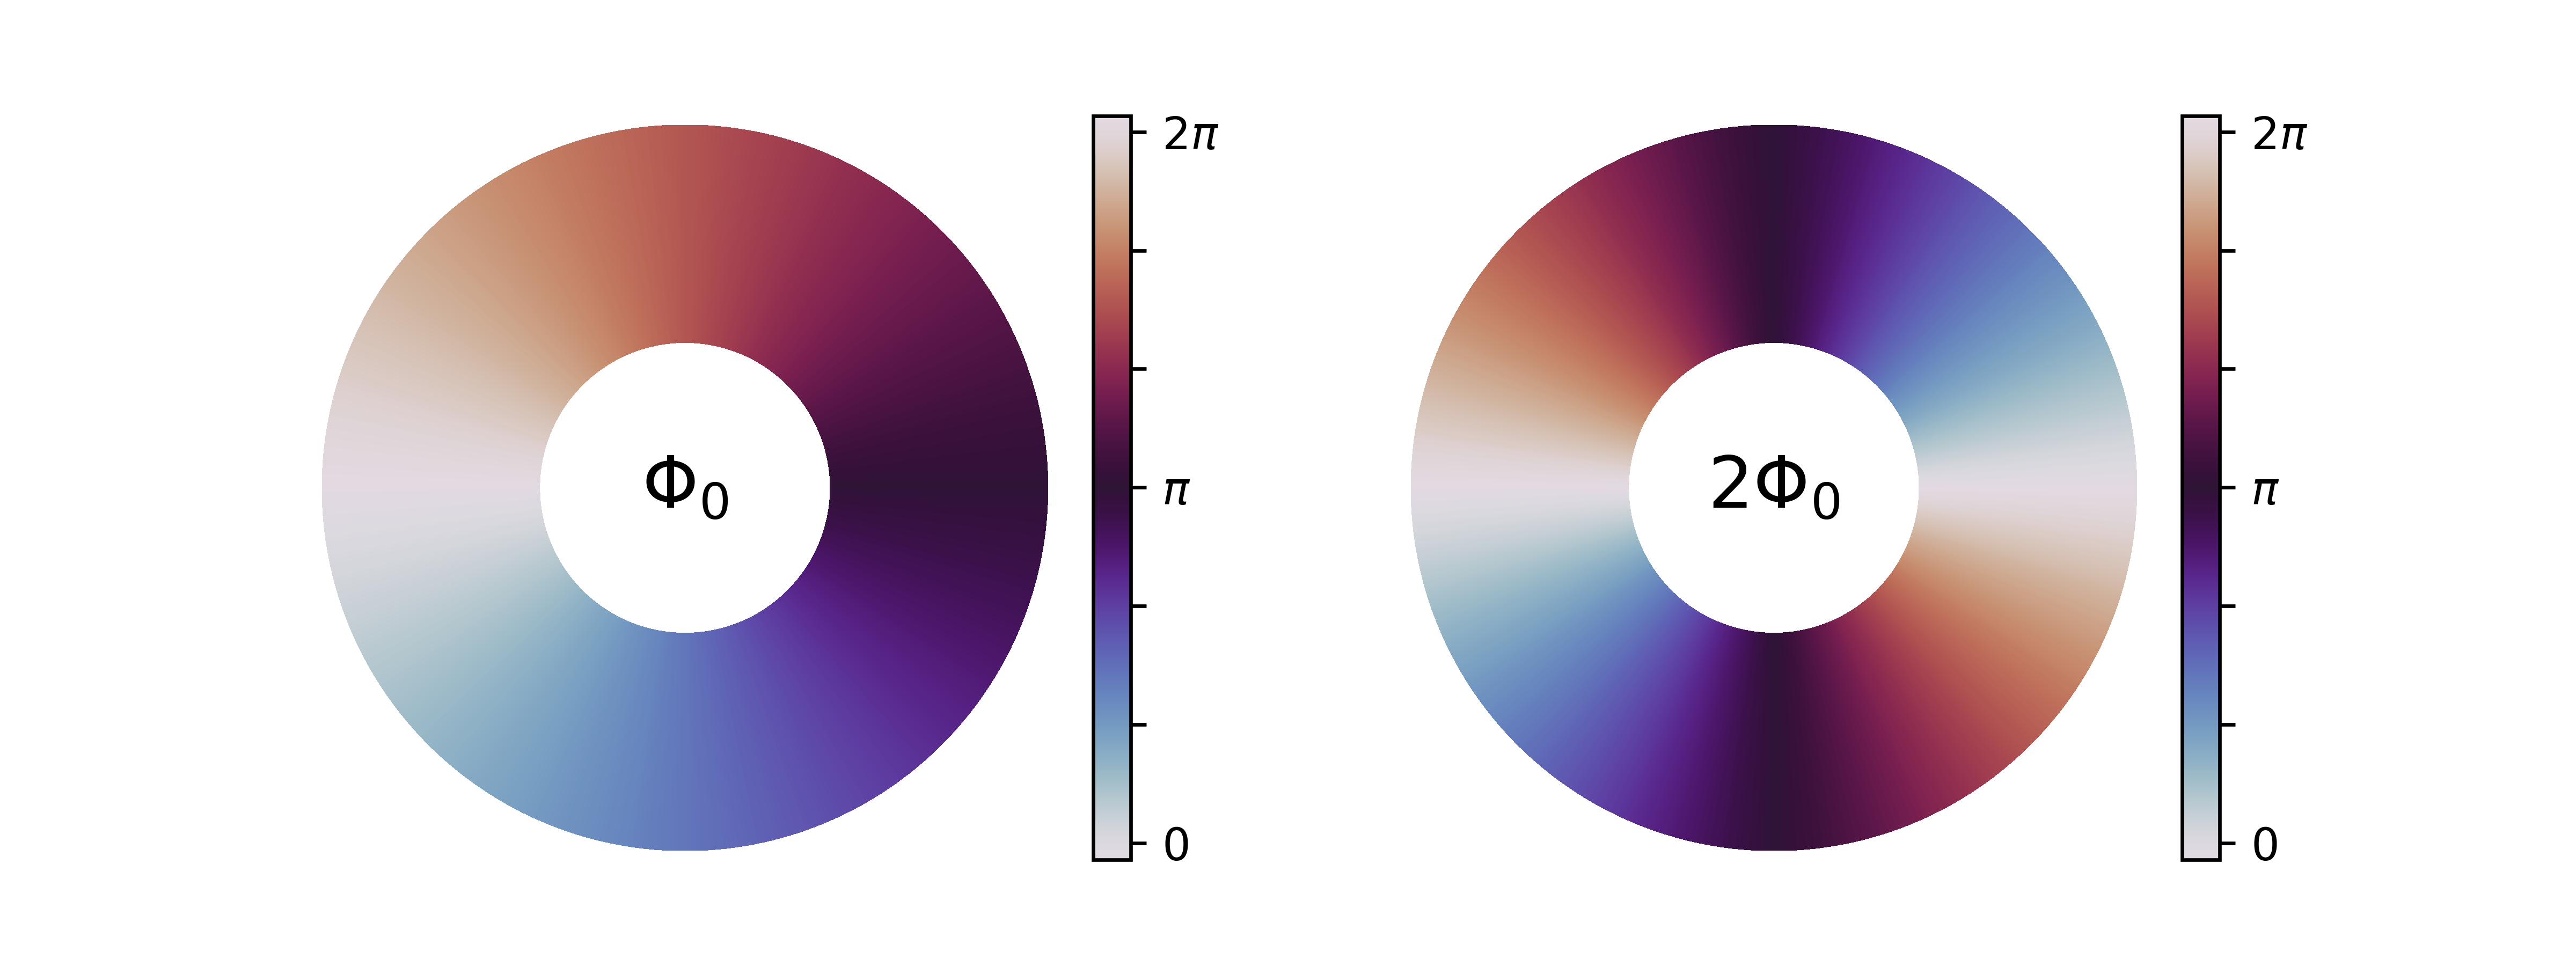
\includegraphics [width=1\textwidth] {coils}
	\caption{Распределение фазы волновой функции в сверхпроводящем кольце для различных значений магнитного потока.  }
	\label{img:coils}
\end{figure}
Квантование потока наглядно показывает, что во многих физических ситуациях, важных при описании сверхпроводниковых цепей, фаза оказывается очень тесно связанной с магнитным потоком. Экспериментально, квантование потока впервые наблюдалось в работе \cite{FluxQuant}  Связь между $\varphi$ и $\Phi$ носит примерно такой же характер, как связь между $n$ и полным зарядом $Q$ сверхпроводящего острова. Действительно, у сверхпроводящего острова к дискретному заряду $Q_n \!=\! n\cdot2e$ добавляется заряд $q\! = \!CV$, наведённый некоторым напряжением $V$ через какую-либо дополнительную ёмкость $C$, и полный заряд равен $Q\!=\!Q_n\!+\!q$. Похожим образом, <<внутренний>> поток $LI_m$, возникающий за счет индуктивного ответа в кольце на внешнее магнитное поле, складывается с внешним потоком $\Phi_{ext}$, и в результате получается дискретный <<полный>> поток $\Phi\!=\!n\Phi_0$. Но как создать какую-либо наведенную непрерывным образом фазу? Оказывается, что при использовании эффекта Джозефсона это становится возможным.
\subsection{Эффект Джозефсона: общие принципы}
Чтобы понять суть эффекта Джозефсона, рассмотрим два объемных сверхпроводника (берега), разделенных слоем диэлектрика. Будем называть такую систему джозефсоновским переходом (или SIS-переходом). Если этот слой достаточно толстый, то берега никак не связаны между собой. Начнем мысленно уменьшать толщину диэлектрического слоя, и рано или поздно возникнет туннельный эффект. Туннелировать могут как отдельные электроны (квазичастицы), так и куперовские пары, существующие независимо для каждого берега. Но куперовские пары имеют удвоенную массу по сравнению с квазичастичными возбуждениями. Поскольку вероятность прохожения барьера экспоненциально падает с ростом массы частицы, то при какой-то толщине $h_1$ барьер станет прозрачным только для квазичастиц, не пропуская куперовские пары. Квазичастицы не формируют конденсат, поэтому такое одноэлектронное туннелирование принципиально не будет отличаться от сходных процессов в нормальных металлах или полупроводниковых структурах. Туннельный ток будет зависеть от плотности состояний, и поэтому будет отличен от нуля только при $V\!>\!2\Delta$, что впервые наблюдалось в работе \cite{GiaeverGap}. Хоть процесс туннелирования куперовских пар весьма маловероятен, но тем не менее, барьер уже достаточно прозрачен, и можно сказать, что волновая функция отдельных электронов из одного берега частично проникает в другой. Продолжим уменьшать толщину диэлектрика. Оказывается, что при некоторой толщине $h_2\!<\!h_1$ возникает когерентность во всей электронной системе. Можно сказать, что куперовские пары образуются из электронов, принадлежащих двум разным металлам одновременно. Эти пары увлекаются в один или другой металл, а направление и  скорость их увлечения зависит от разности сверхпроводящих фаз между берегами. То есть, ненулевой сверхпроводящий ток возникает при $V\!=\!0$. Описанные процессы туннелирования схематично изображены на Рис.\:\ref{img:jj_tunn}. Из качественного рассмотрения может показаться, что одночастичный ток и ток конденсата должны возникать при одинаковой толщине барьера, но в действительности джозефсоновский ток наблюдается при меньшем нормальном сопротивлении, чем одночастичный. Это связано с влиянием тепловых флуктуаций, которые растут с увеличением $R$. Детальное описание можно найти в \cite{Barone}. Покажем, как этот ток зависит от разности фаз.
\begin{figure}
{\centering 
\hfill
\fontsize{22pt}{22pt}\selectfont
\def\svgwidth{3.5in}%
\input{images/JJ_disser.pdf_tex}
\hfill
}
\caption{SIS переход и различные процессы туннелирования через барьер.}
\label{img:jj_tunn}
\end{figure}
\subsection{Токо-фазовое соотношение}

%Прежде чем перейти к описанию эффекта Джозефсона, рассмотрим упрощенную модель электронной системы в сверхпроводнике в представлении зонной структуры. Прежде всего, имеется конденсат куперовских пар, то есть все пары находятся на одном энергетическом уровне, который можно выбрать за нулевой: $E=0$. Если разорвать пару, то возникает 2 квазичастичных возбуждения (электрона) c энергией $E>\Delta$, и если электрон видит частично прозрачный барьер, то он может протунеллировать из сверхпроводника. Также возможен процесс, когда уже имеющийся электрон с другой стороны барьера Вопрос о плотности состояний квазичастиц в зависимости от энергии может быть рассмотрен в теории БКШ, которая дает ответ:


Будем считать, что каждый из берегов имеет собственные состояния конденсата куперовских пар в нем, которые можно описать при помощи макроскопической волновой функции: $\Psi_R\! =\! \sqrt{\rho_R}e^{i\varphi_R}$ и $\Psi_L \!=\! \sqrt{\rho_L}
e^{i\varphi_L}$, где $\rho_R, \rho_L$ --- плотности частиц. Состояние всего конденсата можно искать в виде $\Psi = \Psi_L\ket{L}\!+\!\Psi_R\ket{R}$, что означает, что общий конденсат куперовских пар когерентно распределится так, чтоб минимизировать энергию всей системы. В базисе состояний $\ket{R}, \ket{L}$ гамильтониан системы можно записать в виде:
\begin{equation}
H = E_L\cdot \ket{L}\bra{L} + E_R\cdot \ket{R}\bra{R} + T\cdot\big[ \ket{L} \bra{R}+\ket{R}\bra{L}\big],
\end{equation}
где последний член описывает туннелирование системы как целого и означает, что потенциальный барьер достаточно прозрачен, и некоторые пары из конденсата могут состоять из электронов находящихся по разные стороны от барьера. Теперь можно решить уравнение Шредингера $i\hbar d\Psi/dt\! =\! H\Psi$, распадающееся на два уравнения для амплитуд $\Psi_L$~и~$\Psi_R$: 
\begin{align}
	i\hbar \frac{d\Psi_R}{dt} & =E_R\Psi_R+T\Psi_L, \nonumber \\
    i\hbar \frac{d\Psi_L}{dt} & =E_L\Psi_L+T\Psi_R.
    \label{eq: je_deriv}
\end{align} 
Подставим выражения для $\Psi_L$~и~$\Psi_R$, и получим ответ для плотности сверхпроводящего (джозефсоновского) тока через барьер $J_s={d\rho_R}/{dt}=-{d\rho_L}/{dt}$:
\vspace{-1pt}
\begin{equation}
J=\frac{2T}{\hbar}\sqrt{\rho_R \rho_L}\sin \varphi = J_c \sin \varphi,
\label{eq: cur-phase}
\end{equation}
где $\varphi = \varphi_L-\varphi_R$. Если считать $\rho_L$ и $\rho_R$ константами, что будет справедливо, например, в случае подключения к внешнему источнику тока, то величина $J_c$, называемая плотностью критического тока, зависит только от свойств перехода, а именно от типа сверхпроводника и ширины туннельного барьера. Микроскопическая теория дает следующее выражение для критического тока $I_c$ джозефсоновского перехода в случае нулевой температуры и одинаковых сверхпроводников с $\Delta_L=\Delta_R=\Delta$:
\begin{equation}
I_c = \frac{\pi \Delta}{2eR_n},
\end{equation}
где $R_n$ --- остаточное сопротивление на переходе при $T \ge T_c$. Впервые стационарный эффект Джозефсона наблюдался в работе \cite{StatJosephsonExp}.
Зависимость $J=J(\varphi)$ вида \eqref{eq: cur-phase} характерна не только для туннельного SIS-перехода, но и для многих других типов слабой связи (например, мост Дайема, SNS- и SSeS-переходы \cite{LikharevWL, CPhiR_review}). 
\subsection{Фазо-потоковое соотношение}
Выше было рассмотрено квантование магнитного потока в сплошном кольце. Рассмотрим, как меняется ситуация при прерывании кольца некоторым количеством SIS-переходов ($n$ штук), плоскости которых перпендикуляры плоскости кольца, см. Рис.\:\ref{img:ph-fl}. Будем считать, что внешнее магнитное поле невелико, и можно не учитывать его проникновение в область диэлектрика (которое приводит к необычным эффектам в переходах, см., например, \cite{Schmidt}, \S\:24). Выберем замкнутый контур $C$, пролегающий в глубине кольца, и запишем уравнение \eqref{eq:2GL} с учетом обращающегося в ноль мейсснеровского тока:
\begin{equation}
\label{eq: FFR}
\oint\displaylimits_{C}^{} \mathbf{A} d\boldsymbol{\ell} = \frac{\Phi_0}{2\pi}\oint\displaylimits_{C}^{}\nabla\varphi d\boldsymbol{\ell}
\end{equation}
Правая часть этого выражения содержит интеграл от градиента фазы вдоль контура. Однако, фаза не является непрерывной функцией, а скачкообразно меняется на переходах. Поэтому в таком виде вычислять интеграл нельзя. Разобъем контур $C$ на несколько отрезков кривой $A_iB_i, i=1,\ldots n$, таким образом исключая короткие отрезки контура $C$, лежащие внутри переходов, из контура интегрирования. Будем считать что левый интеграл при этом не изменяется:
\begin{equation}\label{eq:int_cAdl}
\oint\displaylimits_{C}^{} \mathbf{A} d\boldsymbol{\ell} = \sum_{i=1}^{n}\int\displaylimits_{A_i}^{B_i} \mathbf{A} d\boldsymbol{\ell},
\end{equation}
поскольку ширины переходов достаточно малы, а векторный потенциал не имеет никаких особенностей в коротких отрезках контура $C$, лежащих внутри переходов, так как токи и магнитные поля нулевые. Теперь вычислим правый интеграл как:
\begin{equation}
\label{eq:int_phi}
\begin{alignedat}{2}
\oint\displaylimits_{C}^{}\nabla\varphi d\boldsymbol{\ell} = \sum_{i=1}^{n}\int\displaylimits_{A_i}^{B_i}\nabla\varphi d\boldsymbol{\ell} = \sum_{i=1}^{n}\varphi_{B_i}-\varphi_{A_i} & = \\ =\varphi_{A_1} + \sum_{i=1}^{n-1}(\varphi_{A_{i+1}}-\varphi_{B_i}) - \varphi_{B_n} & = 2\pi k + \sum_{i=1}^{n}(\varphi_{A_{i+1}}-\varphi_{B_i}) = \\ 
& =2\pi k + \sum_{i=1}^{n}\delta\varphi_i,
\end{alignedat}
\end{equation}
В предпоследнем равенстве использовано условие однозначности волновой функции в виде $\varphi_{A_1} = \varphi_{A_{n+1}}-2\pi k$. Разности фаз на переходах обозначены как $\delta\varphi_i$. Подставляя \eqref{eq:int_cAdl} и \eqref{eq:int_phi} в \eqref{eq: FFR}, получаем искомое фазо-потоковое соотношение:
\begin{equation}
\label{eq: FFR_final}
\frac{2\pi\Phi}{\Phi_0} = 2\pi k + \sum_{i=1}^{n}\delta\varphi_i.
\end{equation}
Таким образом, поток в таком кольце не квантуется, но однозначно определяется разностями фаз на джозефсоновских переходах. Предположим, например, что джозефсоновские энергии переходов, входящих в кольцо, одинаковы и равны $E_J$, соответственно, равны и критические токи $I_c$. Тогда
\begin{equation}\label{eq: FFR_case}
\frac{2\pi}{\Phi_0}(\Phi_{ext}-LI_c\sin \delta\varphi)= 2\pi k + n\delta\varphi,
\end{equation}
и при заданных $L\text{ и }\Phi_{ext}$ можно найти такие $k \text{ и } \delta\varphi$, которые характеризуют разрешенные состояния системы. Если переходы различны, то разности фаз $\delta\varphi_i$ будут такими, чтобы токи через переходы $I_i=I_{ic}\sin\delta\varphi_i$ были одинаковыми. 
\begin{figure}
	\centering
		\fontsize{22pt}{22pt}\selectfont
		\def\svgwidth{3.5in}%
		\input{images/phase-flux2.pdf_tex}
	\caption{К выводу фазо-потокового соотношения.}
	\label{img:ph-fl}
\end{figure}
%\begin{figure}[ht] 
%	\centering
%	\includegraphics [width=1\textwidth] {coils_jj.png}
%	\caption{Распределение фазы волновой функции в сверхпроводящем кольце для различных значений магнитного потока.}
%	\label{img:coils_JJ}
%\end{figure}
\subsection{Энергия джозефсоновского тока. RSCJ-модель.}
Из уравнений \eqref{eq: je_deriv} можно получить следующее соотношение:
\begin{equation}
\frac{d\varphi}{dt} = \frac{2eV}{\hbar}.
\label{eq: dphidt}
\end{equation}
Таким образом, при конечном напряжении на контакте фаза начинает меняться с течением времени. Это так называемый нестационарный эффект Джохефсона, имеющий множество интересных применений, например генерация высокочастотного тока и создание стандарта напряжения. Используя полученное соотношение, можно рассчитать потенциальную (свободную) энергию, сосредоточенную в переходе:
\begin{equation}
\label{eq:EJ}  
E(\varphi) = \int_{0}^{t}I_sVdt = \int_{0}^{\varphi} I_c\sin \varphi' \frac{\hbar}{2e} {d\varphi'} = E_J(1-\cos\varphi).
\end{equation}
В последнем равенстве учтено что при нулевой фазе ток через переход не течет, и $E(0)=0$. Величина $E_J = {\hbar I_c}/{2e}$ называется \textit{джозефсоновской энергией} перехода. При малых значениях $\varphi$ энергия квадратично зависит от фазы: $E_J\approx E_J \varphi^2/2$, что дает возможность ввести эквивалентную линейную индуктивность перехода $L_{lin} = \Phi_0^2/2\pi I_c$. В более общем случае, джозефсоновская индуктивность зависит от фазы и определяется как $L_J = \Phi_0/(2\pi I_c \cos \varphi)$.
\begin{figure}[ht]
	{\centering
		\hfill
%		\subbottom[List-of-Figures entry][Туннельные процессы в SIS-переходе.\label{img:jj_tunnel}]{%
%			\input{images/JJ_disser.pdf_tex}}
%		\hfill
		\subbottom[List-of-Figures entry][RCSJ-модель перехода.]{%
			\input{images/RSCJ.pdf_tex}}
		\label{img:RCSJ}
		\hfill
		\def\svgwidth{2.2in}
		\subbottom[Частица в потенциале $U(\varphi)$.]{%
			\input{images/washboard.pdf_tex}}
		\label{fig: washboard}
		\hfill
	}
	\caption{RCSJ-модель джозефсоновского туннельного перехода.}
	\label{img:knuth_2}
\end{figure}

До сих пор мы рассматривали лишь энергию сверхпроводящего тока. Однако, для описания нестационарных процессов в реальных туннельных контактах такая модель недостаточна. Необходимо учитывать два дополнительных фактора: квазичастичное туннелирование и значительная емкость между двумя сверхпроводниками, неизбежно возникающая из-за малой толщины диэлектричекой прослойки (несколько десятков межатомных расстояний). Эти аспекты учитываются в феноменологической RCSJ-модели перехода, в которой параллельно с джозефсоновским элементом, энергия которого зависит от фазы согласно \eqref{eq:EJ}, включается эквивалентный резистор $R$, описывающий нормальное сопротивление квазичастичному току, и конденсатор $C$, см.\:Рис.\:\ref{img:RCSJ}. Полный ток через переход в такой схеме можно записать как:
\begin{align}
I &= I_C + I_J + I_R = \frac{\hbar C}{2e} \frac{d^2\varphi}{dt^2}+I_c\sin \varphi+ \frac{\hbar}{2eR}\frac{d\varphi}{dt}, \text{ отсюда получаем:}  \nonumber \\
0 & = m\frac{d^2\varphi}{dt^2} + f \frac{d\varphi}{dt} + \frac{d}{d\varphi}\big(E_J\cos \varphi+E_J\frac{ I}{I_c}\varphi\big), 
\end{align}
где введены обозначения $m=(\hbar/2e)^2 C$ и $f=(\hbar/2e)^2R^{-1}$. Полученное уравнение описывает динамику фазы в переходе как классическое движение частицы массой $m$ в жидкой среде с коэффициентом вязкости $f$ во внешнем потенциале стиральной доски $U(\varphi)=-E_J(\cos \varphi+I\varphi/I_c)$, что схематично отражено на Рис.\:\ref{fig: washboard}. Отметим некоторые характерные особенности динамики системы:
\begin{itemize}
	\item При отсутствии тока потенциал синусоидален, и частица локализуется в потенциальной яме, форма которой близка к параболической, и в этом случае может совершать малые колебания с частотой $\omega_p = (\sqrt{L_{lin}C})^{-1}$, называемой \textit{плазменной частотой перехода}. 
	\item Если увеличивать ток, то наклон потенциала растёт, потенциальная яма становится все более мелкой и пропадает. Частица начинает двигаться и будет разгоняться вдоль стиральной доски, пока не достигнет режима, в котором среднее значение $\langle V \rangle  \propto \langle d\varphi/dt \rangle$ постоянно и отлично от нуля. Характер её замедления при уменьшении тока (наклона) определяется параметром Маккамбера $\beta_c = \omega_p R C$, который показывает обратное число плазменных колебаний, которые система может совершить за время затухания $RC$ (при отсутствии тока).
	\item Если $\beta_c\ll1$, то при уменьшении тока частица практически не замедляется до тех пор, пока наклон не упадет практически до нуля. 
	\item Если $\beta_c\gg1$, то частица замедляется довольно значительно, так как трение играет существенную роль в её движении и скорость движения вдоль стиральной доски определяется средним наклоном. Полная остановка, однако, также произойдет лишь при $I=0$.
\end{itemize}
Перечисленные особенности находят подтверждение при измерении ВАХ переходов, полученных при фиксированном внешнем токе $I$, см., например, \cite{Schmidt}. 

Подведем итог классическому описанию джозефсоновского перехода. В зависимости от выбранного режима работы, такой переход может вести себя как нелинейный осциллятор, нелинейная индуктивность, зависящая от времени, либо демонстрировать еще более сложное поведение. Это делает его весьма интересным элементом даже с точки зрения классической схемотехники. Еще более нетривиальные эффекты возникают в том случае, если рассматривать разность фаз на переходе как квантовую степень свободы, которые мы кратко опишем далее. 
\section{Квантование электрических цепей}
\label{ch: Quant}

Как было сказано выше, при квантовом описании какой-либо сверхпроводящей системы число пар $\hat{n}$ на сверхпроводящем острове и фаза $\hat{\varphi}$ на этом острове могут рассматриваться как сопряженные переменные: $[\hat{\varphi}, \hat{n}]=i$. Возбуждения коллективной квантовой степени свободы при определенных условия оказываются самыми низкоэнергетическими (ниже 10 ГГц), и потому есть возможность экспериментально работать только с ними. В сверхпроводниках минимальная энергия одноэлектронного возбуждения не может быть меньше $2\Delta$, например, для алюминия имеем $2\Delta=3.52 k_b T_c\approx h\cdot80$ ГГц. Можно показать \cite{girvin2011circuit}, что частоты объемных плазменных колебаний попадают в терагерцовый диапазон, и поэтому их также можно исключить из рассмотрения. Фактически, мы будем иметь дело с бездисперсионными коллективными плазменными возбуждениями, и именно эти моды в итоге будут квантоваться. 
\subsection{Кубит. Двухуровневое приближение. Приближение вращающейся волны.}
\label{sec: qubit}
Простейшая квантовая система, например, спин $1/2$ в продольном магнитном поле, обладает одной степенью свободы и двумя собственными квантовыми состояниями. Обозначим состояния системы как $\ket{0}\equiv\begin{pmatrix} 1 & 0 \end{pmatrix}^{T} \text{и} \ket{1}\equiv\begin{pmatrix} 0&1 \end{pmatrix}^T$, а соответствующие собственные значения энергии как -$E_q/2$ и $E_q/2$. Тогда гамильтониан кубита записывается тривиально: $\hat{H}\!=\!\frac{-E_q}{2}\sz$. 

Согласно постулату квантовой механики, все возможные состояния кубита записываются как~$\ket{\psi}=\cos\frac{\theta}{2}\ket{0}+ 
e^{i\varphi}\sin\frac{\theta}{2}\ket{1}, 0 \le \theta \le \pi, 0 \le \varphi \le 2\pi $. Любая реальная система взаимодействует со своим окружением, поэтому состояния кубита необходимо описывать матрицей плотности:
\begin{equation}
\rho_q = \ket{\psi}\bra{\psi} =
\begin{pmatrix} \cos^2\frac{\theta}{2} & \cos\frac{\theta}{2}e^{-i\varphi}\sin\frac{\theta}{2}\\
\cos\frac{\theta}{2}e^{i\varphi}\sin\frac{\theta}{2}& \sin^2\frac{\theta}{2}
\end{pmatrix} = 
\begin{pmatrix} 1-\rho_{11} & \rho_{01}\\ \rho_{01}^*& \rho_{11}
\end{pmatrix}
\end{equation}
Последнее выражение можно обобщить и на случай смешанных состояний кубита, которые описывают статистический ансамбль. Поскольку матрицы Паули вместе с единичной матрицей составляют базис в пространстве матриц $2\times2$, то такую матрицу плотности можно записать в общем виде:
\begin{equation}
\rho_q = \frac{1}{2}(I+\vec{s}\cdot\vec{\sigma}),
\label{eq: rho_to_bloch}
\end{equation}
где $I$ --- единичная матрица, $\vec{\sigma}=\begin{pmatrix} \sigma_x & \sigma_y & \sigma_z \end{pmatrix}^{T}$ и
 $\vec{s}=\begin{pmatrix} s_x & s_y & s_z \end{pmatrix}^{T}$ --- трёхмерный вектор, называемый вектором Блоха. Для чистых состояний $\vec{s}=\begin{pmatrix} \sin\theta\cos\varphi & \sin\theta\sin\varphi & \cos\theta \end{pmatrix}^{T}$ можно представить как вектор из начала координат единичной длины, и все возможные положения конца этого вектора формируют единичную сферу --- сферу Блоха, см. Рис. \ref{img:bloch}.
\begin{figure}
 	\centering
 	\def\svgwidth{4in}
 	\input{images/Bloch_empty_3.pdf_tex}
 	\caption{Сфера Блоха. Точки на сфере соответствуют чистым состояниям кубита, точки внутри сферы --- смешанным состояниям.}
 	\label{img:bloch}
\end{figure} 

Квантовая двухуровневая система является простейшим объектом. В реальных экспериментах с СКЦ мы, как правило, работаем с многоуровневой системой. Но в некоторых физических ситуациях можно выделить два нижних уровня системы, и рассматривать систему внутри подпространства из основного и первого возбужденного квантовых состояний. 
Для этого необходимо делать двухуровневое приближение. 

Рассмотрим систему с собственными состояниями $\hat{H}_0\ket{n} = E_n\ket{n}$, под действием возмущения $\hat{V}(t)$. Учитывая поправку к собственным энергиям ${\tilde{E}_n}=E_n+\braket{n|\hat{V}|n}$, можно записать полный гамильтониан в виде:
\begin{equation}
\hat{H} = \sum_n\tilde{E}_n\ket{n}\bra{n} + \sum_{m \ne n}\textbf{}\ket{m}\bra{n}\braket{m|\hat{V}|n}. 
\end{equation} 
Оператор эволюции можно записать через повышающие и понижающие матрицы: $\hat{V} =   \sum_{m>n}\braket{m|\hat{V}|n}\hat{\sigma}_{mn}+\braket{n|\hat{V}|m}\hat{\sigma}_{nm}$. Тогда оператор эволюции возмущенной системы $U_0(t) = \exp(-\frac{i}{\hbar}(\tilde{E}_n\ket{n}\bra{n}))$ задаёт представление взаимодействия, гамильтониан в котором имеет вид:
\begin{equation}\label{eq: H_I}
\hat{H}_I = \sum_{m>n} e^{-{i}(\tilde{\omega}_n-\tilde{\omega}_m)t}\braket{m|\hat{V}|n}\hat{\sigma}_{mn} + \text{ c.c} 
\end{equation}
Если возмущение будет состоять из нескольких слагаемых, то соответствующие $\hat{H}_I$ могут не коммутировать, что сильно усложнит поиск аналитического решения для динамики системы и приведет к непоправимым последствиям. Однако, предположим, что $\hat{V}(t)\!=\!\hat{V}_0e^{i\omega t}$, где $\omega\!\approx\!\tilde{\omega}_{01}$. Тогда ясно, что наибольший вклад в оператор эволюции системы в представлении взаимодействия $\mathcal{T} \exp (-\frac{i}{\hbar}\int_0^t \hat{H}_I(t')dt')$ даёт слагаемое из \eqref{eq: H_I} с наиболее медленной зависимостью от времени. Все остальные члены дают интегралы от быстро осциллирующих функций, которые очень малы и не меняют характер динамики, заданной главным членом. Таким образом, мы можем сделать два приближения:
\begin{itemize}
	\item \textit{двухуровневое приближение} позволяет оставить в $H_I$ только члены $\braket{0|\hat{V}_0|1}\hat{\sigma}_{01} + e^{-2\omega t}\braket{1|\hat{V}_0|0}\hat{\sigma}_{10}$, пренебрегая переходами между остальными парами уровней, не попадающими в резонанс с возмущающим воздействием;
	\item \textit{приближение вращающейся волны} позволяет оставить только медленно меняющийся член $\braket{0|\hat{V}_0|1}\hat{\sigma}_{01}$.
\end{itemize}

Для того чтоб описывать СКЦ как кубит, необходимо, во-первых, уметь рассчитать её спектр в зависимости от параметров цепи и, во-вторых, уметь вычислить матричные элементы переходов под воздействием возмущений, например, внешнего электромагнитного поля. Теперь опишем общий формализм квантования цепи, а затем на некоторых примерах покажем, как осуществляются расчеты такого типа.
\subsection{Формальная процедура квантования цепи}	
Опишем общий подход к квантованию СКЦ \cite{vool2017introduction}. Будем рассматривать некоторую систему, состоящую из набора сверхпроводящих островов. Острова могут быть связаны взаимными емкостями и индуктивностями. Кроме того, некоторые из них могут образовывать джозефсоновскую связь. Поэтому, достаточно общим является представление такой системы в качестве электрической цепи, в которой имеются три типа элементов: емкости, индуктивности и джозефсоновские элементы (нелинейные индуктивности)\footnote[1]{Совсем недавно \cite{astafiev2012coherent} показана возможность создания т.н. центра когерентного квантового проскальзывания фазы, который является емкостным аналогом джозефсоновского перехода. Однако, создание квантовых цепей из таких элементов еще не вполне отработано. Их описание выходит за рамки данной работы.}. Как и в электротехнической цепи, в такой системе нужно подходящим образом выбрать некоторые независимые степени свободы, с помощью которых можно описать как классическую, так и квантовую динамику системы. Последовательность действий квантования системы состоит из следующих шагов:
\begin{enumerate}
\item Изобразим эквивалентную электрическую схему цепи. Схема будет состоять из N узлов (точек), связанных произвольным количеством элементов-двуполюсников, которые мы будем называть ребрами. Мысленно выделим емкостную и индуктивную части в общей схеме цепи. Поскольку любой реальный элемент имеет конечные размеры, и следовательно, паразитную емкость, то можно считать, что между каждой парой узлов включена емкость, и притом единственная. Среди всех узлов можно выделить \textit{активные} узлы, к которым подсоединены как емкостные, так и индуктивные элементы, и \textit{пассивные} узлы, к которым подсоединены только емкости.

\item Для каждого ребра введем величину $\Phi(t)=\int_{-\infty}^{t} v(t')dt'$, которую можно назвать магнитным потоком через ребро. Считается, что напряжение $v(-\infty)=0$ и плавно включается со временем. Тогда емкостную энергию можно записать как $C\dot{\Phi}^2/2$, что соответствует кинетической энергии частицы с кординатой $\Phi$. Для индуктивности эта величина в точности совпадает с запасённым в ней магнитным потоком, и индуктивная энергия $(\Phi-\widetilde{\Phi})^2/2L$ играет роль потенциальной энергии, где $\widetilde{\Phi}$ --- некоторый внешний поток. 
\item Выберем один из активных узлов емкостной подсистемы в качестве заземленного узла, и выберем только те емкости, которые единственным образом соединяют земляной узел со всеми остальными узлами подсистемы. Эти емкости составят \textit{остовное дерево} $T$. Тогда для любого другого узла $n$ можно ввести т.н. \textit{узловой поток} $\phi_n$, который равен сумме потоков всех емкостей, через которые нужно пройти от земляного узла до узла $n$. Связь между потоком через некоторое ребро $\Phi_b$ и потоками через узлы этого ребра $\phi_n, \phi_{n'}$ даётся соотношением:
\begin{equation}\label{eq: Phiphi}
\begin{aligned}
	\Phi_{b\in T} &= \phi_n-\phi_{n'}, \\
	\Phi_{b\notin T} &= \phi_n-\phi_{n'} + \widetilde{\Phi}_b,
\end{aligned}
\end{equation}
где внешний поток ${\Phi}_b$ учитывается в том случае, когда добавление ветви $b$ образует индуктивную петлю.
\item Используя соотношения \eqref{eq: Phiphi}, запишем полную энергию индуктивной и емкостной подсистемы через переменные $\vec{\phi}=(\phi_1\ldots\phi_N)^T$.  Энергия индуктивной подсистемы примет вид:
\begin{equation}
E_L(\vec{\phi}) = \frac{1}{2}{\vec{\phi}^{\mathsmaller T}} \mathbf{L^{-1}}\vec{\phi} + \sum_b \frac{\phi_n-\phi_{n'}}{L_b}\widetilde{\Phi}_b.
\end{equation}
Первое слагаемое представляет собой вклад в энергию непосредственно от индуктивностей. Матрица индуктивности $\mathbf{L}$ размера $(N-1)\!\times\!(N-1)$ симметричная и сконструирована следующим образом: недиагональные элементы $(i,j)$ равны $-\sum L_{ij}$, где $L_{ij}$ - все индуктивности, соединяющие узлы $i$ и $j$; диагональные же элементы равны сумме всех недиагональных элементов на соответствующей строке (или в столбце), взятой с противоположным знаком. Второе слагаемое --- это энергия каждой индуктивности, которая находится в ветви с внешним потоком $\widetilde{\Phi}_b$. Энергия емкостной подсистемы примет вид:
\begin{equation}
E_C(\dot{\vec{\phi}})= \frac{1}{2} {\dot{\vec{\phi}}^{\mathsmaller T}} \mathbf{C^{-1}} \dot{\vec{\phi}}
\end{equation}
где матрица емкости $\mathbf{C}$ строится аналогично матрице индуктивности.
\item Полученные выражения позволяют записать лагранжиан системы $\mathcal{L} = E_C-E_L$ и найти классические уравнения движения $\frac{d}{dt}\frac{\partial\mathcal{L}}{\partial\dot{\phi_n}}=\frac{\partial\mathcal{L}}{\partial{\phi_n}}$. Поскольку нас интересует квантовое описание системы, необходимо найти обобщенные импульсы $q_n = \partial\mathcal{L}/\partial{\dot\phi_n}$,  и записать гамильтониан $H = q_n\phi_n-\mathcal{L}$. Сколько независимых степеней свободы будет иметь система? Чтобы ответить на этот вопрос, необходимо заметить, что для любого пассивного узла $\partial \mathcal{L}/\partial{\phi_n}=0$, а поэтому $q_n$ является константой, и фактически, даннная степень свободы вырождена. Таким образом, если число активных узлов $P$, то полное число степеней свободы $P-1$.
\item Заменяя координаты (узловые потоки) и импульсы (узловые заряды) на сопряженные операторы $\phi\rightarrow\hat{\phi}$~и~$q\rightarrow\hat{q} = -i\hbar\frac{\partial}{\partial \phi}$, получаем гамильтониан квантовой цепи. Далее можно найти стационарные состояния, их энергии, матричные элементы переходов, и описать динамику системы.
\end{enumerate}
Далее мы рассмотрим некоторые базовые типы СКЦ. Как правило, они достаточно просты, и можно записать гамильтониан практически сразу, без предварительных шагов. Однако, следование общему формализму квантования необходимо для правильного описания более сложных цепей со многими степенями свободы. 
   
Базовые типы СКЦ, далее просто кубитов - это зарядовый кубит, фазовый кубит, потоковый кубит, трансмон и вч-СКВИД. Кратко опишем свойства каждого из этих кубитов.
\subsection{Зарядовый кубит}\label{charge_q}
	\begin{figure}[b]
		{ \raggedleft
			\hfill
			\def\svgwidth{2in}
			\fontsize{19pt}{19pt}\selectfont
			\subbottom[List-of-Figures entry][\label{img: CPB_scheme}]{%
				\input{images/CPB_qubit.pdf_tex}}
			\hfill
			\def\svgwidth{4in}
			\subbottom[\label{img: CPB_spectrum}]{%
				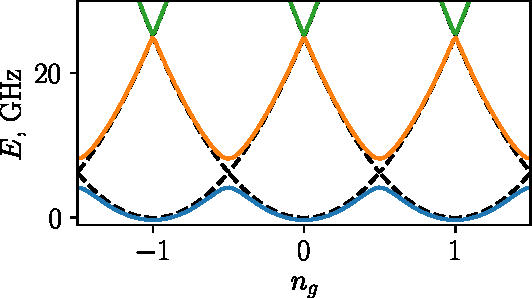
\includegraphics{images/CPB_spectrum.pdf}}
			
			\hfill
		}
		\caption[Схема зарядового кубита и его спектр.]{Зарядовый кубит: a) Эквивалентная схема кубита, б) Спектр кубита: три нижних энергетических уровня в зависимости от $n_g$. $E_C/h=\!=\!50 \text{ ГГц}, E_J/h\!=\!4\text{ ГГц}$. Пунктирная линия показывает классическую зарядовую энергию в отсутствие туннелирования.}
		\label{img: CPB}
		
	\end{figure}
Зарядовый кубит, или <<ящик>> для куперовских пар - это система, представляющая из себя джозефсоновский переход с энергией $E_J$, последовательно соединённый с емкостью. Эквивалентная схема такого кубита изображена на Рис.\ref{img: CPB}\subcaptionref*{img: CPB_scheme}. Образуется изолированный остров (выделен синим цветом), и если его емкость достаточно мала, то изменение числа куперовских пар на единицу сильно меняет энергию системы.  Введем зарядовую энергию конденсатора $E_C = 4e^2/C$; она включает в себя всю эффективную емкость острова, в т.ч. джозефсоновскую емкость. Также к острову подключен внешний источник, который может создавать наведенный заряд $n_g = C_gV_g/2e$.   Остовное дерево и земля выбираются тривиально, и понятно, что единственная степень свободы задается операторами фазы $\hat{\varphi}_1\!=\!2\pi/\Phi_0\!\cdot\!\hat{\phi}_1$ и заряда $\hat{n}_1\!=\!\hat{q}_1/2e$, далее индекс будет опущен за ненадобностью.~Гамильтониан системы имеет вид:
\begin{equation}
\hat{H}_{CPB} = \frac{E_C}{2}(\hat{n}-n_g)^2-E_J \cos \hat{\varphi}.
\end{equation}
Для нахождения спектра можно выбрать как фазовый базис, в котором $\hat{\varphi}\!=\!\varphi$, так и базис чисел куперовских пар (зарядовый базис), в котором $\hat{n}\!=\!n$. Начнем рассмотрение с зарядового базиса и выясним, как записать оператор $\cos\hat{\varphi}$. Заметим, что:
\begin{equation}
e^{i\hat{\varphi}}\ket{n} = e^{i\hat{\varphi}}\sum_n e^{in\hat{\varphi}}\ket{\varphi} = \ket{n+1},
\end{equation}
поэтому имеем:
\begin{equation}\label{eq: cosphi}
\cos \hat{\varphi} = \frac{1}{2}(e^{i\hat{\varphi}}+e^{-i\hat{\varphi}}) =
\frac{1}{2}\sum_n\Big(\ket{n+1}\bra{n} + \ket{n}\bra{n+1}\Big),
\end{equation}
где во втором слагаемом последнего выражения был сдвинут индекс суммирования $n \rightarrow n+1$. Гамильтониан можно записать в виде:
\begin{equation}
\hat{H}_{CPB} = \frac{E_C}{2}\sum_n(n-n_g)^2\ket{n}\bra{n}-\frac{E_J}{2} \sum_n\Big(\ket{n+1}\bra{n} + \ket{n}\bra{n+1}\Big).
\end{equation}
Получив его в такой форме --- диагональная часть плюс туннельный гамильтониан --- можно сразу сказать, как будет выглядеть собственные уровни энергии: в случае полуцелых $n_g$ два состояния с соседними $n$, вырождены. Новые собственные состояния сдвинуты на $\pm E_J/2$. Численно рассчитанный спектр изображен на Рис. \ref{img: CPB}\subcaptionref*{img: CPB_spectrum}. Сделаем двухуровневое приближение, то есть будем рассматривать подсистему из двух зарядовых состояний $\ket{0}$ и $\ket{1}$, и считать, что $n_g \approx 0.5$. Тогда гамильтониан примет вид: 
\begin{equation}
H_q = \frac{E_C}{2}(n_g-1/2)\sz-\frac{E_J}{2}\sx, 
\end{equation}
а новые собственные состояния системы можно записать через параметр $\theta = \arctan(\frac{2E_J}{E_C(n_g-1/2)})$ следующим образом: 
\begin{equation}
\begin{aligned}
\ket{g} & = \sin \frac{\theta}{2} \ket{0} + \cos \frac{\theta}{2} \ket{1}, \\
\ket{e} & = \cos \frac{\theta}{2} \ket{0} - \sin \frac{\theta}{2} \ket{1}
\label{eq: charge_e}
\end{aligned}
\end{equation}
Как и следовало ожидать, состояния максимально гибридизованы в окрестности $n_g\!=\!1/2$. 

Считается, что в пределе зарядового кубита $E_J < E_C$, то есть туннеллирование проявляется лишь между соседними зарядовыми состояниями. Отчасти исследование именно такого режима связано с тем, что зарядовый кубит --- исторически первый кубит, который был продемонстрирован в эксперименте \cite{nakamura1999coherent}. Для считывания используются такие методы, как джозефсоновский цикл квазичастичной генерации через дополнительный пробный барьер, подключенный к острову, а также одноэлектронный транзистор \cite{pashkin2009josephson}. Для такого считывания требуется, чтоб энергии зарядовых состояний при фиксированном $n_g$ сильно отличались друг от друга, то есть, ярко выраженный эффект кулоновской блокады. С этим связан и существенный недостаток зарядового кубита --- слишком высокая чувствительность к зарядовому шуму, влияющему на $n_g$. Различные паразитные двухуровневые системы в кремниевой подложке обладают электрическим дипольным моментом, влияющим на энергию кубита. Кроме того, попадание любой случайной квазичастицы на остров сильно сдвигает рабочую точку и делает длительную когерентную манипуляцию невозможной. В дальнейшем мы рассмотрим модификацию зарядового кубита с малой зарядовой энергией --- кубит-трансмон, работающий в так называемом пределе плоских зон, когда чувствительность к зарядовым шумам практически исчезает.
\subsection{Фазовый кубит}
Еще один тип кубитов, активно использовавшийся в 2000-х гг. --- фазовые кубиты \cite{martinis2009superconducting}. Фазовый кубит представляет собой смещенный постоянным током джозефсоновский переход. Точный контроль значения тока смещения $I$ позволяет хорошо контролировать глубину ямы в потенциале стиральной доски, см.~Рис. \ref{fig: washboard} и таким образом, регулировать число квантовых состояний, локализованных в яме. Пара нижних уровней и используется в качестве кубитной подсистемы. Управление осуществляется внешним высокочастотным током, подаваемым на переход. Считывание состояний \cite{steffen2006measurement} осуществляется при помощи дополнительной потоковой линии контроля: короткий импульс постоянного тока дополнительно наклоняет потенциал стиральной доски. Величина этого наклона подобрана таким образом, чтобы переход в состоянии $\ket{1}$ имел очень высокую вероятность протуннелировать через потенциальный барьер, который на время импульса становится значительно более прозрачным. В то же время, вероятность туннелирования состояния $\ket{0}$ должна быть исчезающе мала. Этого не так сложно добиться, учитывая тот факт, что согласно квантовой механике, в любой сколь угодно мелкой одномерной потенциальной яме имеется связанное состояние. Если туннелирование произошло, то джозефсоновский переход начинает движение вдоль стиральной доски, и на нём появляется ненулевое напряжение, и как следствие, высокочастотная компонента тока. Её можно обнаружить при помощи дополнительного считывающего пч-СКВИДa, что и делается в эксперименте. Как легко заметить, такое считывание разрушает кубит, и требуется конечное время для последующей инициализации в состоянии $\ket{0}$. Кроме того, шум тока смещения может вызывать значительное изменение потенциала, и как следствие, дефазировку кубита. Несмотря на имеющиеся недостатки, в работе с данными кубитами достигнут серьезный прогресс: были созданы 4-кубитные квантовые процессоры \cite{lucero2012computing}, реализующие простейшие квантовые алгоритмы, например, разложение на множители числа 15. В настоящий момент интерес к данному типу кубитов несколько уменьшился, однако, их исследование в достаточной мере способствовало развитию физики СКЦ.
 
\subsection{Потоковый кубит}
В зарядовом кубите, который мы рассмотрели ранее, реализуется суперпозиция состояний с разными числами куперовских пар на острове. Похожим образом можно создать суперпозицию состояний с различным значением магнитного потока в сверхпроводящей петле с включенными в неё джозефсоновскими переходами. Данная концепция была предложена в работе \cite{mooij1999josephson}, а кубит получил название <<кубит с незатухающим током>> и впоследствии упоминался упрощенно как \textit{потоковый кубит}. Схема потокового кубита с тремя джозефсоновскими переходами приведена на Рис.~\ref{img: flux_q}\subcaptionref*{img: fluxQ_scheme}. Обычно два перехода одинаковые, а площадь третьего перехода составляет $\alpha$ от площади больших переходов. Обычно выбирается $0\!<\!\alpha\!<\!1$. 
\begin{figure}[b]
	{ \raggedleft
		\hfill
		\def\svgwidth{3in}
		\fontsize{19pt}{19pt}\selectfont
		\subbottom[List-of-Figures entry][\label{img: fluxQ_scheme}]{%
			\input{images/3jj_qubit_ed.pdf_tex}}
		\hfill
		\subbottom[\label{img: flux_spectrum}]{%
			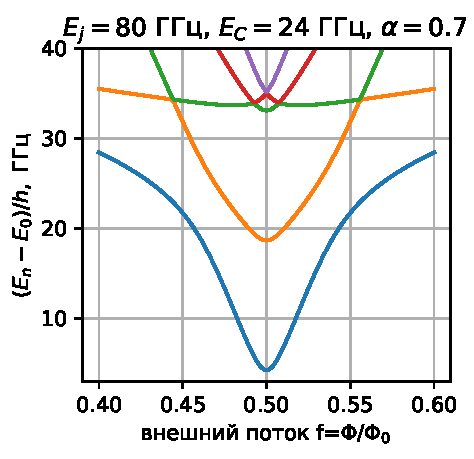
\includegraphics[width=0.5\textwidth]{images/3jj_spectrum_2.pdf}}
		
		\hfill
	}
	\caption[Схема потокового кубита и его потенциальная энергия.]{Потоковый кубит: a) Эквивалентная схема кубита, б) Спектр кубита: зависимости низших энергетических уровней в зависимости от $\Phi/\Phi_0$.}
	\label{img: flux_q}
	
\end{figure}

Запишем лагранжиан системы, используя операторы потока в узлах $\phi_i, i=\{1,2\}$ и их фазовые аналоги $\varphi_i=2\pi\phi_i/\Phi_0$:
\begin{multline}\label{eq: Lagr_flux}
{\mathcal{L}} = \frac{C}{2}
\begin{pmatrix}\dot{\phi}_1 &\dot{\phi}_2\\
	\end{pmatrix}
\begin{pmatrix}
	2 & -1\\ 
	-1 & \alpha+1 \\
\end{pmatrix}
\begin{pmatrix}\dot{\phi}_1\\\dot{\phi}_2\\\end{pmatrix}
%\Big[\frac{{\dot{\phi}}^2_1}{2}+ \frac{({ {\dot{\phi}}_2-{\dot{\phi}}_1})^2}{2} + \alpha\frac{{\dot{\phi}}_2^2}{2}\Big]
 + \\ + E_J\Big[ \cos(\varphi_1)+\cos(\varphi_2-\varphi_1+2\pi\frac{\Phi}{\Phi_0})+\alpha\cos(\varphi_2)\Big] 
\end{multline}
Введем обобщенные импульсы, которые в данном случае соответствуют числам куперовских пар на островах с потоками $\phi_1$ и $\phi_2$: 
\begin{equation}
\centering
\begin{aligned}
q_1 = 2en_1 & = \frac{\partial\mathcal{L}}{\partial\dot{\phi}_1} = {C}(2\dot{\phi}_1-\dot{\phi}_2) \\
q_2 = 2en_2 & = \frac{\partial\mathcal{L}}{\partial\dot{\phi}_2} = {C}((\alpha+1)\dot{\phi}_2-\dot{\phi}_1),
\end{aligned}
\end{equation}
которые для удобства дальнейших преобразований можно записать также в матричной форме: 
\begin{equation}
%\mathbf{n} = \frac{C}{2e}\mathbf{M\dot{\boldsymbol{\phi}}}, \
\mathbf{\dot{\boldsymbol{\phi}}} = \frac{2e}{C}\mathbf{M^{-1}}\mathbf{n},\ \text{где } \mathbf{M}=\begin{pmatrix}
2 & -1\\ 
-1 & \alpha+1 \\
\end{pmatrix}, \mathbf{n} = \begin{pmatrix}n_1\\n_2\\\end{pmatrix}, 
\mathbf{\dot{\boldsymbol{\phi}}} = \begin{pmatrix}\dot{\phi}_1\\\dot{\phi}_2\\\end{pmatrix}.
\end{equation}
Теперь можно записать гамильтониан системы $H(\mathbf{n}, \boldsymbol{\varphi}) = \mathbf{n^{\mathsmaller T}}\dot{\boldsymbol{\phi}}(\mathbf{n})-\mathcal{L}(\dot{\boldsymbol{\phi}}(\mathbf{n}), \boldsymbol{\varphi})$:
\begin{equation}\label{eq: Ham_flux}
H = \frac{E_C}{2}\mathbf{n^{\mathsmaller T}}\mathbf{M^{-1}}\mathbf{n}-E_J\Big[ \cos\varphi_1+\alpha\cos\varphi_2+\cos(\varphi_2-\varphi_1+2\pi\frac{\Phi}{\Phi_0})\Big]
\end{equation}
Первое слагаемое уравнения \eqref{eq: Ham_flux}, содержащее кинетическую энергию, выраженную через обезразмеренную матрицу емкости $\mathbf{M}$, применимо к любой системе, не содержащей экзотических элементов типа нелинейных емкостей, и может записываться практически сразу, минуя стадию построения лагранжиана. При этом операторы $n_i$ соответствуют числу куперовских пар на островах кубита. В данном случае мы считали также, что через замкнутую петлю кубита может быть приложен внешний магнитный поток $\Phi$. Из соотношения \eqref{eq: FFR_final} следует, что поток нужно включить в одно из слагаемых, описывающих джозефсоновскую энергию переходов. 

Получив выражение для гамильтониана системы, можно рассчитать энергетический спектр в зависимости от внешнего потока. Используя выражение \eqref{eq: cosphi}, можно записать гамильтониан в базисе зарядовых состояний:
\begin{equation}
\begin{aligned}
H = \frac{E_C}{2}&\sum_{n}\ket{n}_1\!\ket{n}_2\mathbf{M}^{-1}\bra{n}_2\!\bra{n}_1-\\\frac{E_J}{2}\Big[&\sum_{n}\ket{n+1}_1\!\ket{I}_2\!\bra{I}_2\bra{n}_1 +\ket{n}_1\!\ket{I}_2\!\bra{I}_2\!\bra{n+1}_1+\ldots\Big]
\end{aligned}
\end{equation}
где выражение типа $\ket{\cdot}_1\!\ket{\cdot}_2$ означает тензорное произведение векторов, соответствующих зарядовым состояниям островов 1 и 2. Кроме того, ряд слагаемых, входящих в джозефсоновскую энергию, опущен, поскольку они конструируются аналогично приведенному в формуле слагаемому с $\cos\varphi_1$. Такая запись гамильтониана позволяет перейти к численному решению проблемы. Выбирается некоторый базис зарядовых состояний от $-N$ до $N$ зарядов на острове, гамильтониан записывается как матрица размером $(2N+1)^2\times (2N+1)^2$, диагональные члены соотвествуют зарядовой энергии, а недиагонильные члены туннельного типа --- джозефсоновской энергии. После этого находятся собственные векторы и собственные значения гамильтониана, которые и дают спектр системы в зависимости от $\Phi$ в качестве параметра. Пример рассчитанного спектра приведен на Рис.\:\ref{img: flux_spectrum}. Можно заметить, что система обладает очень большим ангармонизмом: частота перехода 0-1 гораздо ниже частоты перехода 1-2. 

Также достаточно полезно рассчитать спектр и в фазовом базисе. Для этого зарядовые операторы необходимо записать в виде $n_1=-i\partial/\partial\varphi_1$. При этом уравнение на собственные энергии $H\ket{\Psi(\varphi_1, \varphi_2)}=E\ket{\Psi(\varphi_1, \varphi_2)}$ примет вид дифференциального уравнения в частных производных, которое можно решать численно при помощи некоторой разностной схемы. Один из вариантов такой схемы для сетки с шагом $h_1$ по фазе $\varphi_1$ и с шагом $h_2$ по фазе $\varphi_2$ имеет вид: 
\begin{equation}\label{eq: diff_scheme}
\newcommand{\pd}[2]{\frac{\partial#2}{\partial #1}}
\newcommand{\pdd}[2]{\frac{\partial^2#2}{\partial#1^2}}
\newcommand{\pmx}[3]{\frac{\partial^2#3}{\partial#1\partial#2}}
\newcommand{\vp}{\varphi}
\begin{aligned}
&\pdd{\vp_1}{\Psi(\varphi_1,\varphi_2)} = \frac{\Psi(\vp_1^{i-1}, \vp_2^i) -2\Psi(\vp_1^{i}, \vp_2^i) + \Psi(\vp_1^{i+1}, \vp_2^i)}{h_1^2}\\
&\pdd{\vp_2}{\Psi(\varphi_1,\varphi_2)} = \frac{\Psi(\vp_1^{i}, \vp_2^{i-1}) -2\Psi(\vp_1^i, \vp_2^i) + \Psi(\vp_1^{i}, \vp_2^{i+1})}{h_2^2}\\
&\pmx{\vp_1}{\vp_2}{\Psi(\varphi_1,\varphi_2)} = \pmx{\vp_2}{\vp_1}{\Psi(\varphi_1,\varphi_2)} = 
\pd{\vp_1}{}\frac{\Psi(\vp_1,\vp_2^{i+1}) - \Psi(\vp_1,\vp_2^{i-1})}{2h_2} = \\
&= \frac{\Psi(\vp_1^{i+1},\vp_2^{i+1}) - \Psi(\vp_1^{i+1},\vp_2^{i-1})}{4h_2h_1} - \frac{\Psi(\vp_1^{i-1},\vp_2^{i+1}) - \Psi(\vp_1^{i-1},\vp_2^{i-1})}{4h_2h_1} 
\end{aligned}
\end{equation}
Получившиеся собственные векторы покажут распределение собственных состояний кубита по различным фазам (т.е. состояниям с определенными фазами). Примеры такого распределения для основного состояния $\ket{g}$ и первого возбужденного состояния $\ket{e}$ приведены на Рис. \ref{img: 3jj_vs}. Видно, что эти состояния образуются за счет когерентного квантового туннелирования системы между двумя потенциальными ямами. 
\begin{figure}[h]\center
	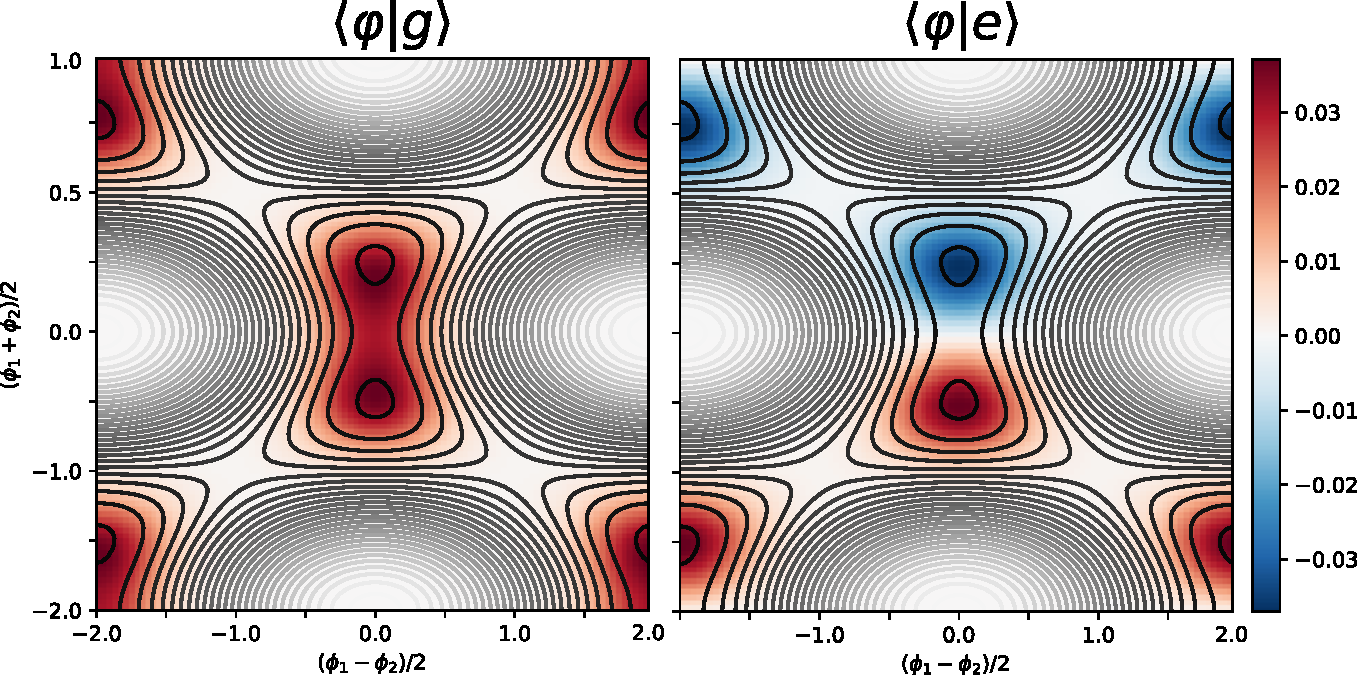
\includegraphics[width=0.95\textwidth]{images/3jj_vs.pdf}
	\caption{Волновая функция основного и первого возбужденного состояний потокового кубита при $\Phi=\Phi_0/2$. Линии уровня отображают потенциальную энергию.}
	\label{img: 3jj_vs}
\end{figure}
Высота барьера между двумя потенциальными ямами определяется параметром $\alpha$, и при $\alpha=0.5$ барьер исчезает. Поэтому данный параметр значительно влияет на собственные значения энергии и должен определяться достаточно точно, что может оказаться сложной задачей, особенно при использовании маленьких джозефсоновских переходов размерами порядка 200$\times$200 нм. Поэтому, как правило, воспроизводимость потоковых кубитов оказывается недостаточно хорошей. Также очевидно, что вне точки $\Phi=\Phi_0/2$ кубит восприимчив к потоковому шуму, что неизбежно будет вызывать дефазировку. Тем не менее, потоковый кубит остается достаточно интересен, прежде всего, за счет большого ангармонизма по сравнению с трансмоном, речь о котором пойдет ниже.  
\subsection{Трансмон} Рассмотренный в разделе \ref{charge_q} зарядовый кубит обладал многими несовершенствами. Попытки развития и соверщенствования даннго кубита привели к созданию кубита-трансмона. Трансмон --- это зарядовый кубит, шунтированный большой емкостью, у которого $E_C \ll E_J$~(обычно в 50 раз и более). Идея создания такого кубита впервые появилась в \cite{cottet2002implementation}, позднее было проведено подробное теоретическое исследование данных кубитов \cite{koch2007charge} и практически сразу же последовали первые эксперименты c трансмонами \cite{transmon}. Для того, чтобы проиллюстрировать необходимость такой модификации, приведем на Рис.~\ref{img: disp_vs_anh} относительный  aнгармонизм трансмона $(\omega_{10}-\omega_{21})/\omega_{10}$ и относительное изменение частот нижних переходов трансмона при изменении наведенного заряда $n_g$, то есть величину $|\omega_{i0}(n_g=e)-\omega_{i0}(n_g=0)|/\omega_{i0}(n_g=0)$ .  для различных значений отношения $E_C/E_J$. При уменьшении этого отношения уменьшается ангармонизм кубита.
\begin{figure}[h]\center
	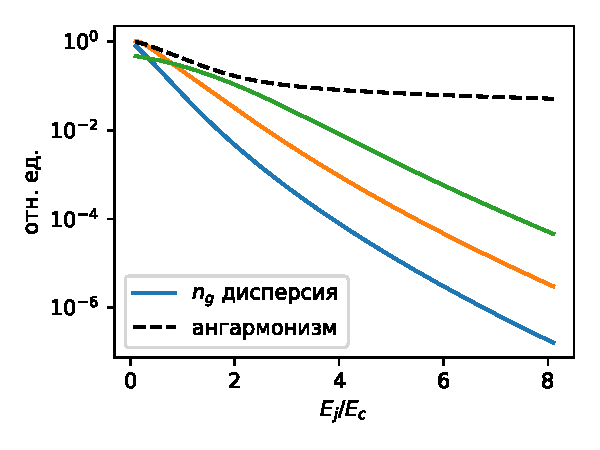
\includegraphics[width=0.75\textwidth]{images/disp_vs_anh.pdf}
	\caption{Изменение относительной зарядовой дисперсии для переходов 0-i трансмона и изменение ангармонизма основного перехода 0-1 в зависимости от отношения $E_J/E_C$. $E_C/h = 2$~ГГц}
	\label{img: disp_vs_anh}
\end{figure}
Для значений $E_C/E_J \approx 5$ кубит становится более похожим на гармонический осциллятор с относительно слабой нелинейностью в 5-10\% --- казалось бы, в таком эффекте нет никакой практической пользы. Но основным положительным эффектом от уменьшения $E_C/E_J$ является экспоненциально резкое падение зависимости энергетических уровней от $n_g$ --- так называемой зарядовой дисперсии. Особенно резко она уменьшается именно для низколежащих уровней, которые и используются на практике в качестве уровней кубита. Таким образом, удается достичь такого режима, когда ангармонизм еще достаточно большой и во многих ситуациях можно пренебречь верхними уровнями (или учесть их слабое влияние на динамику заселенности двух нижних уровней), и в то же время нежелательная зарядовая чувствительность практически подавлена. По этой причине для трансмонов характерны большие времена релаксации и декогеренции по сравнению как с зарядовыми, так и с потоковыми кубитами. Использование трансмонов при создании многокубитных схем оказалось весьма плодотворным, так как удалось разработать универсальные процессоры из 10 и более кубитов с полным контролем квантовых состояний. Однако, необходимо отметить, что во многих задачах трансмон нужно рассматривать как слабо нелинейный гармонический осциллятор, учитывая таким образом вклад верхних уровней. Например, при быстрых однокубитных операциях с трансмоном серьезную проблему представляют утечки заселенности кубита на второй возбуждённый уровень, которые необходимо предотвращать при помощи специальной коррекции управляющих импульсов. 

\subsection{вч-СКВИД}
Высокочастотный СКВИД - это прибор, представляющий собой джозефсоновский переход, шунтированный линейной индуктивностью $L$. Данный прибор изначально был предложен в 1965 г. для высокоточных измерений магнитного поля. Рассмотрим электрическую цепь вч-СКВИДа в квантовом режиме, см. Рис. Гамильтониан цепи имеет вид:
\begin{equation}
H = E_C \frac{n^2}{2} - E_J\cos(\phi - 2\pi\frac{\Phi}{\Phi_0}) + E_L\frac{\phi^2}{2}
\label{eq: rf_squid_ham}
\end{equation}
Зарядовая энергия возникает в результате внутренней емкости перехода и, возможно, некоторой паразитной емкости, которой обладает индуктивность из-за своего большого размера
Динамика фазовой переменной $\varphi$ аналогична динамике координаты квантовой частицы, помещенной в параболический потенциал, модулированный гармонической функцией. При этом масса частицы обратно пропорциональна емкости. Большая емкость локализует систему в одной из потенциальных ям, малая же емкость приводит к тому, что собственные состояния имеют достаточно большую неопределенность по фазе. Особый интерес представляет режим, когда $E_L \ll E_C < E_J$. В этом случае образуется несколько низколежащих потенциальных ям практически с одинаковой энергией, и соответствующие состояния гибридизуются. Получаемая при этом структура уровней сильно зависит от внешнего магнитного потока. Было показано, что в таком кубите возможно подавление квазичастичной релаксации, что было использовано для достижения времен жизни в несколько милисекунд. Однако, времена когерентности до недавнего времени оставались на уровне единиц микросекунд, и лишь в последнее время удалось повысить их до уровня кубитов-трансмонов \cite{grunhaupt2019granular}. 
\section{Микроволновая квантовая оптика}

В этом разделе будет обсуждаться квантовооптические эффекты, возникающие при взаимодействии отдельных сверхпроводниковых кубитов с микроволновым излучением. За исключением некоторых общих вопросов, преимущественно будет рассматриваться кубит, встроенный в волновод и сильно связанный с модами излучения в этом волноводе. Одной из особенностей, нехарактерных для <<природных>> атомов, является возможность эффективной передачи квантового состояния кубита в волновод. Это дает возможность собрать излучение от кубита и анализируя его, наблюдать фундаментальные явления, такие как резонансная флуоресценция, электромагнитно-индуцированная прозрачность, керровскую нелинейность одиночного атома и многие другие любопытные физические эффекты. 
\subsection{Кубит как открытая квантовая система. Релаксация и дефазировка}
\label{sec:Lind}
До сих пор мы рассматривали кубит как изолированную квантовую систему. Однако, в реальной физической ситуации кубит будет взаимодействовать с бесконечным количеством других квантовых систем. К примеру, значительное влияние на кубит оказывают так называемые \textit{двухуровневые дефекты} --- локализованные спины, возникающие из-за различных примесей или вакансий в кремниевой подложке. Такое окружение является практически неуправляемым и имеет бесконечно большое число степеней свободы. Поэтому составить и тем более решить уравнения движения для сложной системы <<кубит+окружение>> не представляется возможным. Необходимо использовать специально разработанные методы приближенного описания динамики относительно простой квантовой системы (в данном случае кубита) в произвольном окружении с макроскопически большим числом степеней свободы.

Принципиальный подход учета влияния окружения $B$ на квантовую систему $S$ состоит в следующем. Составная система $S+B$ описывается матрицей плотности $\rho(t)=\rho_B(t)\otimes\rho_S(t)$, которая меняется во времени по эволюционному закону. Если же мы хотим выделить и описать процессы, происходящие c $S$, то можно ввести некоторое динамическое отображение $V(t)$, преобразующее матрицу плотности по закону $\rho_S(t) = V(t)\rho_S(0)$. Разумеется, его можно получить из закона унитарной эволюции полной системы при помощи взятия следа по переменным окружения, но как было сказано выше, этот закон достаточно сложен, и скорее всего, неизвестен. Поэтому нужно получить явный вид $V(t)$ из некоторых предположений о характере взаимодействия системы и окружения.

Предположим, что система взаимодействует с окружением через некоторые операторы $\hat{A}_i$, то есть, гамильтониан взаимодействия содержит эти операторы, действующие на переменные системы, в составе тензорного произведения с какими-то операторами окружения. Для сверхпроводящих кубитов во многих случаях справедливо \textit{Марковское приближение}. Его суть в том, что окружение предполагается состоящим из макроскопически большого числа  взаимодействующих между собой квантовых систем. Поэтому можно считать корреляционное время окружения гораздо меньшим чем характерное время распада квантового состояния отдельного кубита. В этом приближении можно показать, что динамика системы описывается так называемым Линбладовским уравнением:
\begin{equation}
\frac{d}{dt}\rho_S = \mathcal{L}\rho_S(t) = -\frac{i}{\hbar}[H, \rho_S] + \sum_{i=0}^{N^2-1}\gamma_i\big( A_i\rho_SA^\dag_i -\frac{1}{2}\{ A_iA^\dagger_i, \rho_S\}\big)
\label{eq: Master_L}
\end{equation}
Второй член уравнения, представленный в виде суммы, называется \textit{диссипатором} и обозначается $\mathcal{D}\rho_S$. Операторы $A_i$ называются операторами Линблада для различных каналов распада системы, а $\gamma_i$ --- скорости распада системы по различным каналам, они имеют размерность обратного времени зависят от силы связи и от корреляционных функций окружения. Это уравнение дает возможность учесть различные механизмы влияния окружения на кубит. На примере одиночного кубита рассмотрим основные каналы распада квантового состояния. 

\subsubsection{Релаксация кубита}
Кубит с гамильонианом $\frac{\hbar \omega}{2}\hat{\sigma}_z$ может взаимодействовать с окружением посредством обмена квантами возбуждения, или энергией. Такое взаимодействие описывается гамильтонианом типа $H_{int} =\gamma(\hat{\sigma}_- \hat{a}^\dag + \hat{\sigma}_+ \hat{a})$. Используя \eqref{eq: Master_L}, получим выражение для диссипатора:
\begin{equation}
\mathcal{D}\rho_S(t) = \gamma\left( \sigma_- \rho_S(t) \sigma_+ -\frac{1}{2}\sigma_-\sigma_+\rho_S(t) -\frac{1}{2}\rho_s(t)\sigma_-\sigma_+ \right),
\label{eq: diss_ops}
\end{equation}
, или в явной матричной записи:
\begin{equation}
\mathcal{D}\rho_S = \frac{1}{2}\left[\begin{matrix}\gamma \left(- \rho_{z}{\left (t \right )} - 1\right) & \frac{\gamma}{2} \left(- \rho_{x}{\left (t \right )} + i \rho_{y}{\left (t \right )}\right)\\\frac{\gamma}{2} \left(- \rho_{x}{\left (t \right )} - i \rho_{y}{\left (t \right )}\right) & \gamma \left(\rho_{z}{\left (t \right )} + 1\right)\end{matrix}\right],
\label{eq: diss}
\end{equation}
где $\rho_x, \rho_y, \rho_z$ - компоненты блоховского вектора, введенного в \eqref{eq: rho_to_bloch}. Диагональные члены полученной матрицы показывают, что диссипация в первую очередь вызывает плавное <<перетекание>> заселенности состояния $\ket{1}$ в состояние $\ket{0}$, а недиагональные члены выражают тот факт, что любой канал распада состояния кубита со скоростью $\gamma$ также вносит дефазировку когерентностей кубита со скоростью $\gamma/2$. 
\subsubsection{Чистая дефазировка}
Еще один способ взаимодействия с окружением --- это влияние на резонансную частоту кубита, например, взаимодействие типа $H_{int} = \gamma_{\phi}\hat{a}^\dag\hat{a}\hat{\sigma}_z$. Это взаимодействие может реализовываться, например, в дисперсионном режиме модели Джейнса-Каммингса (см. ниже), когда перебросы двухуровневых систем в подложке эффективно вызывают сдвиг частоты перехода кубита. Более сложные механизмы дефазировки, связанные с вовлечением виртуальных двухфотонных процессов, описываются в \cite{Carmichael}. При этом результирующий диссипатор имеет вид:
\begin{equation}
\mathcal{D}\rho_S(t) = \frac{\gamma_\phi}{2}\left( \sigma_z\rho_S(t)\sigma_z - \rho_S(t)\right) = \frac{\gamma_\phi}{2}\left[\begin{matrix}0 & - \rho_{x}{\left (t \right )} - i \rho_{y}{\left (t \right )}\\-  \rho_{x}{\left (t \right )} + i \rho_{y}{\left (t \right )} & 0\end{matrix}\right]
\end{equation}
Недиагональные члены этого диссипатора вызывают затухание когерентностей кубита со скоростью $\gamma_\phi/2$, при этом никак не изменяются диагональные члены матрицы плотности. 
\subsection{Взаимодействие искусственного атома с внешним полем. Гамильтониан Джейнса-Каммингса.}
Рассмотрим, как одиночный естественный атом, расположенный в открытом пространстве, взаимодействует с падающим на него монохроматическим излучением. Будем работать в т.н. \textit{дипольном приближении}, которое предполагает, что длина волны электромагнитного поля гораздо больше размеров атома. Для случая сверхпроводникового кубита размерами 10-100 мкм это приближение выполняется для любых частот гигагерцового диапазона. Гамильтониан взаимодействия кубита и атома можно записать как $H_{int} = - \mathbf{d}\cdot\mathbf{E}$
где $\mathbf{d}$ --- оператор дипольного момента сверхпроводникового искусственного атома. Мы в данном случае предположили что атом связывается с напряженностью $\mathbf{E}$ электрического поля в точке расположения атома. Дипольный момент записывается как $\mathbf{d} = e \braket{g|\mathbf{r}|e}(\sigma_+ + \sigma_-)$, 
а стандартная процедура квантования поля дает для $\mathbf{E}$ следующее выражение: $$\mathbf{E} = \frac{1}{(2\pi)^3}\int\limits_{\omega}^{}\sqrt{\frac{\hbar\omega}{2\varepsilon_0}} \left(a_\omega^\dag+a_\omega\right).$$
После подстановки этих выражений в гамильтониан взаимодействия и учета гамильтонианов кубита и поля получается гамильтониан Раби:
\begin{equation}
H_R = \int\limits_{\omega}^{}\hbar \omega a^\dag_\omega a_\omega + \frac{1}{2}\hbar \omega_q\sigma_z + \hbar\int\limits_{\omega}^{}g_{\omega}(a_\omega^\dag + a_\omega)(\sigma_-+\sigma_+).
\end{equation}
Интегрирование здесь и ранее ведется по континууму мод, которые могут распространяться в волноводе. Если предположить, что константы связи $g_\omega$ достаточно малы по сравнению с частотой кубита, то справедливо приближение вращающейся волны. При переходе во вращающуюся систему отсчета с помощью унитарного преобразования $U_R =\exp\left({-i/2\hbar}(\omega_q\sigma_z+\omega a^\dag a)\right) $ слагаемые $a^\dagger\sigma_+$ и $a\sigma_-$ приобретут быстроосциллирующие множители $\exp\left( \pm(\omega+\omega_q)t\right)$. Эти множители практически не вносят вклада в динамику системы, поскольку:
$$\int_{}^{}e^{\pm in \omega t} dt=\frac{e^{\pm in \omega t}}{\pm in\omega}\propto \frac{1}{\omega}.$$
Отбрасывая эти слагаемые, получаем гамильтониан Джейнса-Каммингса:
\begin{equation}
H_{J-C} = \int\limits_{\omega}^{}\hbar \omega a^\dag_\omega a_\omega + \frac{1}{2}\hbar \omega_q\sigma_z + \hbar\int\limits_{\omega}^{}g_{\omega}(a_\omega^\dag\sigma_- + a_\omega\sigma_+).
\end{equation}
Отметим, что для распространения волны частотой 1-10 ГГц в копланарной проходной линии в случае, когда длина волны много превышает размер зазора, возможна только одна поляризация, при которой электрическое поле лежит в плоскости линии и направлено от центральной жилы к заземленным плоскостям (в течение одного полупериода колебаний). Все остальные моды, в том числе т.н. \textit{нечетные} моды, при которых ток течет по краям центральной жилы в противоположные стороны, а электрическое поле по обе стороны центральной жилы направлено в одну сторону, имеют гораздо более высокую частоту и не возбуждаются в интересующем нас диапазоне.   

\subsection{Режим сильной связи}
Понятие режима сильной связи можно применить к любым двум квантовым системам, которые взаимодействуют между собой. Для любых таких систем можно записать гамильтониан, который будет содержать часть, описывающую взаимодействие. Любое взаимодействие сводится к некоторой эффективной константе связи $g$, имеющей размерность энергии (частоты). При этом, помимо взаимодействия друг с другом, каждая из систем имеет некоторые потери энергии и/или дефазировку за счет взаимодействия со своим окружением, и эти потери тоже характеризуются некоторыми константами $\{\Gamma\}$. Для изучения совместной квантовой динамики систем наиболее интересным представляется случай, когда $g \gg \Gamma_i \in \{\Gamma\}$, то есть, сила взаимодействия значительно превосходит все возможные <<паразитные>> процессы, вызванные окружением и приводящие к потере квантового состояния в каждой из систем. В таком случае говорят, что эти системы находятся в режиме сильной связи. В случае атома, сильно связанного с электромагнитным полем внутри резонатора или проходной линии, возникает ряд интересных физических явлений, например, вакуумное Раби-расщепление 

Рассмотрим одномодовый случай модели Джейнса-Каммингса, который реализуется в случае связи кубита и резонатора. Покажем, что эта модель допускает точное решение. Естественный базис совместного гильбертова пространсва состояний кубита и резонатора $H_Q \otimes H_R$ можно составить из функций $\ket{\{e,g\}; n}, n \in \mathcal{N}$, в котором гамильтониан примет блочно-диагональный вид:
\begin{equation}
H_{JC}/\hbar=
\kbordermatrix{ \mathrm{state} &  \ket{e, n-1} & \ket{g, n} \\
	\ket{e, n-1} & \omega_q + (n-1)\omega & g \sqrt{n} \\
	\ket{g, n} & g\sqrt{n} & n\omega }
\end{equation}
Состояния гибридизуются попарно, и результирующие собственные энергии и состояния модели выглядят следующим образом:
\begin{equation}
\begin{split}
\ket{-,n} &= \cos \theta_n\ket{g,n}-\sin\theta_n\ket{e, n-1},\\
\ket{+,n} &= \cos \theta_n\ket{g,n}+\sin \theta_n \ket{e, n-1}, \text{где}\\
\theta_n &= \frac{1}{2}\arctan\Big(\frac{2g\sqrt{n}}{\Delta}\Big)
\end{split}
\end{equation}
\subsection{Эластичное и неэластичное рассеяние в копланарной линии}
В этом разделе будет рассмотрен процесс взаимодействия кубита и электромагнитный волны, распространяющейся в копланарной проходной линии вдоль оси $x$. Несмотря на кажущуюся простоту задачи, физическая суть происходящих при этом рассеянии явлений достаточно сложна. Будет показано, что есть принципиально различные компоненты рассеянного кубитом  сигнала: \textit{эластичная} и \textit{неэластичная} компонента. Для этого необходимо будет записать и решить уравнения динамики кубита с учетом релаксации в линию и проанализировать полученное стационарное решение. 
\subsubsection{Классическое поле в линии}   Начнем с классического описания взаимодействия некоторой системы, связанной с электромагнитным полем в линии. По сути, будет рассматриваться классический вариант \textit{теории входа-выхода}. Линия обладает погонной емкостью $c$ и погонной индуктивностью~$l$. Распространяющая волна создает некоторое распределение тока и напряжения вдоль линии. Уравнения, описывающие это распределение, называются \textit{телеграфными уравнениями} и записываются следующим образом:
\begin{equation}
\begin{split}
\frac{\partial V(x,t) }{\partial x} = -l\frac{\partial I(x,t)}{\partial t},\quad
\frac{\partial I(x,t) }{\partial x} = -c\frac{\partial V(x,t)}{\partial t}
\label{eq: telegr}
\end{split}
\end{equation}
Для удобства можно также разделить волны, распространяющиеся направо и налево в линии, сопоставив им соотвествующие напряжения $V^\rightarrow(x,t)$ и  $V^\leftarrow(x,t)$. Тогда полное напряжение и ток в линии записываются как:
\begin{equation}
\begin{split}
V(x,t) &= V^\rightarrow(x,t) + V^\leftarrow(x,t) \\
I(x,t) &= \frac{1}{Z}(V^\rightarrow(x,t) - V^\leftarrow(x,t)),
\label{eq: dirs}
\end{split}
\end{equation}
где $Z = \sqrt{l/c}$ - волновое сопротивление линии. Волновые уравнения принимают вид:
\begin{equation}
\begin{split}
	v\frac{\partial V^\rightarrow(x,t)}{\partial x} = -\frac{\partial V^\rightarrow(x,t)}{\partial t}, 
	v\frac{\partial V^\leftarrow(x,t)}{\partial x} = \frac{\partial V^\leftarrow(x,t)}{\partial t}, 
	\label{eq: telegr_dirs}
\end{split}
\end{equation}
где $v = 1/\sqrt{lc}$ - скорость распространения волны. 
Часто встречается случай, когда полубесконечная линия при $x>0$ замыкается на некоторую электрическую схему $S$, например, сверхпроводниковый кубит, расположенный в точке $x=0$. Тогда по отношению к этой схеме можно рассматривать возможные решения \eqref{eq: telegr_dirs} как входное и выходное напряжение, соответственно: $V^\leftarrow(t-x/v) \equiv V_{in}(t-x/v)$ и $V^\rightarrow(t+x/v) \equiv V_{out}(t+x/v)$. Используя \eqref{eq: dirs}, можно получить связь входного и выходного напряжений: 
\begin{equation}
V_{out}(t) = V_{in}(t) + ZI(0,t)
\label{eq: in_out}
\end{equation}
 Для того, чтобы эти уравнения полностью определяли ток и напряжение в линии, к ним необходимо добавить граничные условия, соответствующие реальной физической задаче.
\begin{itemize}
	\item  Если никакой системы нет и в точке $x=0$ линия претерпевает разрыв, то $I(0,t)=0$. Поэтому из \eqref{eq: in_out} следует идеальное отражение волны: $V_{out}(t) = V_{in}(t)$.
	\item Если отсутствует входной сигнал, то получаем $V_{out}(t) = ZI(0,t)$. Полубесконечная линия представляет из себя резистор с сопротивлением $Z$, подключенный к системе в качестве нагрузки. Измеряя напряжение $V_{out}(t)$, можно изучать динамику распада системы.
	\item В наиболее общем случае $I(0,t)\ne 0$, и схема инжектирует ток в линию. При 
	0
	необходимости можно рассчитать напряжение в точке $x=0$: $V(0,t) = 2V_{in}(t) + ZI(0,t)$.  	
\end{itemize}
\subsubsection{Взаимодействие кубита с классическим полем в линии}
Рассмотрим отдельный сверхпроводящий кубит, подключенный к бесконечной линии в точке $x=0$ при помощи связывающей емкости, см. Рис. ... . Применим к нему классическую теорию входа-выхода, изложенную также в~\cite{zagoskin2011quantum}. Это даст возможность получить аналитическое выражение для эластично рассеянного поля. 

Согласно схеме подключения кубита, появляется дополнительный узел электрической цепи, через который в линию будет втекать дополнительный ток из кубита. Таким образом, граничные условия можно записать в виде:
\begin{equation}
\begin{split}
	V(-0,t) &= V(+0,t) \\
	I(-0,t) + C_c\frac{d \langle \hat{V}_q \rangle }{dt} &= I(+0,t)
	\label{eq: bound_cond}
\end{split}
\end{equation}
Из граничных условий видно, что напряжение в точке $x\!=\!0$ меняется непрерывно, тогда как ток претерпевает скачок. Поэтому удобно рассмотреть ситуацию, когда распространяющаяся слева направо электромагнитная волна, амплитуда напряжения в которой равна $V_0$, претерпевает рассеяние на кубите. Запишем напряжение слева и справа от кубита в виде:
\begin{equation}
\begin{split}
V(x>0,t) &= t V_0 e^{-i(\omega t - k x)} \\
V(x<0,t) &= V_0 e^{-i(\omega t - k x)} - r V_0 e^{-i(\omega t + k x)} 
\label{eq: wave_scattering}
\end{split}
\end{equation}
Из этих уравнений с учетом условий \eqref{eq: bound_cond} получаем, что $t=1-r$. Подставляя \eqref{eq: wave_scattering} во второе уравнение в \eqref{eq: telegr} и интегрируя по координате $x$, получаем уравнения для тока:
\begin{equation}
\begin{split}
I(x<0,t) &= c V_0 \frac{\omega}{k}\cdot \big( re^{-i(\omega t + k x)} + e^{-i(\omega t - k x)}\big)\\
I(x>0,t) &= c V_0 \frac{\omega}{k} \cdot te^{-i(\omega t - k x)}
\end{split}
\label{eq: cur}
\end{equation}
Комбинируя эти выражения с уравнением для тока из \eqref{eq: bound_cond}, получим еще одно соотношение для коэффициентов прохождения и отражения:
\begin{equation}
1 + r = t + C_c\frac{k}{\omega cV_0}\frac{d \langle \hat{V}_q \rangle }{dt}e^{i\omega t}.
\end{equation}
Учитывая что $\omega/k=v=1/\sqrt{lc}$ - скорость распространения света в линии, получаем окончательное выражение для коэффициента отражения:
\begin{equation}
r = \frac{Z}{2V_0}C_c\frac{d\langle\hat{V}_q\rangle}{dt} e^{i\omega t}
\label{eq: r_derived}
\end{equation}  
\subsubsection{Основное квантовое уравнение кубита под действием резонансного поля}
Амплитудные коэффициенты отражения и прохождения достаточно удобны для их непосредственного измерения. Однако, полученное выражение \eqref{eq: r_derived} для $r$ и аналогичное выражение для $t$ непригодны для подгонки практических результатов, так как остается необходимым проанализировать операторный множитель и выразить его через измеряемые характеристики системы. 

Для простоты рассмотрим случай зарядового кубита в точке вырождения $\theta=\pi/2$ . Оператор напряжения на связывающем конденсаторе пропорционален заряду кубитного острова $\langle \dot{V_q} \rangle=\langle \dot{q} \rangle/C_\Sigma$, где $C_\Sigma$ - суммарная емкость между островом и землей. 
Согласно \eqref{eq: charge_e}, собственные состояния кубита в точке вырождения выражаются через зарядовые состояния как $\ket{g} = (\ket{0}+\ket{1})/\sqrt{2}$ и $\ket{e} = (\ket{0}-\ket{1})/\sqrt{2}$, поэтому в матричном виде можно записать:
\begin{equation}
\hat{q} = 
\begin{bmatrix}
\braket{e|\hat{q}|e} & \braket{e|\hat{q}|g} \\
\braket{g|\hat{q}|e} & \braket{g|\hat{q}|g}
\end{bmatrix} = e
\begin{bmatrix*}[r]
 0 &-1 \\
-1 & 0
\end{bmatrix*} + e
\begin{bmatrix*}[r]
1 & 0 \\
0 & 1
\end{bmatrix*}, 
\end{equation}
значит, $\braket{\dot{q}}=e\frac{d\braket{\sigma_x(t)}}{dt}$. Усреднение в данном случае означает математическое ожидание оператора по состоянию кубита. Поскольку кубит бесконечно долго взаимодействует с непрерывной волной и при этом одновременно излучает в линию, то логично предположить, что эти процессы компенсируют друг друга. Поэтому с течением времени кубит должен оказаться в некотором стационарном состоянии, которое можно определить из условия $\dot{\rho} = 0$. Для нахождения $\langle\sigma_x(t)\rangle$ необходимо записать и решить основное квантовое уравнение для кубита. Гамильтониан взаимодействия зарядового кубита с напряжением в линии имеет вид:
\begin{equation}
H_{int} = C_cV\hat{V}_q = \frac{C_c}{C_\Sigma}V_0\cos(\omega_d t + \varphi)\braket{g|\hat{q}|e}\sigma_x,
\label{eq: Hint_class}
\end{equation} 
причем для зарядового кубита $\braket{g|\hat{q}|e} = e$. Для случая трансмона \cite{koch2007charge} собственные состояния являются суперпозициями большого числа зарядовых состояний, поэтому рассчитать матричный элемент несколько сложнее: 
\begin{equation}
\braket{g|\hat{q}|e} = \frac{2e}{\sqrt{2}}\left(\!\frac{E_J}{E_C}\!\right)^{\!\frac{1}{4}}.
\end{equation}
Вводя обозначение для емкостного коэффициента эффективности связи  $\beta = C_c/C_\Sigma$ и Раби-частоты $\Omega = \beta V_0\braket{g|\hat{q}|e}/\hbar$, получаем из \eqref{eq: Hint_class} окончательное выражения для гамильтониана взаимодействия. Полный гамильтониан примет вид:
\begin{equation}
H = H_q + H_{int} = -\frac{\hbar \omega_q}{2}\hat{\sigma}_z+ \hbar\Omega\cos(\omega_d t + \varphi)\hat{\sigma}_x
\label{eq: H_int_class_final}
\end{equation} 
Чтобы вывести основное квантовое уравнение, сначала воспользуемся приближением вращающейся волны, описанным в разделе \ref{sec: qubit}. Преобразуя $H$ при помощи унитарного преобразования $U=\exp(-i\omega_d\sz/2\hbar)$, имеем:
\begin{equation}
\label{eq: Hrot}
H_{rwa}=UHU^\dagger-iU\dot{U}^\dag \approx \frac{\hbar}{2}\left[\begin{matrix}- \omega_d + \omega_q & \Omega e^{- i \varphi}\\\Omega e^{i \varphi}  & \omega_d - \omega_q\end{matrix}\right],
\end{equation}
где были отброшены быстро осциллирующие члены $\Omega e^{\pm i \varphi} e^{\pm2 i \omega_d t}$ в недиагоальных слагаемых. Используя этот гамильтониан, можно записать основное квантовое уравнение, представляющее собой уравнение Лиувилля-фон Неймана для эволюции квантовой системы, описывающейся оператором плотности и линбладовский член, характеризующий взаимодействие с внешней средой:
\begin{equation}
\frac{d\rho}{dt} = -\frac{i}{h}[H_{rwa}, \rho] + \mathcal{L}.
\label{eq: QLiouv}
\end{equation}
Линдбладовский член, который включает в себя релаксацию $\Gamma_1$ и дефазировку $\gamma_\phi$, описанные ранее в разделе \ref{sec:Lind}, имеет следующий вид:
\begin{equation}
\mathcal{L} = \left[\begin{matrix}-\Gamma_1 \left(\rho_{z}+1\right) & -\Gamma_1 \left( \frac{\rho_{x}}{2}-\frac{i \rho_{y}}{2}\right) - \gamma_{\phi} \left(\rho_{x} - i \rho_{y}\right)\\-\Gamma_1 \left( \frac{\rho_{x}}{2} + \frac{i \rho_{y}}{2}\right) - \gamma_{\phi} \left(\rho_{x} + i \rho_{y}\right) & \Gamma_1 \left(\rho_{z} + 1\right)\end{matrix}\right]
\end{equation}
После преобразований уравнение запишется в следующем виде:
\begin{equation}
\label{eq: Bloch}
\dot{\vec{\sigma}}{\left(t\right)} = \mathbf{M}\vec{\sigma}{\left(t\right)} + \vec{b}, 
\end{equation}
где введены обозначения:
\begin{equation}
\vec{\sigma}(t) = \left[\begin{matrix}\rho_x(t)\\\rho_y(t)\\\rho_z(t)\end{matrix}\right], \:	
\mathbf{M}=\left[\begin{matrix}- \frac{\Gamma_1}{2} - \gamma_{\phi} & \omega_d - \omega_q & \Omega \sin{\varphi}\\- \omega_d + \omega_q & - \frac{\Gamma_1}{2} - \gamma_{\phi} & - \Omega \cos{\varphi }\\- \Omega \sin{\varphi } & \Omega \cos{\varphi} & - \Gamma_1\end{matrix}\right], \:\vec{b} = \left[\begin{matrix}0\\0\\- \Gamma_1\end{matrix}\right].
\end{equation}
Уравнения \eqref{eq: Bloch} называются \textit{уравнениями Блоха} и полностью описывают динамику двухуровневой системы, связанной с окружением и находящейся под действием внешнего электромагнитного поля. 
\subsubsection{Динамика состояния кубита под действием поля}
Уравнения Блоха \eqref{eq: Bloch} могут быть решены точно. Для получения решения воспользуемся подстановкой $\vec{\sigma}(t) = e^{\mathbf{M}t}\vec{v}(t)$, которая преобразует уравнение \eqref{eq: Bloch} к виду:
\begin{equation}
e^{\mathbf{M}t}\dot{\vec{v}}(t) = \vec{b},
\end{equation}откуда формальным интегрированием получаем: $\vec{v} = \mathbf{-M^{-1}}e^{-\mathbf{M}t}\vec{b} + \vec{v}_0$. Константа интегрирования $\vec{v}_0$ зависит от начального состояния атома: $\vec{\sigma}_0 =  -\mathbf{M^{-1}}\vec{b} + \vec{v}_0$. С учетом этого получаем окончательное выражение:
\begin{equation}
\vec{\sigma}(t) = -\mathbf{M^{-1}}\vec{b} + e^{\mathbf{M}t}\left(\vec{\sigma}_0 + \mathbf{M^{-1}}\vec{b}\right)
\end{equation}
Окончательные выражения, описывающие динамику атома, достаточно громоздки. Выпишем решение для частного случая $\varphi=0, \delta\omega=\omega_q - \omega_d = 0$:
\begin{equation}
\textstyle
\frac{1}{2 \left(2\Omega ^2+2 \gamma _{\varphi } \Gamma _1+\Gamma _1^2\right) \Omega _r}
\left[\begin{smallmatrix}
0 \\
4 \Omega  \Gamma _1 \Omega _r+e^{-\Gamma_r t } \Omega \left[  
	\left(4 \Omega ^2+2 \gamma _{\varphi } \Gamma _1-\Gamma _1^2\right)\sin \Omega _rt-4  \Gamma _1 \Omega _r\cos \Omega_rt\right] \\
-2 \Gamma _1 \left(2 \gamma _{\varphi }+\Gamma _1\right) \Omega _r-e^{-\Gamma_r t } \Omega
	^2 \left[\left(2 \gamma _{\varphi }+3 \Gamma _1\right)\sin \Omega _r t +4  \Omega _r \cos \Omega _r t\right] \\ 
\end{smallmatrix}
\right]
\label{eq: dyn_sol}
\end{equation}
Можно заметить, что динамика имеет вид осцилляций, которые затухают со временем, см.~Рис. \ref{img: Rabi_dyn_res}. Они называются осцилляциями Раби. 
\begin{figure}[t]
	\centering
	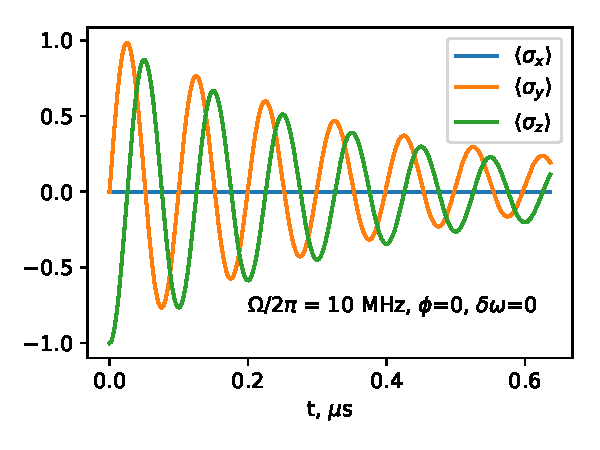
\includegraphics[width=0.6\textwidth]{images/Rabi_res.pdf}
	\caption[Динамика состояния кубита под действием внешнего поля в случае резонанса]{Динамика среднего состояния кубита под воздействием поля. Компоненты блоховского вектора $\{\braket{\sigma_x(t)}, \braket{\sigma_y(t)}, \braket{\sigma_z(t)}\}$ в явном виде заданы выражением $\eqref{eq: dyn_sol}$.}
	\label{img: Rabi_dyn_res}
\end{figure}

Отметим некоторые особенности полученного решения. Во-первых, частота Раби осцилляций определяется как $\Omega_r = \sqrt{\Omega^2-(\Gamma_1-2\gamma_\varphi)^2/16}$, и практически совпадает с $\Omega$ в случае достаточно сильного драйва. Затухание Раби-осцилляций определяется как $\Gamma_r = \frac{1}{4}\left(2 \gamma _{\varphi }+3 \Gamma _1\right) = \left(\Gamma_1 + \Gamma_2\right)/2$. Этот результат качественно объясняется тем, что примерно половину времени кубит проводит на экваторе сферы Блоха, где он существенно подвержен влиянию дефазировки, а другую половину кубит имеет положительную проекцию на ось $z$, и соответственно, подвержен влиянию затухания.
В случае $\delta\omega \ne 0$ окончательный ответ еще более громоздкий, поэтому мы не приводим уравнения, описывающие динамику в этом более общем случае. Динамика кубита при ненулевой отстройке изображена на~Рис.~\ref{img: Rabi_dyn_det} и \ref{img: Bloch_Rabi_dyn_det}. Заметим, что общий характер колебаний остается примерно таким же, что и в случае $\delta\omega=0$, однако, заметно меняется конечное состояние кубита, в котором он оказываеся после осцилляций - стационарное состояние. Получим явное выраджение, описывающее стационарное состояние кубита.
\begin{figure}[t]
	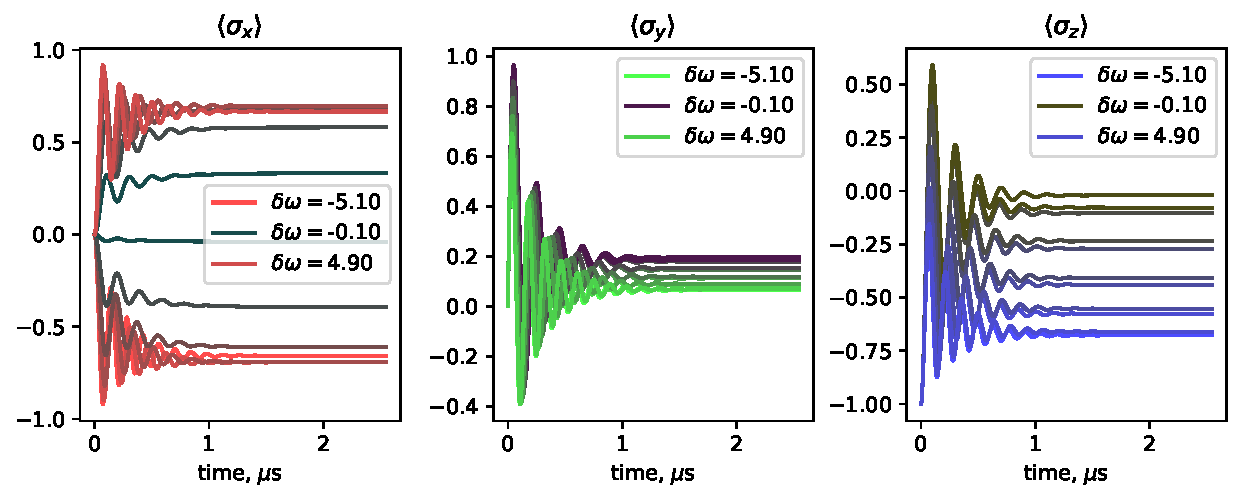
\includegraphics[width=0.98\textwidth]{images/Rabi_det_2.pdf}
	\caption[Динамика состояния кубита под действием внешнего поля: случай ненулевой отстройки]{Динамика компонент блоховского вектора $\vec{\sigma}(t)$ для $\Gamma_1=0.5, \gamma_\varphi=0.1, \Omega = 10$~МГц. Линии на каждом из графиков соответствуют значениям $\delta\omega=[-5.1,4.9]$~МГц }
	\label{img: Rabi_dyn_det}
\end{figure}
\begin{figure}[h]
	\centering
	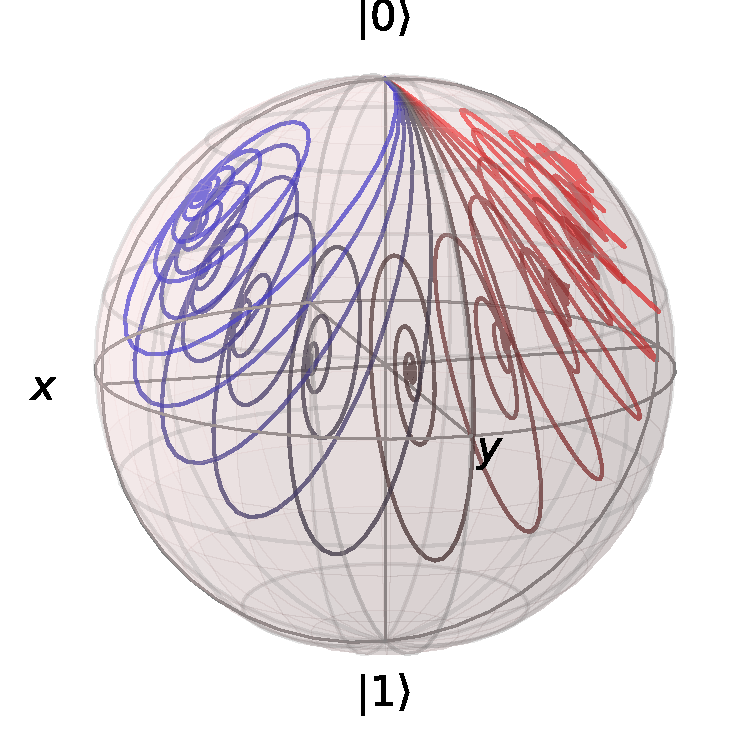
\includegraphics[width=0.65\textwidth]{images/Bloch_rabi_det.pdf}
	\caption[Динамика состояния кубита под действием внешнего поля на сфере Блоха]{Динамика состояния кубита при ненулевой отстройке внешнего драйва, изображенная на сфере Блоха. Кривые построены при тех же параметрах, которые использованы для Рис. \ref{img: Rabi_dyn_det}.}
	\label{img: Bloch_Rabi_dyn_det}
\end{figure}
\subsubsection{Стационарное решение уравнений Блоха}
Поскольку кубит постоянно взаимодействует с полем, время от времени обмениваясь энергией или информацией с внешней средой, то можно предположить, что временная динамика матрицы плотности, которая, строго говоря, описывает распределение эволюций одинаковых систем, через достаточно долгое время придет к некоторому стационарному значению $\vec{\sigma}_{st}$. Это легко проверить, положив в уравнениях \eqref{eq: Bloch}  $\dot{\vec{\sigma}}(t)=0$, что делает дифференциальные уравнения алгебраическими. Полагая $\varphi=0$ (что задает вращение вокруг оси $x$) и решая уравнения относительно компонент блоховского вектора, находим:
\begin{multline}
\rho_{x} = \frac{4 \Gamma_{1} \Omega \delta\omega}{4 \Gamma_{1} \delta\omega^{2} + \Gamma_{1} \left(\Gamma_{1} + 2 \gamma_{\varphi}\right)^{2} + 2 \Omega^{2} \left(\Gamma_{1} + 2 \gamma_{\varphi}\right)},\\\rho_{y} = \frac{2 \Gamma_{1} \Omega \left(\Gamma_{1} + 2 \gamma_{\varphi}\right)}{4 \Gamma_{1} \delta\omega^{2} + \Gamma_{1} \left(\Gamma_{1} + 2 \gamma_{\varphi}\right)^{2} + 2 \Omega^{2} \left(\Gamma_{1} + 2 \gamma_{\varphi}\right)},\\ \rho_{z} = - \frac{\Gamma_{1} \left(4 \delta\omega^{2} + \left(\Gamma_{1} + 2 \gamma_{\varphi}\right)^{2}\right)}{4 \Gamma_{1} \delta\omega^{2} + \Gamma_{1} \left(\Gamma_{1} + 2 \gamma_{\varphi}\right)^{2} + 2 \Omega^{2} \left(\Gamma_{1} + 2 \gamma_{\varphi}\right)},
\label{eq: stat_sol}
\end{multline}
где введено обозначение $\delta\omega=\omega_d-\omega_q$.
\begin{figure}[h]
	{ \raggedleft
		\hfill
		\def\svgwidth{2.5in}
		\fontsize{19pt}{19pt}\selectfont
		\subbottom[\label{img: bloch_stat1}]{%
			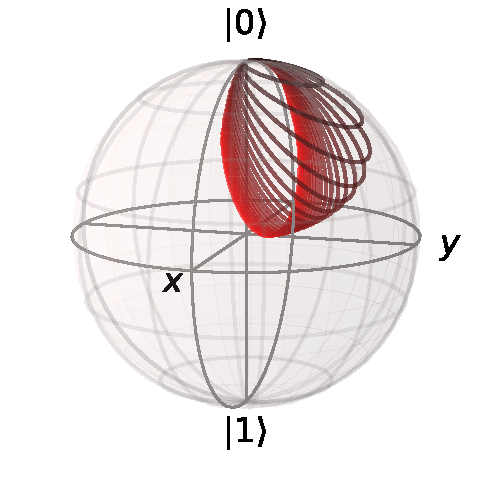
\includegraphics{images/bloch_stat1.pdf}}
		\hfill
		\def\svgwidth{2.5in}
		\subbottom[\label{img: bst2}]{%
			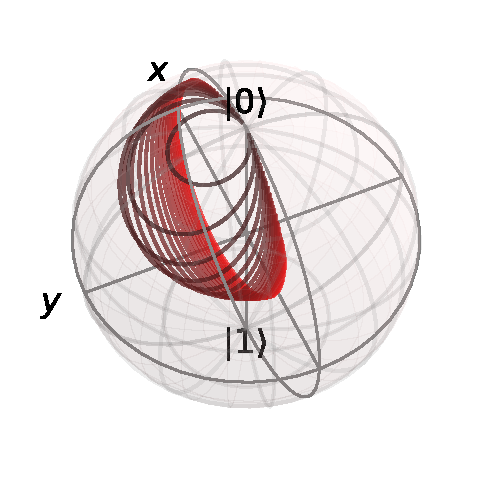
\includegraphics{images/bloch_stat2.pdf}}
		
		\hfill
	}
	\caption[Стационарное состояние кубита, вращаемого электромагнитным полем.]{Стационарное состояние \eqref{eq: stat_sol} кубита под воздействием поля, изображенное на сфере Блоха. Различные линии соответствуют значениям $\Omega=[0,10]$, $\Gamma_1=2, \gamma_\varphi=0 $~МГц. Каждая линия соответствуют изменению $\delta\omega=[-10,10]$~МГц. Панели а) и б) изображают одни и те же линии под различными ракурсами. Отметим, что эти линии образованы множеством точек, к которым приходит кубит после динамики, изображенной на~Рис. \ref{img: Bloch_Rabi_dyn_det} \label{img: bloch_stat}}
	
\end{figure}
Стационарные состояние в зависимости от параметров $\Omega, \Gamma_1, \gamma_\varphi$ изображено на Рис.~\ref{img: bloch_stat}. В случае $\Omega\!\ll\!\Gamma_1$ стационарное состояние приближено к состоянию $\ket{0}$, поскольку поле достаточно слабое для эффективного возуждения кубита. В случае $\Omega\!\gg\!\Gamma_1$ стационарное состояние приближено к смешанному состоянию, но имеет ненулевую проекцию на экваториальную плоскость. Рассчитаем эластичную часть излучения кубита в стационарном состоянии
\subsubsection{Эластичное рассеяние}
Поскольку нас интересует сигнал, рассеянный кубитом назад, то необходимо выразить компоненту поля, соответствующую отрицательной частоте, то есть, соотвествующую оператору $\langle\hat{\sigma}_- \rangle$. Используя решения \eqref{eq: stat_sol} и возвращаясь в лабораторную систему отчета, получим:
\begin{equation}
\braket{\hat{\sigma}_-} = \frac{1}{2}\left(\rho_x-i\rho_y\right) = -\frac{\Omega/\Gamma_2}{1+(\delta\omega/\Gamma_2)^2+\Omega^2/\Gamma_1\Gamma_2}\left(1-i\frac{\delta\omega}{\Gamma_2}\right)e^{-i\omega_d t},
\label{eq: stat_s-}
\end{equation} 
где $\Gamma_2 = \Gamma_1 + \gamma_\varphi/2$~ обозначает полную дефазировку кубита. Выражение \eqref{eq: stat_s-} уже может быть подставлено в \eqref{eq: r_derived}, однако, перед тем как сделать это, необходимо рассмотреть явную связь между излучательной релаксацией $\Gamma_1$ кубита в линию и квантовыми флуктуациями электромагнитного поля в линии, вызывающими эту релаксацию. В случае емкостной связи к зарядовому кубиту (или к трансмону) он чувствителен к флуктуациям напряжения в линии, и поскольку кубит подключен к двум полубесконечным линиям с полным импедансом $Z/2$, спектральную плотность флуктуаций напряжения можно записать в виде:
\begin{equation}
S_{V}(\omega_q>0)=\hbar \omega_q Z
\end{equation}
Согласно золотому правилу Ферми, релаксация в линию определяется \cite{nazarov2002quantum} как:
\begin{equation}
\Gamma_1 = \frac{|\!\braket{g|H_{int}|e}\!|^2}{V_0^2\hbar^2}S_V(\omega_q) = \frac{\omega_q Z}{\hbar}(\beta \langle{g|\hat{q}|e}\rangle|)^2 = \frac{\omega_q Z \mu^2}{\hbar}, 
\end{equation}
где введен дипольный момент кубита $\mu=\hbar\Omega/V_0$.
С учетом этих выражений, \eqref{eq: r_derived} принимает окончательный вид:
\begin{equation}
r = i\frac{\Gamma_1}{\Omega}\braket{\hat{\sigma}_-}e^{i\omega_d t} = \frac{\Gamma_1}{2\Gamma_2}\frac{1+i\delta\omega/\Gamma_2}{1+(\delta\omega/\Gamma_2)^2+\Omega^2/(\Gamma_1\Gamma_2)}
\label{eq: refl}
\end{equation}
Несложно показать, что это выражение справедливо как для различных типов кубитов, так и для различного способа связи с линией. Завичимость коэффициента отражения от $\Omega$ и $\delta\omega$ приведена на рисунке \ref{fig: refl}. При $\Omega\ll\sqrt{\Gamma_1\Gamma_2\vphantom{^2}}$ частотная зависимость $r$ имеет лоренцевскую форму с шириной линии $2\Gamma_2\approx\Gamma_1$. При увеличении $\Omega$ проявляется нелинейность кубита, и эффективность отражения падает, а форма линии значительно отклоняется от лоренцевской. Это также хорошо иллюстрируется с помощью изображения $r$ на комплексной плоскости. 

Рассмотрев стационарное излучение, необходимо вспомнить, что описание кубита при помощи матрицы плотности, находимой при помощи основного квантового уравнения, носит статистический характер. В динамике одиночной системы даже в стационарном состоянии происходит взаимодействие с электромагнитным полем, в результате которого возникают флуктуации измеряемых величин, например, напряжения в линии. Поэтому ясно, что какая-то часть сигнала излучается стохастически и не может быть когерентной, но должна проявляться в полном спектре излучения двухуровневой системы. Опишем, как происходит некогерентное (неэластичное) рассеяние волны на кубите, для чего нам потребуется рассчитать флуктуации поля, излучаемого кубитом в стационарном состоянии \eqref{eq: stat_sol}, а затем с использованием этих решений вывести соотношения для некогерентного сигнала, излучаемого кубитом.
\begin{figure}[ht]
	\centering
	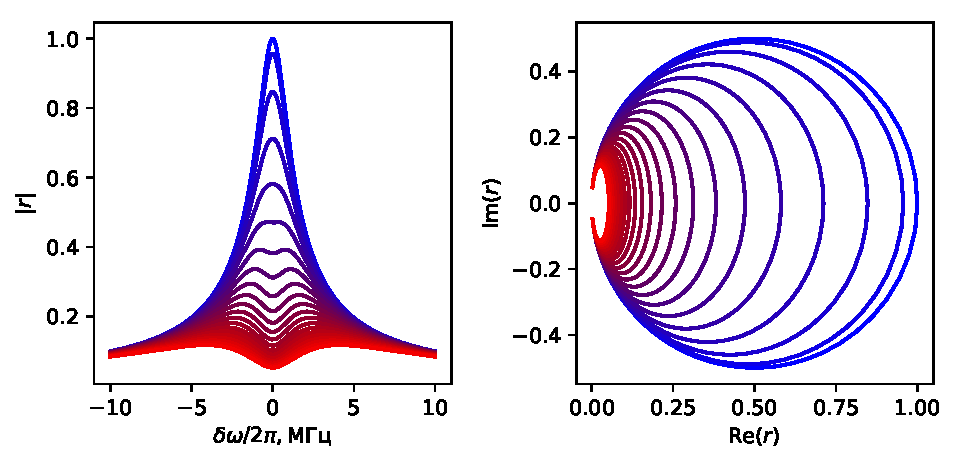
\includegraphics[width=0.9\textwidth]{relf.pdf}
	\caption[Коэффициент отражения в стационарном состоянии]{Стационарный коэффициент отражения непрерывной волны на частоте $\omega_q+\delta\omega$, направляемой на кубит. Слева: Зависимость $|r|(\delta\omega)$, где $\delta\omega/2\pi=[-10,10]$~МГц. Различные линии соответствуют значениям $\Omega/2\pi=[0,6]$~МГц, для всех линий $\Gamma_1/2\pi=2$~МГц, $\gamma_\varphi/2\pi=0$~МГц. Справа: $r$ на комплексной плоскости для $\delta\omega/2\pi=[-20,20]$~МГц и для тех же значений параметров $\Omega,\Gamma_1,\gamma_\varphi$.  }
	\label{fig: refl}
\end{figure}
\subsubsection{Спектр некогерентного излучения}
Будем рассматривать комплексный оператор напряжения в линии $\hat{V}(t)$ как некоторый случайный стационарный процесс. К нему можно применить теорему Винера-Хинчина, которая устанавливает однозначную связь между автокорреляционной функцией процесса, которую можно записать в виде $\braket{\hat{V}^{+}(0)\hat{V}^{-}(\tau)}$, и спектральной плотностью процесса. Будем искать спектральную плотность в стационарном состоянии:  
\begin{equation}
S_{VV}(\omega) = \frac{1}{2\pi Z}\int\limits_{-\infty}^{\infty}\braket{\hat{V}^{+}(0)\hat{V}^{-}(\tau)}_{ss}e^{i\omega \tau}\,d\tau
\end{equation}
С учетом \eqref{eq: refl} для оператора напряжения в точке связи с кубитом $x=0$ можно получить выражение:
\begin{equation}
\hat{V}^{\pm}(t) = i\frac{\hbar\Gamma_1}{\mu}\hat{\sigma}_\mp(t)e^{\mp i\omega_d t},
\end{equation}
Необходимо отметить, что это выражение представляет частный случай общего результата, согласно которому, поле, излучаемое атомом в дипольном приближении на далекое расстояние, пропорционально операторам $\sigma_-$ и $\sigma_+$ (см. уравнение (10.A.16) в \cite{Scully}).
C учетом последнего равенства имеем:
\begin{equation}
S_{VV}(\omega) = \frac{\hbar\omega_q
	 \Gamma_1}{2\pi}\int\limits_{-\infty}^{\infty}\braket{\hat{\sigma}_{+}(0)\hat{\sigma}_{-}(\tau)}_{ss}e^{i(\omega-\omega_d) \tau}\,d\tau.
\label{eq: SVV_sigmas}
\end{equation}
Операторы $\hat{\sigma}_+$ и $\hat{\sigma}_-$ можно представить при помощи введения операторов флуктуаций:
\begin{equation}
\hat{\sigma}_\pm(t)=\braket{\sigma_\pm}_{ss}+\Delta\hat{\sigma}_\pm(t),
\label{eq: fluct}
\end{equation}
при этом $\braket{\Delta\hat{\sigma}_\pm(t)}_{ss}\!=\!0$ по определению. С учетом этого представления, коррелятор преобразуется следующим образом:
\begin{equation}
\braket{\hat{\sigma}_{+}(0)\hat{\sigma}_{-}(\tau)}_{ss} = \braket{\hat{\sigma}_+(0)}_{ss} \braket{\hat{\sigma}_-(\tau)}_{ss} + \braket{\Delta\hat{\sigma}_{+}(0)\Delta\hat{\sigma}_{-}(\tau)}_{ss}.
\label{eq: correlator}
\end{equation} 
Таким образом, полная спектральная плотность излучения будет складываться из эластичной и неэластичной части:
\begin{equation}
S_{VV}(\omega) = S_{el}(\omega) + S_{in}(\omega)
\end{equation}
Первое слагаемое \eqref{eq: correlator} представляет собой произведение средних значений операторов в стационарном состоянии, и может быть посчитано с использованием \eqref{eq: stat_sol}, для простоты полагая $\delta\omega\!=\!0$:
\begin{equation}
\braket{\hat{\sigma}_\pm}_{ss} = \pm \frac{ie^{\mp i\varphi}}{2}\frac{\Gamma_1\Omega}{\Gamma_1\Gamma_2+\Omega^2}
\end{equation}
С использованием этого соотношения можно посчитать когерентную (эластичную) часть спектра:
\begin{align}
S_{el}(\omega) =& \frac{\hbar\omega_q
	\Gamma_1}{2\pi}\int\limits_{-\infty}^{\infty}\braket{\hat{\sigma}_{+}(0)}_{ss}\braket{\hat{\sigma}_{-}(\tau)}_{ss}e^{i(\omega-\omega_d) \tau}\,d\tau,\\
S_{el}(\omega) =& \frac{\hbar\omega_q\Gamma_1}{4}\frac{\Gamma_1^2\Omega^2}{\left(\Gamma_1\Gamma_2+\Omega^2\right)^2}\,\delta\!\left(\omega-\omega_d\right)
\end{align}
В случае слабого поля $\Omega^2\!\ll\!\Gamma_1\Gamma_2$ и $\Gamma_2\!=\!\Gamma_1/2$ имеем $S_{el}(\omega)\!=\!\delta\!\left(\omega-\omega_d\right)\cdot\hbar \omega_q\Omega^2/\Gamma_1$.  Расчет неэластичной части спектра 
\begin{equation}
S_{in}(\omega) = \frac{\hbar\omega_q
	\Gamma_1}{2\pi}\int\limits_{-\infty}^{\infty}\braket{\Delta\hat{\sigma}_{+}(0)\Delta\hat{\sigma}_{-}(\tau)}_{ss}e^{i(\omega-\omega_d) \tau}\,d\tau.
\label{eq: inelastic}
\end{equation}
требует вычисления кореллятора флуктуаций. 

Легко понять, что зависимость $\rho(t)$, получаемая из уравнений Блоха, сама по себе не дает корелляции, представляющие собой средние по состоянию значения произведения операторов в разные моменты времени. Для этого потребуется использовать так называемую \textit{квантовую регресионную теорему}, которая позволяет найти временную зависимость коррелляторов по известной динамике матрицы плотности. Кратко проиллюстрируем суть теоремы. Рассмотрим атом, взаимодействующий с некоторым резервуаром и описываемый матрицей плотности $\rho(t)$, которую в общем случае нельзя представить в виде произведения $\rho_a(t)\otimes\rho_R(t)$, так как атом и окружение могут быть запутаны. Рассмотрим марковское приближение, согласно которому, существует некоторый нулевой момент времени, в который состояния можно факторизовать: $\rho(0)=\rho_a(0)\otimes\rho_R(0)$ Зная начальное состояние $\rho(0)$, можно найти состояние системы в произвольный момент времени при помощи оператора эволюции: $\rho(t)=U(t)\rho(0)U^\dagger(t)$. Для того чтоб выделить состояние атома в момент времени $\tau$, необходимо взять частичный след по переменным резервуара: $\rho_a(\tau) = \tr_R(\rho(\tau))$. С учетом этого можно записать выражение для среднего значения оператора $\sigma_-$ в момент времени $\tau$ может быть записано как:
\begin{align}
\braket{\hat{\sigma}_-(\tau)} &=  \tr_a\left[\hat{\sigma}_-(0)\rho_a(\tau)\right],\\ \braket{\hat{\sigma}_-(\tau)} &=\tr_a\left[\hat{\sigma}_-(0)\tr_R\left(U(\tau)\left[\rho_a(0)\otimes\rho_R(0)\right]U^\dagger(\tau)\right)\right].
\label{eq: exp}
\end{align}
Аналогичным образом запишем среднее значение коррелятора:
\begin{multline}
\braket{\hat{\sigma}_+(0)\hat{\sigma}_-(\tau)} =\tr_a\left[\hat{\sigma}_+(0)\hat{\sigma}_-(0)\tr_R\left(U(\tau)\left[\rho_a(0)\otimes\rho_R(0)\right]U^\dagger(\tau)\right)\right]=\\=\tr_a\left[\hat{\sigma}_-(0)\tr_R\left(U(\tau)\left[\rho_a(0)\hat\sigma_+(0)\otimes\rho_R(0)\right]U^\dagger(\tau)\right)\right],
\label{eq: corr}
\end{multline}
где в последнем равенстве использованы свойства частичного следа \cite{nielsen2002quantum}. Сравнивая выражения \eqref{eq: exp} и \eqref{eq: corr}, приходим к интересному выводу: для того, чтоб получить зависимость коррелятора $\braket{\hat{\sigma}_+(0)\hat{\sigma}_-(\tau)}$, достаточно использовать выражение $\braket{\hat{\sigma}_-(\tau)}$, но вместо начального состояния атома $\rho_a(0)$ необходимо подставить оператор $\rho_a(0)\hat{\sigma}_+$. Аналогичное справедливо и для оператора $\braket{\Delta\hat{\sigma}_+(0)\Delta\hat{\sigma}_-(\tau)}$. В более обобщенном смысле теорема утверждает, что если справедлива система уравнений, описывающее динамику средних некоторого полного набора операторов $\hat{A}_i$ и записываемая в векторно-матричной форме:
\begin{equation}
\frac{d\braket{\vec{A}(t)}}{dt} = \mathbf{M}\braket{\vec{A}(t)},
\end{equation}
то для произвольного оператора системы $\hat{O}(t)$ справедливо также:
\begin{equation}
\frac{d}{d\tau}\!\braket{\hat{O}(t)\vec{A}(t+\tau)} = \mathbf{M}\braket{\hat{O}(t)\vec{A}(t+\tau)}
\end{equation}
Для нахождения $\braket{\Delta\vec{\sigma}(\tau)}$ можно использовать решение уравнений Блоха \eqref{eq: Bloch}. Перепишем уравнения Блоха для нестационарной части излучения:
\begin{equation}
\braket{\Delta\dot{\vec{\sigma}}(\tau)} = \mathbf{M}\braket{\Delta\vec{\sigma}(\tau)} \rightarrow \braket{\Delta\vec{\sigma}(\tau)} = e^{\mathbf{M}\tau}\braket{\Delta\vec{\sigma}(0)} %=e^{\mathbf{M}\tau}\left(\vec{\sigma}_0-\braket{\vec{\sigma}}_{ss}\right).
\label{eq: bloch_delta}.
\end{equation}
Согласно квантовой регресионной теореме, для нахождения $\braket{\Delta\hat{\sigma}_+(0)\Delta\vec{\sigma}(\tau)}$ вместо $\braket{\Delta\vec{\sigma}(0)}$ нужно подставить в \eqref{eq: bloch_delta} начальное условие $\braket{\Delta\hat{\sigma}_+(0)\Delta\vec{\sigma}(0)}$, которое вычисляется c помощью \eqref{eq: fluct} и \eqref{eq: stat_sol} как: 
\begin{equation}
\braket{\Delta\hat{\sigma}_+(0)\Delta\vec{\sigma}(0)} = \braket{\hat{\sigma}_+\vec{\sigma}}_{ss} - \braket{\hat{\sigma}_+}_{ss}\braket{\vec{\sigma}}_{ss}=
\left[\begin{matrix}
\frac{\Omega ^2}{\Gamma_1 ^2+2 \gamma_\varphi  \Gamma_1 +2 \Omega ^2} \\
\frac{i \Omega ^2 \left(-\Gamma_1 ^2+2 \gamma_\varphi  \Gamma_1 +2 \Omega ^2\right)}{\left(\Gamma_1 ^2+2 \gamma_\varphi  \Gamma_1 +2 \Omega ^2\right)^2} \\
-\frac{2 i \Gamma_1  \Omega ^3}{\left(\Gamma_1 ^2+2 \gamma_\varphi  \Gamma_1 +2 \Omega ^2\right)^2} 
\end{matrix}\right]
\end{equation}
после чего из \eqref{eq: bloch_delta} получаем:
\begin{multline}
\braket{\Delta\hat{\sigma}_+(0)\Delta\hat{\sigma}_-(\tau)}_{ss} = \frac{\Omega ^2}{2 \left(2 \gamma_\varphi  \Gamma_1 +\Gamma_1 ^2+2
	\Omega ^2\right)} \Bigg[e^{-\frac{1}{2} t (2 \gamma_\varphi +\Gamma_1 )} + e^{-\frac{1}{4} t (2 \gamma_\varphi +3 \Gamma_1 )} \cdot \\ \cdot \left( \frac{2 \gamma_\varphi  \Gamma_1 -\Gamma_1 ^2+2 \Omega ^2}{2 \gamma_\varphi  \Gamma_1 +\Gamma_1 ^2+2
	\Omega ^2}
		\cos \Omega _g t - \frac{ 2 \Omega ^2 (2 \gamma_\varphi -5 \Gamma_1 )+\Gamma_1  (\Gamma_1 -2 \gamma_\varphi )^2}{4\Omega_g\left(2 \gamma_\varphi  \Gamma_1 +\Gamma_1 ^2+2
			\Omega ^2\right)} \sin \Omega _g  t \right)\Bigg].
\label{eq: Corr(t)}
\end{multline}
Выражение \eqref{eq: Corr(t)} получено без каких-либо приближений. Дальнейшее вычисление спектральной плотности сводится к преобразованию Фурье и приводит к достаточно громоздким выражениям, поэтому оно будет опущено. Для частного случая сильного драйва $4\Omega \gg \Gamma_1, \gamma_\varphi$ получается выражение:
\begin{equation}
S_{in}(\delta\omega) = \frac{1}{2\pi}\frac{\hbar \omega_q\Gamma_1}{4}\Big(\frac{\gamma_s}{(\delta\omega+\Omega)^2+\gamma_s^2}+\frac{2\gamma_c}{\delta\omega^2+\gamma_c^2}+\frac{\gamma_s}{(\delta\omega-\Omega)^2+\gamma_s^2}\Big),
\label{eq: mollow}
\end{equation}
где введены обозначения $\gamma_c = \Gamma_1/2 + \gamma_\varphi = \Gamma_2$, $\gamma_s = 3\Gamma_1/4 + \gamma_\varphi/4 = (\Gamma_1 + \Gamma_2)/2$.
Отличительной особенностью данного спектра явяется наличие боковых пиков при $\delta\omega = \pm \Omega$. Отметим также, что в отличие от спектральной плотности эластичной части излучения, которая максимальна при $\Omega = \sqrt{\Gamma_1 \Gamma_2}$ и далее уменьшается при увеличении $\Omega$, спектральная плотность неэластичной части возрастает от нуля при $\Omega = 0 $ до некоторого максимального значения. Поскольку спектр \eqref{eq: mollow} состоит из трех лоренцевских пиков, достаточно разделяющихся при $\Omega \gg \Gamma_1$, то полная мощность, рассеиваемая кубитом, равна $\hbar \omega_q \Gamma_1/2$. Этот ответ допускает наглядную качественную интерпретацию. Сильное поле не взаимодействует с кубитом когерентно, но вызывает квантово-механические скачки с основного на возбужденный уровень и обратно со средней частотой $\Gamma_1$. Таким образом, эффективно кубит излучает мощность, соответствующую половине энергии фотона, которая излучается за время релаксации. Спектр некогерентного излучения изображен на Рис.~\ref{fig: Mollow}.
\begin{figure}[th]
	\centering
	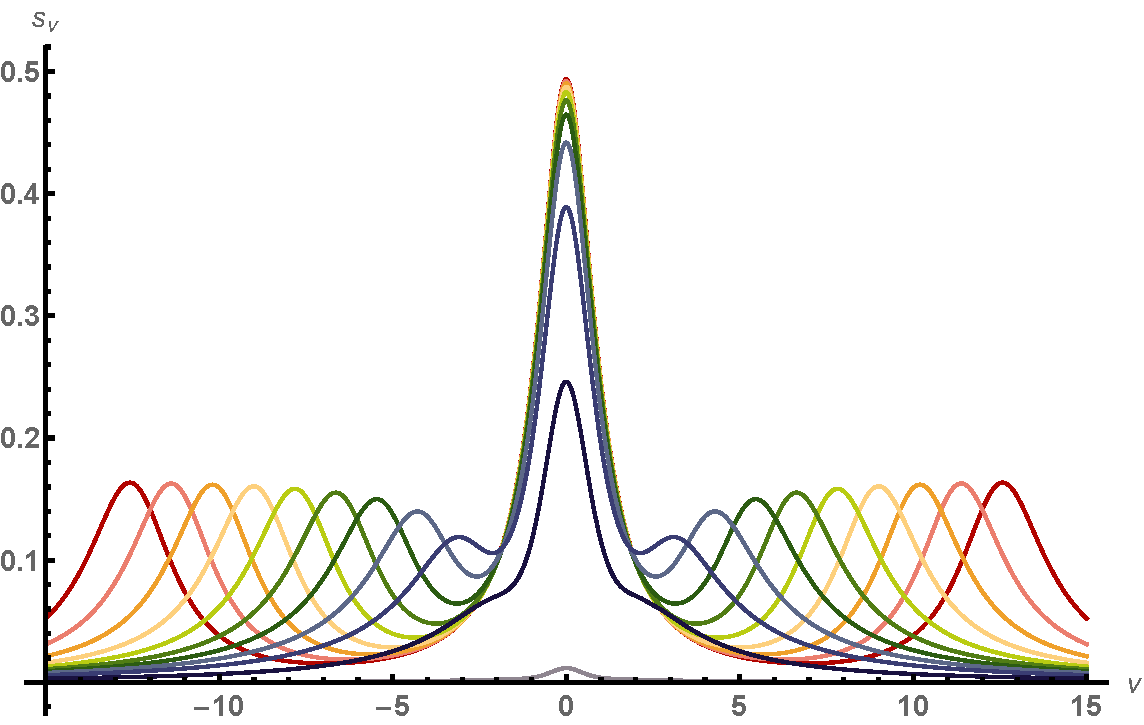
\includegraphics[width=0.7\textwidth]{images/Mollow.pdf}
	\caption[Спектр резонансной флуоресценции.]{Спектр неэластичного рассеяния для $\Gamma_1 = 2$ МГц, $\gamma_\varphi=0$, $\Omega = [1.5, 12.5]$~МГц. }
	\label{fig: Mollow}
\end{figure}
%где в последнем равенстве использовано начальное условие $\vec{\sigma}_0 = \{0,0,\!-\!1\}$. В результате искомый кореллятор находится как
%\begin{equation}
%\braket{\Delta\hat{\sigma}_-(0)\Delta\hat{\sigma}_+(0)} = \frac{1}{2} \left(e^{-\frac{1}{2} \tau (2 \gamma +\Gamma )}+\frac{\Omega _g e^{-\frac{1}{4} \tau (2 \gamma +3 \Gamma )} \left(\left(4 \gamma ^2
%	\Gamma -i \Gamma  \Omega  (6 \gamma +\Gamma )+4 \gamma  \Omega ^2-\Gamma ^3\right) \sinh \left(t \Omega _g \right)-4 \Omega _g \left(2 \gamma  \Gamma
%	+\Gamma ^2-i \Gamma  \Omega +2 \Omega ^2\right) \cosh \left(t \Omega _g \right)\right)}{4 \Gamma  (2 \gamma +\Gamma )+8 \Omega ^2}\right)
%\end{equation}

Мы рассмотрели основные эффекты, возникающие при взаимодействии двухуровневой системы (сверхпроводникового кубита), сильно связанной с волноводом, и внешнего классического поля, распространяющегося в волноводе (проходной линии). Можно отметить, что даже в таком простом случае физика происходящих явлений весьма нетривиальна. Однако, в главе \ref{ch: Quant} показано, что сверхпроводниковые кубиты не являются двухуровневыми системами: во многих случаях необходимо учитывать третий и следующие уровни энергии. В квантовой оптике, взаимодействие света с трехуровневой системой порождает целый ряд явлений, таких как электромагнитно-индуцированная прозрачность, когерентный захват заселенности и другие. Опишем некоторые из эффектов, возникающие в трехуровневых системах.

\subsection{Квантовооптические эффекты в трёхуровневых системах}
СКЦ, как и любая квантовая система, имеет большое количество собственных энергетических уровней. Если энергии третьего (второго возбужденного) уровня СКЦ настолько велики, что частоты переходов с первых двух уровней превышают частоты внешнего электромагнитного поля, с которым взаимодействует система, то справедливо двухуровневое приближение. Однако во многих случаях это не так, и необходимо учитывать наличие третьего уровня. 

Как и для <<природных>> атомов химических элементов, для сверхпроводниковых цепей справедливы правила отбора: в дипольном приближении, запрещены переходы между теми состояниями, волновые функции которых имеют одинаковую симметрию. Так, например, для трансмонов, структура волновых функций которых достаточно близка к гармоническому осциллятору, запрещены переходы $\ket{0}\rightarrow\ket{2}$ и обратно. На основе правил отбора можно выделить несколько типов трехуровневых систем, схематично изображенных на Рис.~\ref{fig: 3LS_class}.  
\begin{figure}[th]
	\centering
	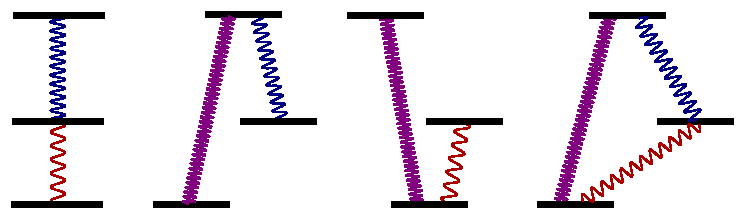
\includegraphics[width=0.8\textwidth]{images/3Ls_V_Lbd_ladder.pdf}
	\caption[Классификация трехуровневых систем по разрешенности переходов.]{Классификация трехуровневых систем, порождаемая правилами отбора; слева направо --- схематичное изображение $\Xi$-, $\Lambda$-, $V$-, и $\Delta$-системы, соответственно. Волнистые линии связывают пары уровней, переход между которыми разрешен в дипольном приближении.}
	\label{fig: 3LS_class}
\end{figure}
Конфигурации уровней под названием $\Xi$-система (или лестничная система), $\Lambda$-система и $V$-система часто возникают в природных атомах, тогда как $\Delta$-система достаточно нехарактерна для них и поэтому достаточно слабо изучена экспериментально. Она может быть реализована только при помощи киральных молекул, а также в искусственных оптических системах на основе СКЦ. По аналогии с двухуровневой системой, можно записать гамильтониан, описывающий $\Lambda$-систему с частотами переходов $\omega_{02}$~и~$\omega_{12}$, которая взаимодействует с двумя электромагнитными модами $\omega^d_{12}$~и~$\omega^d_{02}$:
\begin{equation}
H = \left[\begin{matrix}\delta_{02} - \omega^{d}_{02} & 0 & \Omega_{02} \cos{\left (\omega^{d}_{02} t \right )}\\0 & \delta_{12} - \omega^{d}_{12} & \Omega_{12} \cos{\left (\omega^{d}_{12} t \right )}\\\Omega_{02} \cos{\left (\omega^{d}_{02} t \right )} & \Omega_{12} \cos{\left (\omega^{d}_{12} t \right )} & 0\end{matrix}\right],
\end{equation}
где введено обозначение $\delta_{12} = \omega^d_{12}-\omega_{12}$, $\delta_{02}$ --- аналогично. Переходя во вращающуюся систему отсчета и используя приближения вращающейся волны, этот гамильтониан можно привести к виду:
\begin{equation}
H_{RW\!A}=\left[\begin{matrix}\delta_{02} & 0 & \frac{\Omega_{02}}{2}\\0 & \delta_{12} & \frac{\Omega_{12}}{2}\\\frac{\Omega_{02}}{2} & \frac{\Omega_{12}}{2} & 0\end{matrix}\right]
\label{eq: 3LS_Hrwa}
\end{equation}
Оператор плотности, описывающий трехуровневую систему, можно записать стандарным образом:
\begin{equation}
\rho = \left[\begin{matrix}- \rho_{11} - \rho_{22} + 1 & i \rho^{i}_{01} + \rho^{r}_{01} & i \rho^{i}_{02} + \rho^{r}_{02}\\- i \rho^{i}_{01} + \rho^{r}_{01} & \rho_{11} & i \rho^{i}_{12} + \rho^{r}_{12}\\- i \rho^{i}_{02} + \rho^{r}_{02} & - i \rho^{i}_{12} + \rho^{r}_{12} & \rho_{22}\end{matrix}\right]
\end{equation}
Влияние диссипации и декогеренции на динамику системы описывается стандартным образом, см. \ref{sec:Lind}; отметим, что в трехуровневой системе скорости релаксации $ \Gamma_{01}, \Gamma_{02}, \Gamma_{12}$ и дефазировки $\gamma_{02}, \gamma_{12}$~и~$\gamma_{01}$ в общем случае независимы и могут значительно отличаться. Линдбладовский член имеет следующий вид:
\begin{equation}
\left[\begin{matrix}\Gamma_{02} r_{22} & - \gamma_{01} \left(i r^{i}_{01} + r^{r}_{01}\right) & - \frac{\left(i r^{i}_{02} + r^{r}_{02}\right) \left(\Gamma_{02} + \Gamma_{12} + 2\gamma_{02}\right)}{2}\\ \gamma_{01} \left(i r^{i}_{01} - r^{r}_{01}\right) & \Gamma_{12} r_{22} & - \frac{\left(i r^{i}_{12} + r^{r}_{12}\right) \left(\Gamma_{02} + \Gamma_{12} + 2\gamma_{12}\right)}{2}\\\frac{\left(i r^{i}_{02} - r^{r}_{02}\right) \left(\Gamma_{02} + \Gamma_{12} + 2\gamma_{02}\right)}{2} & \frac{\left(i r^{i}_{12} - r^{r}_{12}\right) \left(\Gamma_{02} + \Gamma_{12} + 2\gamma_{12}\right)}{2} & - r_{22} \left(\Gamma_{02} + \Gamma_{12}\right)\end{matrix}\right]
\label{eq: Lindblad_3ls}
\end{equation}

Рассмотрим случай, когда амплитуда $\Omega_{12}$ достаточно большая по сравнению со всеми константами релаксации и дефазировки и $\delta_{12}=0$. Это поле будет связывать состояния $\ket{1}$ и $\ket{2}$, и формировать новые собственные состояния системы ---  так называемые \textit{одетые состояния} $\left(\ket{1} \pm \ket{2}\right)/\sqrt{2}$ c энергиями $\pm\Omega_{12}/2$. Предположим теперь, что амплитуда поля $\Omega_{02}$ невелика, и поле носит характер пробного сигнала, не меняя при этом структуру уровней системы. Как мы увидим далее, это пробное поле позволяет непосредственно увидеть одетые уровни, созданные сильной накачкой перехода 1-2. Для нахождения стационарного состояния системы необходимо решить уравнение \eqref{eq: QLiouv} с гамильтонианом \eqref{eq: 3LS_Hrwa},  диссипатором \eqref{eq: Lindblad_3ls}, а также зануленной левой частью.
\subsection{Обзор последних достижений}

           % Глава 1
\chapter{Потоковые кубиты в волноводе: изготовление и характеризация}

В этой главе излагаются результаты измерений одиночных сверхпроводниковых потоковых кубитов, сильно связанных с волноводом --- микроволновой копланарной проходной линией на чипе. Для проведения экспериментов по нелинейному рассеянию света требовалось изготовить <<искусственный атом>> --- двухуровневую систему, сильно связанную с внешним микроволновым излучением, свободно распространяющимся в пространстве. Описывается подход к проектированию образцов, в частности, подбору параметров, которые позволяют достичь режима сильной связи. Описывается процесс изготовления образцов с использованием методов электронной и лазерной литографии. Затем излагаются экспериментальные условия, необходимые для изучения квантовой динамики такого кубита, а также процесс сборки измерительной схемы внутри криостата растворения. Приводятся результаты измерений коэффициента отражения резонансного микроволнового сигнала, а также результаты измерения спектра неэластичного рассеяния и излучение при эволюции кубита под действием внешнего поля. При помощи теоретической модели, подгоняемой под результаты измерений, вычисляются частота кубита и скорости релаксации в линию и дефазировки кубита. 

\section{Проектирование и изготовление образцов}
Первоначальный этап создания СКЦ --- проектирование дизайна. При проектировании необходимо учитывать, что уровни энергии квантовой электрической цепи, которая впоследствии будет сфабрикована на чипе, должны попасть в рабочий частотный диапазон измерительной схемы --- примерно от 2 до 12 ГГц. Зачастую для оптимальной работы схемы необходимо выдержать частоту с гораздо большей точностью: с разбросом не более 1-2 ГГц. Поэтому необходимо использовать дизайны, свободные от паразитных емкостей и индуктивностей отдельных структур, а при невозможности полностью избавиться от них провести правильный учет таких нежелательных элементов. Еще более важно учитывать физические ограничения на ряд параметров, которые накладывают реальные возможности оборудования, использующегося для изготовления кубитов. Для того, чтоб хорошо представлять эти ограничения, опишем методики изготовления СКЦ на чипе. 
\subsection{Фабрикационные ограничения}
Любая СКЦ представляет из себя некоторое количество островков сверхпроводящих плёнок, напыленных на диэлектрическую подложку (чип) из кремния или сапфира. Островки образуют различные электрические элементы --- джозефсоновские переходы, сосредоточенные или распределенные емкости и индуктивности. Общий размер чипа не может быть слишком большим по причине паразитных объемных мод в кремниевой пластинке. Частота нижней моды при продольном размере подложки 1 см составляет $\nu\approx2c/(\sqrt{\varepsilon}\lambda)\approx17$~ГГц. При б\'{о}льших продольных размерах частоты объемных мод могут попасть в диапазон измерений и создавать значительные помехи при измерении кубитов. На поверхности чипа формируются как кубиты, так и вспомогательные структуры. Как правило, все вспомогательные структуры достаточно велики, и их можно сформировать с помощью фотолитографии (масочной или безмасковой),которая позволяет сформировать структуры с размерами не менее 1-2 мкм. Сюда относятся: большие (сотни мкм) и по возможности односвязные острова, которые при помещении чипа в держатель будут заземлены; острова копланарных или микрополосковых резонаторов и проходных линий (волноводов) с поперечными размерами 10-20 мкм; контактные площадки для подключения линий с размерами порядка сотен мкм; отверстия-ловушки для сверхпроводящих вихрей порядка 10 мкм. Все эти структуры обычно напыляются через общую маску, и таким образом, формируются за один процесс литографии. 

Острова, формирующие кубиты, могут быть также достаточно большими (10-100 мкм), но размеры необходимо контролировать более точно, чем во вспомогательных структурах, поскольку от этого зависят частоты кубитов. Практически в любом кубите требуется сформировать джозефсоновские переходы между островами. Размеры переходов принципиально ограничены сразу несколькими факторами. Практически единственная хорошо отработанная методика изготовления переходов базируется на контролируемом формировании аморфного оксида алюминия на поверхности свеженапылённой либо очищенной в высоком вакууме алюминиевой пленки и последующего повторного напыления алюминия. Окисление происходит в атмосфере чистого кислорода с парциальным давлением 0.01-2 мБар, напускаемого в вакуумную камеру. Особенность этого окисления в том, что кислород перестает диффундировать в алюминий при очень малой толщине аморфной оксидной пленки (порядка 2-3 нм), что прекрасно подходит для формирования джозефсоновской связи с плотностями критического тока порядка $0.1-10$~мкA/мкм$^2$. В результате этого формируется джозефсоновский переход Al-AlOx-Al, и в качестве сверхпроводящего металла очень естественно используется тот же алюминий, хотя возможны и варианты, при которых оксид алюминия выращивается на пленках другого металла. По совпадению, аморфный оксид алюминия, сформированный \textit{in situ}, является достаточно чистым и содержит очень небольшое количество адсорбированных примесей и неоднородностей, которые могут связываться с кубитом. Тем не менее, известно, что переходах с размерами несколько мкм количество таких дефектов уже достаточно велико, и они отрицательно влияют на кубит, взаимодействуя с ним. Это одна из причин, по которой большие переходы не подходят для изготовления кубитов. 

Еще один фактор, ограничивающий площади переходов - джозефсоновская энергия. Для перехода размерами 1x1 мкм с плотностью критического тока 0.5 мкА/мкм$^2$ джозефсоновская энергия составляет $E_J\:=248$~ГГц, и при использовании такого перехода в кубитах, частота либо потоковая дисперсия кубитов, как правило, будет слишком большой. Это приводит к необходимости уменьшения площади джозефсоновских переходов до субмикронных размеров порядка сотен нм. Для контролируемого изготовления литографической маски с такими размерами необходима литография электронным лучом, разрешение которой может достигать 10 нм. Поэтому электронный литограф является одними из ключевых приборов для изготовления СКЦ и являются. 

Еще один важный момент заключается в том, что внутренняя емкость переходов практически не зависит от параметров окисления, так как толщина оксидного барьера практически одинакова даже для тех переходов, у которых $E_J$ различаются на порядок и более. Экспериментально известно, чтo у переходов Al-AlOx-Al размерами 100x100 нм емкость составляет $0.45$~фФ \cite{JJ_capacitance}. Поэтому переходы субмикронных и особенно микронных размеров неизбежно будут содержать значительную емкость, которая также может повлиять на энергии кубитов.
 
\subsection{Схема и дизайн кубитов}
В качестве атома было решено использовать потоковый кубит. Этот выбор определяется тем, что структура потенциальной (фазовой) энергии потокового кубита такова, что два нижних состояния $\ket{g}$ и $\ket{e}$ локализованы в двух близко расположенных и неглубоких потенциальных ямах, и высота барьера между этими ямами зависит от параметра $\alpha$, в частности, при $\alpha=0.5$ барьер исчезает полностью. Уровень $\ket{f}$ и следующие состояния лежат гораздо выше по энергии.  Это приводит к тому, что в точке вырождения по потоку $E_{ge} \sim 5$-$10$~ГГц, а $E_{ef} \approx 20$~ГГц, то есть, для генерируемых приборами управляющих импульсов длительностью более чем 1 нс влиянием верхних уровней на заселенности состояний $\ket{g}$ и $\ket{e}$ можно пренебречь. 
В качестве конкретной физической цепи, реализующей кубит, была выбрана схема потокового кубита с одним $\alpha$-переходом и тремя <<индуктивными>> переходами. По сравнению с более типичной схемой из трех джозефсоновских переходов, выбранная схема имеет как преимущества, так и недостатки. Перечислим их:

\begin{itemize}
	\item[$+$] В схеме с тремя переходами неизбежно возникает 4-й паразитный джозефсоновский переход, образуемый пересечением плёнок, формирующих основные переходы. Как правило, этот переход очень большой, индуктивность его очень мала и практически всегда его влиянием можно пренебречь. Тем не менее, схема с 4-мя переходами обладает симметрией по отношению к протеканию тока по пленкам и концептуально более правильная;
	\item[$+$] Зависимость крутизны уровней кубита по магнитному потоку от параметров схемы носит довольно сложный характер как в 3-переходном, так и в 4-переходном дизайне. Вдали от точки $\Phi=\Phi_0/2$ крутизна определяется суммарной индуктивностью больших переходов, и поэтому при равных размерах переходов чувствительность к потоковому шуму менее выражена именно для 4-переходного дизайна. 
	\item[$+$] В оптимальной точке $\Phi=\Phi_0/2$  зависимость энергии кубита определяется высотой барьера и резко зависит от $\alpha$ в обоих схемах. Однако, в 4-переходном дизайне есть возможность сделать <<индуктивные>> переходы несколько больше по площади, поэтому $\alpha$ несколько менее чувствительна к неточностям в площади сечения $\alpha$-перехода по отношению к расчетной.
	\item[$-$] Число степеней свободы в 4-переходном дизайне на единицу больше, что значительно замедляет численный расчет кубитов. 
\end{itemize}

Все вышеперечисленные преимущества вытекают из качественных соображений и в рамках данной работы их справедливость не проверялась какими-либо количественными расчетами или моделированием. Тем не менее, общая тенденция постепенного отказа от работы с потоковыми кубитами в пользу дизайнов типа вч-СКВИДа с большими индуктивностями также свидетельствует в пользу сделанного выбора. 

Принципиальная схема кубита, емкостно связанного с бесконечной копланарной линией, изображена на Рис. \ref{img: 4jj_flux_q}\subcaptionref*{img: 4jj_fluxQ_spectrum}. Отметим некоторые особенности данной схемы. Во-первых, связывающая емкость $C_c$  должна учитываться при расчете кубита, поскольку ёмкости джозефсоновских переходов по величине сопоставимы с емкостью связи. Во-вторых, бесконечные копланарные линии с волновым соспротивлением $Z_0=50$~Ом подключены с обеих сторон от кубита. Это изменит эффективное сопротивление, шум от которого вызывает релаксацию кубита : $Z=Z_0/2=25$~Ом, и это необходимо учитывать при расчете константы релакцации.
 
\begin{figure}[h]
	{ \centering
		\hfill
		\def\svgwidth{2.8in}
		\fontsize{18pt}{18pt}\selectfont
		\subbottom[List-of-Figures entry][\label{img: 4jj_fluxQ_scheme}]{%
			\input{images/4jj_flux_qubit_line_2.pdf_tex}}
		\hfill
		\subbottom[\label{img: 4jj_fluxQ_spectrum}]{%
			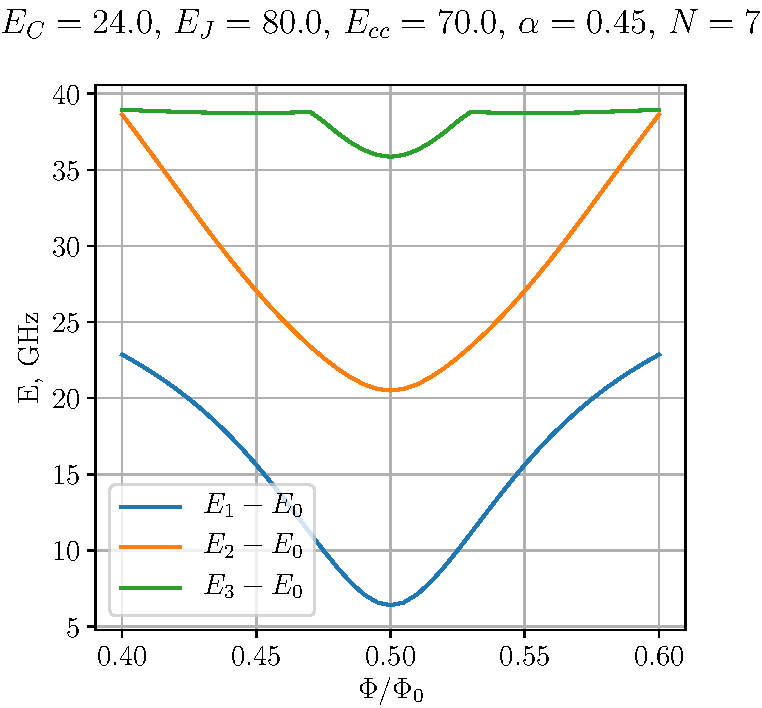
\includegraphics[width=0.55\textwidth]{images/4jj_qubit_spectra_side_coupled}}
		
		\hfill
	}
	\caption[Схема потокового кубита с четырьмя джозефсоновскими переходами и его спектр]{Потоковый кубит с 4 переходами: a) Эквивалентная схема кубита, связанного с волноводом.  б) Спектр кубита: энергии переходов из основного состояния в зависимости от внешнего потока через петлю для некоторых типичных значений параметров. Значения $E_C, E_J, E_{cc}$~приведены в ГГц. }
	\label{img: 4jj_flux_q}
\end{figure}

\begin{figure}[h]
	\centering
	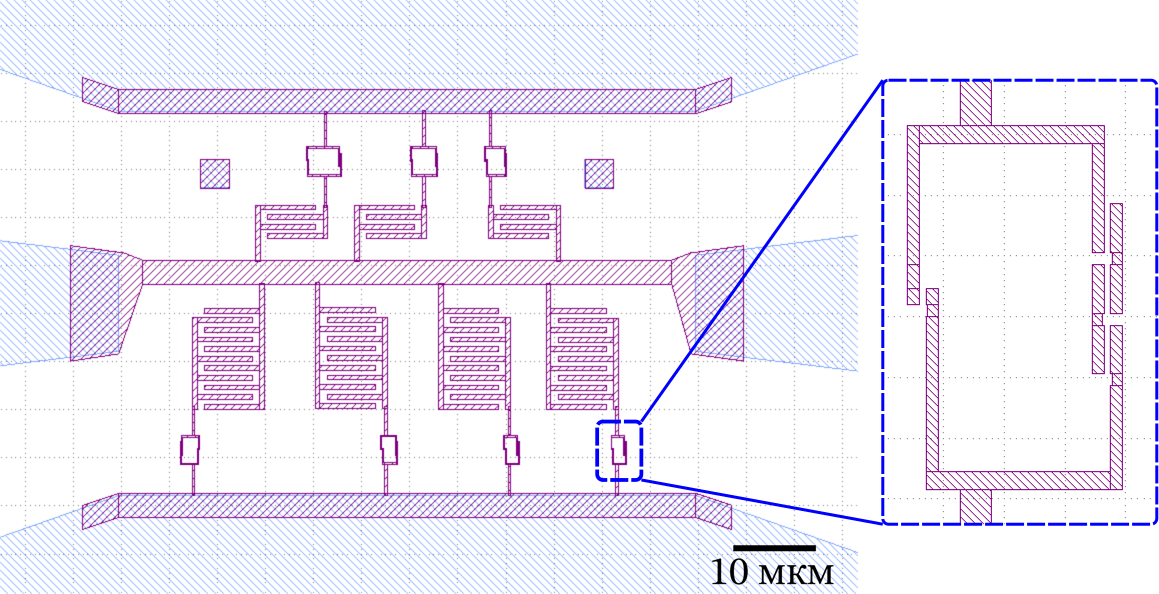
\includegraphics[width=1\textwidth]{images/fig_qubits_design.png}
	\caption{Дизайн потоковых кубитов, параллельно связанных с копланарной линией при помощи емкостей. Параметр $\alpha=0.36,0.45$, площади петель от 5 до 40 мкм$^2$, связывающие емкости $C_c=2.2,6.4$~фФ }
	\label{img: 4jj_side}
\end{figure} 
\begin{figure}[h]
	\centering
	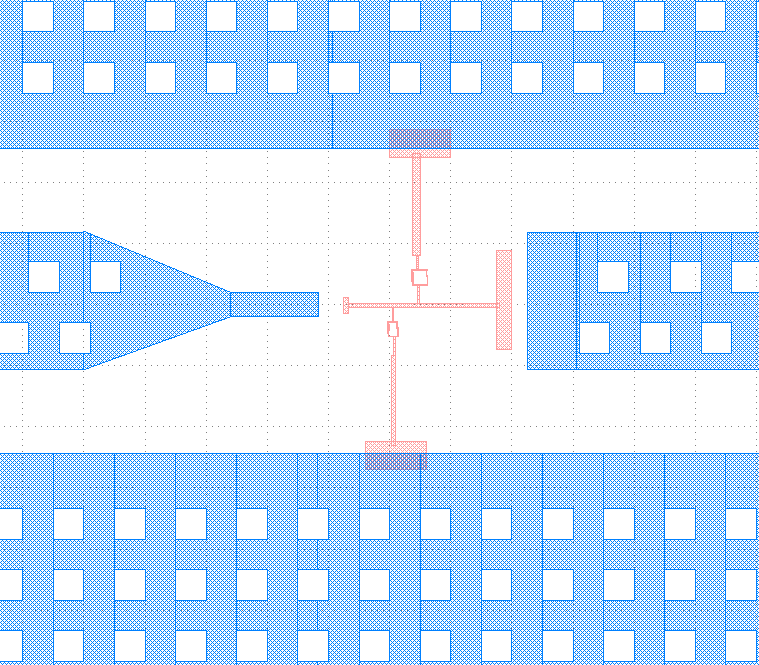
\includegraphics[width=0.6\textwidth]{images/SPS_design2.png}
	\caption{Дизайн 4-переходных потоковых кубитов, связанных с двумя полубесконечными копланарными линиями. Параметр $\alpha=0.4$, площади петель 14.2 и 21.2 мкм$^2$, связывающие емкости $C_{in}=0.24, C_{out} = 2.2 $~фФ }
	\label{fig: qubits_sps}
\end{figure} 
Для последующей фабрикации были рассчитаны и отрисованы дизайны экспериментальные образцов: дизайн на рис. \ref{fig: qubits_sps} реализует режим прямой связи (англ. \textit{direct coupling}), а дизайн образца на рис.
\ref{img: 4jj_side} --- режим параллельной связи (англ. \textit{side coupling}) кубита к излучению. Выбор схем не оказывает прямого влияния на процесс фабрикации кубитов. Остановимся на дизайне с параллельной связью. Спроектированный дизайн содержат кубиты с 4-мя джозефсоновскими переходами, три из которых имеют одинаковую площадь $200\times800$~нм, а еще один переход в $\alpha\approx0.4$ раз меньше остальных. Переходы будут формироваться при напылении через маску, повторяющую дизайн, под различными углами, примерно $\pm11^\circ$ Кубит связывается с электромагнитным полем, распространяющемся в копланарном волноводе, посредством связывающей емкости $C_c=2.2$ или $6.4$~фФ. Эта емкость фактически оказывается подключенной к земле через небольшое активное сопротивление $Z_0$ и поэтому оказывает шунтирующий эффект на $\alpha$-переход, необходимый для уменьшения чувствительности потокового кубита как к потоковым, так и зарядовым шумам. Более подробно, шунтирование~$\alpha$-перехода, добавляясь к внутренней емкости перехода $C_j=2$-$3$~фФ, уменьшает зарядовую энергию. Это приводит к тому, чтоб есть возможность уменьшить джозефсоновские энергии переходов, сохраняя при этом частоты кубитов. Это понижает чувствительность кубита к магнитному полю и, соответственнно, к шуму магнитного потока, что при прочих равных условиях может увеличить время когерентности. Влияние шунтирующей емкости на спектры 3-переходного потокового кубита отражено на Рис. \ref{fig: 3jj_spectra}. Также влияние емкостного шунта на потоковые кубиты детально исследовано в работе \cite{yan2016flux}, как теоретически, так и экспериментально. При существенно б$\acute{\text{о}}$льших значениях шунтирующей емкости порядка $50$ фФ кубит, фактически, становится слабо ангармоничным осциллятором с небольшими следами <<двухъямности>>, ангармонизм падает значительно ниже 1 ГГц. Это перспективно для достижения больших времен когерентности, но нежелательно для выполнения поставленных в диссертации задач. Для иллюстрации изложенных закономерностей, на рис. \ref{img: 4jj_flux_q}\subcaptionref*{img: 4jj_fluxQ_spectrum} приведены типичные зависимости энергии уровней от внешнего магнитного поля (спектры) кубитов для реалистичного набора параметров, полученные при помощи численной диагонализации полного гамильтониана в зарядовом базисе. В рабочем режиме частота кубита $\omega_0=E_e-E_g/\hbar$ должна находиться в пределах 2-10 ГГц, что обусловлено частотными диапазонами криогенных усилителей и изоляторов (подробнее об этом ниже).

Магнитное поле через кубиты обычно подается при помощи сверхпроводящего соленоида, который намотан на держатель и будет показан ниже. Однако, такой способ не может обеспечить индивидуальную перестройку частоты отдельных кубитов. Поэтому в ряде случаев полезно иметь возможность менять поток через потоковый кубит (или через СКВИД кубита-трансмона) при помощи дополнительной потоковой линии на чипе. Потоковая линия представляет собой копланарный волновод, который закорочен на землю вблизи той петли, поток в которой необходимо менять. Ток, текущий в потоковой линии, создает локальное магнитное поле, которое используется для перестройки магнитного потока. 

\begin{figure}[htb]\center
	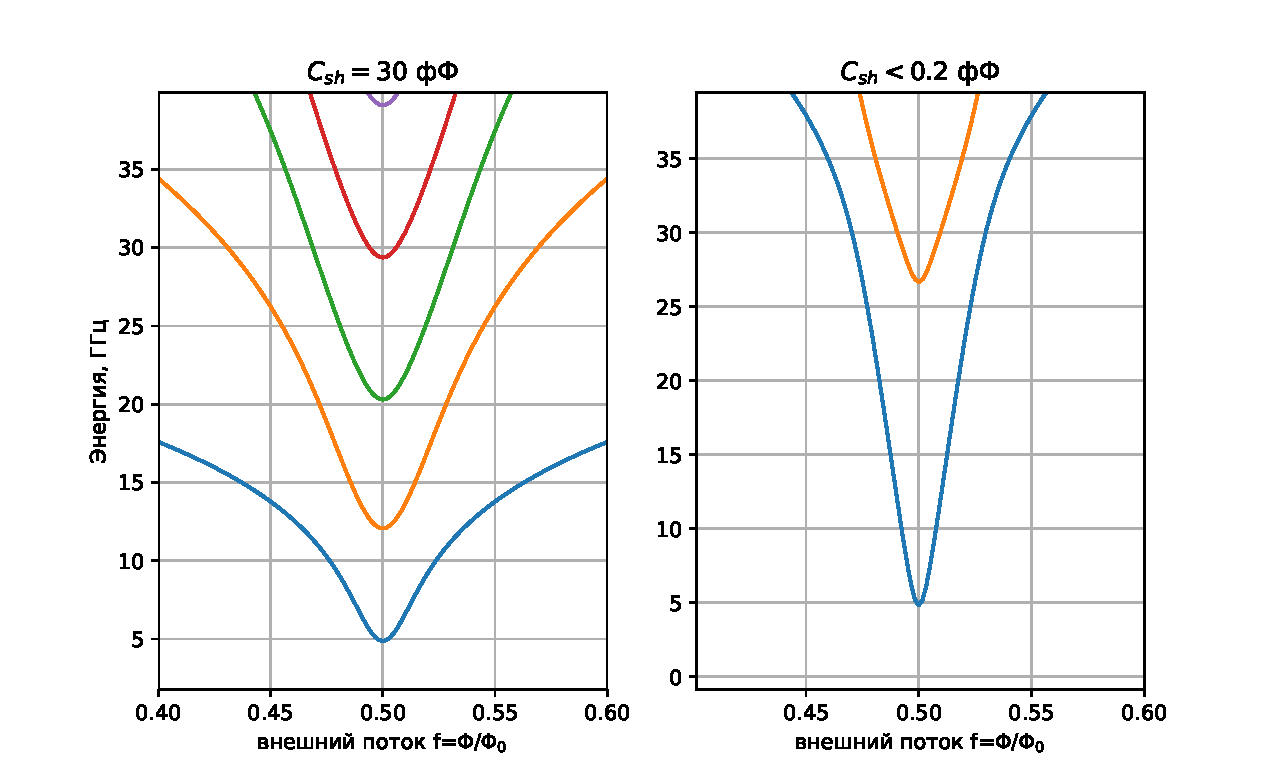
\includegraphics[width=1\textwidth]{images/3jj_spectra.pdf} \hfill
	\caption[Влияение шунтирующей емкости на спектры потоковых кубитов]{Рассчитанные спектры $E_n-E_0$ потоковых кубитов с тремя джозефсоновскими переходами с учетом влияния шунтирующей емкости $C_{sh}$ на $\alpha$-переходе. В обоих случаях $E_c = 25$~ГГц, $E_j=170$~ГГц. Левая панель: спектр для параметров $C_{sh} = 30$~фФ, $\alpha=0.5$. Правая панель: спектр для параметров $C_{sh} \approx 0.1$~фФ, $\alpha=0.69$. Как можно заметить, при равных параметрах переходов (что соответствует одинаковому процессу окисления) большая шунтирующая емкость сглаживает спектр и делает кубит не столь чувствительным к дефазировке по потоку, при этом ангармонизм еще достаточно велик (1-2 ГГц). В случае отсутствия шунта, приходится понижать частоту перехода 0-1 при помощи увеличения $\alpha$, однако, при смещении от оптимальной точки $f=0.5$ производная энергии по потоку значительно увеличивается, и такой кубит гораздо сильнее подвержен дефазировке. Кроме того, при отсутствии шунта верхние уровни имеют слишком высокую частоту и недоступны для использования.}
	\label{fig: 3jj_spectra}
\end{figure}
\subsection{Маршрутная карта для изготовления образцов}

Образцы кубитов изготавливались в условиях чистой комнаты класса ISO-5 (не более 1000 пылинок размером более 1 мкм в 1 м$^3$ воздуха). Маршрутная карта включает следующие процедуры:
\begin{enumerate}
	\item Отмывка подложки из высокоомного недопированного кремния 
	\begin{itemize}
	  \item дистилированная вода+ультразвук, 2 мин
	  \item IPA, 10 сек
	  \item NMP, 150 $^\circ$C, 5 мин
	  \item RCA-1+ультразвук, 80 $^\circ$C, 2 мин 
	\end{itemize}
	\item Нанесение копланарной линии
	\begin{itemize}
		\item нанесение резиста LOR-5B 3000 об/мин, 180$^\circ$C, 7 мин;
		\item нанесение резиста S1813 4000 об/мин, 115$^\circ$C 7 мин;
		\item фотолитография на литографе Heidelberg 8 мВ, 80%;
		\item проявка KOH 45 сек;
		\item напыление 100 нм пленки Al (Plassys), 0.2 нм/c; 
		\item лифт-офф NMP+ультразвук 100$^\circ$C, 5 мин;
	\end{itemize}
	\item Нанесение туннельных контактов
		\begin{itemize}
			\item нанесение резиста Copolymer/MMA 9\% 3000 об/мин, 150$^\circ$C, 5 мин;
			\item нанесение резиста ARP 6200.04 4500 об/мин, 150 $^\circ$C 5 мин;
			\item электронная литография на литографе Crestec CABL 9000 160 pA, 1 мкс/точка;
			\item проявка AR 600-546 1 мин, IPA 30 с, дистилированная вода 30 сек;
			\item напыление нижней пленки Al толщиной 25 нм под углом $+11^\circ$ (в установке Plassys), скорость напыления 0.2 нм/c.
			\item Промежуточное окисление при давлении 2 мБар в течение 5 мин; 
			\item напыление верхней пленки Al толщиной 45 нм под углом $-11^\circ$, 0.2 нм/c.
			\item лифт-офф NMP+ультразвук 100$^\circ$C, 5 мин;
		\end{itemize}
\end{enumerate}

Представленный процесс может быть изменен или дополнен. В ряде случаев перед напылением джозефсоновских контактов требуется удалить естественный слой оксида с алюминиевой пленки, для этого используется травление ионами Ar при помощи пушки. Типичные параметры: ускоряющее напряжение 400 В, ускоряющее напряжение 80В, ток эмиссии 20 мА, время 2 минуты.

Согласно даннной маршрутной карте были изготовлены образцы. При рассмотрении в оптическом микроскопе была проведена инспекция микронных структур на соответствие размерам, задаваемым в дизайне, см.~Рис. \ref{img: line_opt_control}.  При помощи СЭМ сделаны изображения изготовленных кубитов, см.~Рис. \ref{img: qubits_sem}. Можно наблюдать сформированные переходы, размеры которых близки к заложенным в дизайн значениям. Последний шаг проверки вновь сделанных образцов --- измерение нормального сопротиления тестового перехода или СКВИДа при помощи зондовой станции. Для переходов 200x800 получены значения в диапазоне $R_n=2.1-2.4$~кОм. Если предположить, что при падении температуры от комнатной до $T_c$ сопротивление уменьшается в 3 раза, то для джозефсоновской энергии имеем $E_J/h \approx 160$~ГГц. Однако, эта оценка является весьма неточной, поскольку точное значение нормального сопротивления джозефсоновского контакта вблизи сверхпроводящего перехода неизвестно, хотя в принципе может быть оценено из ВАХ отдельных переходов. 
\begin{figure}[htb]\center
	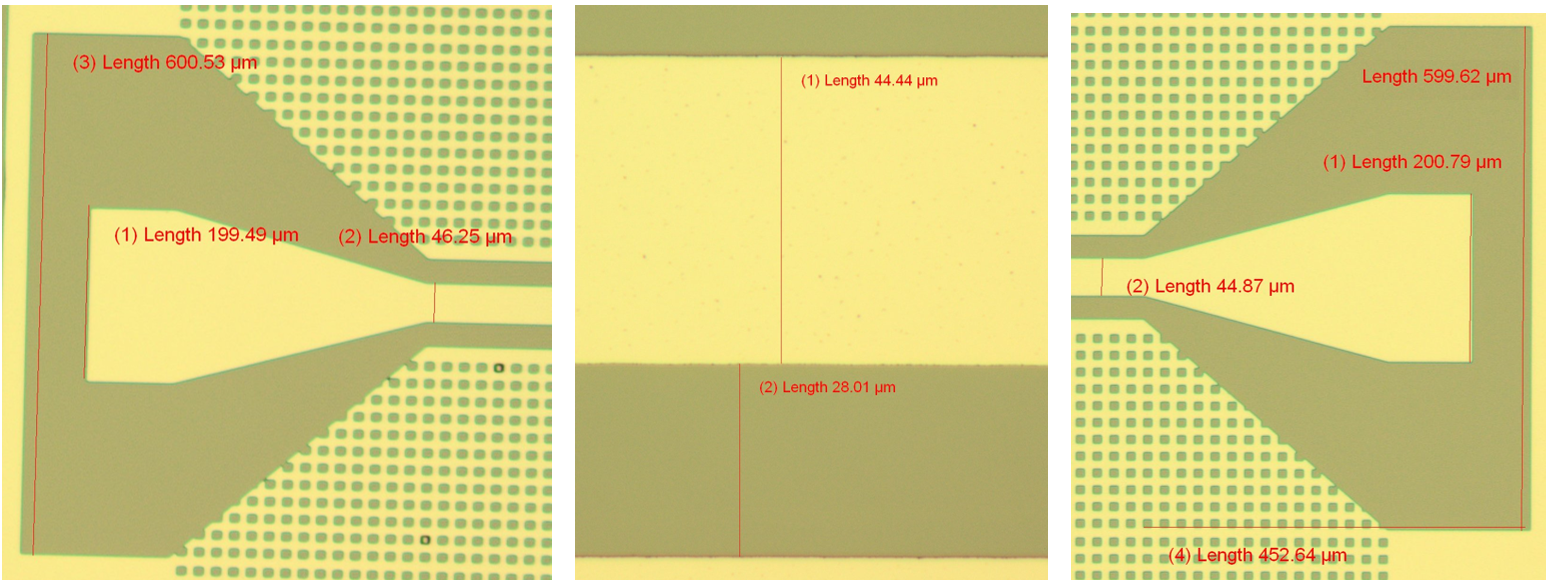
\includegraphics[width=1\textwidth]{line_opt_control.png} \hfill
	\caption[Контроль размеров микронных структур в оптическом микроскопе]{Контроль поперечных размеров копланарной линии  и контактных площадок при помощи оптического микроскопа. Размеры отклоняются от заложенных в дизайн значений не более чем на 1 мкм.}
	\label{img: line_opt_control}
\end{figure}

\begin{figure}[htb]\center
	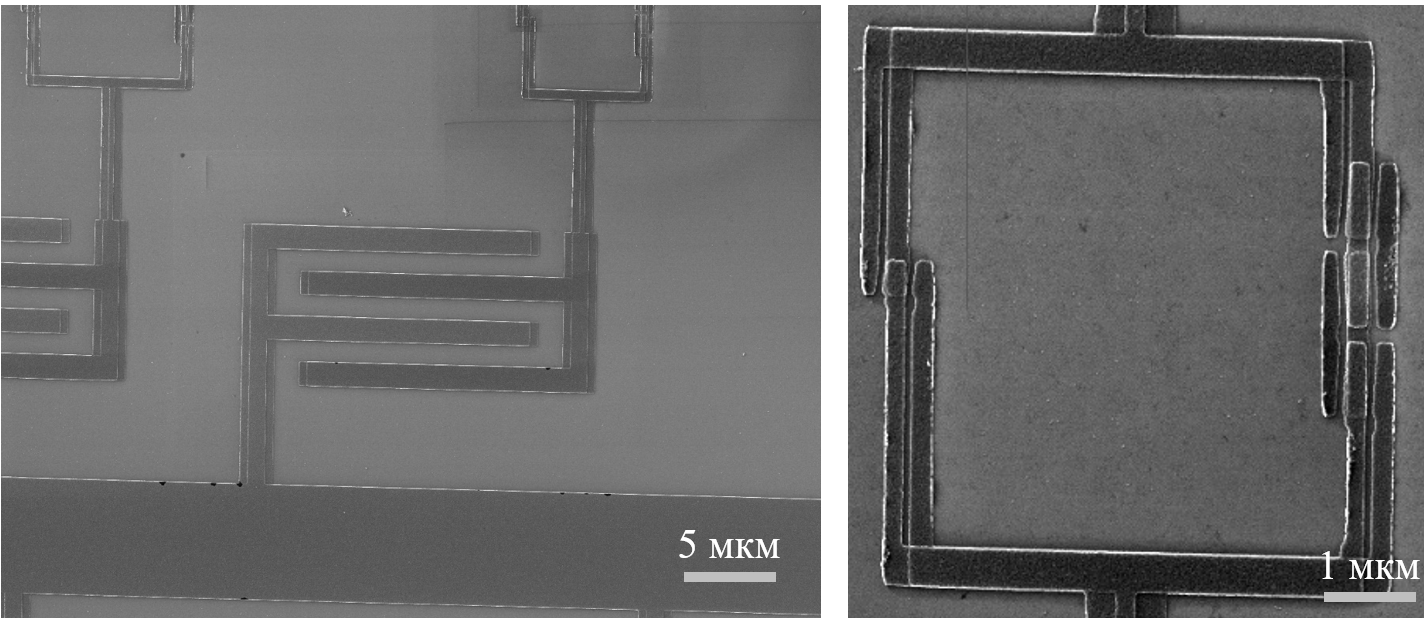
\includegraphics[width=1\textwidth]{qubits.png} \hfill
	\caption{Изображение связывающей емкости и кубита в сканирующем электронном микроскопе (СЭМ)}  
	\label{img: qubits_sem}
\end{figure}
Следующий шаг --- сборка измерительной схемы внутри криостата растворения и помещение в неё образца с кубитами для последующих измерений. 
\section{Схема подключения кубитов в линии}
После того, как чип с волноводом и кубитами изготовлен, необходимо  собрать измерительную схему, которая позволит осуществить экспериент по измерению нелинейного рассеяния на кубите. Для размещения чипов внутри криостата необходимо:
\begin{itemize}
	\item{разместить чип с кубитом внутри печатной платы, закрепленной на внутренней части высокочастотного низкотемпературного держателя;}
	\item{приклеить чип и осуществить ультразвуковую разварку контактных площадок высокочастотных линий на чипе к отрезкам копланарных линий печатной платы;}
	\item{собрать высоко- и низкочастотные входные и высокочастотные выходные линии по всей длине криостата, начиная от фланца с температурой 50 К и заканчивая ответной частью держателя на фланце с базовой температурой;}
	\item{вставить держатель с платой в его ответную часть, закрепляемую на нижней ступени рефрижератора;}
	\item{при помощи тестера определить сопротивления между центральными жилами сигнальных проводов и землей и между входной и выходной линиями держателя, подходящими к волноводу на чипе;}
	\item{соединить разьемы линий с разьемами держателя соотвественно;}
	\item{протестировать высокочастотное пропускание волновода, подключив входную и выходную линии к ВАЦ;}
	\item{в случае хорошего прохождения сигнала, загрузка считается успешной и можно приступить к охлаждению криостата.}
\end{itemize} 
Рассмотрим некоторые из этих манипуляций более подробно и опишем те свойства, которыми должна обладать измерительная схема для правильного функционирования образца. 
\subsection{Устройство держателя}

Первое и самое очевидное условие работы кубитов --- возможность охлаждения чипа до базовой температуры рефрижератора, которая равна 15-20 мК. Такую же температуру должна иметь и печатная плата, на которой размещается чип, и та часть держателя (бобышка), которая контактирует с печатной платой и кубитным чипом. Это налагает очевидные ограничения на те материалы, из которых может состоять держатель. Стальные сплавы имеют крайне низкую теплопроводность при температурах менее 1 К. Аналогичное можно сказать о любом сверхпроводнике, охлажденном ниже $T_c$ --- отсутствие свободных носителей тока ухудшает возможность переносить тепло. Поэтому все компоненты держателя должны быть изготовлены из меди (в крайнем случае из латуни). Наилучшую теплопроводность при температурах ниже 100 мК обеспечивает бескислородна медь, но использование обычной чистой меди (марка М1) практически не влияет на скорость охлаждения. 

Держатель состоит из нескольких обязательных частей --- печатная плата, бобышка, ответная часть, крепление к фланцу, магнитный и сверхпроводящий экраны и различные вспомогательные элементы. 

Печатная плата изготавливается из высокочастотного стека. Стек состоит из двух медных слоев толщиной порядка 100 мкм, разделенных диэлектриком с малыми потерями, например, Arlon AD-1000. Плата имеет сквозное отверстие для размещения чипа. К краям отверстия подходят копланарные линии, которые расходятся в радиальных направлениях и заканчиваются возле краев платы специальными расширениями, на которые впоследствии запаиваются высокочастотные разъемы. Плата предусматривает размещение от 4 до 12 SMP-разьемов типа <<папа>>, центральная жила которых запаивается на центральную дорожку копланарных высокочастотных линий. В эти разъемы затем вставляются коаксиальные провода с ответными SMP-разъемами, которые будут крепиться на ответной части держателя. 

Печатая плата плотно прикручивается к бобышке для обеспечения хорошего высокочастотного электрического контакта между нижней металлизацией печатной платы и объемом бобышки. Важный атрибут бобышки --- наличие прямоугольной полости в месте крепления чипа. Полость повторяет форму чипа и имеет глубину 5-7 мм. Она нужна для смещения резонансных объемных мод кремниевого чипа в область высоких частот, что особенно актуально для чипов больших размеров. Поскольку диэлектрическая проницаемость кремния достаточно велика: $\varepsilon=11.7$, то для чипа с продольным размером $a=10$ мм первая объемная мода имеет частоту $f_1 = c/2a\sqrt{\varepsilon}=4.33$~ГГц. Эта частота находится точно в середине рабочей области и потому может легко возбуждаться, если попадает в резонанс с сигналом в копланарной линии на поверхности чипа. Однако, если добавить полость под чипом и рассмотреть вновь получившийся объемный резонатор, то эффективная $\varepsilon$ упадет в несколько раз, и объемные моды перестанут оказывать прямое влияние на распространение сигнала по копланарным линиям на чипе. 

Бобышка с печатной платой вставляется в ответную часть держателя. Ответная часть представляет из себя цилиндрическую полость без дна (дном служит бобышка). В верхнем торце ответной части располагаются отверстия, которые располагаются точно над SMP-разъемами печатной платы. Через эти отверстия проходят провода, подключающиеся к SMP-разъемам. В середине ответной части имеется ушко, за которое она подвешивается к штанге длиной около 30 см. Штанга, в свою очередь, прикрепляется к крепежному фланцу. Крепежный фланец имеет сквозные отверстия для SMA-переходников и крепления для магнитного и сверхпроводящего экранов. SMA-переходники накручиваются на сквозные отверстия. На внутренние разъемы переходников накручиваются провода, идущие к печатной плате, а на внешние разъемы переходников приходят (с внешних разъемов уходят) входные (выходные) коаксиальные линии. Также в фланце имеется отверстие для пары проводов, запитывающих сверхпроводящий соленоид. Соленоид наматывается на боковую поверхность ответной части держателя, а контакты выводятся через отверстие и подключаются к линиям постоянного тока, выходящим на фланец с базовой температурой.

Поскольку кубиты чувствительны к внешнему магнитному полю, чипы необходимо экранировать от магнитного поля Земли и от другого паразитного магнитного поля шума, которое создают электрические приборы. Для этого на фланец надевается цилиндрический сверхпроводящий экран. Этот экран будет захватывать магнитное поле благодаря эффекту Мейснера. Имеется возможность дополнительно уменьшить поле, которое будет вытесняться сверхпроводящим экраном. Для этого поверх сверхпроводящего экрана надевается еще один экран из криогенного пермаллоя (Cryoperm) - мягкого магнитного металла с очень большим значением магнитной восприимчивости $\mu \approx 10^5$. Силовые линии магнитного поля концентрируются внутри криоперма, а магнитное поле внутри экрана будет ослаблено (в идеале в $\mu$ раз, на практике далеко не так эффективно из-за того, что экран не имеет крышки.). Описанное решение является относительно стандартным и с теми или иными модификациями (например, использование второго криопермового экрана вместо сверхпроводящего) используется во многих исследовательских группах, работающих со сверхпроводящими кубитами. Непосредственная проверка эффективности ослабления внешнего магнитного поля не проводилась, но в ходе экспериментов, описываемых в данной работе, не возникало явных указаний на критически значимые магнитные шумы. 

Мы завершили общее описание держателя. Теперь необходимо изложить требования, которые предъявлются к схеме измерения кубитов.

\subsection{Требования к измерительной схеме}
Схема измерения кубитов в линии включает в себя низкотемпературную часть внутри криостата растворения и управляющую электронику при комнатной температуре, которая подключается к криостату и управляется при помощи компьютера. Низкотемпературная часть схемы изображена на Рис. \ref{fig: schemes} для случая параллельной связи (неразрывная линия с кубитом) и для случая прямой связи (кубит связан с двумя полубесконечными линиями). 
\begin{figure}[htb]\centering
	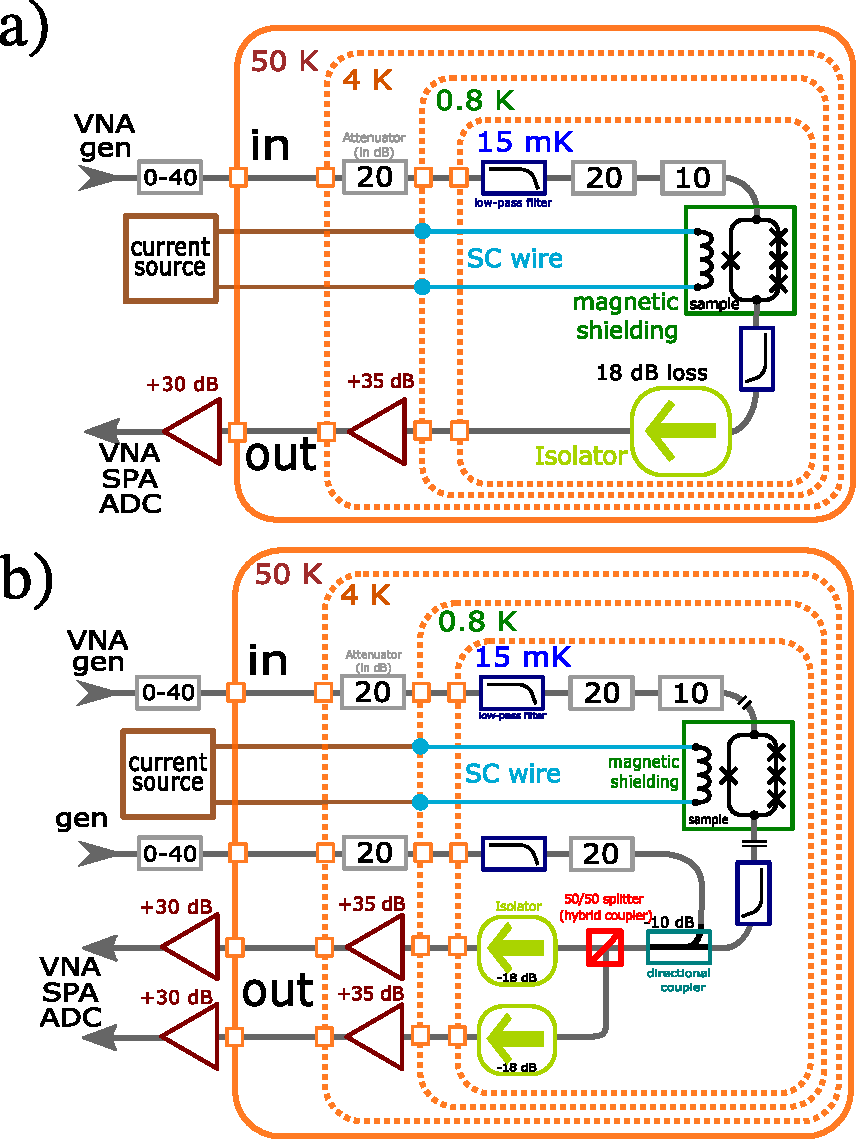
\includegraphics[width=0.8\textwidth]{images/meas_schemes_2.pdf} \hfill
	\caption{Низкотемпературная часть измерительных схем. а) --- схема для кубита в линии (параллельная связь), б) --- схема для кубита, связанного с двумя полупространствами (прямая связь) }
	\label{fig: schemes}
\end{figure}

Сначала обсудим общие свойства изображенных схем. На Рис. \ref{fig: schemes} оранжевыми пунктирными линиями выделены различные ступени криостата растворения. Держатель с чипом располагается внутри магнитного экрана при базовой температуре (примерно 15 мК). К нему подходят входные высокочастотные коаксиальные линии внутри криостата (на Рис. \ref{fig: schemes} обозначены серым цветом). На каждой ступени в линии включаются аттенюаторы с различным номиналом (от 0 до 20 дБ ослабления) для термализации теплового шума, который распространяется далее по линии. Выходной сигнал, как правило, имеет очень малую мощность, и необходимо обеспечить минимальные потери до первого усиления. По этой причине выходные коаксиальные линии  делаются сверпроводящими от чипа до низкотемпературных усилителей (коричневые треугольники), располагающихся на 4К-фланце (фланце с температурой около 4 кельвин). На эти линии нельзя поставить аттенюаторы для ослабления теплового шума. Поэтому защитить чип от тепловой радиации можно лишь при помощи магнитных изоляторов (изображены на схемах зелеными стрелками) --- диодов для высокочастотного сигнала, которые почти не ослабляют СВЧ-сигнал в прямом направлении, но дают примерно 18-20 дБ в обратном направлении.  Низкочастотные линии (на Рис. \ref{fig: schemes} коричневые/голубые) представляют из себя витые пары, которые подключаются к соленоиду, а также подводят питание для радиочастотных переключателей, которые располагаются на базовой ступени криостата и дают возможность подключать к одной выходной линии несколько входных (на схемах переключатели не показаны, поскольку в описываемых далее экспериментах они не использовались).

Как уже упоминалось ранее, кубит должен находиться в тепловом равновесии при базовой температуре криостата 15 мК. Ранее мы пояснили, что хороший тепловой контакт чипа с держателем является одним из условий, способствущих хорошему охлаждению кубита. Однако влияние на состяоние кубита имеет не столько фононная температура чипа (которая действительно близка к базовой), сколько температура электронной подсистемы. Условие эффективной термализации электронной системы сверхпроводящей цепи на чипе --- эффективное ослабление теплового шума, который испускают электронные приборы на комнатной температуре. Правильная расстановка аттенюаторов без каких-либо дополнительных действий снижает электронную температуру до 50 мК, что можно подтвердить из независимого определения температуры при помощи, например, термометра на основе эффекта кулоновской блокады \cite{Meschke2004}. Для дальнейшего понижения температуры требуется установка ИК-фильтров \cite{Longobardi2013}, предотвращающих распространение фотонов частотами от 20 до нескольких сотен ГГц в коаксиальных линиях. Для описанных в работе измерений ИК-фильтры не применялись. Рассмотрим более подробно, как аттенюаторы ослабляют тепловой шум, проникающий в криостат растворения.

\subsection{Ослабление теплового шума}
Любой активный электронный прибор (например, СВЧ-генератор), располагающийся на комнатной температуре и имеющий выходное сопротивление $Z_0$, будет выдавать на выход некоторый шум. В целом, электронный шум включает в себя дробовой шум, который зависит от протекающего тока, низкочастотный шум $1/f$, характерный для всех типов полупроводниковых электронных приборов, а также тепловой шум. Спектральные плотности дробового шума и фликер-шума $1/f$ при комнатной температуре пренебрежимы по сравнению со спектральной плотностью теплового шума Джонсона-Найквиста, которую можно записать как:
\begin{equation}
S_V(T, \omega) =\frac{2\hbar \omega Z_0}{1-\exp\left(-\hbar\omega/k_bT\right)}
\label{eq: J-N}
\end{equation}

При высоких температурах $\hbar \omega \ll k_b T $. Тогда из \eqref{eq: J-N} получаем классическое выражение $S_V(\omega) = 2k_bTZ_0$, а значит, на начальных стадиях при $T \gg $ 1~К тепловой шум нужно ослаблять пропорционально температуре ступени. Однако, при более низких температурах это простое правило уже не работает, и ослаблять тепловой шум нужно значительно сильнее. Чтоб пояснить это, отметим, что спектральная плотность шума напряжения \eqref{eq: J-N} может быть рассчитана как для положительных, так и для отрицательных частот. Разница особенно заметна при нулевой температуре: $S_V(0,\ {\omega\! <\! 0})=0$, тогда как $S_V(0,\ {\omega\! >\! 0})=2Z_0 \hbar\omega$. Физический смысл этого различия можно пояснить, вычислив скорости возбуждения и релаксации двухуровневой квантовой системы под действием шума \cite{schoelkopf2003qubits}. Если кубит взаимодействует с внешним напряжением в дипольном приближении $H_{int} = A V(t) \sigma_x$, то из теории возмущений можно получить:
\begin{equation}
\Gamma_\downarrow = \frac{A^2}{\hbar^2}S_V(+\omega_q), \quad \Gamma_\uparrow = \frac{A^2}{\hbar^2}S_V(-\omega_q).
\end{equation}
\begin{figure}[h]\centering
	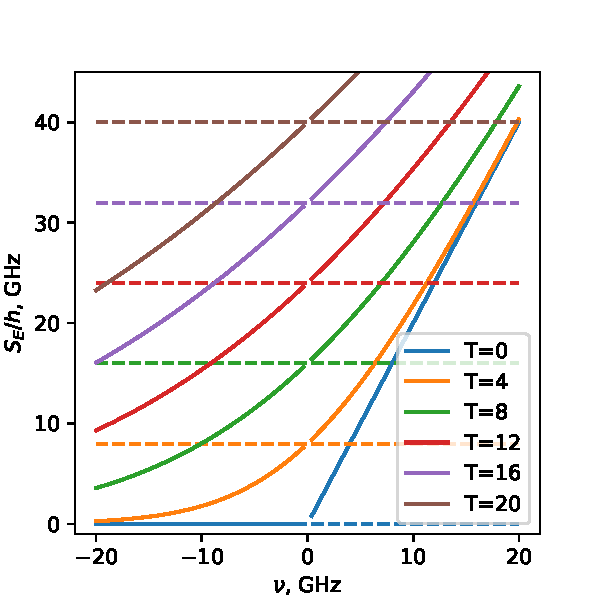
\includegraphics[width=0.7\textwidth]{QN_spectrum.pdf} \hfill
	\caption[Спектральная плотность флуктуаций напряжения]{Спектральная плотность флуктуаций напряжения в зависимости от нормированной температуры $T/k_b h$ и частоты $\nu=\omega/2\pi$ (в ГГц) согласно выражению \eqref{eq: J-N}. Пунктирная линия отмечает классическое выражение для спектральной плотности $S_V = 2 k_b T$. }
	\label{img: S_V}
\end{figure}
Таким образом, шум на отрицательных частотах может поглощаться и вызывать возбуждение системы. Наоборот, спонтанную релаксацию возбужденного кубита (или резонатора в квантовом режиме) вызывает шум на положительных частотах. Поэтому для эффективной термализации кубита частотой $\omega_q$, расположенного при базовой температуре $T_b$ нужно ослабить шум верхних ступеней до уровня $S_V(T_b, -\omega_q)$. 

Точный расчет остаточного числа фотонов, достигающего базового фланца при различных номинальных значениях аттенюаторов, показывает \cite{krinner2019engineering}, что наиболее оптимальная конфигурация с точки зрения ослабления остаточного шума предусматривает расположение по 20 дБ ослабления на 4К-ступени, на промежуточном фланце температурой около 100 мК между фланцем Still температурой 0.8 К и базовым фланцем температурой 10-15 мК), и на базовом фланце --- всего 60 дБ ослабления. Однако, чтоб иметь возможность сильно увеличивать амплитуду драйва, в экспериментах использовалось 40-50 дБ ослабления за счет уменьшения номинала аттенюатора на ступени с температурой 100 мК до 10 дБ, либо полного его снятия.

\subsection{Усиление рассеянного сигнала}
\label{sec: amplif}
Как выяснено в предыдущем подразделе, после прохождения входной линии тепловой шум  ослабляется для предотвращения нежелательной зачеселенности кубита. Аналогичным образом ослабляется и управляющий кубитом когерентный сигнал. Как ясно из представленных в разделе \ref{sec: microwave qo} расчетов, характер действия поля на кубит, и соотвественно, характер рассеяния когерентного сигнала определяются амплитудой Раби $\Omega$ и отстройкой от кубита $\delta\omega$. На выходе из волновода к исходному сигналу добавляется рассеянное на кубите поле, определяемое выражением \eqref{eq: sc_field}. Эквивалентную мощность этого сигнала можно оценить как:
\begin{equation}
P_{sc} = \frac{|V_{sc}|^2}{2Z_0} \approx \frac{(\hbar \Gamma_1/2e)^2}{2Z_0} \approx -155 \text{ дБм}.
\label{eq: P_sc}
\end{equation}
Оценка сделана в приближении $\mu\!\approx\!2e$ и для $\Gamma_1\!=\!2\text{ МГц.}$. Отсюда можно сделать два вывода. Во-первых, перед измерением столь малый сигнал необходимо значительно усилить, поскольку типичные ВАЦ и СА могут обнаруживать сигналы мощностью около -100 дБм. Во-вторых, очевидно, что необходимо использовать малошумящие низкотемпературные усилители, поскольку эквивалентная температура, соотвествующая мощности \eqref{eq: P_sc} в полосе $\Gamma_1$, примерно равна:
\begin{equation}
T_{eq} = \frac{P_{sc}}{4k_b\Gamma_1} = 2.8 \text{ мК}. 
\end{equation}
В экспериментальной установке в качестве первого каскада усиления используются доступные в коммерческих целях усилители фирмы Low Noise Factory с эквивалентной шумовой температурой 2-4 К, так что даже в случае их использования отношение <<сигнал-шум>> по порядку величины не превышает 1/100. Эти усилители располагаются на ступени с температурой 4 К. Дальнейшее усиление осуществляется при помощи комнатных высокочастотных усилителей Mini Circuits ZVA-183+ или их аналогов. Общее усиление составляет примерно 80-100 дБ при использовании узкополосных приборов (например, при измерении стационарного поля) и 120-140 дБ при использовании высокочастотных ЦАП. Это вызвано тем, что битность высокочастотных ЦАП ограничена, и для качественной оцифровки требуется сигнал более высокой амплитуды.

\section{Спектроскопия кубитов}

Как выяснено в разделе \ref{subsec: flux_q}, частота потокового кубита перестраивается магнитным потоком, пронизывающим контур кубита. Трансмон со СКВИДом вместо джозефсоновского перехода также перестраивается магнитным полем. По этой причине первичным измерением потокового (как и практически любого другого) кубита в волноводе является однотоновая спектроскопия. Входная и выходная линия подключаются к ВАЦ, после чего измеряется коэффициент пропускания $S_{21}$ в зависимости от тока в катушке или в потоковой линии. Это позволяет найти частоту кубита при различных потоках, в частности, найти оптимальные по потоку точки, если это необходимо для дальнейших измерений. 

На Рис.~\ref{img: circlefit} изображена частотная характеристика кубита в линии при базовой температуре, полученная при помощи ВАЦ в режиме $\Omega \ll \Gamma_1$. В случае очень слабой накачки поведение кубита в линии ничем не отличается от резонатора, включенного параллельно линии по схеме типа <<notch-порт>>. Детальная модель частотной характеристики для таких резонаторов была построена в работах \cite{gao2008physics,Khalil}. В рамках этой модели показано, что пропускание через такой резонатор представляет собой ассимметричный лоренцевский пик, описываемый выражением:
\begin{equation}
S_{21}^\text{notch}(f) = \underbrace{\vphantom{\frac{Q_l e^{i\phi}}{1+2iQ_l\left(f/f_r -1  \right)}}  a e^{i\alpha} e^{-2\pi i f \tau}}_{\text{окружение}} \underbrace{\left[ 1 - \frac{\left(Q_l/ |Q_c|\right) ~ e^{i\phi}}{1+2iQ_l\left(f/f_r -1  \right)}  \right]}_{\text{идеальный резонатор}}\,.
\label{eq:S21model}
\end{equation}
Опишем некоторые свойства модели:
\begin{itemize}
	\item {модель учитывает частотно-зависимый набег фазы $-2\pi i f \tau$, который возникает из-за задержки распространения сигнала через тракт $\tau$;} 
	\item {связь к линии характеризуется при помощи добротности связи $Q_c$ (комплексная величина);}
	\item {модель учитывает дополнительный фазовый сдвиг $i\phi$ комплексного сигнала, соотвествующего пику резонатора на частоте резонанса $f_r$. Этот сдвиг возникает из-за индуктивного импеданса бондирующих проводов, а также из-за несогласований на переходниках по ходу коаксиальных линий;}
    \item {внутренние потери в резонаторе описываются внутренней добротностью $Q_i$, которая может быть выражена через полную (нагруженную) добротность резонатора в линии $Q_l$:
    	\begin{equation}
    	Q_i^{-1} = Q_l^{-1} - \text{Re}\left\{ Q_c^{-1} \right\}.
    	\end{equation}}
\end{itemize}
\begin{figure}[h]\centering
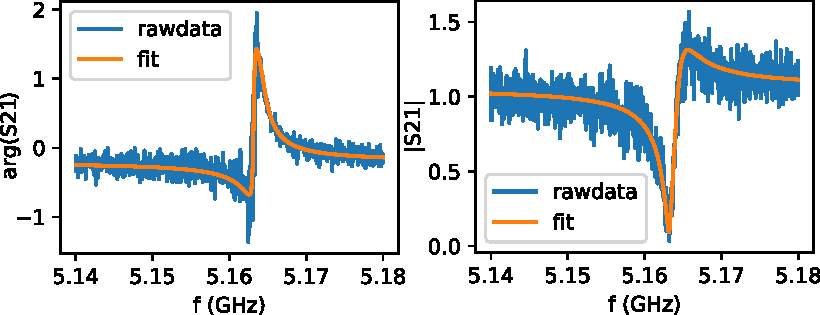
\includegraphics[width=1\textwidth]{qubit_circlefi_2_edit.pdf} \hfill
\caption[Пропускание волновода с кубитом]{Частотная характеристика коэффициента прохождения $S_{21}(f)$ высокочастотного маломощного сигнала через волновод с кубитом. Измеренный сигнал нормирован на фоновое пропускание, измеренное при большой мощности, либо же при значительной отстройке кубита. Данные подогнаны при помощи модели резонатора в линии (см. основной текст), параметры фита отображены в Табл.~\ref{Tab1}.}
\label{img: circlefit}
\end{figure} 
\begin{table} [htbp]
	\centering
	\changecaptionwidth\captionwidth{15cm}
	\caption{Параметры модели пропускания резонатора}\label{Tab1}%
	\begin{tabular}{| p{2.2cm} | p{3cm} | p{3cm}l |}
		\hline
		\hline
		Параметр   & \centering Значение & \centering Ошибка & \\
		\hline
		$Q_i$ &\centering  20275  &\centering 2225 & \\
		$Q_c$ &\centering  2448  &\centering  49 &\\
		$f_r$, Гц &\centering  5.164$\cdot10^9$  &\centering 4.43$\cdot10^4$ &\\
		$\phi$, рад &\centering  -0.681  &\centering  0.025 & \\
		\hline
		\hline
	\end{tabular}
\end{table}
Измеренный коэффициент $S_{21}$ был подогнан при помощи репозитория \verb|circlefit|, разработанного в \cite{Probst_circlefit}. Результаты измерения пропускания кубита с наложенной линией подгонки изображены на Рис. \ref{img: circlefit}. Можно заметить, что модель хорошо описывает экспериментальные данные. Результат подгонки дает значения $ Q_i, Q_c, f_r \text{ (для кубита уместнее обозначение }f_q)$ и других параметров, которые приведены в Табл.~\ref{Tab1}.

Добротность связи кубита с линией можно связать со скоростью излучательной релаксации:  $\Gamma^r_1/2\pi= f_q/Q_c = 2.1$~МГц на основе данных из Табл.~\ref{Tab1}. Внутренняя добротность можно списать на всевозможные причины, по которым когерентный сигнал не достигает ВАЦ после рассеяния на кубите. Это безызлучательная релаксация, в которую можно включить потери в кубите и релаксацию в какие-либо паразитные моды, а также чистая дефазировка: $\left(\Gamma_1^{nr} + 2\Gamma_\varphi \right)\!/2\pi = f_q/Q_i = 255\text{ кГц}$, опять же на основе Табл.~\ref{Tab1}.

Однотоновая спектроскопия представляет собой измерение, при котором линия пропускания кубита, показанная на Рис.~\ref{img: circlefit}, измеряется при различных значениях магнитного потока в катушке или в токовой линии, при этом частоа кубита перестраивается. В результате получаются спектры потоковых 
кубитов, пример которых приведен на Рис.~\label{img: singletone}. 

\begin{figure}[h]\centering
	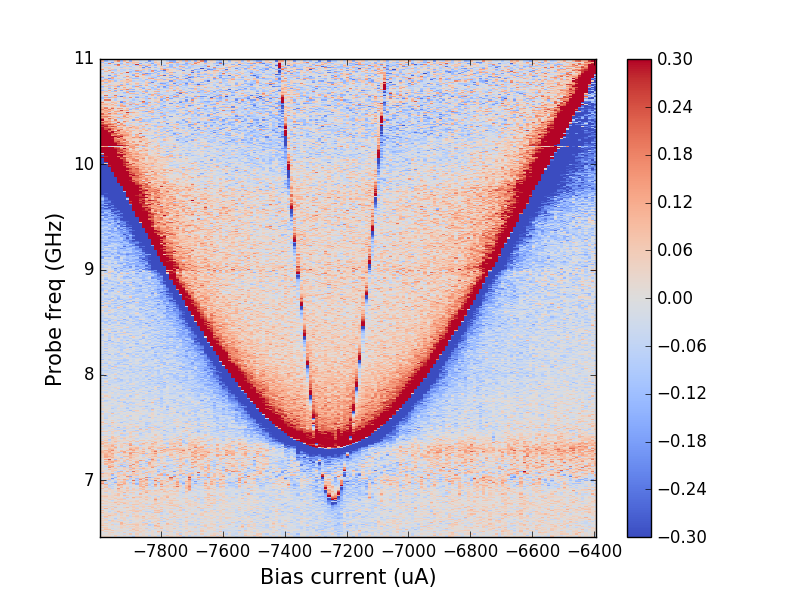
\includegraphics[width=0.9\textwidth]{FluxQ_spectra4_both.png} \hfill
	\caption[Измеренные спектры потоковых кубитов]{Однотоновая спектроскопия потоковых кубитов: $\arg\left(S_{21}(f) \right)$ в зависимости от тока через катушку держателя. Можно различить спектры двух кубитов с различным значением $\Gamma_1$, соотвествующие различным связывающим емкостям на Рис.~\ref{img: 4jj_side}} 
	\label{img: singletone}
\end{figure} 
 
У типичного потокового кубита отсутствует большая емкость, и спектр вблизи минимума энергии представляет собой гиперболу, однако, для реального кубита емкость меняет собственные состояния: они становятся не просто суперпозицией двух туннельно связанных потоковых состояний, но оказываются более сложными по своей сути. Поэтому при необходимости точной подгонки спектра используется численная диагонализация гамильтониана в каждой точке по магнитному потоку, как было описано в разделе \ref{subsec: flux_q}. Спектральная линия повторяется с периодом $\Phi_0$, и при необходимости из измерения периода по току можно оценить эффективную площадь контура потокового кубита. 

Интересно отметить, что на некоторых спектрах наблюдаются антипересечения линии кубита с некоторой резонансной системой, которые обусловлены когерентным взаимодействием с дефекными двухуровневыми системами, см. Рис.~\ref{img: anticross}. Как правило, эти системы расположены внутри слоя AlOx джозефсоновского контакта, и устранить их практически невозможно. Наличие дефектов в джозефсоновском переходе --- еще одна причина ограничения размеров джозефсоновского контакта: при большой площади переходов плотность дефектов становится достаточно значительной, что портит кубит и делает работу с ним невозможной. Именно поэтому необходимо изготавливать джозефсоновские переходы при помощи электронно-лучевой литографии, дающей разрешение примерно до 50 нм. 

Полученные в ходе однотоновой спектроскопии данные иллюстрируют стационарное рассеяние маломощного когеретного сигнала на кубите. Чтобы увидеть эффект насыщения, необходимо зафиксировать магнитное поле и измерить линию кубита в зависимости от амплитуды поля $\Omega$. 

Таким образом, кубит обнаруживает себя в спектроскопических измерениях, проводимых при помощи ВАЦ. 

\begin{figure}[h]\centering
	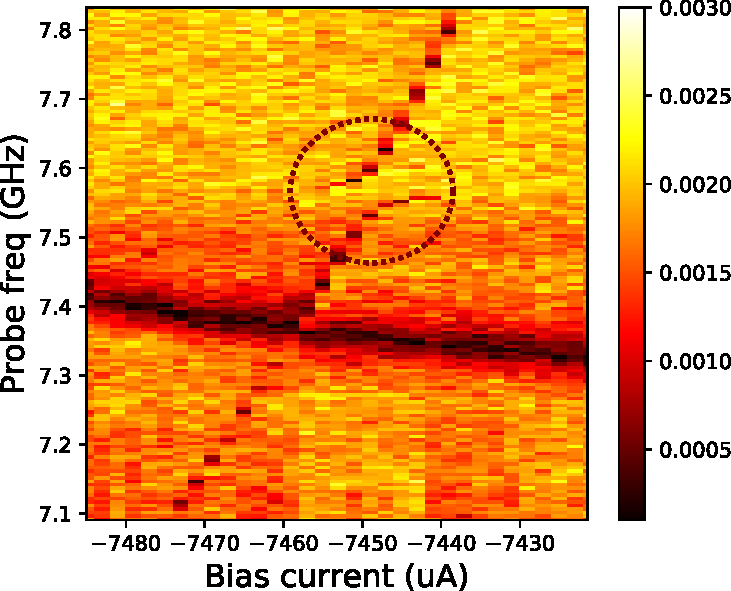
\includegraphics[width=0.7\textwidth]{STS_Anticross_ed.pdf} \hfill
	\caption[Взаимодействие кубита с резонансной двухуровневой системой]{Пример антикроссинга спектра кубита (узкая линия) с паразитной двухуровневой системой. Антикроссинг выделен кружком.} 
	\label{img: anticross}
\end{figure}

\section{Временная динамика состояния кубита}
рассказ об импульсных схемах и несколько картинок Раби (мб с фитом)

\section{Кубит в качестве нелинейной среды}
После того, как промерена однотоновая спектроскопия кубита и измерена его эволюция под действием внешнего поля, необходимо убедиться в нелинейном поведении кубита в линии. В традиционной оптике используется для этого вводится понятие \textit{нелинейной среды}, в которой нарушается пропорциональность электрического поля и поляризации. При распространении света в некотором веществе быстро осциллирующее электрическое поле волны $\tilde{E}(t)$ поляризует атомы или молекулы этого вещества. Поляризация среды может быть представлена в виде:
\begin{equation}
\tilde{P}(t) = \epsilon_0\left(\chi^{(1)}\tilde{E}(t) + \chi^{(2)}\tilde{E}^2(t) + \chi^{(3)}\tilde{E}^3(t) + \ldots\right)
\label{eq: nonlin_susc}
\end{equation}
Коэффициенты $\chi^{(2)}$ и $\chi^{(3)}$ называются нелинейной восприимчивостью. Разложение \eqref{eq: nonlin_susc} применимо в том случае, когда излучение нерезонансно, то есть его частота не совпадает с частотами атомных или молекулярных переходов. В случае одиночного искусственного атома мы имеем дело с насыщаемым рассеивателем --- двухуровневой системой, которая поляризуется под воздействием внешней волны. Значение поляризации атома можно получить как среднее значение дипольного момента, взятое по стационарному состоянию:
\begin{equation}
\tilde{P}(t) = \tr(\hat{\mu}\hat{\rho}_{st}) = \mu_{01}\rho_{10} + \mu_{10}\rho_{01}.
\end{equation}

Пользуясь \eqref{eq: stat_sol} и определяя восприимчивость из соотношения $\tilde{P} = \chi\tilde{E}$, получаем:
\begin{equation}
\chi = \frac{|\mu|^2}{\epsilon_0\hbar\Gamma_2}\frac{i-\delta\omega/\Gamma_2}{1+(\delta\omega/\Gamma_2)^2 + \Omega^2/\Gamma_1\Gamma_2},
\end{equation}
см. также \cite{boyd2003nonlinear}. Как мы отмечали ранее, выражение $\Omega^2/\Gamma_1\Gamma_2$ характеризует степень насыщенности двухуровневой системы и может быть обозначено как ${E^2}/{E^2_s}$, где $E_s$ --- напряженность насыщения: 
\begin{equation}
E_s = \frac{\hbar^2\Gamma_1\Gamma_2}{4|\mu|^2},
\label{eq: E_s}
\end{equation}
В общем случае, выражение $\Omega^2/\Gamma_1\Gamma_2$ не является малым и поэтому использовать разложение \eqref{eq: nonlin_susc} по степеням $\Omega \sim E$ в явном виде нельзя. Тем не менее, мы можем написать первые члены этого разложения:  
\begin{equation}
\chi\approx\frac{|\mu|^2}{\epsilon_0\hbar\Gamma_2}\frac{i-\delta\omega/\Gamma_2}{1+(\delta\omega/\Gamma_2)^2}\left[1-\frac{1}{1+(\delta\omega/\Gamma_2)^2}\frac{E^2}{E^2_s}\right].
\label{eq: chi}
\end{equation}
Можно отметить, что слагаемое, пропорциональное $E^2$, характерно для нелинейной восприимчивости $\chi^{(3)}$, тогда как $\chi^{(2)}=0$ для кубита. Это согласуется с общим свойством нелинейных центросимметричных сред, в которых возникает нелинейность третьего и более высоких порядков, но отсутствует нелинейность второго порядка. 
Концептуально близкое к задаче рассеяния волны на кубите явление из нелинейной оптики --- зависящий от мощности показатель преломления среды, или т.н. оптический эффект Керра. Известно, что при эффекте Керра возникающая нелинейная поляризация среды может быть записана в виде:
\begin{equation}
\tilde{P}^{N\!L} = \chi \tilde{E} = \left(\chi^{(1)} + 3\chi^{(3)}\tilde{E}^2\right)\tilde{E}.
\label{eq: P_NL}
\end{equation}
Сопоставляя \eqref{eq: P_NL} и \eqref{eq: chi}, получаем выражение для $\chi^{(3)}$:
\begin{equation}
\chi^{(3)} = -\frac{|\mu|^2}{3\epsilon_0\hbar\Gamma_2}\left[\frac{\delta\omega/\Gamma_2-i}{1+(\delta\omega^2/\Gamma^2_2)^2}\frac{1}{E^2_s}\right] = \frac{4}{3}\frac{|\mu|^4}{\epsilon_0\hbar^3\Gamma_1\Gamma_2^2}\frac{i-\delta\omega/\Gamma_2}{(1+\delta\omega^2/\Gamma_2^2)^2}.
\label{eq: chi_3}
\end{equation}
Полученный результат можно использовать для сравнения величины нелинейности, возникающей на кубите, с типичными значениями $\chi_{(3)}$ в задачах традиционной видимой оптики. Для наблюдения резонансной флуоресценции в видимом диапазоне свет может рассеивается, к примеру, на разреженном газе из атомов натрия. Таблица \ref{Tab2} иллюстрирует основные экспериментальные параметры, определяющие нелинейность, и конечные значения нелинейной восприимчивости. 
\begin{table} [htbp]
	\centering
	\changecaptionwidth\captionwidth{15cm}
	\caption{Экспериментальные характеристики нелинейных квантовооптических систем в открытом пространстве}\label{Tab2}%
	\begin{tabular}{| p{2.4cm} | p{3.2cm} | p{3.2cm}l |}
		\hline
		\hline
		Параметр   & \centering Кубит в линии & \centering Пары натрия \cite{boyd2003nonlinear} & \\
		\hline
		$N$ &\centering  $1$  &\centering $10^{14}$ & \\
		$\mu$, Кл$\cdot$м &\centering  $\sim 10^{-24}$   &\centering  $\sim10^{-29}$ &\\
		$\delta\omega$, Гц &\centering  $\sim 0$  &\centering $\sim10^{10}$ &\\
		$\Gamma_1$, Гц &\centering  $\sim10^6$  &\centering $\sim10^8$ & \\
		$\Gamma_2$ &\centering  $\Gamma_1/2$  &\centering $\Gamma_1/2$ & \\
		$\chi^{(3)}$, \text{м}$^2$/\text{В}$^2$ &\centering $\sim i\cdot 10^{-15}$   &\centering  $\sim 10^{-16}$ & \\
		\hline
		\hline
	\end{tabular}
\end{table}

Отметим ряд принципиальных различий между рассеянием микроволн на одиночном кубите и рассеянии видимого света на облаке атомов. Во-первых, имеется принципиальная возможность изучать рассеяние при нулевой отстройке $\delta\omega\!=\!0$. В случае облака атомов, на резонансной частоте перехода происходит сильное многократное поглощение (и переизлучение) света во всех направлениях, и задетектировать их чрезвычайно сложно. В свою очередь, одиночный кубит излучает поле в копланарный волновод, это поле усиливается криогенным усилителем и измеряется при помощи АЦП. С учетом небольших потерь в коаксиальных проводах и аттенюаторов на 0 дБ, через которые сигнал с кубита проходит перед попаданием на усилитель, схема позволяет измерить до 99\% сигнала, рассеянного кубитом, что проявляется в экспериментах по генерации одиночных фотонов \cite{ZhouHighEfficiency}.

Суммируя вышеизложенное, нелинейность на одном искусственном атоме по порядку величины практически сравнивается с нелинейностью макроскопического количества атомов в нелинейной среде. Это дает возможность изучать необычные квантовые эффекты в рамках нелинейной оптики, о которых пойдет речь в следующих главах данной диссертационной работы. 



           % Глава 2
\chapter{Двухчастотное волновое смешение на кубите: случай непрерывных волн}
\label{ch: cwm}
Основные экспериментальные результаты работы заключается в изучении волнового смешения на двухуровневой системе, играющей роль искусственного атома в открытом пространстве. Прежде чем перейти конкретно к выполненному в рамках работы эксперименту --- рассеянию двух почти резонансных микроволн на кубите --- рассмотрим основные принципы волнового смешения в том классическом виде, в котором оно описывается в нелинейной оптике сплошных сред для случая смешивания на ансамблях двухуровневых систем.
\section{Оптическое волновое смешение: случай распределенной среды и слабого пробного сигнала}
Рассматриваемый в имеющейся литературе по нелинейной оптике случай волнового смешения является одним из примеров большого класса нелинейных параметрических процессов --- процессов генерации новых частотных компонент или изменения исходных компонент при распространении света в нелинейной среде. Такие процессы удобно описывать при помощи волнового уравнения, учитывающего нелинейную поляризацию среды $\mathbf{P}^{N\!L}$. В классическом учебнике \cite{boyd2003nonlinear} показано, что данное уравнение можно записать для каждой частотной компоненты поля в виде:
\begin{equation}
\left( \frac{\partial^2}{\partial x^2} + k_n^2\right) \mathbf{E}_n(\mathbf{r}) = -\frac{k_n^2}{\varepsilon\varepsilon_0}\mathbf{P}^{N\!L}_n(\mathbf{r}),
\label{eq: P_NL}
\end{equation}
где роль <<внешнего силы>> играет нелинейная часть электрической поляризации $\mathbf{P}^{N\!L}_n(\mathbf{r}) = \mathbf{P}_n(\mathbf{r}) - \mathbf{P}^{1}_n(\mathbf{r})$. Отметим, что в нелинейную часть могут входить и линейные по электрическому полю слагаемые, но при этом не описывающиеся стандартной формой материальных уравнений. Для ансамбля двухуровневых систем поляризацию можно рассчитать, используя решения динамических уравнений Блоха, рассмотренных в разделе \ref{sec: scatt}. Уравнения Блоха для двухуровневой системы могут быть записаны для заселенности кубита $z = \rho_{11}-\rho_{00}$ и для поляризации кубита $p=\mu_{01}\rho_{10}$ в следующем виде:
\begin{equation}
\systeme{\frac{dp}{dt} = \left(\Delta-i\Gamma_2\right)p -\frac{i}{\hbar}|\mu_{01}|^2Ez,
	\frac{dz}{dt} = -(z-z^{(eq)})\Gamma_1 + \frac{4}{\hbar}\text{Im}(pE^*)},
\label{eq: bloch_p_z}
\end{equation}
где $\Delta = \omega - \omega_{01}$.
В рассматриваемом случае нас интересует поведение двухуровневой системы под действием двух взаимодействующих с ней волн:
\begin{equation}
\tilde{E}(t) = Ee^{-i\omega t} = E_0e^{i\omega t} + E_1e^{i(\omega+\delta) t},
\label{eq: field}
\end{equation}
то есть, под действием волны накачки c произвольной (и возможно, достаточно большой) амплитудой $E_0$, и отстроенной от накачки на величину $\delta$ пробной волны малой амплитуды $E_1 \ll E_0$. Внешнее поле \eqref{eq: field} таково, что решение уравнений \eqref{eq: bloch_p_z} необходимо искать в виде:
\begin{align}
p &= p_0 + p_1 e^{-i\delta t} + p_{-1}e^{i\delta t}, \\
z &= z_0 + z_1 e^{-i\delta t} + z_{-1}e^{i\delta t},
\label{eq: sol_bloch_WM}
\end{align}
предполагая при этом, что $|p_0| \gg |p_1|, |p_{-1}|$~и~$z_0 \gg z_1, z_{-1}$.  При учете только первого порядка малости дополнительных компонент, решение этих уравнений прямолинейно, но достаточно громоздко. Опуская подробности, приведем результат решения \eqref{eq: bloch_p_z} для заселенности на частоте драйва $z_0$, заселенности на пробной частоте $z_1$ и поляризации на пробной частоте $p_{\m}$, и наконец, поляризации $p_{-1}$ на  комбинационной частоте $\omega-\delta = 2\omega - (\omega+\delta)$:
\begin{align}
z_0 &=  - {{1+\Delta^2/\Gamma_2^2} \over {1+ \Delta^2/\Gamma^2_2 + \Omega^2/\Gamma_1\Gamma_2}}, \label{eq: z_0} \\
z_1 &=   - z_0\Omega^2{{E_1} \over {2E_0}} \frac{(\delta-\Delta + i\Gamma_2)(\delta+2i\Gamma_2)}{(\Delta-i\Gamma_2)D(\delta)}, \\
p_1 &=  \frac{|\mu_{01}|^2z_0E_1}{\hbar D(\delta)}\left[\left(\delta + i\Gamma_1\right)\left(\delta-\Delta+i\Gamma_2\right)-\frac{\delta\Omega^2}{2(\Delta-i\Gamma_2)}\right], \label{eq: p1}\\
p_{\m} &=  2 z_0 \frac{|\mu_{01}|^4E_0^2E_1^*}{\hbar^3 D^*(\delta)}\frac{(\delta-\Delta-i\Gamma_2)(-\delta+2i\Gamma_2)}
{(\Delta + i\Gamma_2)(\Delta-\delta+i\Gamma_2)}. \label{eq: p-1}
\end{align}
В записи этих выражений использовано обозначение:
\begin{equation}
D(\delta) = \left( \delta + i\Gamma_1\right) \left(\delta-\Delta +i\Gamma_2\right) \left(\delta+\Delta +i\Gamma_2\right)-\Omega^2\left(\delta+i\Gamma_2\right)
\end{equation}
В решении \eqref{eq: z_0}-\eqref{eq: p-1} нас интересуют поляризации \eqref{eq: p1} и \eqref{eq: p-1}, которые определяют эффективную линейную восприимчивость и восприимчивость третьего порядка:
\begin{equation}
\begin{aligned}
\chi^{(1)}_{\text{eff}}(\omega+\delta) &=  \frac{p_1}{\varepsilon_0 E_1}, \\
\chi^{(3)}_{\text{eff}}(\omega-\delta = 2\omega-(\omega+\delta)) &=  \frac{p_{\m}}{3\varepsilon_0 E^2_0 E_1^*}.
\label{eq: P_eff}
\end{aligned}
\end{equation}
При расчете полных поляризаций $P(\omega+\delta)$ и $P(\omega-\delta)$ необходимо учитывать отклик среды на поле, возникающее на комбинационной частоте, поэтому каждая из поляризаций имеет как линейный, так и кубический вклад:
\begin{equation}
\begin{aligned}
P(\omega+\delta) &=  \varepsilon_0 \chi^{(1)}_{\text{eff}}(\omega+\delta) E_1 +  3\varepsilon_0 E^2_0 E_{\m}^*\chi^{(3)}_{\text{eff}}(\omega+\delta = 2\omega-(\omega-\delta)), \\
P(\omega-\delta) &=  \varepsilon_0 \chi^{(1)}_{\text{eff}}(\omega-\delta) E_{\m} +  3\varepsilon_0 E^2_0 E_1^*\chi^{(3)}_{\text{eff}}(\omega-\delta = 2\omega-(\omega+\delta)).
\label{eq: P_total}
\end{aligned}
\end{equation}
Выражения для поляризаций можно подставить в волновое уравнение \eqref{eq: P_NL} и искать решение этого уравнения, представляя каждую частотную компоненту поля $E_n$ через комплексные амплитуды:
\begin{equation}
E_n = A_n e^{-i(\omega_nt - k_nx)} + \text{c.c.},
\label{eq: E_complex}
\end{equation}
%где мы ввели комплексную амплитуду $A_n$, не меняющуюся во времени.  Для простоты будем считать, что среда обладает только нелинейностью третьего порядка, и среди всех параметрических процессов этого порядка нас интересует компоненты, возникающие за счет вклада в поляризацию на частоте $\omega_{-1} = 2\omega_0-\omega_1$ следующего вида:
%\begin{equation}
%\tilde{P}^{N\!L} = {P}_{-1} e^{-i(2\omega_1-\omega_0)t} + \text{c.c.}= 3\varepsilon_0\chi^{(3)}E_0^2E_1^*e^{-i(2\omega_1-\omega_0)t} + \text{c.c.}.
%\end{equation} 
%После подстановки в это уравнение выражений \eqref{eq: E_complex} для компоненты на боковой частоте имеем:
%\begin{equation}
%P_{-1} = 3\varepsilon_0\chi^{(3)}A_0^2A_1^*e^{i(2k_0-k_1)z}.
%\end{equation}
%Имея выражение для поляризации на нужной частоте, можем записать \eqref{eq: P_NL} для комплексной амплитуды поля, возникшего за счет смешения:
%\begin{equation}
%ку \left[ \frac{\partial^2}{\partial z^2} A_{\m} - 2ik_{\m}\frac{\partial}{\partial z}A_{\m}\right] + \text{ c.c.} = 3\frac{\chi^{(3)}k^2_{\m}}{\varepsilon} A_0^2A_1^* e^{i(2k_0-k_1-k_{\m})z} + \text{ c.c.}
%\end{equation}
%Считая, что амплитуда медленно меняется во времени, можно пренебречь слагаемым $\partial^2A_{\m}/\partial z^2$. Далее, поскольку эффект связывает слабые поля на частотах $\omega_1$ и $\omega_{\m}$, то необходимо проделать всю процедуру для поля с амплитудой $A_1$. 
В итоге получается система обыкновенных дифференциальных уравнений для комплексных амплитуд:
\begin{equation}
\systeme{
\frac{\partial A_1}{\partial x} = -\alpha_1 A_1 + \kappa_1A^*_{\m} e^{i\Delta k x}\text{,},
\frac{\partial A_{\m}}{\partial x} = -\alpha_{\m} A_{\m} + \kappa_{\m}A^*_1 e^{i\Delta k x}.
\label{eq: compl_ampl}}
\end{equation}
где параметры $\alpha_{\pm1}\propto\text{Im}\left(\chi^{(1)}_{\text{eff}}(\omega\pm\delta)\right)$ характеризуют потери, а параметр $ \kappa_{\pm1}\propto\chi^{(3)}_{\text{eff}}(\omega\pm\delta)$ определяют величину взаимодействия мод через нелинейную среду. Расхождение волновых векторов $\Delta \textbf{k} = |2\textbf{k}_0 - \textbf{k}_1 - \textbf{k}_{-1} |$ обусловлено дисперсией материала, и зависит от геометрии пучков. Ясно, что даже если $A_{-1}(0) = 0$, в общем случае уравнения для амплитуд связаны, и поэтому при распространении волны вдоль материала $A_{-1}(x) \ne 0$ --- происходит перекачка энергии в поле на комбинационной частоте, что и соответствует волновому смешению. 
Решения уравнений \eqref{eq: compl_ampl} подробно исследовались в работе \cite[]{Boyd_WM_81}, в частности, показано, что при некоторых параметрах происходит усиление пробного сигнала при $\delta \approx 0$ и $\delta \approx \Omega$.

Кратко изложив формализм, позволяющий получить волновое смешение в нелинейной среде, необходимо отметить, что его прямое применение для изучения смешивания на кубите в линии достаточно затруднено. Во-первых, основные результаты выведены в предположении, что амплитуда пробной волны значительно меньше амплитуды накачки. Во-вторых, дисперсия в копланарной линии на частотах кубита отсуствует: $\omega \propto k$. Также геометрия рассеяния одномерна, и поэтому с достаточной точностью выполнено условие фазового синхронизма $\Delta k =0$, справедливость которого особенно трудно обеспечить для оптики видимого диапазона, где направления различных лазерных пучков могут быть различны. Добавим, что нас мало интересует координатная зависимость амплитуд, потому как кубит в волноводе представляет собой точечный нелинейный объект, в отличие от типичных нелинейных сред (оптоволокно, кристаллы), и нет цели синхронизовать нелинейный отклик различных пространственных частей протяженной среды. 

Эксперименты, выполняемые в рамках диссертации, далеки от случая слабой пробной волны и относятся к ситуации, когда на двухуровневый атом действует два сильных поля с Раби частотами $\Omega_1, \Omega_2$. Эта накачка известна под термином \textit{бихроматическая накачка}, и в дальнейшем подразделе мы опишем известные результаты для двухуровневой системы под действием накачки данного типа. 

\section{Спектр резонансной флуоресценции в случае бихроматической накачки}

Случай бихроматической накачки на двух различных частотах представляет собой логичное обобщение стандартной задачи рассеяния монохроматической волны на атоме. Для того, чтобы раскрыть механизм рассеяния света на атоме, обычно прибегают к расчету и измерению спектра рассеянного света.

Спектр резонансной флуоресценции в целом является достаточно информативной характеристикой квантовой системы: его вид позволяет выявить структуру состояний квантовой системы, возникшую под действием поля. Говорят, что система <<одевается>> полем, а гибридизованные собственные состояния называются \textit{одетыми} состояниями. В наиболее простом случае двухуровневой системы, взаимодействующей с сильным монохроматическим сигналом, спектр представляется в виде триплета Моллоу, детально рассмотренного в разделах \ref{sec: scatt} и \ref{sec: Triplet_meas}. Однако, оказалось что при возбуждении кубита бихроматической накачкой происходят кардинальные качественные изменения в общем виде спектра. Кратко рассмотрим известные результаты для полного спектра излучения под действием бихроматической накачки. 


В разделе \ref{sec: scatt} спектр резонансной флуоресценции был посчитан при помощи решения уравнений динамики кубита и квантовой регрессионной теоремы. Однако, приближенный вид спектра во многих случаях можно определить с использованием формализма одетых состояний, впервые предложенного Клодом Коэном-Таннуджи в статье \cite{cohen1977dressed} и также изложенного в книге \cite{cohen1998atom}. Алгоритм действий состоит в следующем:
\begin{enumerate}
	\item \label{levs} Записывается гамильтониан атома и одномодовый гамильтониан поля и находятся невозмущенные уровни этой системы. В простейшем случае двухуровнего атома и одной моды поля собственные состояния невзаимодействующего атома и поля представляются в виде $\ket{g, N},\!\ket{e, N-1},\!\ket{f, N-2},$\ldots, где первое квантовое число обозначает состояния атома, а второе --- число фотонов в полевой моде. 
	\item В исходной системе уровней, определенной в п.~\ref{levs}, можно выделить два типа дипольно разрешенных переходов. Переходы первого типа происходят между состояниями $\ket{e,N-1} \leftrightarrow \ket{g,N}$ соответствуют когерентной передаче возбуждений из полевой моды в атом. Поскольку состояние поля предполагается когерентным с $|\alpha| \gg 1$, то вклад в когерентное излучение будет определяться всеми фоковскими состояниями поля, попадающими в полосу с  дисперсией $\Delta N$, при этом $1 \ll \Delta N \ll |\alpha^2|$. Переходы второго типа $\ket{g, N} \leftrightarrow \ket{e, N} $ происходят по причине спонтанного излучения фотонов в другие моды и поэтому определяют спектр неэластично рассеянного света. 
	\item К гамильтониану добавляется член, выражающий взаимодействие поля и атома. Взаимодействие снимает вырождение уровней с одинаковым числом возбуждений в резонансном случае, и диагонализация вырожденных подпространств позволяет найти новые собственные состояния <<одетого>> полем атома.
	\item \label{bohr}Новые собственные векторы одетого полем атома в некоторой пропорции включают в себя векторы $\ket{g, N}$ и $\ket{e, N}$, поэтому спонтанная эмиссия происходит между каждой парой уровней одетого базиса, где верхний одетый уровень содержит ненулевой вклад от уровня $\ket{e, N}$, а нижний одетый уровень содержит вклад от уровня $\ket{g,N}$. Боровские частоты этих разрешенных переходов немедленно дают частоты пиков, наблюдающихся в спектре неэластичного рассеяния.
	\item Интенсивности и ширины пиков на частотах, определенных в п.~\ref{bohr}, могут быть определены после решения квантового основного уравнения для одетого атома. Необходимо отметить, что для получения корректных значений для ширин и высот пиков необходимо точно учесть каскадные процессы спонтанной эмиссии, при которых атом спускается по лестнице уровней посредством спонтанного распада между подсистемами уровней с различным значением $N$.
\end{enumerate}
Данный метод дает количественно правильные результаты для двухуровневого атома и монохроматического поля, но при этом легко обобщается на случай бихроматического поля. 

Рассмотрим симметричный случай бихроматической накачки двумя волнами, частоты Раби которых равны: $\Omega_+=\Omega_-=\Omega$, которые отстроены от атомного перехода на $\pm \delta$. Метод приблизительного расчета спектра на основе одетых состояний был применен в работах \cite{Freedhoff_resonance}, где была вычислена только неэластичная часть излучения, и \cite{Agarwal:91}, где показан полный спектр резонансной флуоресценции. 

Вначале опишем спектр неэластичного излучения. Он состоит из большого количества эквидистантных пиков, положение которых не зависит от $\Omega$, но общее количество становится больше по мере увеличения амплитуды драйва. Частоты этих пиков определяются соотношением $\omega_q \pm n\delta$, а их  относительная высота и ширина сильно зависит от $\Omega$. Пики разделяются на четные и нечетные, в зависимости от четности $n$, а ширины пиков описываются формулами:
\begin{equation}
\Gamma_{{\substack{\text{even}\\ \text{odd} }}} = \frac{1}{4}\Gamma_1\left[3\mp J_0\left(-\frac{8\Omega}{\delta}\right)\right]
\end{equation}
Расширение этого результата на случай произвольных отстроек и частот Раби проведено в \cite{Ficek_resonance}, также отметим экспериментальное исследование \cite{Zhu_experiment}, которое и вызвало повышенное внимание 
теоретиков к этой задаче. 
Теперь обратимся к эластично рассеянному свету. В комментарии \cite{Comment_resonance} отмечено, что частоты эластичного рассеяния определяются комбинационным правилом $\omega_q \pm (2k+1)\delta$, что совпадает с четными частотами неэластичного рассеяния, хотя и не приводится расчетов полной интенсивности отдельных пиков.
Как показано в \cite{Agarwal:91}, эластичный спектр представляет собой набор  когерентных пиков с очень узкой спектральной шириной, которая определяется аппаратной шириной спектра исходного монохроматического поля. В целом, эластичный спектр может быть рассчитан численно при помощи решения Блоховских уравнений для корреляторов спина. Опишем в общих чертах ход рассуждений, используемый при получении этих результатов. 

Согласно квантовой регресионной теореме, динамика коррелляторов вида
\begin{equation}\label{eq: corrs_dyn}
\begin{split}
\Phi_1(t+\tau, t) &= \braket{\sigma_+(t+\tau)\sigma_-(t)} -  \braket{\sigma_+(t+\tau)}\braket{\sigma_-(t)},\\
\Phi_2(t+\tau, t) &= \braket{\sigma_-(t+\tau)\sigma_-(t)} -  \braket{\sigma_-(t+\tau)}\braket{\sigma_-(t)},\\
\Phi_3(t+\tau, t) &= \braket{\sigma_z(t+\tau)\sigma_-(t)} -  \braket{\sigma_z(t+\tau)}\braket{\sigma_-(t)}\\
\end{split}
\end{equation}
описывается однородной частью блоховских уравнений, которые для случая бихроматической накачки на частотах $\omega_\pm = \omega_q \pm \delta$, имеют следующий вид:
\begin{equation}\label{eq: bloch_corr}
\dot{\mathbf{\Phi}} = \left[\begin{matrix}- \Gamma_2 & 0 & - 2\Omega \cos{\left(\delta\omega t \right)}\\0 & - \Gamma_2 & - 2i \Omega \cos{\left(\delta\omega t \right)}\\ \Omega \cos{\left(\delta\omega t \right)} & -  i \Omega \cos{\left(\delta\omega t \right)} & - \Gamma_1
\end{matrix}\right]\mathbf{\Phi}.
\end{equation}
Точка в этом уравнении обозначает производную по $\tau$.
Для поиска решения можно разложить вектор коррелляций в сумму медленно меняющихся компонент:
\begin{equation}\label{eq: floquet}
\mathbf{\Phi} = \sum_{l=-\infty}^{\infty}\mathbf{\Phi}^{(l)}e^{-i(2l+1)\delta\omega (t+\tau),}
\end{equation}
а затем представить каждую компоненту $\mathbf{\Phi}^{(l)}$ через преобразование Лапласа для переменной $z=i(\omega-\omega_q)$. При этом получаются рекурсивные соотношения специального вида:
\begin{equation}\label{eq: corr_rec}
A_l\Phi^{(l)}_3+B_l\Phi^{(l-1)}_3 + C_l\Phi_3 ^{(l+1)} = D_l,
\end{equation}
где константы $A_l-D_l$ зависят от $z$ как от переменной, от частоты Раби, констант релаксации и дефазировки как от параметров, а также от значений коррелляторов в момент $\tau=0$. Последние, в свою очередь, однозначно определяются средними значениями компонент блоховского вектора:
\begin{equation}
\begin{split}
\Phi_1^{(l)}(t=0) &= \exp(il\delta\omega t)\left(\frac{1}{2}+\frac{1}{2}\!\braket{\sigma_z(t)} - \braket{\sigma_-(t)}\!\braket{\sigma_+(t)}\right) \\
\Phi_2^{(l)}(t=0) &= -\exp(il\delta\omega t)\braket{\sigma_-(t)}^2 \\
\Phi_3^{(l)}(t=0) &= -\exp(il\delta\omega t)\braket{\sigma_-(t)}\left(1+\braket{\sigma_z(t)}\right) \\
\end{split}
\end{equation}
Эластичная часть спектра $S_{el}(\omega)$ определяется как фурье-образ корреллятора $\braket{\sigma_+(t+\tau)}\braket{\sigma_-(t)}$. Для нахождения этого спектра удобно записать для компонент спина разложение по периодическим компонентам, идентичные \eqref{eq: floquet}:
\begin{equation}
\braket{\vec{\sigma}}  = \sum_{l=-\infty}^{\infty}\braket{\vec{\sigma}^{(l)}}\exp(-i(2l+1)\delta\omega t)
\end{equation} и рекуррентные соотношения по типу \eqref{eq: corr_rec}. При этом получаем
\begin{equation}
S_{el}(\omega) = \sum_{l=-\infty}^{\infty}\delta(\omega-\omega_q+(2l+1)\delta\omega)|\!\braket{\sigma_-^{(l)}}\!|^2
\end{equation}
В работе \cite{Ryuten} рекурсивные соотношения для различных компонент спина были решены с помощью метода бесконечных дробей. При этом для случая равных и симметрично расположенных относительно кубита компонент внешнего поля, а также при достаточно медленной релаксации, можно получить следующее выражение:
\begin{equation}
\braket{\sigma_-^{(l)}} = \frac{J_0(x)J_{2l+1}(x)}{1+\Gamma_2/\Gamma_1+ (1-\Gamma_2/\Gamma_1)J_0(2x)},
\end{equation}
где $x=2\Omega/\delta\omega$.  Тогда интенсивность излучения на частоте $\omega_q + (2l-1)\delta\omega$ может быть рассчитана в виде $I_{2l+1} = |\braket{\sigma_-^{(l)}}|^2 + |\braket{\sigma_-^{(-l)}}|^2$. График интенсивности для различных $l$ приведен на Рис. \ref{fig: zeros}, особенностью является нетривиальное распределение нулей компонент, которое определяется функциями Бесселя. 
\begin{figure}[h]
	\centering
	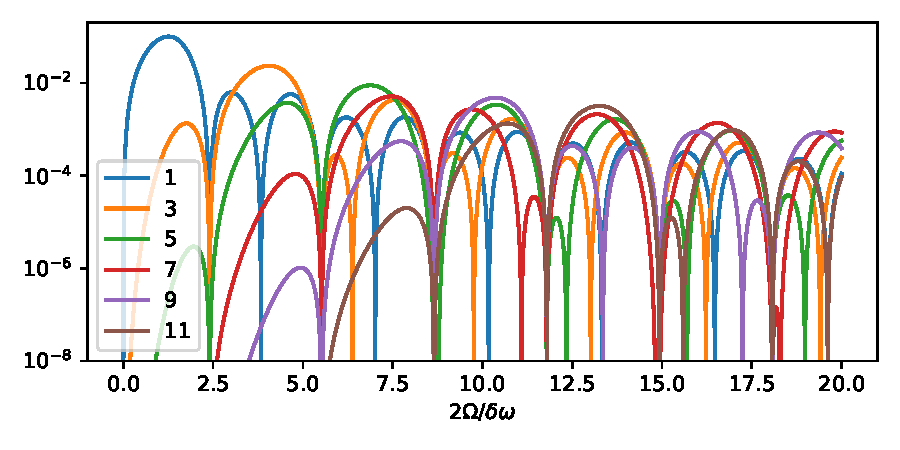
\includegraphics[width=0.95\textwidth]{zeros}
	\caption[Зависимость компонент эластичного рассеяния $I^{2l+1}(2\Omega/\delta\omega)$ для бихроматической накачки.]{Зависимость интенсивности компоненты эластичного рассеяния $I^{2l+1}(2\Omega/\delta\omega)$ для случая бихроматической накачки.}
	\label{fig: zeros}
\end{figure}
Подобную картину можно получить и при помощи рассмотрения одетого атома, однако в вышеупомянутых работах не приводится конкретных результатов для эластичного спектра, полученных на основе этого подхода. 

Мы рассмотрели известные теоретические и экспериментальные результаты для рассеяния бихроматического света на двухуровневой системе. По результатам рассмотрения можно отметить, что в данной работе впервые осуществляется систематическое экспериментальное исследование эластичного рассеяния: ранее в рамках традиционной оптики данный аспект изучался только теоретически, а известные экспериментальные работы \cite{Chakmakjian:88,Zhu_experiment} имеют дело только с неэластично рассеяным излучением. При этом, с точки зрения теории отдельно не рассматривался режим, в котором отстройка компонент драйва от резонанса кубита пренебрежимо мала по сравнению с излучательной шириной кубита.  Рассмотрев известные результаты, мы переходим к выполнявшимся в рамках работы экспериментам по рассеянию бихроматического света на одиночном сверхпроводящем кубите.
\section{Спектр эластичного рассеяния в случае $\delta \ll \Gamma_1$}
Исследование нелинейного рассеяния на одиночном кубите резонно начать с приложения к кубиту двух непрерывных волн. В рамках микроволновой техники наиболее просто использовать в качестве драйва выходные сигналы фазостабильных СВЧ-генераторов. В лаборатории искусственных квантовых систем для этого используются модели Keysight MXG N8257B и EXG N5283. Эти модели обеспечивают перестройку частоты в пределах до 20 ГГц, относительную аппаратную ширину линии порядка $10^{-11}$ и могут быть частотно синхронизированы друг с другом с такой же точностью. Кроме того, в качестве источника может использоваться и выход ВАЦ Keysight PNA-L, обладающий схожими характеристиками, но имеющий в качестве недостатка слабое подавление гармоник исходного синусоидального сигнала --- впрочем, этот эффект не является критическим для использования в обсуждаемом эксперименте. Для того, чтобы завести два непрерывных сигнала с различных источников в единый волновод, достаточно использовать СВЧ-делитель (splitter или power combiner) перед входом сигнала в криостат, объединенный выход которого направляется на вход криостата. Включение одного из источников позволяет произвести стандартные измерения однотоновой спектроскопии, зависимости линии кубита от мощности и резонансной флуоресценции, результаты которых рассматривались в разделах \ref{sec: spectr}-\ref{sec: Triplet_meas}. Нас же интересует спектр рассеянного на кубите сигнала, состоящего из двух компонент от разных источников.

Для решения поставленной задачи по измерению спектра эластичного рассеяния выход волновода с кубитом подключается к спектральному анализатору.  Зная естественную ширину его линии $\Gamma_1$, мы выбираем центральную частоту драйва $\omega_d$ близкую к частоте $\omega_q$ и устанавливаем на СВЧ-генераторах частоты $\omega_\pm = \omega_d \pm \delta\omega$, где величина отстройки $\delta\omega$ много меньше $\Gamma_1$, поскольку мы хотим остаться в резонансном приближении. Установив частоты, мы выравниваем мощности сигналов и начинаем синхронно увеличивать Раби амплитуды драйвов $\Omega_+ = \Omega_- = \Omega$, снимая получающийся спектр. При этом полоса входного фильтра спектрального анализатора может быть выбрана на уровне нескольких Гц, поскольку мы хотим максимально убрать шум и увидеть только эластичную часть сигнала, спектральная ширина которой очень мала.
\begin{figure}[thb]
	\centering
	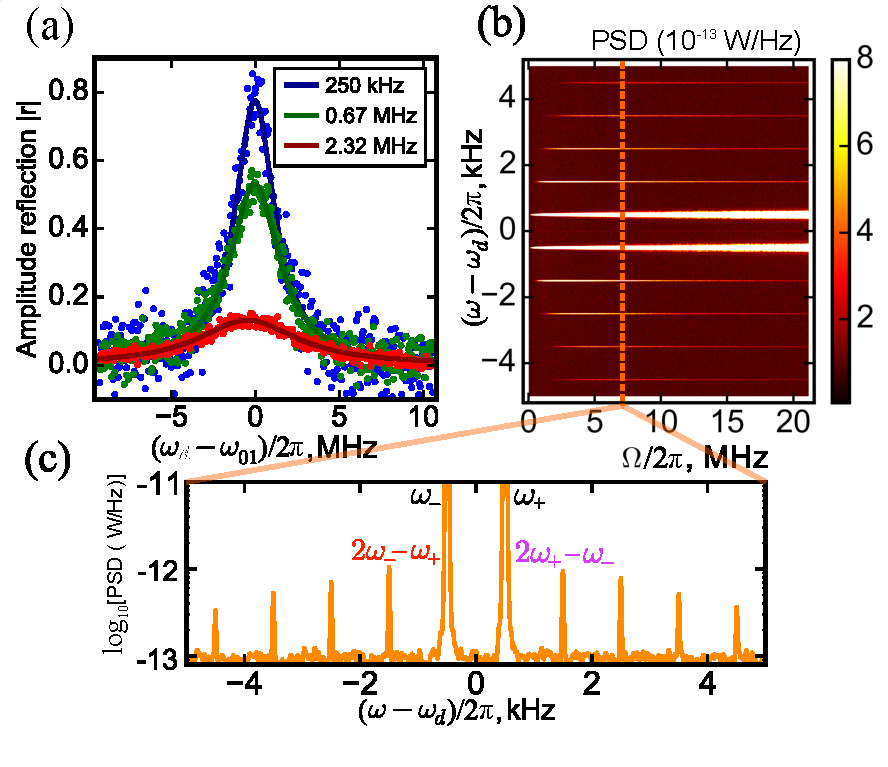
\includegraphics[width=0.85\textwidth]{Fig_2_fixed_PRA_forThesis.pdf}
	\caption[Волновое смешение: появление дополнительных компонент эластично рассеянного сигнала]{(a) Коэффициент прохождения $S_{21}$ одиночной резонансной волны на кубите в зависимости от отстройки $\Delta\omega = \omega_d-\omega_q$, при различных значениях частоты Раби. Параметры кубита $\Gamma_1/2\pi = 2.2$~МГц, $\Gamma_2 = \Gamma_1/2$. (b) Цветовой график спектров рассения двух волн на частотах $\omega_{\pm}$ в зависимости от частоты Раби для $\delta\omega = 1$ kHz. (c) Пример спектра при $\Omega/2\pi=7$~МГц. }
	\label{fig: CWM}
\end{figure}
Результаты измерений приведены на Рис.~\ref{fig: CWM}. Качественное поведение спектра по мере увеличения $\Omega$ хорошо проиллюстрировано на Рис.~\ref{fig: CWM}b). При увеличении Раби-частоты от нуля до нескольких единиц $\Gamma_1$ появляется большое количество эластичных пиков, частоты которых равны $\omega_{\pm(2p+1)} = (p+1)\omega_\pm-p\omega_\mp$ и интенсивности которых достигают своего максимума при определенных значениях $\Omega$, а в дальнейшем плавно спадают, см.  Рис.~\ref{fig: CWM}с). Таким образом, экспериментально показан эффект волнового смешения непрерывных волн на одиночной нелинейности в волноводе. В данном измерении на пути сигнала не имеется никаких нелинейных элементов, которые мы могли бы вызвать подобное рассеяние. В качестве подтверждения, аналогичные измерения были проведены при большой отстройке кубита $\Delta\omega = \omega_q - \omega_d \gg \Gamma_1 $, и в этом режиме не было обнаружено дополнительных спектральных компонент. Таким образом, можно считать доказанным факт наблюдения волнового смешения на одиночном сверхпроводящем атоме в волноводе.  

В режиме непрерывной бихроматической накачки интерес представляет снятие зависимости компонент напряжения, отвечающих дополнительным спектральным линиям, от частоты Раби $\Omega$, и сопоставление  полученного результата с аналитическим расчетом. Более того, поскольку имеется возможность менять $\Omega_+$ и $\Omega_-$ независимо, представляет интерес показать, как меняется в этом случае вид спектра эластичного рассеяния. Как будет показано в следующем разделе, для расчета спектра в режиме $\delta\omega \ll \Gamma_1$, в котором проводятся практически все излагаемые ниже измерения, можно воспользоватся аналитическим выражением \eqref{eq: refl} для поля, излучаемого кубитом в стационарном режиме в случае монохроматического драйва и получить выражения для амплитуд напряжений и мощностей боковых компонент поля $\Omega_{\pm(2p+1)}$, выраженных в единицах частоты Раби. Физический смысл этих компонент следует из соотношения $\hbar\Omega_{\pm(2p+1)} = \mu V_{\pm{2p+1}}$. Также мы проведем сравнение полученных формул с экепериментальными данными и обсудим потенциальные применения данного эффекта.

\section{Аналитическое выражение для амплитуд боковых гармоник в приближении малой отстройки}
\label{sec: anal_sol}

Для расчета амплитуд дополнительных гармоник, появляющихся в результате волнового смешения, запишем гамильтониан для двухуровневой системы, дипольно связанной с континуумом мод волновода, в котором распространяется вышеупомянутое бихроматическое поле. Гамильтониан имеет следующий вид:
\begin{equation}	
H = -\frac{\hbar \omega_{01}}{2}\sigma_z -\hbar \Omega_- \sigma_x \cos(\omega_d t - \delta\omega t) -\hbar \Omega_+ \sigma_x \cos(\omega_d t + \delta\omega t),	
\end{equation} 
где $\Omega_+$ и $\Omega_-$ определены выше. Для начала мы рассчитаем стационарное решение основного квантового уравнения для данного гамильтониана в приближении вращающейся волны. Член  $\delta\omega t$, стоящий под знаком косинуса, будет рассматриваться здесь как медленно меняющаяся во времени фаза, потому что  $\delta\omega t \ll 1$ на масштабе времени когерентности $t \sim \Gamma_2^{-1}$ кубита. Аналитическое решение для среднего значения оператора понижения для атома имеет вид:  
\begin{equation}
\langle \sigma^-\rangle = -\frac{\sin\theta}{\Lambda} \frac{\Omega_- e^{-i\delta\omega t} + \Omega_+ e^{i \delta\omega t}}{1 + \sin\theta\cos{2\delta\omega t}}. 
\label{exp_value}
\end{equation}
%Here we introduce the following notations: $\frac{1}{\Lambda} = \frac{\Gamma_1 \lambda}{2D}$, $\beta = \frac{2\Gamma_2 \Omega_- \Omega_+}{D}$, where $\lambda = \Delta \omega - i\Gamma_2$, $D = \Gamma_1 |\lambda|^2 + \Gamma_2(\Omega_-^2 + \Omega_+^2)$.
Здесь введены следующие обозначения: $\theta = \arcsin\Big(\frac{2\Gamma_2 \Omega_- \Omega_+}{\Gamma_1 |\lambda|^2 + \Gamma_2(\Omega_-^2 + \Omega_+^2)}\Big)$, $\Lambda^{-1} = \frac{\lambda\Gamma_1}{4\Gamma_2 \Omega_-\Omega_+}$, $\lambda = \Gamma_2 + i\Delta\omega$.
%\begin{align*}
%A = \frac{\Gamma_1 \lambda}{2D}, 
%\beta & = \frac{2\Gamma_2 \Omega_- \Omega_+}{D}, \lambda = \Delta \omega - i\Gamma_2, \\
%D & = \Gamma_1 |\lambda|^2 + \Gamma_2(\Omega_-^2 + \Omega_+^2).
%\end{align*} 
Знаменатель уравнения~\eqref{exp_value} можно переписать согласно соотношению  
\begin{equation}
%\langle \sigma^-\rangle = \frac{\Omega_- e^{-i\delta\omega t} + \Omega_+ e^{i \delta\omega t}}{\alpha \Lambda} \sum_{p=-\infty}^{\infty}y^{|p|} e^{i 2 p \delta\omega t},
\frac{1}{1+\frac{1}{2}\sin\theta(z + z^{-1})} = \frac{1}{\cos{\theta}}\Big(\frac{1}{1- yz} + \frac{1}{1- yz^{-1}}-1\Big), 
%\frac{1}{\cos{\theta}}\sum_{p=-\infty}^{\infty}y^{|p|} e^{i 2 p \delta\omega t},
\label{exp_value2}
\end{equation}
где %$\beta = \frac{y}{1+y^2}$ and $z = e^{2i\delta\omega t} $ 
$z = e^{2i\delta\omega t}$ и $y = -\tan{\frac{\theta}{2}}$. Правая часть уравнения \eqref{exp_value2} раскладывается в степенной ряд по $z$ и мы получаем:
\begin{equation}
%\langle \sigma^-\rangle = \frac{\Omega_- e^{-i\delta\omega t} + \Omega_+ e^{i \delta\omega t}}{\alpha \Lambda} \sum_{p=-\infty}^{\infty}y^{|p|} e^{i 2 p \delta\omega t},
\langle\sigma^-\rangle = -\frac{\Omega_- e^{-i\delta\omega t} + \Omega_+ e^{i \delta\omega t}}{\Lambda}\tan\theta \sum_{p=-\infty}^{\infty}y^{|p|} e^{i 2 p \delta\omega t}.
\label{exp_value3}
\end{equation}
Учитывая, что  $\hbar V_{sc} = -i\Gamma_1\!\braket{\sigma_-}\!/\mu$ и преобразуя сумму к неотрицательным $p$, мы получаем:
\begin{equation}
V^{sc} =  
-\frac{\hbar\Gamma_1\tan\theta}{\mu\Lambda}\sum_{p=0}^{\infty}y^p\Big[ (\Omega_- + y \Omega_+ ) e^{-i(2p+1)\delta\omega t}
+ (y \Omega_- + \Omega_+) e^{i(2p+1)\delta\omega t}\Big].
\label{an_eq}
\end{equation}
Учитывая соотношения $V_\pm \mu = \hbar\Omega_\pm$, мы можем записать результат для Раби-амплитуд дополнительных спектральных компонент, появившихся в результате рассеяния на атоме: 
\begin{equation}
%|\Omega_{\pm(2p+1)}^{sc}|^2 =\left[\frac{\Gamma_1 A}{\alpha} y^{p}(\Omega_{\mp}+y\Omega_{\pm})\right]^2,
\Omega_{\pm(2p+1)}^{sc} =\frac{(-1)^p\Gamma_1\tan\theta\tan^p\frac{\theta}{2}}{\Lambda} (\Omega_{\mp}\tan\frac{\theta}{2} - \Omega_{\pm}),
\label{intensities}
\end{equation} 
которое можно проверить, измеряя интенсивности компонент в эксперименте.

\begin{figure}[thb]
	\centering
	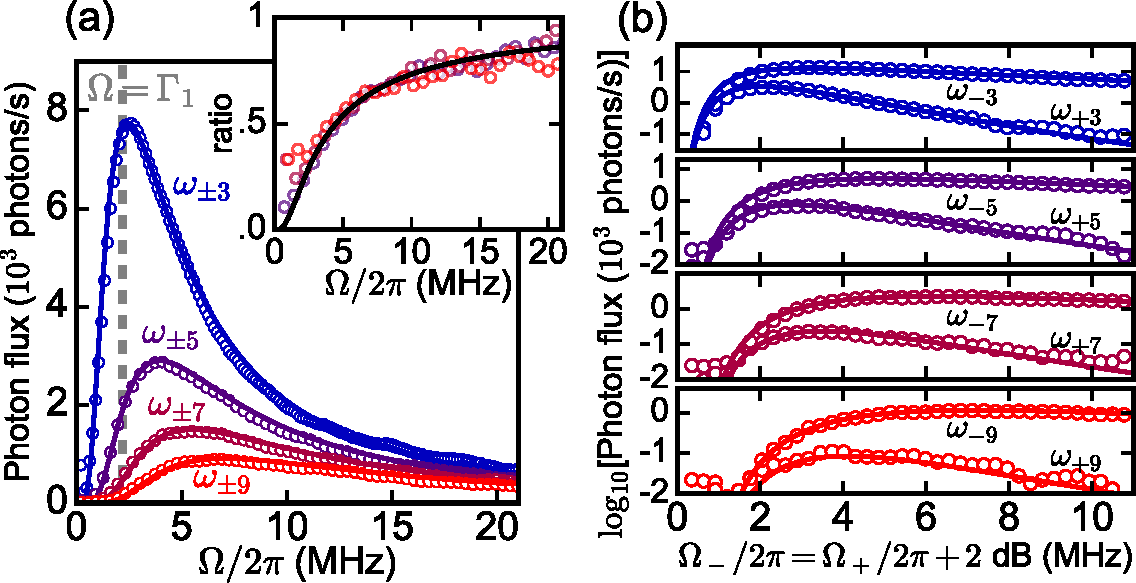
\includegraphics[width=0.9\textwidth]{Fig3_PRA_proofs3.pdf}
	\caption[Эластичные компоненты: сравнение аналитического расчета и экспериментальных результатов ]{(a) Боковые спектральные компоненты эластично рассеянного излучения, выраженные в единицах потока фотонов. Экспериментальные данные получены для $\delta\omega/2\pi=5$~кГц сравниваются с результатом в соответствии с  \eqref{intensities} (сплошные линии) с параметрами $\Gamma_1/2\pi = 2.2$~МГц, $\Gamma_2/2\pi=1.1$~МГц, $\Delta\omega/2\pi=0$, $\Omega_+=\Omega_- =\Omega$ и $p=1,2,3,4$ для каждой из кривых, соотвественно. На вставке приведены отношения потоков для последовательных порядков $2p+1$ и $2p+3$ для $p=1,2,3$. Черная линия представляет прямой расчет отношений согласно \eqref{intensities}. (б) Компоненты волнового смешения при ассимметричном драйве: $\Omega_-$~ на 2 дБ превышает $\Omega_+ $. Поток фотонов в компонентах с отрицательной стороны в несколько раз превышает поток в соответствующих положительных компонентах. Это свидетельствует о высокой чувствительности компонент волнового смешения к неравенству амплитуд сигналов бихроматической накачки.}
	\label{Peaks_WM_with_fit}
\end{figure}

На Рис.~\ref{Peaks_WM_with_fit} проводились измерения интенсивностей спектральных компонент в зависимости от $\Omega_-, \Omega_+$, и результаты этих измерений сравнивались с выражением \eqref{intensities} без применения подгоночных параметров. Рис.~\ref{Peaks_WM_with_fit}(a) представляет потоки фотонов в компонентах для  $1< p < 4$ (вплоть до 9-фотонных процессов) в случае $\Omega_+\!=\!\Omega_-\!=\!\Omega$ как функцию $\Omega$: правые и левые боковые пики в этом случае имеют равные амплитуды. С увеличением $\Omega$, амплитуды боковых пиков достигают максимума и потом уменьшаются, причем по мере увеличения $p$ максимум компоненты соотвествующего порядка достигается при большем значении $\Omega$. Это можно интерпретировать, считая, что порядок компоненты $2p + 1$ соответствует числу взаимодействующих на кубите фотонов из исходных сигналов на частотах $\omega_+, \omega_-$. Скорость испускания и поглощения фотонов определяется частотой Раби, а характеристическое время взаимодействия с кубитом определяется его когерентностью $\tau \sim \Gamma_2$. Поэтому, для эффективного поглощения или излучения фотонов в боковой пик порядка $\pm(2p+1)$ необходимо выполнить условие
\begin{equation}
2\Omega\cdot \tau \approx 2p+1,
\end{equation}
откуда получаем качественную оценку $\Omega_{max} \approx \Gamma_1(2p+1)/4$. Анализируя выражение \eqref{intensities} на предмет экстремума, получаем точные значения максимумов $\Omega_{max} = \sqrt{2} \Gamma_1(2p+1)/4$, что согласуется с физической картиной, которую мы приводим в качестве объяснения наблюдаемых эффектов. Дополнительно отметим, что уравнение \eqref{intensities} показывает, что зависимость спектральной компоненты от порядка смешения $p$ определяется лишь сомножителем $\tan^p\frac{\theta}{2}$. Чтоб дополнительно проиллюстрировать этот факт, мы рассчитываем отношения последовательных компонент порядка $2p+1$ и $2p+3$ для данных на Рис.~\ref{Peaks_WM_with_fit}(a) для $p=1,2,3$. Отметим, что результат не зависит от $p$ и хорошо согласуется с теорией. Это отчасти напоминает тот факт, что пуассоновское распределения фотонов в классическом когерентном состоянии полностью задается первым моментом, то есть, математическим ожиданием. Поэтому мы можем ожидать, что данное свойство равенства отношений не будет выполняться для квантовых когерентных полей с субпуассоновским или суперпуассоновским распределением фотонной статистики. Более подробное внимание этому вопросу уделяется в разделе \ref{sec: mix_stat}.

В следующем разделе мы опишем динамику кубита, и как следствие, спектр эластичного рассеяния для случая произвольного соотношения между $\Gamma_1$ и $\delta\omega$ при помощи численного решения уравнения Максвелла-Блоха для бихроматической накачки.    

\section{Численное решение уравнений Максвелла-Блоха}
\label{sec: maxbloch_num}
В предыдущем разделе мы вывели аналическое решение блоховских уравнений для случая $\delta\omega \ll \Gamma_1$. Сейчас мы хотим рассмотреть в дополнение к аналитическому решению численное решение приведенных уравнений. Имеет смысл сделать это по двум причинам. Во-первых,  аналитический ответ не работает при $\delta\omega \ge \Gamma_1$, так как в этом случае некорректно рассматривать множители $\delta\omega t$ как медленно меняющуюся фазу. Во-вторых, численное решение позволит не только узнать стационарное состояние системы, но также визуализировать динамику кубита до затухания, тогда как аналический ответ дл динамики может быть слишком сложен. 

\begin{figure}[h]\label{fig: num_bich}
\centering
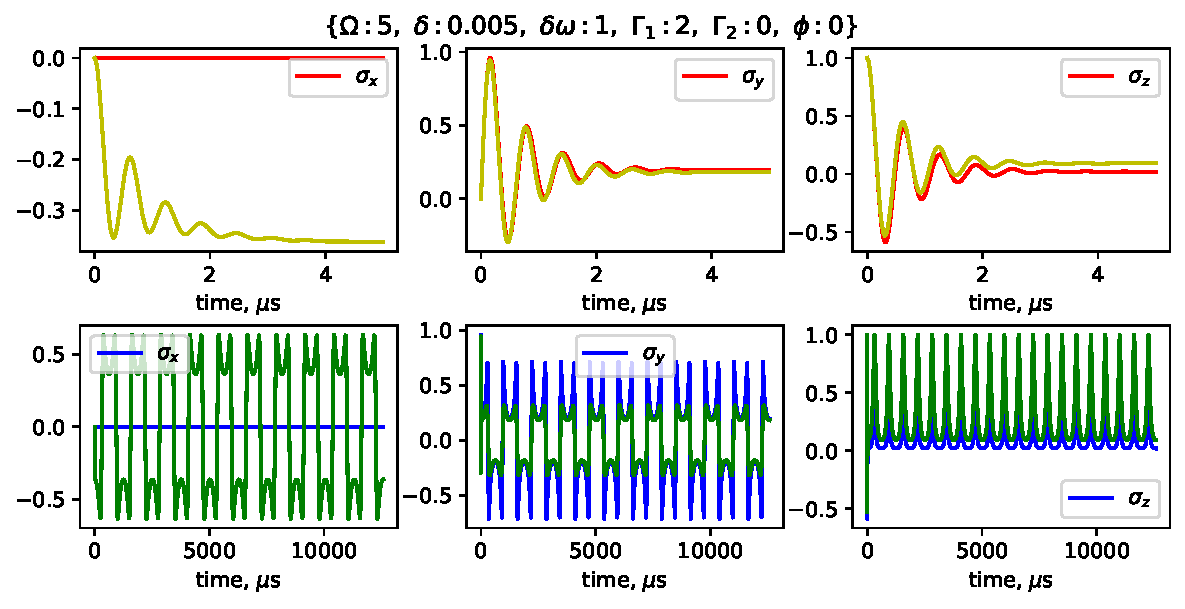
\includegraphics[width=0.9\textwidth]{2drives_num.pdf}
\caption[Численное решение уравнений Блоха для двухуровневой системы для случая бихроматической накачки]{Средние значения атомных операторов в зависимости от времени, полученные при помощи численного решения уравнений \eqref{eq: bloch_bich}. Численные значения параметров (МГц) указаны в заголовке рисунка. Верхний ряд графиков показывает динамику кубита до затухания, а нижний ряд --- дрейф стационарного состояния за счет отстройки. На каждом из графиков пара кривых соотвествует значениям $\Delta\omega=0$~МГц (красная и синяя линии) и $\Delta\omega=1$~МГц (желтая и зеленая линии).}
\end{figure}
\begin{figure}[t]\label{fig: bloch_num_bich}
	\centering
	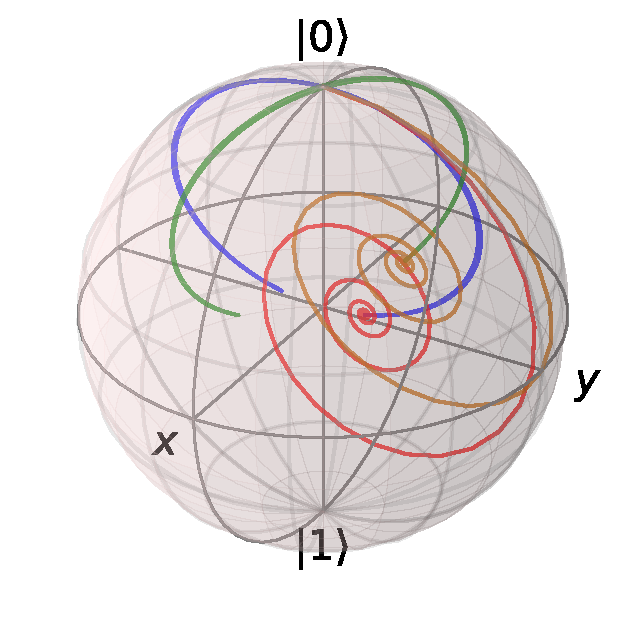
\includegraphics[width=0.6\textwidth]{bloch_2drives_num.pdf}
	\caption[Представление численное решение уравнений Блоха для случая бихроматической накачки на сфере Блоха]{Отображение представленных на Рис.~\ref{fig: num_bich} кривых на сфере Блоха. Дрейф стационарного состояния представляет собой движение по некоторой плоской кривой, поворот которой меняется в зависимости от глобальной отстройки $\Delta\omega$.}
\end{figure}
Для симуляции динамики кубита можно использовать пакет \verb|QuTiP|, реализующий широкий спектр расчетов с квантовыми объектами на базе вычислительных библиотек языка программирования \verb|Python|. Основное квантовое уравнение решается при помощи функции \verb|mesolve|, которая также может рассчитать зависимость среднего значения указанных в аргументах операторов от времени. Как мы отмечали ранее, уравнения Блоха для случая бихроматической накачки имеют вид:
\begin{equation} \label{eq: bloch_bich}
	\dot{\boldsymbol{\sigma}} =\mathbf{M}_b\cdot \boldsymbol{\sigma} + \mathbf{B},
\end{equation} где $\mathbf{B} = [0,\quad 0, \quad-\Gamma_1]^{T}$, a матрица $\mathbf{M}_b$ имеет вид:
\begin{equation}\label{eq: bloch_bich}
	\mathbf{M}_b = \left[\begin{matrix}- {\Gamma}_{2}  & 0 & - 2 \Omega \cos{\left(\delta\omega t + \phi \right)}\\0 & - \Gamma_{2} & - 2 i \Omega \cos{\left(\delta\omega t + \phi \right)}\\\Omega \cos{\left(\delta\omega t + \phi \right)} & - i \Omega \cos{\left(\delta\omega t + \phi \right)} & - \Gamma_1\end{matrix}\right]
\end{equation}
Численное решение этих уравнений приведено на Рис. \ref{fig: num_bich}, для параметров, соотвествующих приближению слабо отстроенных драйвов. Более информативно анализировать результат, построив графики на сфере Блоха, см. Рис.~\ref{fig: bloch_num_bich}. Динамика кубита качественно не отличается от случая однотоновой резонансной накачки, но появляется дрейф стационарного состояния за счет медленно меняющейся фазы. Если мы увеличим отстройку частот накачки, то динамика становится более насыщенной, и вместо стационарного состояния решение более похоже на незатухающую динамику с некоторыми метастабильными точками, возле которых состояние задерживается дольше. 
\begin{figure}[t]\label{fig: bloch_num_bich2}
	\centering
	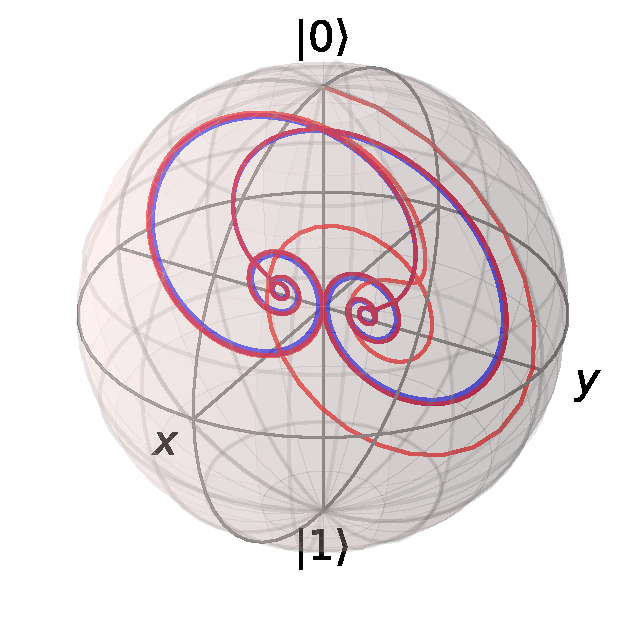
\includegraphics[width=0.6\textwidth]{bloch_2drives_num2.pdf}
	\caption[Численное решение уравнений Блоха для случая бихроматической накачки на сфере Блоха, для случая $\delta\omega \approx \Gamma_1$]{Решение уравнений Блоха при $\delta\omega=0.7$~МГц, остальные параметры совпадают со значениями для кривых на Рис.~\ref{fig: num_bich}. Красная линия отражает начальный этап динамики, синяя --- демонстрирует динамику после стабилизации.}
\end{figure}
В разделе \ref{sec: anal_sol} показано, что волновое смешение можно получить из разложения в спектр поля, которое излучается в слабо менябщемся  квазистационарном состоянии с переменной фазой. Имея численное решение, мы можем получить аналогичный результат при взятии численного преобразования Фурье. Результат изображен на Рис.~\ref{fig: mix_fft} и количественно совпадает с экспериментальными данными на Рис.~\ref{fig: CWM}с). Аналогично можно расчитать, например, зависимость боковых компонент от $\Omega$, и также получить хорошее количественное  совпадение с экспериментом, см. Рис. \ref{fig: mix_fft_omega}.
\begin{figure}[t]\label{fig: mix_fft}
	\centering
	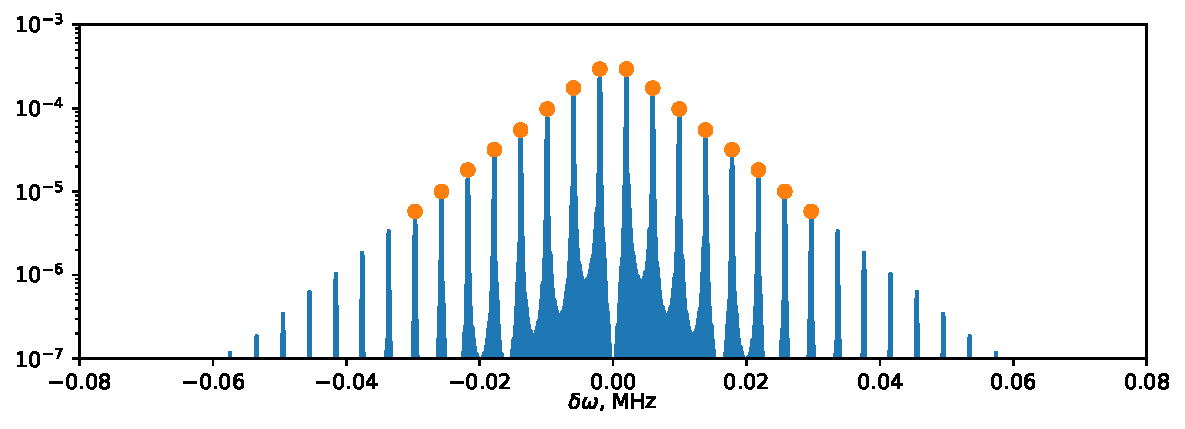
\includegraphics[width=0.99\textwidth]{fft_spec.pdf}
	\caption[Компоненты смешивания волн, полученные как спектр поля, излучаемого в стационарном состоянии]{Компоненты смешивания волн, полученные как спектр поля, излучаемого в стационарном состоянии. Параметры решения приведены в заголовке к Рис.~\ref{fig: num_bich}.}
\end{figure}
\begin{figure}[t]\label{fig: mix_fft_omega}
	\centering
	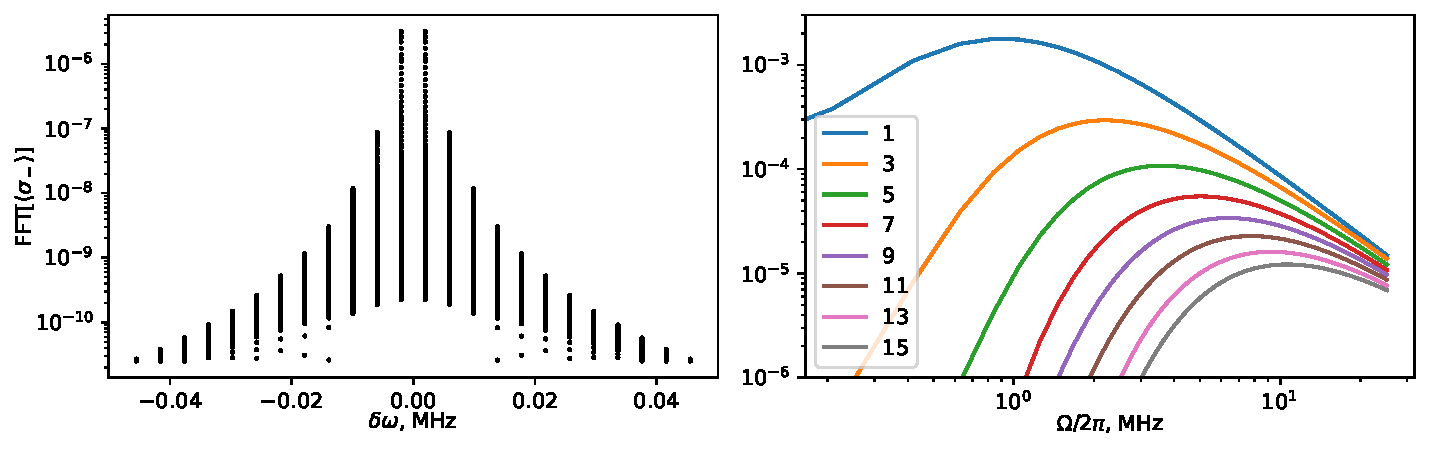
\includegraphics[width=0.99\textwidth]{mixing_Omega.pdf}
	\caption[Зависимость дополнительных компонент от Раби частоты двух управляющих сигналов]{Зависимость дополнительных компонент от Раби частоты $\Omega = $ двух управляющих сигналов, полученная как Фурье-спектр численного решения уравнений Блоха. Слева: значения компонент поля при всех исследуемых $\Omega$. Справа: зависимость компонент различных порядков от $\Omega$.  Параметры решения приведены в заголовке к Рис.~\ref{fig: num_bich}.}
\end{figure}

В данном разделе мы показали, что численное решение уравнений Блоха хорошо описывает эксперимент по смешению бихроматической накачки на кубите. В дальнейшем мы используем этот факт для интерпретации измерений спектра когерентного рассеяния при импульсной бихроматической накачке, когда получение точного аналитического решения более затруднительно.
 
\section{Расщепление Аутлера-Таунса для боковых компонент}
Еще один любопытный эффект, наблюдаемый при измерении когерентной части рассеиваемого кубитом поля --- расщепление интенсивности компонент при изменении глобальной отстройки $\Delta\omega$ между частотой кубита и центральной частотой накачки. Матрица $\mathbf{M}_b,$ задающая уравнения Блоха вида \eqref{eq: bloch_bich}, имеет вид:
$$
\mathbf{M}_b = \left[\begin{matrix}- \Gamma_2 & i \Delta\omega & - 2 \Omega \cos{\left(\delta\omega t + \phi \right)}\\i \Delta\omega & - \Gamma_{2} & - 2 i \Omega \cos{\left(\delta\omega t + \phi \right)}\\\Omega \cos{\left(\delta\omega t + \phi \right)} & - i \Omega \cos{\left(\delta\omega t + \phi \right)} & - \Gamma_1\end{matrix}\right],
$$
\begin{figure}[th]\label{fig: autler-townes like}
	\centering
	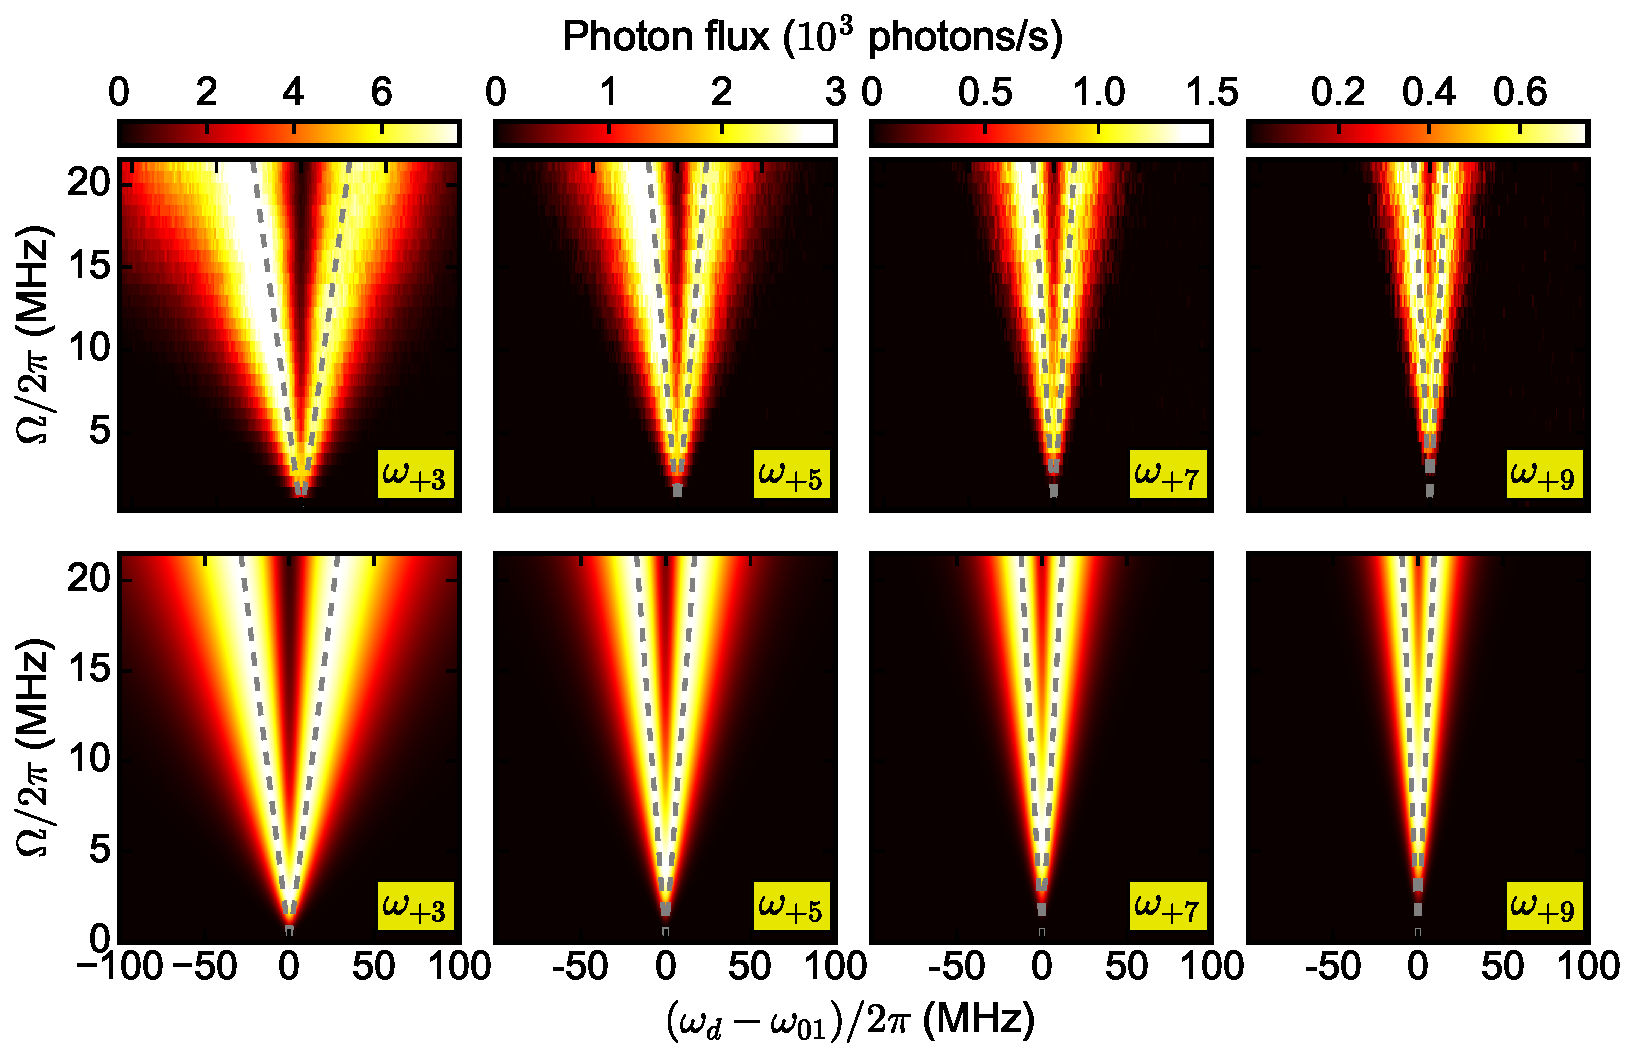
\includegraphics[width=0.95\textwidth]{Fig4_PRA_proofs2.pdf}
	\caption[Расщепление Аутлера-Таунса боковых компонент эластичной части рассеянного на кубите сигнала.]{Расщепление Аутлера-Таунса, наблюдаемое при измерении компонент различного порядка в эластичной части рассеянного на кубите сигнала в зависимости от $\Delta\omega$ и $\Omega$. Верхний ряд графиков представляет измеренные значения $\Omega_{\pm(2p+1)}^{\text{sc}}$, пересчитанные в единицы потока фотонов при помощи выражения \eqref{eq: av_photons}. Нижние панели представляют собой результаты аналитических расчетов согласно \eqref{intensities}. Серые пунктирные линии --- направляющие, соответствующие $\delta\omega = \pm 4\Omega/(2p+1)$. }
\end{figure}
а значение компонент $\Omega_{\pm(2p+1)}^{\text{sc}}$ все так же описывается уравнением \eqref{intensities}. Для измерения зависимостей $\Omega_{\pm(2p+1)}^{\text{sc}}(\Delta\omega)$ не требуется дополнительных технических усложнений: достаточно лишь учесть, что все частоты $\omega_{\pm(2p+1)}$ смещаются также на величину $\Delta\omega$, тогда как частота кубита остается на месте. Результаты измерения этих зависимостей и их сравнения с аналитическими значениями приведены на Рис.~\ref{fig: autler-townes like}. Видно, что с увеличением частоты Раби в эластичной компоненте каждого порядка возникает два расходящихся максимума, расстояние между которыми зависит от порядка спектральной компоненты и хорошо определяется как 
\begin{equation}\label{ATS-like}
	2\Delta\omega = 8\Omega/(2p+1). 
\end{equation}

Полученное расщепление напоминает по своей структуре расмотренный в разделе \ref{AT} эффект Аутлера-Таунса, где расщепление пиков в прохождении резонансного пробного сигнала малой амплитуды является следствием сильной накачки одного из переходов в трехуровневой системе. Однако, имеется ряд существенных различий: система является двухуровневой и мы не прикладываем дополнительный пробный сигнал. Можно предположить, что сильная бихроматическая накачка в сочетании с ненулевой отстройкой создает сложную систему одетых состояний, и переходы между этими состояниями вызывают наблюдаемые картины интенсивностей боковых компонент. Однако, детальный аналитический расчет когеретных компонент с иcпользованием одетых уровней может быть достаточно сложен и до сих пор не встречался в литературе: например, в работе \cite{Ficek_resonance} уравнения решаются численно, но не ставится задача нахождения аналитического решения. Поэтому количественно точное описание расщеплений при помощи системы одетых уровней, бесспорно, являясь крайне интересной физической задачей, тем не менее, выходит за рамки представляемой работы.
\section{Волновое смешение и фотонная статистика в волноводе}
\label{sec: mix_stat}
Как было указано в разделе \ref{sec: maxbloch_num}, волновое смешение может быть использовано в качестве инструмента изучения фотонной статистики в некоторой волноводной моде. В микроволновом диапазоне частот это приобретает особенное практическое значение ввиду отсутствия эффективных детекторов фотонов, и как следствие, техническими сложностями при измерении корреляционной функции поля второго порядка $G^{(2)}(t, \tau)$, которая является общепризнанным стандартным измерением, позволяющим установить квантовость (в частности, однофотонность) распространяющегося поля) и даже выполнить полную томографию поля \cite{Eichler_tomo, EichlerTomography}. Мы можем проиллюстрировать возможность исследования фотонной статистики, опираясь на полученные в данном разделе результаты.

Для иллюстрации возможности восстановления статистики подсчитаем среднее число фотонов в интересующей нас моде, пролетающее мимо кубита на характерном времени $\tau\sim\Gamma_2^{-1}$). Мы выбираем масштаб, отвечающий времени когеретности кубита, поскольку характеризуем именно эластичное рассеяние, для которого важен тот факт, что состояние кубита не потеряло информацию о фазе. Поэтому среднее число фотонов равно $\braket{N} = P(\hbar\omega\Gamma_2)^{-1}$. Мощность излучения в линии можно выразить через амплитуду раби $\Omega$: $P = (\hbar\Omega/\mu)^2/(2Z_0)$. Комбинируя эти выражения с \eqref{eq: G1}, получаем:
\begin{equation} \label{eq: av_photons}
	\braket{N} = \frac{\Omega^2}{\Gamma_1\Gamma_2}.
\end{equation}
Для простоты рассмотрим предел слабой накачки: $\Omega_{\pm} \gg \Gamma_1.$ В этом приближении легко показать, что:
$\theta \approx (\Omega_+\Omega_-)/\Gamma_2^2, \Lambda \approx (2\Omega_+\Omega_-)/{\Gamma_2}
$. При подстановке в \eqref{intensities} получаем:
\begin{equation}\label{eq: 2p+1_approx}
	\Omega_{\pm(2p+1)}^{sc} =\frac{(-1)^{p+1}}{2^{p}}\Gamma_2^{-2p-1}\Gamma_1\Omega_+^{p+1}\Omega_-^p,
\end{equation}
В результате, амплитуда боковой компоненты зависит от степеней апмлитуд исходных полей, показатели которых соответствуют порядку нелинейности. Поэтому и средние числа фотонов подчиняются схожему соотношению:
\begin{equation}\label{eq: N_2p+1}
	\braket{N_{2p+1}} = \braket{N_-}^p\braket{N_+}^{p+1}
\end{equation}
Это полуклассическое рассуждение наводит нас на мысль о том, что среднее число фотонов может не только зависеть от средних $\braket{N_+},\!\braket{N_-}$, но и содержать в себе более подробную информацию о фотонной статистике. Естественно, это предположение невозможно подтвердить для пуассоновских распределений фотонов, для которых первый момент определяет все последующие. Однако, многофотонная природа процессов волнового смешения является сильным аргуменом в пользу того, что интенсивности вновь появляющихся в результате волнового смешения пиков должны быть чувствительны к индивидуальным амплитудам вероятности фоковских состояний в исходных модах $\omega_\pm$ или к каким-либо комбинациям этих амплитуд. Переходя к квантовомеханическому описанию поля, выражение в правой части \eqref{eq: N_2p+1} можно получить также как среднее значение оператора $(a_+a_-^\dag)^pa^+$ на когерентных состояний в двух модах $\ket{\alpha_+, \alpha_-}$ На основе эксперимента с классической накачкой доказать его справедливость невозможно, однако, весьма похожий эффект теоретически рассматривался в работах \cite{WallsMilburn_PRD,PhysRevA.28.2646}. В этих работах изучались различные способы измерения интересующего исследователя квантового объекта, а именно --- гармонического осциллятора с полем $\hat{a}$. В качестве измерителя выступает другой осциллятор $\hat{b}$, испытывающий значительное воздействие со стороны окружения. Считается, что объект взаимодействует с измерителем таким образом, что гамильтониан этого взаимодействия имеет вид:
\begin{equation}
	H_{m-o} = \frac{\hbar}{2}a^\dag a(\Omega b + \Omega^* b^\dag),
\end{equation}
и как утверждается, может быть реализован через волновое смешение на нелинейной восприимчивости третьего порядка. В свою очередь, измеритель отдает свою энергию окружению, состоящему из большого числа осцилляторов:
\begin{equation}
	H_{B-m} = \sum_i^{}\kappa_i\left(B_ib^\dag +B^\dag_i b\right).
\end{equation}
В работе \cite{WallsMilburn_PRD} показано, что в этом случае результирующее состояние системы из двух осцилляторов позволяет осуществить неразрушающее измерение изучаемого объекта в фоковском базисе, при этом стабильный базис измерителя состоит из когерентных состояний и измерение может быть рассмотрено в классическом пределе. Система при этом считается бесконечно долгоживущей, так как нас интересует лишь процесс измерения. Говоря точнее, если задано начальное состояние системы <<объект-измеритель>>:
\begin{equation}
	\rho(0) = \sum_{n,m}^{}\rho_{n,m}(\ket{n}\bra{m})_o\otimes(\ket{0}\bra{0})_m,
\end{equation}
то после затухания когерентности в измерителе состояние стремится к:
\begin{equation}
	\lim_{t \to \infty}\rho(t) = \sum_n^{}\rho_{nn} (\ket{n}\bra{n})_m \otimes
	(\ket{\alpha_n}\bra{\alpha_n})_o,
\end{equation}
где $\alpha_n = \Omega n (1-e^{\gamma t/2})/\gamma$, а $\gamma$ --- скорость релаксации измерителя в окружение. Таким образом, если спроецировать измеритель на когерентное состояние, то объект окажется в фоковском состоянии. Также показано, что если накапливать отсчеты детектора фотонов, проецирующего состояние измерителя, то полное число отсчетов при условии быстрого измерения и сильной связи с полем $\Omega$ пропорционально $\braket{a^\dag a}^2$. Эти результаты подтверждают выдвинутые предположения о применимости наблюдаемого эффекта для измерений числа фотонов в распространяющихся мимо кубита модах. 

Подводя итоги вышесказанному, продемонстрирован фундаментальный эффект волнового смешения стационарных когерентных состояний на одном двухуровневом рассеивателе, сильно связанном с одномерной линией передачи. Мы получили аналитическое выражение для амплитуд смешанных состояний и показали ряд других физических эффектов, например, подобное Аутлеру-Таунсу расщепление боковых пиков в зависимости от числа рассеянных фотонов. Боковые пики являются результатом процессов многофотонного рассеяния, а их амплитуды определяются распределением фотонов в когерентных состояниях. Интересным будущим применением будет визуализация статистики неклассических когерентных состояний. Использование волнового смешения сигналов на кубите для восстановления фотонной статистики этих сигналов может стать весьма перспективным применением полученных в данной работе результатов. Однако, это утверждение требует дополнительной экспериментальной проверки. В следующем разделе мы обратимся к импульсному драйву кубита в различных исполнениях и покажем, что спектр рассеяния импульсной накачки крайне чувствителен к разрешенным и запрещенным многофотонным процессам рассеяния, и модифицируется в соотвествии с числом фотонов, доступных для реализации того или иного процесса. 


 




           % Глава 3
\chapter{Двухчастотное волновое смешение в импульсном режиме}
\label{ch: q_mixing}

В данной главе будут описаны эффекты волнового смешения, возникающие при импульсной бихроматической накачке двухуровневой системы. В этих экспериментах на кубит подаются последовательности прямоугольных или близких к ним по форме импульсов. Несущие частоты этих последовательностей незначительно отстроены от резонанса кубита, длительности импульсов варьируются от $0$ до нескольких $T_1$ кубита, а промежутки между импульсами значительно превышают $T_1$. Качественная картина спектра эластичного рассеяния претерпевает значительные изменения по сравнению с непрерывной накачкой. Например, при рассеянии синхронизированных прямоугольных импульсов на частотах $\omega_{pm}$ наблюдается бесселевская динамика боковых компонент сигнала в зависимости от эффективной длительности импульса $\Omega\Delta t$. Совершенно новый физический эффект возникает при введении задержки между последовательностями импульсов. Длительность задержки должна превосходить длительность импульса для того, чтобы отдельные импульсы на частоте $\omega_+$ попадали на кубит раньше импульсов на частоте $\omega_-$ и не перекрывались с ними. При этом кардинально меняется вид спектра эластичного рассеяния. Вместо большого количества симметричных пиков мы наблюдаем лишь один дополнительный пик на частоте $2\omega_--\omega_+$. Этому эффекту можно дать простое качественное объяснение, напрямую вытекающее из свойства кубита поглощать не более чем единичный квант поля. В дополнение к этому, мы изучаем рассеяние последовательностей импульсов на трехуровневой эквидистантной системе, которая возникает при некотором значении внешнего магнитного потока, проходящего через петлю изучаемого нами потокового кубита. Помимо к двух компонент на исходных несущих частотах и одной компоненте от четырехволнового смешения, к эластичному спектру добавляется еще две компоненты, соотвествующие двухфотонным процессам, что подтверждает справедливость качественной интерпретации экспериментальных результатов. Последние два режима мы будем называть \textit{квантовым волновым смешением}, поскольку оно обладает рядом необычных свойств, обусловленных квантовостью сверхпроводникового искусственного атома. В дополнение к экспериментальным данным, в данном разделе проведен численный расчет спектра, согласующийся с экспериментом, а также дано строгое теоретическое обоснование трехпикового спектра рассеяния на двухуровневой системе и пятипикового спектра рассеяния на трехуровневой системе на основе формализма вторичного квантования.  
\section{Случай синхронных импульсов: бесселевская динамика}
\label{sec: bessels}
Для изучения импульсного смешения при помощи экспериментальной схемы \ref{fig: pulse_setup_1} необходимо запрограммировать генератор импульсов произвольной формы (AWG) так, чтобы на его выходе получить последовательность прямоугольных импульсов. Несущая частота этих импульсов $\omega_{\text{IF}}/2\pi$ может варьироваться от 0 до 100 МГц, а период импульсов $T\gg 1/\Gamma_1$ обеспечивает релаксацию кубита после импульса за время, предшествующее появлению следующего импульса. Длительности импульсов $\delta t$ также меняются произвольно, технические возможности AWG позволяют получить импульсы длительностью от 2 нс и выше. Импульсный сигнал с выхода AWG попадает на квадратурный смеситель, где смешивается с сигналом локального осциллятора, приобретая таким образом несущую частоту $\omega_{d} = \omega_{\text{LO}}\pm\omega_{\text{IF}}$, где выбор знака произволен и зависит от калибровки квадратурного смесителя. Затем сигнал направляется в криостат, попадает в волновод с искусственным атомом и рассеивается на нем.  Детектирование рассеянного сигнала осуществляется при помощи спектрального анализатора либо при помощи высокоскоростного АЦП. Во втором случае на выходе сигнал испытывает обратное преобразование частоты вниз при помощи еще одного квадратурного смесителя, после чего сигнал на частоте $\omega_{\text{IF}}$ оцифровывается, а квадратуры комплексного сигнала $I$ и $Q$ вычисляются при помощи цифрового преобразования Фурье \cite{sank2014fast}.

Сгенерировав две синхронные последовательности импульсов одинаковой длительности $\Delta t_-\!=\!\Delta t_+\!=\!\Delta t$ на частотах $\omega_+$ и $\omega_-$ описанным способом и подав их на кубит, мы измеряем спектр эластичного рассеяния, усредненный по большому количествую периодов. Это достигается установлением параметра RBW (Resolution Bandwidth) спектрального анализатора до 1 кГц и ниже, что делает время усреднения более 1 мс, тогда как период следования импульсов составляет 1-10 мкс. Очевидно, что длительности $\Delta t$ импульсов оказывают ключевое влияние на характер динамики кубита, и соответственно, определяют свойства рассеянного излучения, поэтому мы снимаем зависимости интенсивностей боковых компонент от эффективной длительности импульсов $\Omega\Delta t$.
Результат этих измерений изображен на Рис \ref{fig: Bessels}. 
\begin{figure}\label{fig: Bessels}
\centering
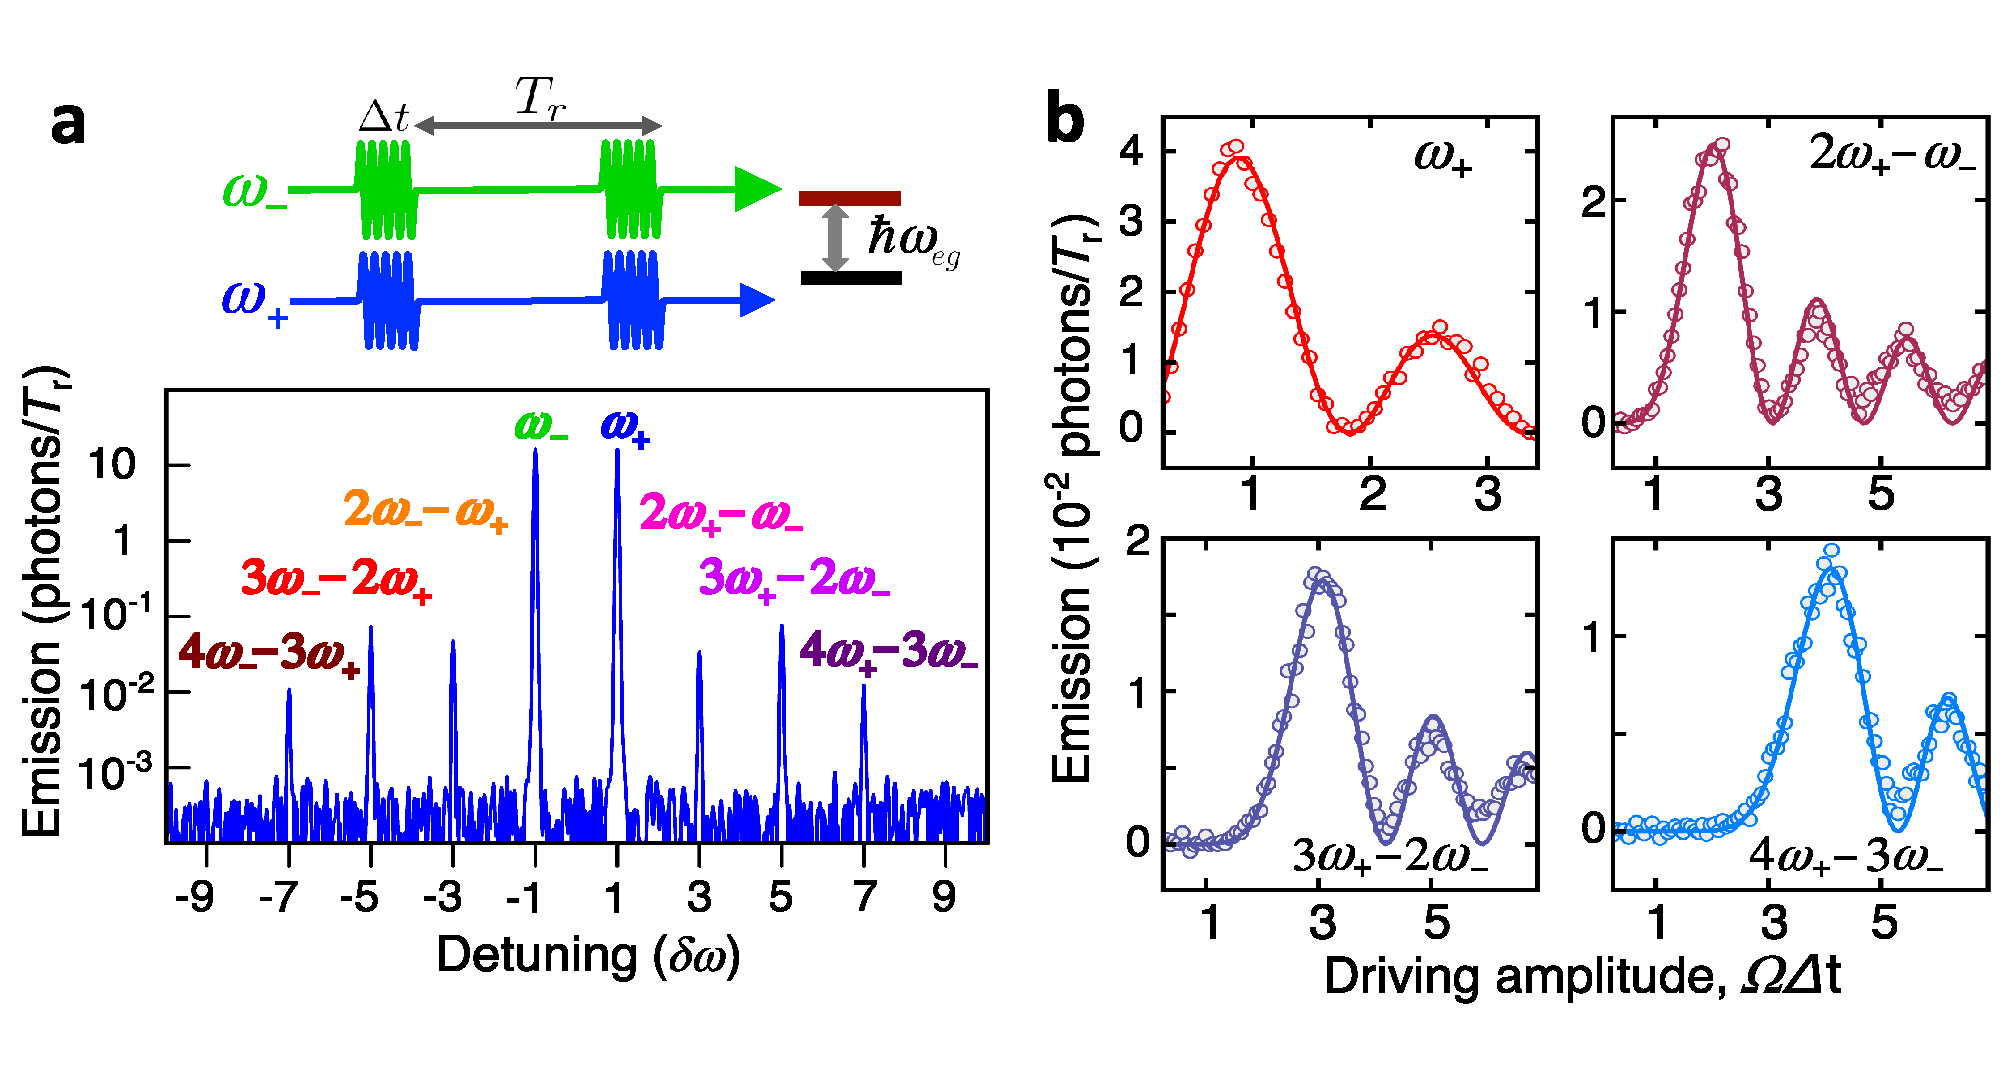
\includegraphics[width=1\textwidth]{Bessels.pdf}
\caption[Зависимость интенсивности боковых компонент от длительности импульсов $\Delta t$ бихроматической накачки]{Зависимость интенсивности боковых компонент от длительности импульсов бихроматической накачки. (a) Последовательность управляющих импульсов длительностью $\Delta t=2$~нс с периодом $T_r=1$~мкс и часть спектра эластичного рассеяния c когерентыми пиками. (б) Измеренные зависимости потока фотонов в пике от угла поворота $\zeta_{2p+1}(\Omega \Delta t). $. Точками показаны результаты измерений, сплошные линии соответствуют выражениям $J^2_{2p+1}(2\Omega\Delta t)/4$, описывающим эксперимент без подгоночных параметров.}
\end{figure} 
Этот результат достаточно просто объясняется динамикой кубита под воздействием классического поля. Для динамики кубита под действием двух классических импульсов можно получить следующее выражение:
\begin{equation}
	\braket{\sigma_-} = -\frac{1}{2}\sin(2\Omega\Delta t \cos\delta\omega t), 
\end{equation}
которое раскладывается в ряд по бесселевским функциям согласно соотношению Ангера-Якоби:
\begin{equation}
	\langle \sigma^- \rangle = -\sum_{k=-\infty}^\infty (-1)^k J_{2k+1}(2\Omega \Delta t) \cos[(2k+1)\delta\omega t],
\end{equation}
и усреднение спектральных компонент $\langle \sigma^-_{2k+1}\rangle$ с определенным набегом фазы $(2k+1)\delta \omega t$ дает:
\begin{equation}
	\langle \sigma_{2k+1}^-\rangle = \frac{(-1)^k}{2}J_{2k+1}(2\Omega t),
	\label{sclass_spectr} 
\end{equation} 
что соответствует экспериментально представленным зависимостям на Рис.~\ref{fig: Bessels}. Данный результат можно представить как разложение осцилляций Раби, которые наблюдались бы при $\delta\omega =0$, по разным спектральным компонентам.

Вывод результата \eqref{sclass_spectr} достаточно прост и не требует квантовомеханического описания поля, но тем не менее, он не иллюстрирует сущность наблюдаемого волнового смешения, в частности, не выделяет индивидуальный вклад различных многофотонных процессов в излучение и связь с фотонной статистикой излучаемого света. Более того, полуклассическая картина не выявляет физического происхождения ограниченного количества спектральных компонент, которые мы будем наблюдать для случая квантового волнового смешения двух последовательностей импульсов бихроматической накачки с задержкой. Поэтому мы получим бесселевскую динамику также при помощи рассмотрения эволюции кубита под воздействием двух квантованных мод поля, описывающихся операторами $a_\pm$ и $a_\pm^\dag$, взаимодействующих с кубитом. Как мы увидим далее, этот формализм позволяет описать не только случай синхронных импульсов, характеризующийся рассмотренной выше бесселевской динамикой, но и случай последовательных неперекрывающихся во времени импульсов, где спектр кардинально отличается от рассмотренного выше режима. Для начала, выпишем и обсудим несколько известных результатов, касающихся взаимодействия для одной моды внутри волновода и кубита, связанного с этим волноводомё. 

Будем рассматривать двухуровневый атом с основным и возбужденными состояниями $\ket{g}$ и $\ket{e}$ и энергией $\hbar \omega_0$, взаимодействующий с квантованным полем на частоте $\omega$. Эта система может характеризоваться гамильтонианом, записанным в представлении взаимодействия:
\begin{equation}
	H = i\hbar g (a^\dag \sigma^-  e^{i\delta\omega t} - a \sigma^+  e^{-i\delta\omega t}),
	\label{Hqint}
\end{equation}
где $\hbar g$ --- энергия связи между полем и атомом, $\delta\omega = \omega - \omega_0$ --- отстройка, которую мы считаем достаточно малой, $\sigma^{+} = \ket{e}\bra{g}$ и $\sigma^{-} = \ket{g} \bra{e}$ --- повышающий и понижающий операторы для состояний атома, а $a^\dag$ ($a$) --- операторы рождения и уничтожения фотонных состояний $|n\rangle$  на частоте $\omega = \omega_0 + \delta\omega$. 
Эволюция системы на коротком временном интервале $\Delta t \ll \delta\omega^{-1}$ описывается оператором $U(t',t) = \exp(-\frac{i}{\hbar} H_t \Delta t)$, где $H_t$ --- гамильтониан в момент времени $t$, $\Delta t = t'-t$. Оператор эволюции может быть разложен в бесконечный ряд по формуле:
\begin{equation}
	\begin{split}
		U(t',t) = 1 + 
		\eta (a^\dag s^- - a s^+ ) 
		-\frac{\eta^2}{2!} (a a^{\dag} s_{e} + a^{\dag}a s_{g} ) -
		\frac{\eta^3}{3!} (a^{\dag} a a^\dag s^- - a a^{\dag}a s^+)+... ,
	\end{split}
	\label{ut}
\end{equation}
где $\eta = g\Delta t$ и $s^\pm$ --- зависящие от времени операторы $s^+(t) = \sigma^+ e^{-i\delta\omega t}$ и $s^-(t) = \sigma^- e^{i\delta\omega t}$. 
Данный ряд можно записать в более простом виде: 
\begin{equation}
	\begin{split}
	U(t',t) =  \cos{\big(\eta \sqrt{a^\dag a}\big)} s_g &+ \cos{\big(\eta \sqrt{a a^\dag}\big)} s_e - \\
	&- \frac{a s^+}{\sqrt{a^\dag a}} \sin{\big(\eta \sqrt{a^\dag a}\big)} + \frac{a^\dag s^-}{\sqrt{a a^\dag}} \sin{\big(\eta \sqrt{a a^\dag}\big)},
	\end{split}	
\end{equation}
где $s_e = s^+ s^-$ and $s_g = s^- s^+$. Преобразуя далее, имеем:
\begin{equation}
	\begin{split}
		U(t',t) = \sum_{n=0}^{\infty} \Big[  \cos{\big(\eta \sqrt{n}\big)} &|n\rangle\langle n| s_g + \cos{\big(\eta \sqrt{n+1}\big)} |n\rangle\langle n| s_e - \\ 
		&|n\rangle\langle n+1| s^+ \sin{\big(\eta \sqrt{n}\big)} + |n+1\rangle\langle n| s^- \sin{\big(\eta \sqrt{n+1}\big)} \Big].	
	\end{split}
	\label{ut}
\end{equation}
В частности, для начального состояния $\Psi(t) = \ket{g,n}$, эволюция в результате приводит к состоянию $\Psi(t')=\cos(\eta \sqrt{n}) \ket{g,n}-e^{-i\delta\omega t} \sin(\eta \sqrt{n}) \ket{e, n-1}$. Мы будем рассматривать эволюцию под воздействием сильного когерентного излучения  $\ket{\alpha}$, где действительное $\alpha \gg 1$.

Когда $\Psi(t) = |g,\alpha\rangle$, эволюция упрощается:  
\begin{equation}
	\Psi(t') \approx \cos\frac{\theta}{2} \ket{g, \alpha} - e^{-i\delta\omega t} \sin \frac{\theta}{2} \ket{e, \alpha}
	\label{Rb}
\end{equation}
где $\theta = 2\eta\alpha$, $\alpha = \sqrt{\langle n\rangle}$ и $|\alpha'\rangle = \Big(1-e^{-|\alpha |^2}\Big)^{-1/2}\sum_{n=1}^\infty |n-1\rangle\langle n|\alpha\rangle $. В интересующем нас случае $\alpha \gg 1$ и поэтому поглощение одного фотона атомом эффективно не меняет состояние: $\ket{\alpha'} \approx \ket{\alpha}$. Мы можем переписать состояние в \eqref{Rb} как: 
$\Psi(t') \approx (\cos\frac{\theta}{2} |g\rangle - e^{-i\delta\omega t}\sin \frac{\theta}{2} |e\rangle)\otimes |\alpha\rangle$. После прохождения импульса, фотонное поле полностью излучается ($|\alpha\rangle \rightarrow |0\rangle$) и состояние системы приобретает вид:   
\begin{equation}
	\begin{split}
		\Psi' = \bigg(\cos\frac{\theta}{2} |g\rangle - e^{-i\delta\omega t}\sin \frac{\theta}{2} |e\rangle\bigg)\otimes |0\rangle 	
	\end{split}
	\label{Rb2}
\end{equation}
и для среднего значения оператора понижения с учетом фазы имеем:
\begin{equation}
	\langle s^+ \rangle = -\frac{\sin{\theta}}{2}.
	\label{sp}
\end{equation}

Атом, находящийся в состоянии суперпозиции (при $\theta \neq M \pi$, где $M$ это целое число) приобретает фазу $\delta\omega t$ из начальной когерентной волны \cite{Astafiev2010resonance,abdumalikov2011dynamics} и затем излучает в волновод суперпозицию нуля и одного фотона. 
%This can be exemplified by analysing the evolution $U(t')\Psi' = (\cos\frac{\theta}{2} |g, 0\rangle - ie^{i\phi}(\sin\frac{\theta}{2}\cos\frac{\theta'}{2} |e, 0\rangle - i\sin\frac{\theta}{2}\sin\frac{\theta'}{2} |g, 1\rangle)$, where $\theta' = 4 g t'$. 
Полезно проанализировать эволюцию состояния $\Psi'$ из уравнения \eqref{Rb2} под действием оператора (\ref{ut}). Когда накопленный угол $\eta = \frac{\pi}{2}$, % $U_{ap} = 1-i (s^- a^\dag+s^+ a)$ 
\begin{equation}
	U_{ap} = |0\rangle\langle0| \sigma^-\sigma^+ + e^{i\delta\omega t} |1\rangle\langle 0 | \sigma^-
	\label{Uap}
\end{equation} 
и суперпозиция атомного состояния перетекает в суперпозицию однофотонного поля на частоте $\omega$ следующим образом:    
\begin{equation}
	%\begin{split}
	U_{ap} \bigg[ \bigg(\cos{\frac{\theta}{2}} |g\rangle - e^{-i\delta\omega t} \sin{\frac{\theta}{2}} |e\rangle\bigg) \otimes |0\rangle \bigg] =  
	|g\rangle \otimes \bigg(\cos{\frac{\theta}{2}} |0\rangle - \sin{\frac{\theta}{2}} |1\rangle\bigg).
	\label{sps}
\end{equation} 
Мы введем однофотонный оператор рождения $b^+ = |1\rangle\langle0|$  на частоте $\omega$ и тогда
\begin{equation}
	\langle b^+\rangle = -\frac{1}{2}\sin\theta. 
	\label{bp}
\end{equation}
Уравнения (\ref{sp} - \ref{bp}) теперь могут быть переписаны при помощи $b$-операторов и важным следствием этого является тот факт, что состояние суперпозиции в атоме переходит в когерентное однофотонное поле при замене $s^+ \rightarrow b^+$ и $s^- \rightarrow b^-$, где введен оператор $b^- = |0\rangle\langle 1|$. 

%Importantly, the generated field is coherent, however essentially different from the classical coherent state $|\alpha \rangle=e^{-{|\alpha|^2}/{2}}\sum_{n=0}^{\infty}\alpha^n /\sqrt{n!} |n\rangle$ and $\alpha = \sqrt{\langle n\rangle}$ consisting of an infinite number of photon states. 

Классическое когерентное и однофотонное состояния могут быть представлены в похожей форме: 
\begin{subequations}
	\begin{alignat}{2}
		|&\alpha\rangle = & A \bigg( & |0\rangle + \alpha |1\rangle + \frac{\alpha^2}{\sqrt{2!}} + ...\bigg)\\
		|&\beta\rangle = & B \big( & |0\rangle + \beta |1\rangle\big),
	\end{alignat}
\end{subequations}
где $A=\exp{(-|\alpha|^2/2)}$ и $B=(1+|\beta|^2)^{-1/2}$. В частности, для когерентного состояния из уравнения \eqref{sps}, $\beta = -\tan \theta/2$ и $B=\cos \theta/2$. 

На основе вышеизложенного, гамильтониан~\eqref{Hqint} может быть эквивалентным образом представлен при помощи однофотонных операторов рождения и уничтожения следующим образом: 
\begin{equation}
	H' = i\hbar g (b^+ a - b^- a^\dag),
	\label{Hqintb}
\end{equation}
подразумевая, что $b$-операторы описывают фотоны, излученные атомом с фазой $\delta\omega t$ и потому удовлетворяют соотношениям, типичным для $s$-операторов: $b^+b^- = |1\rangle\langle 1|$, $b^-b^+ = |0\rangle\langle 0|$, $b^+b^+ = 0$, $b^-b^- = 0$. 

В дополнение, можно упростить уравнение~(\ref{ut}) для случая достаточно коротких импульсов достаточно сильного когерентного поля следующим образом: 
%\begin{equation}
%\begin{split}
%	U(t',t) = \sum_{n=0}^{\infty} &\cos{\big(\eta \sqrt{n}\big)} |n\rangle\langle n| b^-b^+ + \cos{\big(\eta \sqrt{n+1}\big)} |n\rangle\langle n| b^+b^- -\\ 
%	&\sin{\big(\eta \sqrt{n}\big)} |n-1\rangle\langle n| b^+ + \sin{\big(\eta \sqrt{n+1}\big)} |n+1\rangle\langle n| b^-.	
%\end{split}
%\label{ut}
%\end{equation}
%
%\begin{equation}
%	U(t',t) = \cos{\big(\eta \sqrt{a^\dag a}\big)} b^-b^+ + \cos{\big(\eta \sqrt{a a^\dag}\big)} b^+b^- -
%	\frac{a b^+}{\sqrt{a^\dag a}} \sin{\big(\eta \sqrt{a^\dag a}\big)} + \frac{a^\dag b^-}{\sqrt{a a^\dag}} \sin{\big(\eta \sqrt{a a^\dag}\big)}.	
%\end{equation}
%
\begin{equation}
	U(t',t) \approx \cos{\big(\eta \sqrt{a^\dag a}\big)} + (a^\dag b^- - a b^+) \frac{\sin{\big(\eta \sqrt{a^\dag a}\big)}}{\sqrt{a^\dag a}}.	
	\label{u1}
\end{equation}

%\begin{equation}
%\langle b^+_{2k+1} \rangle = \frac{(-1)^k}{2}  J_{2k+1}[2\Omega\Delta t]. 
%\end{equation}

Вернемся к случаю импульсной бихроматической накачки. Для этого, мы рассматриваем два непрерывных когерентых поля $|\alpha_{-}\rangle_-$ и $|\alpha_{+}\rangle_+$, где $\alpha_{\pm}$ --- действительные комплексные амплитуды поля. Гамильтониан \eqref{Hqintb} принимает вид:
\begin{equation}
	%H = \hbar g \sum\limits_{k=0}^{\infty} (\sigma^+ a_{\pm(2k+1)} + \sigma^- a^\dag_{\pm(2k+1)}),
	%H = \hbar g (\sigma^+ a_{1} + \sigma^+ a_{-1}+c.c.),
	%H = \hbar g (\sigma^+ a_{1} + \sigma^- a^\dag_{1} + \sigma^+ a_{-1} + \sigma^-a^\dag_{-1}),
	H_{2} = i\hbar g(s_-^-a^\dag_{-} - s_-^+ a_{-}  + s_+^- a^\dag_{+} + s_+^+ a_{+} ) ,
	\label{Hm}
\end{equation}
где $a^\dag_\pm$ ($a_\pm$) --- операторы рождения (уничтожения) фотона на частотах $\omega_\pm$, $s_+^\pm = \sigma e^{\mp i\delta\omega t}$, $s_-^\pm = \sigma e^{\pm i\delta\omega t}$ и $\hbar g$ обозначает константу связи кубита к модам. Оператор эволюции, соответствующий гамильтониану ~(\ref{Hm}) может быть расписан аналогично уравнению~(\ref{ut}), однако, каждое слагаемое содержит последовательные комбинации операторов $s_\pm^- a^\dag_{\pm}$ и $s_\pm^+ a_{\pm}$. Мы можем переписать гамильтониан через $b$-операторы при помощи подстановки $s_\pm^+ \rightarrow b_\pm^+$ and $s_\pm^- \rightarrow b_\pm^-$,  
\begin{equation}
	H = i \hbar g\big(b_-^+ a_{-}  - b_-^-a^\dag_{-} + b_+^+ a_{+} - b^-_+ a^\dag_{+} \big),
	\label{Hmb}
\end{equation}
где $b_\pm^\pm$ описывают возбуждение/релаксацию атома с фазой $\pm\delta\omega t$. Оператор эволюции $U(t',t) = \exp(-\frac{i}{\hbar} H_{t}\Delta t)$ может быть переписан в тензорной форме:  
\begin{equation}
	\begin{split}
		U =1 + \eta (b^-_m a^\dag_m - b^+_m a_m)  &- \frac{\eta^2}{2!}(b^+_m b^-_j a_m a^\dag_j + b^-_m b^+_j a_m^{\dag} a_j) + \\
		&+ \frac{\eta^3}{3!} (b^-_{m-j+p} a^\dag_m a_j a^\dag_p - b^+_{m-j+p} a_m a_j^{\dag} a_p) +...,
	\end{split}
	\label{ut2}
\end{equation}
где индексы принимают значения $\pm 1$. Мы опираемся на соотношения $b^+_m b^-_j b^+_p = b^+_{m-j+p}$ потому что $b$-операторы должны удовлетворять таким же соотношениям, как и $s$-операторы: $s_m^+ s_j^- s_p^+ = e^{-i m\delta\omega t}\sigma^+ e^{i j\delta\omega t}\sigma^- e^{-i p\delta\omega t}\sigma^+ = e^{-i (m-j+p)\delta\omega t}\sigma^+ = s_{m-j+p}^+$. Здесь мы расширили определения  $s$-операторов произвольной $l$-моды: $s_l^\pm = e^{\mp i l\delta\omega t} \sigma^\pm$. К примеру, это означает, что слагаемые третьего порядка $a_+ a^\dag_- a_+ b^+_3$ и $a_- a^\dag_+ a_- b^+_{-3}$ выражаются в создании однофотонных полей на частотах $\omega_{\pm 3} = \omega_0 \pm 3\delta\omega$. Обобщая, излучаемый свет может возникать на частотах $\omega_{\pm l}=\omega_0 \pm l\delta\omega$, где $l=2k+1,k = 0,1,2,..$. Среди всех членов в уравнении~(\ref{ut2}), дающих вклад в создание однофотонного поля на частотах $\omega_{\pm l}$, член низшего порядка состоит из $2k+2$ операторов: $2k+1$ $a$-операторов $a_\pm a^\dag_\mp a_\pm ... = (a_\pm a^\dag_\mp)^k a_\pm$ and один оператор $b_{\pm (2k+1)}^+$. 
%The lowest order term in Supplementary Eq.~(\ref{ut2}) resulting in creation of the single-photon field at frequency $\omega_0 \pm l\delta\omega$, where $l=2k+1$, consists of $2k+2$ operators: $2k+1$ $a$-operators $a_\pm a^\dag_\mp a_\pm ... = (a_\pm a^\dag_\mp)^k a_\pm$ and one $b_{\pm (2k+1)}^+$. %

Как было показано в работе \cite{Astafiev2010resonance}, атом в состоянии суперпозиции геренирует поле $V = \frac{\hbar\Gamma_1}{\mu}\langle s^-\rangle$. Обобщая это утверждение, мы можем записать выражение для однофотонного когеретного поля на частоте $\omega_{\pm (2k+1)}$:
\begin{equation}
	V_{\pm l} = \frac{\hbar\Gamma_1}{\mu}\langle b^-_{\pm (2k+1)}\rangle,
	\label{Vl}
\end{equation}
где $\mu$ --- дипольный момент перехода, в нашем случае зависящий от величины емкостной связи атома с волноводом. Мы делаем замену $s^- \rightarrow b^-_{\pm (2k+1)}$ потому что поле в $b$-моде может быть непосредственно измерено ВАЦ или любым другим АЦП.

%We start from an arbitrary single-photon state with two coherent fields $|\beta\rangle\otimes | \alpha_-\rangle\otimes |\alpha_+\rangle$ and the evolution of the single-photon field averaged out over the driving field degrees of fredom can be described as 
%\begin{equation}
%U_b(t,t') = \langle\alpha_-,\alpha_+| U(t,t') |\alpha_-\alpha_+\rangle. 
%\end{equation}
%We start from a atomic state (mapped on the single-photon field $|\beta\rangle$ as shown above) with two strong coherent driving fields with equal amplitudes $\Psi(t) = |\beta\rangle\otimes | \alpha\rangle_-\otimes |\alpha\rangle_+$, where $|\alpha| \gg 1$. 
Для того, чтобы проанализировать эволюцию, в качестве начального состояния выберем $\Psi(t) = |\beta\rangle\otimes | n\rangle_-\otimes |n\rangle_+$, где атом находится в суперпозиции, описываемой однофотонным когерентным состоянием  $|\beta\rangle$, а поле находится в состояниях $|n\rangle_\pm$ (где $n \gg 1$) с одинаковым числом фотонов в каждой моде.
Введем операторы:  
\begin{subequations}
	\begin{alignat}{2}
		\hat{A}_{2k}^{+-} = &\Bigg\{
		\begin{array}{lr}
			(a^\dag_- a_+)^{-k} & : k < 0\\
			(a^\dag_+ a_-)^k & : k \ge 0
		\end{array}
		&\quad
		\hat{A}_{2k+1}^- = &\Bigg\{
		\begin{array}{lr}
			(a_- a^\dag_+)^{-k} a_- & : k < 0\\
			(a_+ a^\dag_-)^k a_+ & : k \ge 0
		\end{array}
		\\
		\hat{A}_{2k}^{-+} = &\Bigg\{
		\begin{array}{lr}
			(a_- a^\dag_+)^{-k} & : k < 0\\
			(a_+ a^\dag_-)^k & : k \ge 0
		\end{array}
		&\quad
		\hat{A}_{2k+1}^+ = &\Bigg\{
		\begin{array}{lr}
			(a^\dag_- a_+)^{-k} a^\dag_- & : k < 0\\
			(a^\dag_+ a_-)^k a^\dag_+ & : k \ge 0 ,
		\end{array}
	\end{alignat}
\end{subequations}
которые удовлетворяют соотношениям $(\hat{A}^{+})_{2k+1}^\dag = \hat{A}^-_{2k+1}$, $(\hat{A}^{+-}_{2k})^\dag = \hat{A}^{+-}_{-2k}$, $(\hat{A}^{-+}_{2k})^\dag = \hat{A}^{-+}_{-2k}$. 
Оператор
\begin{equation}
	\hat{A}^-_{2k+1} b^+_{2k+1} 
	\label{Ap}
\end{equation}
создает единичный фотон на частоте $\omega_{2k+1}$ с минимально возможным числом фотонов, созданных или уничтоженных на частотах $\omega_\pm$.  
В частности, $A^-_{2k+1} |n_-,n_+\rangle = \big(\frac{(n_- + k)!}{n_-!} \frac{n_+!}{(n_+ - k-1)!} \big)^{\frac{1}{2}} |n_- + k, n_+ - k-1\rangle$, где $k>0$. В случае одинаковых и достаточно больших $n\gg 2k+1$, $A^-_{2k+1}|n,n\rangle \approx n^{k+\frac{1}{2}} |n + k, n - k-1\rangle$. 
Эволюция может быть упрощенно записана в следующей форме: 
\begin{equation}
	\begin{split}
	%U\Psi = \sum_{k=-\infty}^{\infty} \big[C^{+-}_{2k}\hat{A}_{2k}^{+-} b^-_0 b^+_{2k} + iC^{-}_{2k+1}\hat{A}_{2k+1}^{-} b^+_{2k+1} + C^{-+}_{2k}\hat{A}_{2k}^{-+} b^+_0 b^-_{2k} - iC^{+}_{2k+1}\hat{A}_{2k+1}^{+} b^-_{2k+1}\big] \Psi,
	U(t',t)\Psi(t) \approx \sum_{k=-\infty}^{\infty} \big[&\hat{A}_{2k}^{+-} C^{+-}_{2k} b^-_{k} b^+_{-k} + \hat{A}_{2k}^{-+} C^{-+}_{2k} b^+_{k} b^-_{-k} -\\- &\hat{A}_{2k+1}^{-} C^{-}_{2k+1} b^+_{2k+1} + \hat{A}_{2k+1}^{+} C^{+}_{2k+1} b^-_{2k+1}\big] \Psi(t),
	%U_b = \sum_{k=-\infty}^{\infty} \big[C_{2k}\langle\hat{A}_{2k}^{+-}\rangle b^-_0 b^+_{2k} + C_{2k+1}\langle\hat{A}_{2k+1}^{-}\rangle b^+_{2k+1} + C_{2k}\langle\hat{A}_{2k}^{-+}\rangle b^+_0 b^-_{2k} + C_{2k+1}\langle\hat{A}_{2k+1}^{+}\rangle b^-_{2k+1}\big]
	\end{split}
	\label{uc}
\end{equation}
где коэффициенты $C_l$ зависят от начального состояния и вычисляются как сумма по всем возможным перестановкам комбинаций из операторов рождения и уничтожения ($a^{~}_{-} a^\dag_{-}$, $a^\dag_{-} a^{~}_{-}$, $a^\dag_{+} a^{~}_+$, $a^{~}_{+} a^\dag_{+}$ для двух фотонов, вовлеченных в многофотонный процесс рассеяния, $a^{~}_+ a^{\dag}_- a^{~}_- a^{\dag}_+$, $ a_+^\dag a^{~}_- a_-^\dag a^{~}_+$ и два других члена для 4 фотонов, и т.д.), которые не меняют ни частоту,  ни заселенность фотонных состояний. Предполагая, что $n \gg 2k$ и принимая во внимание соотношения $a\ket{n}=n \ket{n}$, $a^\dag\ket{n}\approx n \ket{n}$, мы приходим к выражению: 
\begin{equation}
	%\frac{\eta^l}{l!}\times \frac{l!}{k! (l-k)!}
	%C_{l} = \frac{1}{\big(a_+^\dag a_+ \big)^{\frac{l}{2}}} \sum_{m=0}^\infty \frac{\bigg(i\eta\sqrt{a_+^\dag a_+}\bigg)^{l+2m}}{(l+2m)!} \frac{(l+2m)!}{m! (l+m)!} = \Bigg(\frac{i}{\sqrt{a^\dag_+ a_+}}\Bigg)^lJ_l \bigg(\eta \sqrt{a^\dag_+ a_+} t \bigg), 
	C_{l} \approx \frac{1}{(\sqrt{n})^l} \sum_{m=0}^\infty \frac{(-1)^{j+m}(\eta  \sqrt{n})^{l+2m}}{(l+2m)!} \frac{(l+2m)!}{m! (l+m)!} = \frac{(-1)^j}{(\sqrt{n})^l} J_l (\eta\sqrt{n}), 
\end{equation}
где $j = \mod(l,2)$, $J_l$ обозначают бесселевские функции первого рода. 

Если начальное состояние системы взять в виде $\Psi = |\beta,\alpha,\alpha\rangle$, где $\alpha$ действительно, то уравнение~(\ref{uc}) упрощается: 
\begin{equation}
	\begin{split}
	\sum_{k=-\infty}^{\infty} \bigg[&\frac{(-1)^k}{\alpha^{2k}}J_{2k}(\theta)\Big(\hat{A}_{2k}^{+-} b^-_{-k} b^+_{k} +\hat{A}_{2k}^{-+} b^+_{-k} b^-_{k} \Big) + \\
	&+ \frac{(-1)^k}{\alpha^{2k+1}}J_{2k+1}(\theta)\Big(\hat{A}_{2k+1}^{+} b^-_{2k+1} - \hat{A}_{2k+1}^{-} b^+_{2k+1}\Big)\bigg] \Psi
	\end{split}
\end{equation}
и для случая $\Psi = |0,\alpha,\alpha\rangle$:
\begin{equation}
	\begin{split}
	U\Psi \approx \sum_{k=-\infty}^{\infty} \bigg[&\frac{(-1)^k}{\alpha^{2k}}J_{2k}(\theta)\hat{A}_{2k}^{+-} |0\rangle_{2k} \otimes|\alpha,\alpha\rangle +\\
	&+ \frac{(-1)^k}{\alpha^{2k+1}}J_{2k+1}(\theta)\hat{A}_{2k+1}^{-} |1\rangle_{2k+1} \otimes|\alpha,\alpha\rangle \bigg], 
	\end{split}
\end{equation}
где $\theta = 2\eta\alpha$. 
%\begin{equation}
%U\Psi = \sum_{k=-\infty}^{\infty} \bigg[\frac{(-1)^k}{\alpha^{2k}}J_{2k}(\Omega t)\hat{A}_{2k}^{+-} e^{i2k\delta\omega t} b^-_{0} b^+_{2k}|0\rangle - \frac{(-1)^k}{\alpha^{2k+1}}J_{2k+1}(\Omega t)\hat{A}_{2k+1}^{-} b^+_{2k+1}|0\rangle \bigg] \Psi,
%\end{equation}
Принимая во внимание, что
$b^+_{2k+1} = |1\rangle_{2(k+p)+1}\langle 0|_{2p}$, мы можем напрямую записать выражение для квантовомеханического среднего оператора рождения фотона на частоте $\omega_{2k+1}$
\begin{equation}
	\langle b^-_{2k+1}\rangle =  \sum_{p=-\infty}^{\infty} \frac{(-1)^{k+p+p}}{\alpha^{2(k+p)+1}}J_{2(k+p)+1}(\theta)J_{2p}(\theta)\langle \hat{A}_{2(k+p)+1}^{-}\hat{A}_{-2p}^{+-}\rangle. 
\end{equation}
Используя стандартные соотношения для функций Бесселя, это выражение упрощается: 
\begin{equation}
	\langle b^-_{2k+1}\rangle = \frac{(-1)^kJ_{2k+1}(2\theta)}{2\alpha^{2k+1}}\langle\hat{A}_{2k+1}^{-}\rangle.
	\label{b22}
\end{equation}
Здесь было использовано следующее свойство: $\alpha^{-(2(k+p)+1)} \langle \hat{A}_{2(k+p)+1}^{-}\hat{A}_{-2p}^{+-} \rangle \approx\alpha^{-(2k+1)}\langle \hat{A}_{2k+1}^{-} \rangle$ for $\alpha \gg 1$.
Учитывая, что $\langle \hat{A}^-_{2k+1} \rangle \approx \alpha^{2k+1}$, мы упрощаем выражение:
\begin{equation}
	\langle b^+_{2k+1}\rangle = \frac{(-1)^k}{2} J_{2k+1}(2\Omega \Delta t),  
	\label{b2k1}
\end{equation}
где $\Omega \Delta t = \theta$. Окончательный ответ совпадает с  (\ref{sclass_spectr}).
Амлитуда когерентно рассеиваемого в каждую моду напряжения может быть записана как:  
\begin{equation}
	V_{2k+1} = \frac{\hbar \Gamma_1}{\mu}\langle b_{2k+1} \rangle, 
\end{equation}
что соотвествует мощности 
\begin{equation}
	W_{2k+1} = \frac{V^2_{2k+1}}{2Z_0} , 
\end{equation}
где $Z_0$ --- волновой импеданс. Теперь мы рассчитаем энергию когерентной волны за каждый цикл, подставляя уравнение~(\ref{b2k1}) в~(\ref{Vl}) и производя интегрирование по времени $t$. Учитывая, что $\Gamma_1 = \frac{\hbar\omega \mu^2 Z_0}{\hbar^2}$ и $\int_0^\infty \langle b_{2k+1} \rangle^2 dt = \int_0^\infty e^{-\Gamma_1t} = \Gamma_1^{-1}$, мы находим числа фотонов, излучаемых суммарно в две половины волновода:
\begin{equation}
	%V_{\pm(2k+1)} = \frac{\hbar\Gamma_1}{\mu}\frac{(-1)^{k+1}}{2}\times J_{\pm(2k+1)}(2\Omega \Delta t).
	\frac{E_{\pm(2k+1)}}{\hbar\omega} = \frac{J^2_{\pm(2k+1)}(2\Omega \Delta t)}{4}.
\end{equation} 

Несмотря на то, что аналитическое решение получено в приближении сильного драйва, его можно обобщить и на случай произвольных начальных состояний поля:
\begin{equation}
	\langle b^+_{2k+1}\rangle = D^-_{2k+1}\langle\hat{A}_{2k+1}^{-}\rangle,
	%\langle b^-_{2k+1}\rangle = B^-_{2k+1}\langle\hat{A}_{2k+1}^{+}\rangle. 
	\label{bg}
\end{equation}
где коэффициенты $D^-_{2k+1}$ зависят от амплитуд состояний поля. Точное аналитическое выражения для этих коэффициентов требует достаточно однообразных и рутинных вычислений, но не представляет значительного интереса и поэтому здесь не приводится. Также мы видим, что фотоны испускаются только на частотах $\omega_0 \pm (2k+1)\delta\omega$ с нечетными индексами $2k+1 > 0$. Создание такого однофотонного состояния требует уничтожения $k+1$ фотонов на частоте $\omega_+$ и создания $k$ фотонов на частоте $\omega_-$. 

В данном разделе мы теоретически и экспериментально рассмотрели бесселевский аналог осцилляций Раби, возникающий в рассеянном поле на боковых частотах при волновом смешении двух синхронных последовательностей импульсов на одиночном искусственном атоме. Теперь мы обратимся к эффекту, называемому квантовым волновым смешением, который проявляется в несимметрии эластичного спектра при рассеянии последовательности бихроматических импульсов с задержкой. Его необычность в том, что он может наблюдаться только при рассеянии на одиночном атоме, поэтому ранее он не был обнаружен в рамках традиционной квантовой оптики на ансамблях двухуровневых систем. 
\section{Введение задержки. Квантовое смешение волн}
\label{sec: qwm}
\begin{figure}
	\centering
	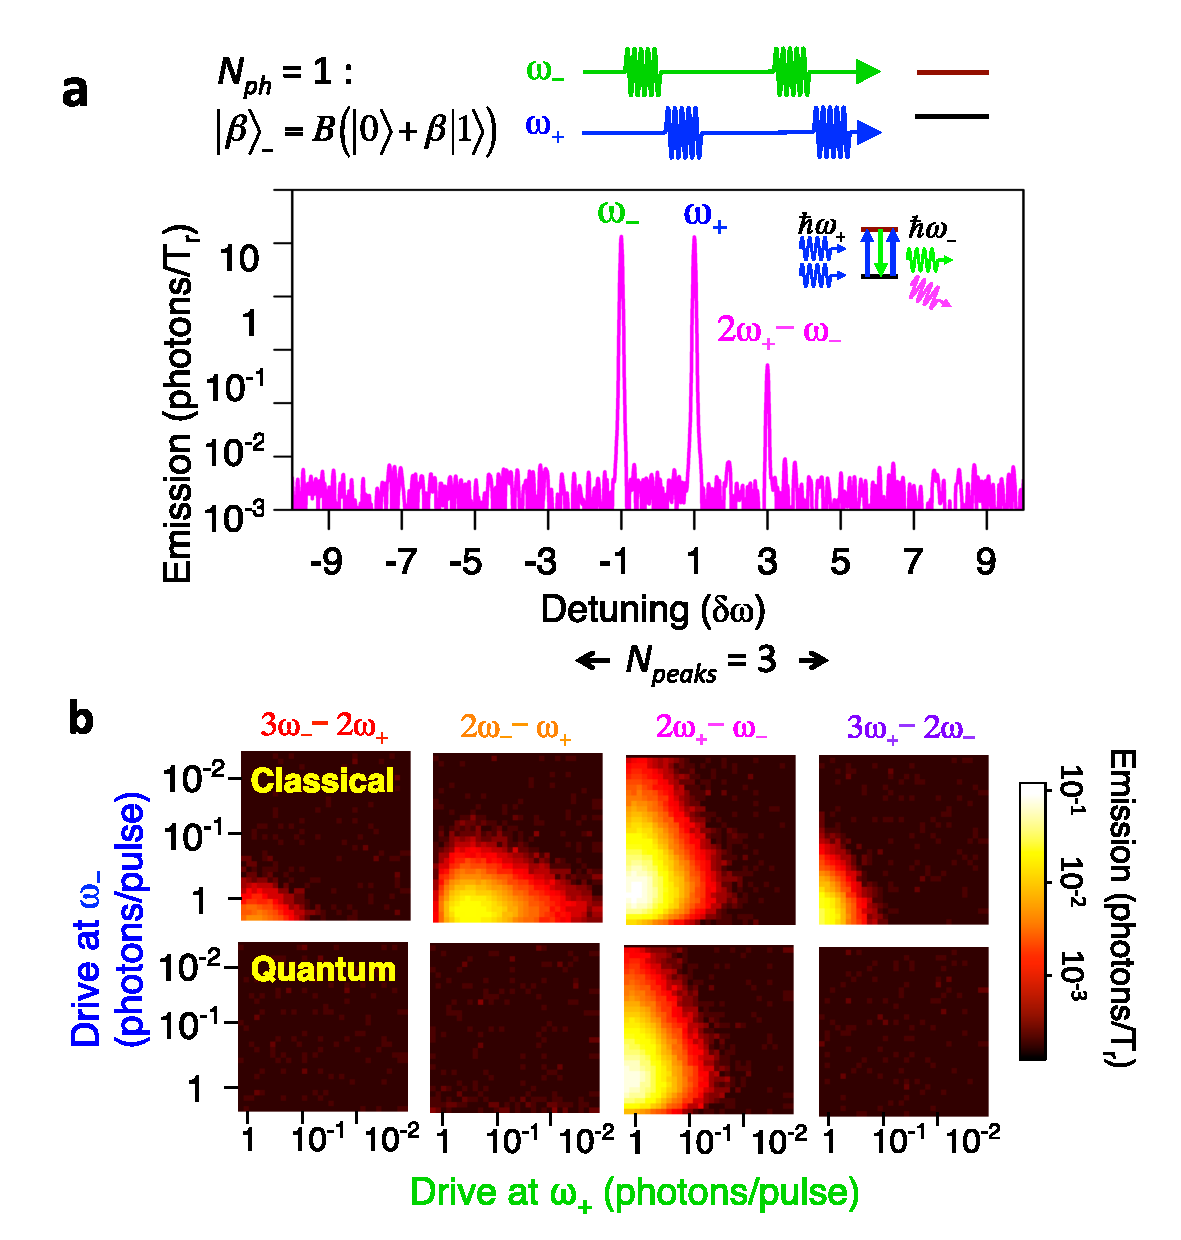
\includegraphics[width=0.8\textwidth]{Fig3_rev3.pdf}
	\caption[Квантовое волновое смешение неперекрывающихся импульсов: трехпиковый спектр.]{Квантовое волновое смешение неклассического света. (а) ---  Периодическая последовательность импульса на частоте $\omega_-$ и затем на частоте $\omega_+$ направляются на искусственный двухуровневый атом. График иллюстрирует спектр квантового волнового смешения от однофотонной когерентной суперпозиции $|\beta\rangle_-$. Единственный боковой пик возникает на частоте $2\omega_+ - \omega_-$ по причине комбинационного рассеяния фотона, $N_{ph} = 1$, от $|\beta\rangle_-$ и двух фотонов от когерентного поля второго импульса $|\alpha\rangle_+$. (b) -- Зависимость амплитуд боковых пиков при <<классическом>> смешении (в случае перекрывающихся импульсов) и квантовом смешении (случай последовательных импульсов) как функции амплитуд Раби  
		$\alpha_\pm$, выраженных в фотонах на цикл. Отчетливо наблюдается несколько боковых компонент в <<классическом>> режиме. Квантовый случай кардинально отличается полным отсутствием всех порядков, кроме пика на частоте $2\omega_+ - \omega_-$, который ведет себя практически так же как и в случае перекрывающихся импульсов. 
	}
	\label{fig: mixing_3peaks}
\end{figure}
Наблюдаемая нами в предыдущем разделе картина волнового смешения симметрична относительно частоты кубита, совпадающей с центральной частотой, причем это справедливо как для непрерывной, так и для импульсной накачки. Однако, в нашем распоряжении имеется еще один параметр, изменение которого может значительно повлиять на спектр эластичного рассеяния, изучаемый в данной работе. Этим параметром является задержка между импульсами различных частот. Можно предположить, что наиболее выразителен случай, когда задержка становится настолько большой, что первоначальные импульсы не перекрываются между собой во времени. Результат измерения эластичного спектра в этом случае приведен на Риc.~\ref{fig: mixing_mirror}а).

Введение задержки приводит к качественным изменениям в спектре: наблюдается единственная боковая спектральная компонента на частоте $\omega_{+3} = 2\omega_+-\omega_-$, если импульс на частоте $\omega_-$ предшествует импульсу на частоте $\omega_+$. Перестановка импульсов приводит к зеркально симметричному относительно центральной частоты (она же частота кубита) спектру, что опять же означает наличие единственной ненулевой боковой спектральной компоненты на частоте $\omega_{-3}$, см. Рис.~\ref{fig: mixing_mirror}. 
 
Одной из причин несимметричного спектра может являться большое различие в амплитуде полей $\Omega_+$ и $\Omega_-$, и ассимметрия может быть приписана смешению некоторого остаточного поля первого импульса со вторым импульсом. Чтобы доказать, что спектр содержит строго три пика и не больше, мы меняем амплитуды импульсов в широком диапазоне и измеряем интенсивности излучения на комбинационных частотах для случая классического и квантового смешения. Рис.~\ref{fig: mixing_3peaks}b) демонстрирует мощности излучения на боковых компонентах в различных режимах смешения: два перекрывающихся импульса\footnote{В данном разделе мы будем называть случай перекрывающихся импульсов классическим для того, чтоб отделять его от случая последовательных импульсов, где спектр более отличается от непрерывного поля. Однако, оба эффекта проявляются на квантовой двухуровневой системе и поэтому достаточно квантовые.} (верхние панели) и два последовательных импульса (нижние панели). Оба случая дают практически идентичную зависимость пика на частоте  $2\omega_+ - \omega_-$, однако остальные пики попросту отсутствуют в квантовом случае, появляясь только в классическом. 
\begin{figure}[th]
\centering
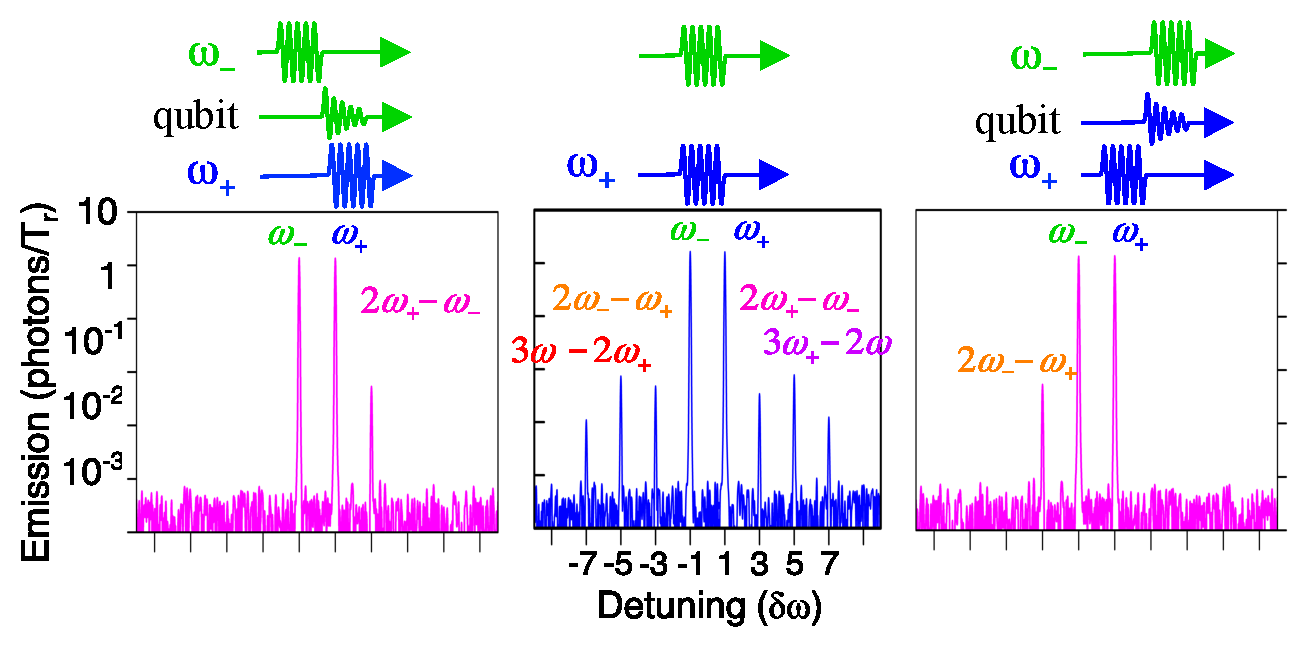
\includegraphics[width=0.9\textwidth]{QWM_slide_sqt.pdf}
\caption[Квантовое волновое смешение в зависимость от порядка импульсов]{Квантовое волновое смешение. Несимметричный трехпиковый спектр при перестановке импульсов претерпевает зеркальное отражение относительно центральной частоты. Центральный график соответствует случаю перекрывающихся импульсов, рассмотренному ранее. }
\label{fig: mixing_mirror}
\end{figure}

Наблюдаемый спектр может быть обоснован при помощи расчета оператора эволюции, подобно тому, как это было сделано в разделе \ref{sec: bessels}. Однако, прежде чем обратиться к точному теоретическому анализу наблюдаемого трехпикового спектра, полезно дополнительно подтвердить правильность предложенной качественной интерпретации. Напомним, что по нашему предположению, трехпиковый спектр объясняется тем, что двухуровневый атом <<запоминает>> единственное возбуждение, выделяя его из первого импульса, а затем происходит смешение этого возбуждения с полем из второго импульса, причем на единственно возможной частоте. Если аргументация верна, то крайне наглядно провести эксперимент по смешению на трехуровневой системе с уровнями $\ket{g}, \ket{e}, \ket{f}$, где разрешены переходы между соседними уровнями, и частоты этих переходов равны: $\omega_{ge} = \omega_{ef}$. Будем называть такую систему \textit{трехуровневой эквидистантной системой}. Очевидно, что она может запомнить два кванта возбуждения, и поэтому трехпиковый спектр должен модифицироваться в сторону увеличения числа наблюдаемых пиков. В следующем разделе мы покажем, что трехуровневую эквидистантную систему можно создать на основе того же самого потокового кубита, помещая его в определенную точку по магнитному потоку, а затем продемонстрируем как выглядит спектр квантового волнового смешения на трехуровневой эквидистантной системе. 
\section{Квантовое смешение волн на 3-уровневой системе}
Для того, чтобы определить возможность работы с потоковым кубитом в режиме квантовой трехуровневой эквидистантной системы, необходимо измерить спектр кубита в широком диапазоне. Результат измерения спектра приведен на Рис.~\ref{fig: flux_spectr_3ls}. Легко видеть, что для исследуемого потокового кубита имеется точка вблизи $\delta\Phi/\Phi_0 \approx  \pm 0.035$, где частоты переходов сравниваются, таким образом, система при ее взаимодействии с резонансной бихроматической накачкой эффективно становится трехуровневой. Направляя на кубит последовательность неперекрывающихся импульсов, рассмотренную в разделе~\ref{sec: qwm}, мы наблюдаем спектр волнового смешения, состоящий из пяти пиков, см. Рис.~\ref{fig: qwm_3ls}. 
\begin{figure}
	\centering
	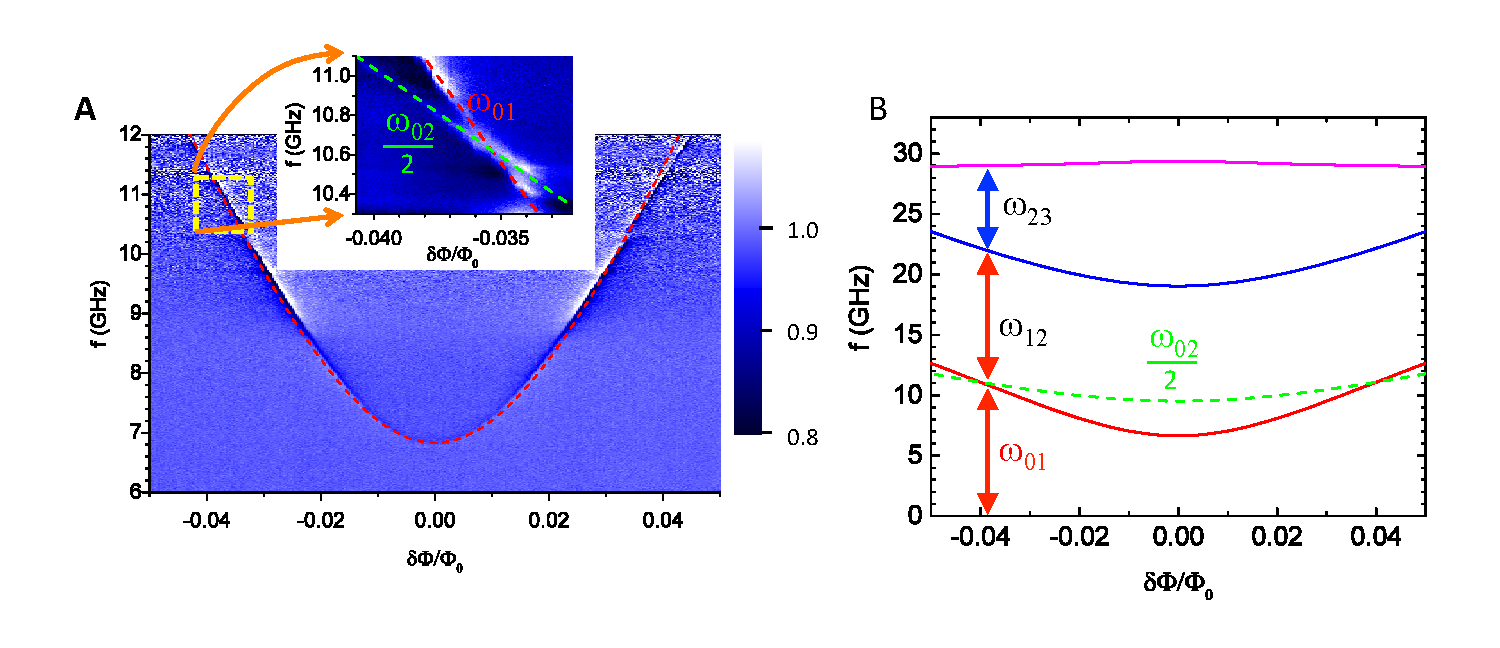
\includegraphics[width=1\textwidth]{SFig2.pdf}
	\caption[Спектр потокового кубита в широком диапазоне магнитного потока и нахождение рабочей точки, в которой кубит является трехуровневой эквидистантной системой.]{Измеренный (a) и рассчитанный (b) спектр потокового кубита в широком диапазоне магнитного потока и нахождение рабочей точки, в которой кубит является трехуровневой эквидистантной системой. Двухфотонный переход $\omega_{02}/2$ попадает в резонанс с переходом $\omega_{01}$. Отметим что за счет правил отбора в потоковом кубите в данной точке все три перехода являются разрешенными.}
	\label{fig: flux_spectr_3ls}
\end{figure}
\begin{figure}
	\centering
	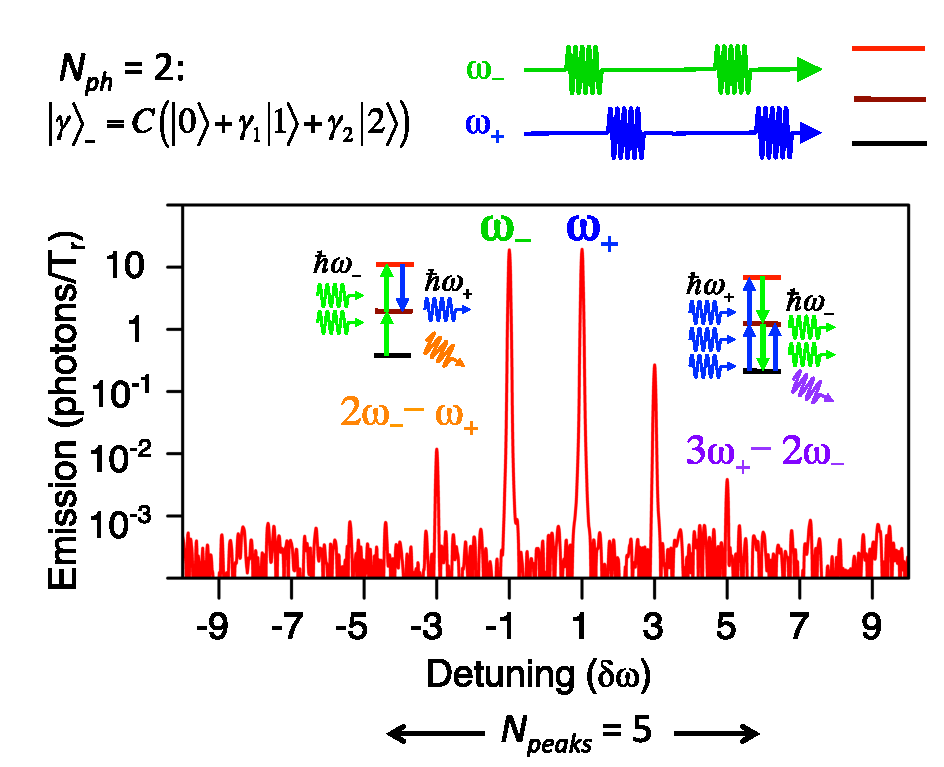
\includegraphics[width=0.6\textwidth]{Fig4_rev3.pdf}
	\caption[Спектр квантового волнового смешения на трехуровневой эквидистантной системе.]{Квантовое волновое смешение на трехуровневой эквидистантной системе с вовлечением двухфотонных состояний. Спектр смешения на трехуровневом атоме содержит три боковых пика, что является результатом отображения состояния системы с двумя возбуждениями $|\gamma\rangle_-$ ($N_{ph} = 2$). Сравнивая с Рис.~\ref{fig: mixing_3peaks}, дополнительный пик на частоте $3\omega_+ - 2\omega_-$ соответствуют двухфотонному излучению из состояния $|\gamma\rangle_-$. Процесс поглощения двух фотонов выражается в наличии пика на частоте $2\omega_- - 2\omega_+$, что завершает иллюстрацию всех разрешенных процессов при помощи спектра волнового смешения. Важно, что эксперимент отличает многофотонный случай на Рис.~\ref{fig: Bessels} ($N_{ph} = \infty$), однофотонное ($N_{ph} = 1$) и двухфотонное ($N_{ph} = 2$) состояния суперпозиции.}
	\label{fig: qwm_3ls}
\end{figure}
Поскольку вновь появившиеся пики возникли на частотах $\omega_{+5} = 3\omega_+-2\omega_-$ и $\omega_{-3} = 2\omega_--\omega_+$ --- на тех и только на тех частотах, которые вовлекают два фотона на частоте первоначального импульса $\omega_-$ --- то мы убеждаемся, что добавление третьего уровня и второго возбуждения в атом меняет картину смешения. Это является еще одним аргументом в пользу инерпретации спектра в качестве <<отпечатка>> различных многофотонных состояний, присутствующих в системе. Завершая обзор экспериментальных результатов в данной части диссертационной работы, приведем также сравнительную картину режимов волнового смешения в зависимости от угла поворота импульсов $\Omega\delta t$, см. Рис.~\ref{fig: qwm_all}. 
\begin{figure}
	\centering
	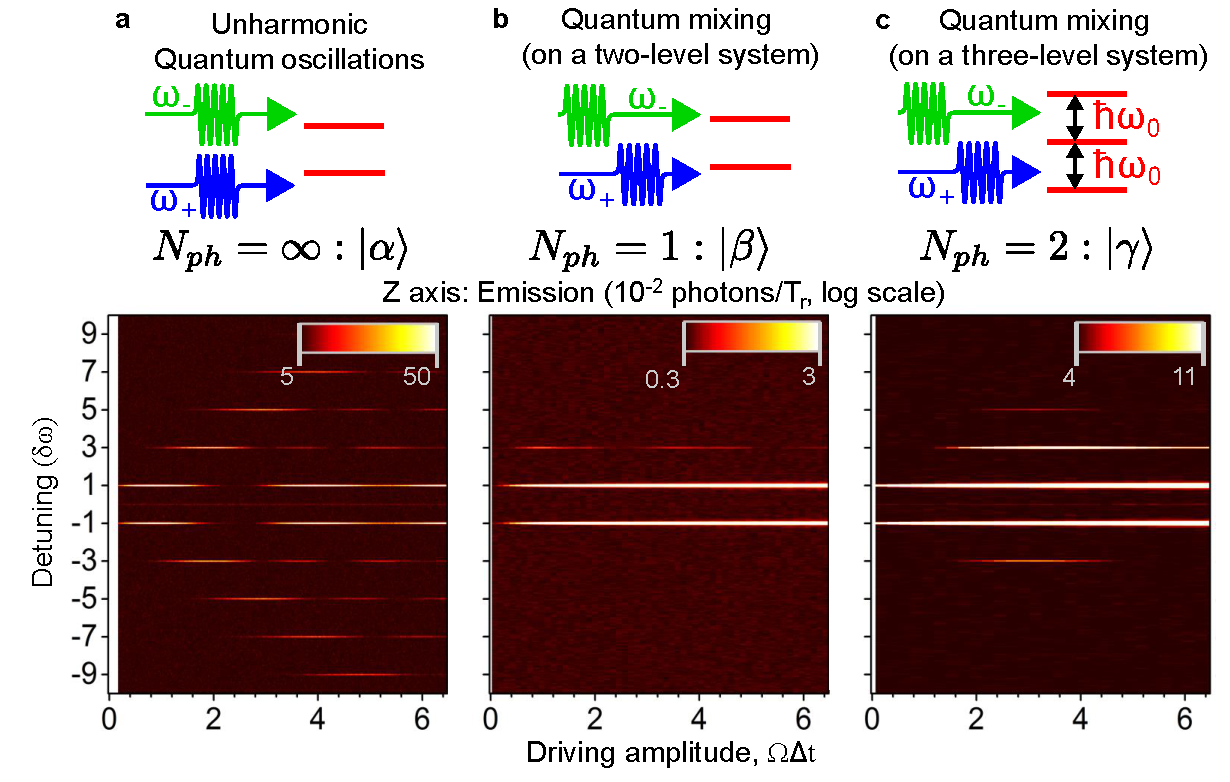
\includegraphics[width=0.9\textwidth]{Fig5_rev3.pdf}
	\caption[Сравнение различных режимов волнового смешения]{Различные режимы волнового смешения, представленные в виде зависимости от угла поворота импульсов. a) Бесселевское разложение осцилляций Раби в классическом волновом смешении на искусственном атоме. b) Квантовое волновое смешение на двухуровневой системе. Наблюдается одиночный боковой пик. c), Квантовое смешение на 3-уровневой системе. Два дополнительных боковых пика являются проявлением возможности возбуждения трехуровневой системы двумя фотонами, взятыми из начального импульса. }
	\label{fig: qwm_all}
\end{figure}
Мы установили, что спектр эластичного рассеяния при квантовом волновом смешении определяется свойствами как квантовой системы, на которой происходит смешение, так и временной диаграммой поля (говоря иначе --- конфигурацией возбуждающих бихроматических импульсов), распространяющегося в волноводе, где находится квантовая система. Для того, чтобы строго объяснить особенности спектров, проведем аналитический расчет интенсивности эластичных компонент поля. Это можно сделать на основе разобранного в разделе~\ref{sec: bessels} формализма. Аналитическому расчету интенсивности эластичных боковых компонент посвящается следующий раздел данной диссертационной работы.  
\section{Аналитический расчет спектров в представлении вторичного квантования}
Для того, чтобы получить спектр эластичного рассеяния для последовательностей неперекрывающихся импульсов, рассмотрим эволюцию под действием гамильтониана, записанного в представлении взаимодействия. Прожде всего отметим, что число мод в волноводе очень велико, но нас будет интересовать спектр от двух периодических сигналов, поэтому мы можем свести задачу к взаимодействию кубита поочередно с модами на частотах $\omega_-, \omega_+$. Поэтому достаточно использовать гамильтониан \eqref{Hqintb} и соответствующий ему оператор эволюции \eqref{u1}. 
\subsection{Случай двухуровневой системы}
Мы рассмотрим эволюцию под действием двух последовательных импульсов на частотах $\omega_-$ и $\omega_+$. Для удобства, мы возьмем начальное состояние в виде $\ket{0, \alpha_-, \alpha_+}$, но будем считать что операторы эволюции, определенные в уравнении~(\ref{u1}) действуют друг за другом в течении короткого времени. Иными словами, мы считаем что связь с каждой из мод включается только при прохождении соответствующего импульса через кубит. Для дальнейшего использования введем операторы:
\begin{equation}
\hat{\beta}^+_{\pm} = \beta_\pm a_\pm b^+_\pm (a^\dag_\pm a_\pm)^{-1/2}\approx \beta_{\pm}b^+_{\pm},
\label{beta_op}
\end{equation} 
где $\beta_\pm = \tan(\theta_\pm/2)$, $B_\pm = \sqrt{1+\beta_\pm^2}$, $\theta_- = 2g_- \alpha_- (t'-t)$, $\theta_+ = 2g_- \alpha_-(t''-t')$. Приближенное равенство в \eqref{beta_op} справедливо при условии $\alpha_{\pm} \gg 1$. С помощью этих операторов удобно записывать операторы эволюции. Первый импульс на частоте $\omega_-$ приводит к излучению поля в состоянии суперпозиции вакуума и одиночного фотона $|\beta\rangle_- = B_-(1-\hat{\beta}_-^+)\ket{0}$, что описывается эволюцией:
\begin{equation}
	U(t^\prime,t)\ket{0,\alpha_-,\alpha_+} =  B_- (1 - \beta_- b^+_-)\ket{0,\alpha_-,\alpha_+}=\ket{\beta_-}\otimes\ket{\alpha_-,\alpha_+},
\end{equation}
и это состояние мы обозначим $\ket{\beta_-,\alpha_-,\alpha_+}$. Затем это состояние эволюционирует при взаимодействии со вторым импульсом, представляемым когерентным состоянием $|\alpha\rangle_+$. Мы покажем, что среди всех процессов третьего или более высокого порядка, единственный нетривиальный вклад в среднее поле, приводящий к появлению излучения на новой частоте, дается слагаемым вида $A^-_{3} b^+_3 = a_- a^\dag_+ a_- b^-_3$, потому как всего один фотон может быть испущен на частоте $|\beta\rangle_-$. Все другие процессы оказываются запрещенными из-за того, что только одиночное возбуждение остается в кубите после взаимодействия с первым импульсом, что приводит к недостатку фотонов на частоте $\omega_-$. В итоге, единичный фотон может излучаться только на частоте $2\omega_+ - \omega_- = \omega_d + 3\delta\omega$. 

Эволюция под действием второго импульса записывается как 
\begin{equation}
	U(t',t'') |\beta_-,\alpha_-,\alpha_+\rangle \approx B_+ \bigg(1 + \hat{\beta}^-_+ - \hat{\beta}^+_+\bigg)  |\beta_-,\alpha_-,\alpha_+\rangle, 
	\label{Utt}
\end{equation}
Последнее равенство можно упростить: 
\begin{equation}
	U(t',t'') |\beta_-,\alpha_-,\alpha_+\rangle \approx B_+ B_- \Big(1 - \hat\beta^+_+  - \hat\beta^+_- - \hat\beta^-_+ \hat\beta^+_-\Big)|0,\alpha_-,\alpha_+\rangle, 
\end{equation}
также отметим что $\hat\beta^-_\pm =(\hat\beta^+_\pm)^\dag$. Как показано ранее, излучаемое поле на частоте $\omega_p$ пропорционально среднему от оператора уничтожения:
\begin{equation}
	\braket{b^-_p} = \braket{0,\alpha_-,\alpha_+|U^\dag(t',t)U^\dag(t'',t') b^-_p U(t'',t')U(t',t)|0, \alpha_-, \alpha_+}.
\end{equation}
Мы хотим сосчитать все фазовые факторы вида $e^{\pm i\delta\omega t}$, появляющиеся от операторов $\hat{\beta}^{\pm}_{\pm}$ и потом определить, для какого $p$ оператор $b^-_{p}$ усреднение по состоянию даст константу, не обращающуюся в ноль после усреднения по времени. Именно здесь и определятся частоты излучаемого поля в рамках когерентного рассеяния. После подстановки, мы получаем:
\begin{equation}
	\begin{split}
	\braket{b^-_p} = B_-^2B_+^2\bra{0,\alpha_-,\alpha_+}\big(
		&-\underbrace{b^-_p\hat{\beta}^+_+}_{e^{i\delta t}}
		-\underbrace{b^-_p\hat{\beta}^+_- }_{e^{-i\delta t}} \\
		&+\underbrace{\hat{\beta}^-_- \hat{\beta}^+_+ b^-_p  \hat{\beta}^+_-}_{e^{i\delta t}} 
		+\underbrace{\hat{\beta}^+_+ \hat{\beta}^-_-b^-_p\hat{\beta}^+_+  }_{e^{3i\delta t}}
		\big) \ket{0,\alpha_-,\alpha_+}
	\label{b_dag}
	\end{split}
\end{equation}
Мы видим, что среди всех членов \eqref{b_dag}, только последнее слагаемое создает поле на боковой частоте, потому как
\begin{equation}
	B_+^2 B_-^2\braket{\hat{\beta}^+_+ \hat{\beta}^-_-b^-_3\hat{\beta}^+_+ } = B_+^2 B_-^2\beta^2_+\beta_-\braket{\alpha_-,\alpha_+| \frac{A^-_{3}}{a^\dagger_+ a_+(a^\dagger_- a_-)^{1/2}}|\alpha_-,\alpha_+}
\end{equation}
отлично от нуля. 
Окончательно, среднее значение оператора находим как 
\begin{equation}
	\label{b3}
	\langle b^-_3 \rangle \approx B_+^2 B_-^2 \beta_+^2\beta_- = \frac{1}{2}\sin^2\left[\frac{\Omega_+}{2} (t''-t')\right]\sin\left[\Omega_- (t'-t)\right].
\end{equation}
Аналогичные выражения рассчитаны и для компонент на частотах $\omega_{-1}$ и $\omega_{+1}$. Также можно рассчитать аналогичные выражения для средних от операторов чисел заполнения в моде $\braket{b^+_p b_p}$, которые дают ненулевые значения на частотах $0, \pm 2 \delta\omega$. Зависимости для средних чисел заполнения не измерялись в эксперименте, но представляют важное дополнение к компонентам поля. Зависимости для среднего поля для компонент $\omega_{+3}, \omega_{+1}, \omega_{-1}$ и соответствующие зависимости чисел заполнения для частот $2\delta\omega, 0, \delta\omega$ приведены на Рис~\ref{fig: 2pulses}
\begin{figure}
\centering
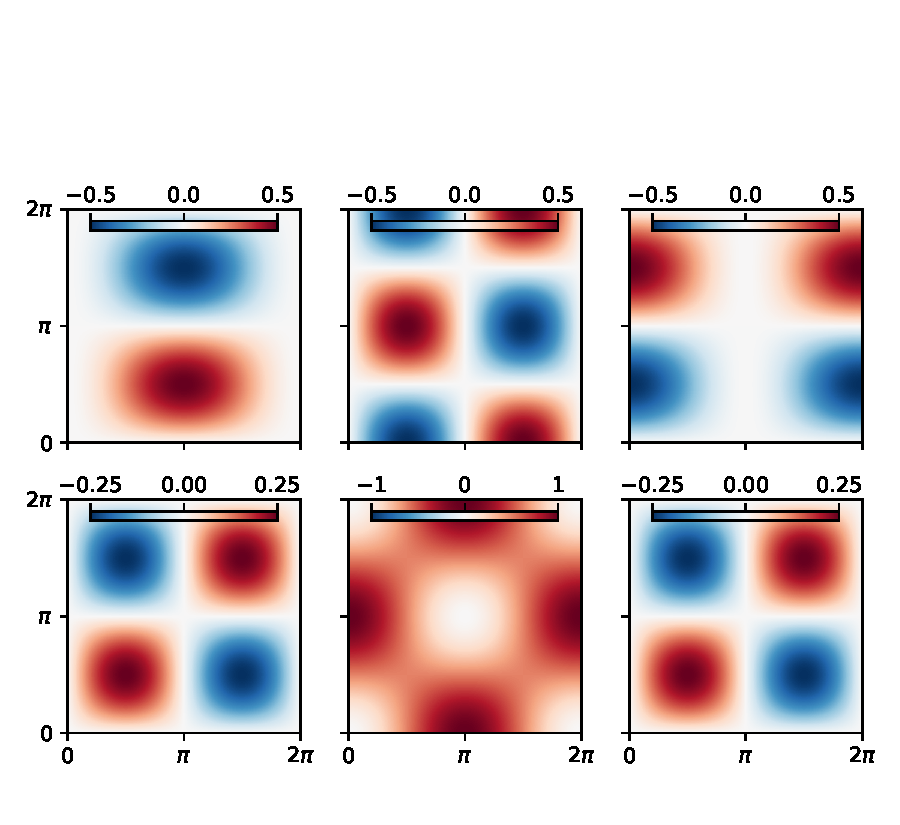
\includegraphics[width=0.7\textwidth]{2pulses_withZ.pdf}
\caption[Зависимости полей и средних заселенностей на боковых компонентах от углов поворота для квантового смешения]{Зависимость компонент поля (нижний ряд) на частотах (слева направо): $\omega_{+3}, \omega_{+1}, \omega_{-1}$, а также средней заселенности на частотах: $2\delta\omega, 0, -2\delta\omega$. Зависимости построены от углов поворота $\theta_-, \theta_+$. Левый верхний график соответствует выражению \eqref{b3}.   }
\label{fig: 2pulses}
\end{figure}

\subsection{Случай трехуровневой системы}
По аналогии с расчетом, представленным в предыдущем разделе, можно вычислить спектр смешения на эквидистантной трехуровневой системе. Уровни системы обозначим как $\ket{0}\!, \ket{1}\!, \ket{2}$. Предварительно отметим, что можно перейти к картине классического поля несколько раньше, а именно на этапе записи гамильтониана. Для начала мы считаем, что система испытывает воздействие со стороны резонансного монохроматического поля c эффективной амплитудой напряжения $V_0$. За счет диполь-дипольного взаимодействия это поле вызывает переходы $\ket{0}\rightleftarrows\ket{1}$ c частотой Раби:
\begin{equation}
\Omega_{01} = \mu_{01}V_0/\hbar \equiv \Omega.
\end{equation}
Это же монохроматическое поле вызывает также переходы $\ket{1} \rightleftarrows \ket{2}$, однако за счет другого дипольного момента (точнее, дипольного матричного элемента перехода) частота Раби будет отличаться: 
\begin{equation}
\Omega_{12} = \mu_{12}V_0/\hbar \equiv r\Omega.
\end{equation}
Параметр $r = \mu_{12}/\mu_{01}$ может быть точно рассчитан для конкретной схемы кубита посредством расчетов дипольных моментов для собственных состояний, полученных при помощи описанных в подразделе \label{subsec: flux_q} методик, а также определен экспериментально. В Главе 5 будет рассмотрен эксперимент по трехволновому смешению на потоковом кубите, работающем в режиме $\Delta$-системы. Рабочая точка по потоку в этом режиме несколько отличается от потока в режиме трехуровневой эквидистантной системы, но мы можем использовать данные работы \cite{PhysRevA.98.041801} и получить качественное представление о значении параметра $r$ можно при сравнении констант релакцации переходов, так как в общем случае $\Gamma_1 \propto \mu^2$. Из экспериментальных данных определено, что $\Gamma_1^{01}/2\pi = 8$~МГц и $\Gamma_1^{12}/2\pi = 38$~МГц, поэтому получаем:
\begin{equation}
r = \sqrt{\Gamma^{12}_1/\Gamma^{01}_1} \approx \sqrt{5}.
\end{equation} 
Гамильтониан во вращающейся системе запишем в виде:
\begin{equation}
H_3 = \left(
\begin{array}{ccc}
0 & \frac{1}{2} e^{i \phi } r \Omega  & 0 \\
\frac{1}{2} e^{-i \phi } r \Omega  & 0 & \frac{1}{2} e^{i \phi } \Omega  \\
0 & \frac{1}{2} e^{-i \phi } \Omega  & 0 \\
\end{array}
\right),
\end{equation}
и соответствующий ему оператор эволюции $U_\phi$ равен:
\begin{equation} 
 R^{-2}
 \left(
 \begin{array}{ccc}
 \left(R^2-1\right) \cos \frac{\theta }{2}+1 & -i R \sqrt{R^2-1} e^{i \phi } \sin \frac{\theta }{2} & \sqrt{R^2-1} e^{2 i \phi } \left(\cos
 \frac{\theta }{2}-1\right) \\
 -i R \sqrt{R^2-1} e^{-i \phi } \sin \frac{\theta }{2} & R^2 \cos \frac{\theta }{2} & -i R e^{i \phi } \sin \frac{\theta }{2}
 \\
 \sqrt{R^2-1} e^{-2 i \phi } \left(\cos \frac{\theta }{2}-1\right) & -i R e^{-i \phi } \sin \frac{\theta }{2} & \cos \frac{\theta
 }{2}+R^2-1 \\
 \end{array}
 \right),
 \label{U_3ls}
\end{equation}
где введены обозначения $R = \sqrt{r^2 + 1}$ и $\theta = R\Omega \Delta t$. При этом мы сохраняем фазу $\phi$  возбуждающего сигнала. Как мы увидим далее, именно фазовые множители, появляющиеся в \eqref{U_3ls}, накапливаясь по мере эволюции кубита под действием последовательных импульсов, порождают дополнительные спектральные компоненты.
По аналогии с \eqref{u1} мы можем записать полученный оператор в виде, визуализирующем процессы перехода.~Для этого введем операторы понижения в трехуровневой системе: $\hat{e} = \ket{0}\bra{1}\!,\:\hat{f} = \ket{1}\bra{2}$, которым соответствуют также операторы повышения $\hat{e}^\dag, \hat{f}^\dag$. Операторы рождения и уничтожения возбуждений в моде внешнего поля обозначим стандартно как $a^\dag, a$.
К примеру, для фиксированной фазы драйва $\phi = -\pi/2$ при помощи введенных оператор эволюции принимает вид:
\begin{equation}
	\begin{split}
	U = R^{-2}\Big[
	&\left(R^2+\cos \frac{\theta }{2}-1\right)\hat{e}\hat{e}^\dag + R^2 \cos \frac{\theta }{2} \hat{f}\hat{f}^\dag + \left(\left(R^2-1\right) \cos\frac{\theta }{2}+1\right) \hat{f}^\dag\hat{f} + \\
	+ &R \sin \frac{R \theta }{2} \left(a^\dag \hat{e}-a\hat{e}^\dag\right) + R \sqrt{R^2-1} \sin \frac{\theta }{2}\left(a^\dag \hat{f}-a\hat{f}^\dag\right) + \\
	+ &\sqrt{R^2-1} \left(\cos \frac{\theta }{2}-1\right)\left((a^\dagger)^2\hat{e}\hat{f} + a^2\hat{f}^\dag \hat{e}^\dag\right)
	\Big].
	\end{split}
\end{equation}
\begin{figure}[h]
	\centering
	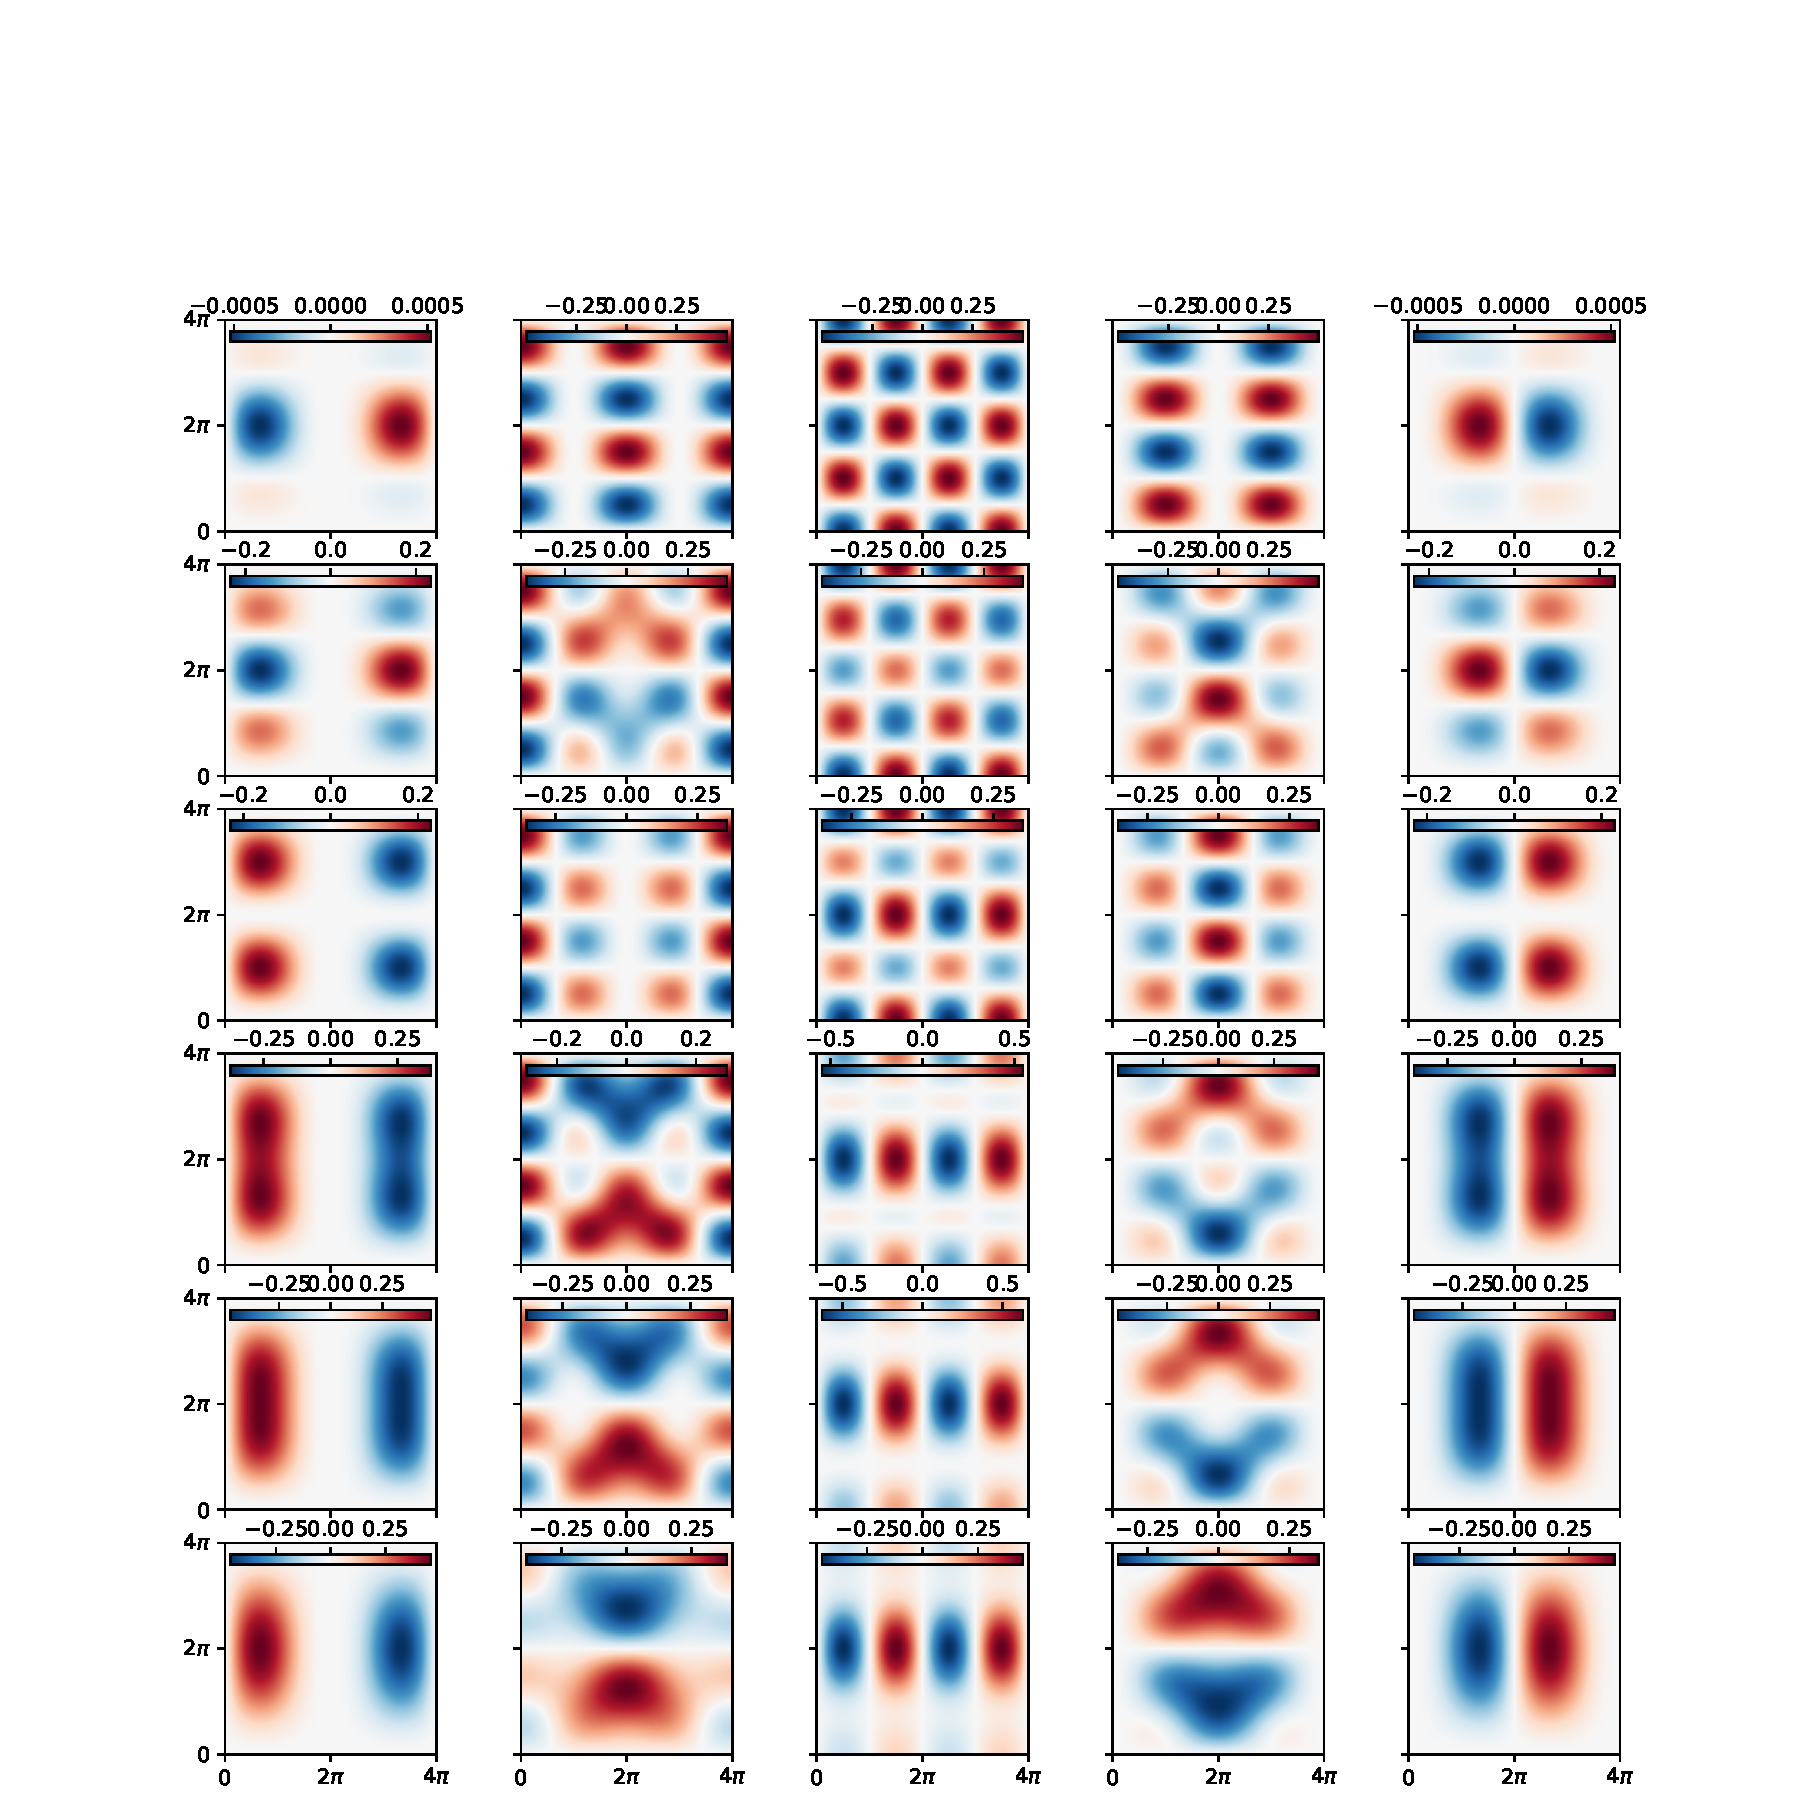
\includegraphics[width=1\textwidth]{3ls_mixing.pdf}
	\caption[Квантовое волновое смешение на трехуровневой эквидистантной системе] {Зависимости компонент волнового смешения на трехуровневой эквидистантной системе от $\theta_-, \theta_+$ для R = [1.0001, $\sqrt{1.5}$, $\sqrt{2}$, $\sqrt{3}$, 2, 5]. Постепенное <<включение>> перехода $\ket{1}\rightleftarrows\ket{2}$ значительно меняет характер зависимости от углов, в частности, делает зависимость 4$\pi$-периодичной. }
	\label{fig:maps_3ls}
\end{figure}
Отметим, что помимо однофотонных процессов, в системе возникли и двухфотонные переходы, где два кванта поля $a$ могут возбудить систему на уровень $\ket{2}$.
Нашей целью является расчет среднего поля в результате эволюции трехуровневой системы под действием двух последовательных импульсов на частотах $\omega_-, \omega_+$, который может быть записан как:
\begin{equation}
\braket{\hat{e} + r\hat{f}} = \bra{\psi_0}U^\dagger_-U^\dagger_+(\hat{e} + r\hat{f})U_+U_-\ket{\psi_0}.
\end{equation}
Здесь мы ввели операторы $U_-(\theta_-)$ и $U_+(\theta_+)$, которые получаются из оператора $U$ \eqref{U_3ls} при замене $\phi \rightarrow \phi_{\pm}, \Omega \rightarrow \Omega_{\pm}$. Начальное состояние $\ket{\psi_0} = \ket{0,\alpha_-, \alpha_+}$. Здесь можно продолжить расчет для представления вторичного квантования, но для полноты представляемой картины мы покажем, как получается результат для компонент смешения при классическом рассмотрении поля. Итак, напрямую перемножая матрицы, соответствующие операторам $U_-$ и $U_+$, и собирая члены с одинаковыми фазовыми множителями, получаем:
\begin{equation}
	\begin{split}
	\braket{\hat{e}+r\hat{f}} = i\Big[\Phi_- e^{i \phi _-} + \Phi_+ e^{i \phi _+} &+ \Phi_{+3}e^{i \left(2 \phi _+ -\phi_- \right)} +\\&+ \Phi_{-3}e^{i(2 \phi _-- \phi _+)} + \Phi_{+5}e^{i(3 \phi _+-2 \phi _-)}\Big],
	\end{split}
\end{equation}
где действительные функции $\Phi_{\cdot}(R, \theta_-, \theta_+)$ представляют зависимость компонент смешения от углов поворота импульсов. В явном виде они записываются достаточно громоздко, поэтому приведем графическое изображение этих функций от углов поворота при различных $R$, см. Рис.~\ref{fig:maps_3ls}. Верхний ряд картинок построен при $R=1.0001$, и этот случай практически полностью соответствует двухуровневой системе. Пики на частотах $\omega_-, \omega_+ \text{ и } \omega_{+3}$ показывают $2\pi$-периодичность по углам поворота. Однако, на всех других графиках поле, возбуждающее переход $\ket{1}\rightleftarrows\ket{2}$ не является пренебрежимо малым, и как следствие, возникает $4\pi$-периодичность компонент смешивания. Этот эффект требует дальнейшей теоретической интерпретации и экспериментального изучения, которые выходят за рамки данной работы. 

Как и для двухуровневой системы, спектр смешения в данном случае остается квантованным: имеется ровно 5 несимметрично расположенных пиков, что объясняется в рамках эволюции трехуровневой квантовой системы. Логично предположить, что и при дальнейшем увеличении количества уровней квантовой системы число пиков будет асимметрично увеличиваться до тех пор, пока картина не станет симметричной при бесконечном числе уровней, что будет соответствовать гармоническому осциллятору.
\section{Численный расчет импульсной динамики}
В завершение отметим, что приведенные зависимости достаточно прямолинейно получаются и при помощи численных расчетов. Например, с помощью пакета \verb|QuTiP| \cite{qutip1,qutip2} можно получить временную динамику как квантового состояния системы, так и любого среднего от произвольного оператора. Для этого мы задаем гамильтониан с зависящим от времени внешним полем, которое напрямую представляет из себя многопериодическую последовательность импульсов Раби. Добавляя коллапсирующие операторы релакcации, мы получаем численное решение основного квантового уравнения при помощи функции \verb|mesolve|. После взятия спектра мы получаем когерентные пики, соответствующие описанным выше эластичным компонентам, а также компоненты, соответствющие ненулевой средней заселенности мод. Поскольку эти результаты совпадают с аналитическими расчетами и не вносят дополнительной информации, описывающей вышеизложенные явления квантового волнового смешения, мы не приводим их в тексте данной диссертационной работы. 

После рассмотрения квантового волнового смешения на двухуровневой и трехуровневой эквидистантной системе, мы обращаемся к более сложному примеру искусственной квантовой системы на основе одиночного сверхпроводникового потокового кубита --- а именно, $\Delta$-системы с существенно различными частотами переходов. Такая система особенно сложнореализуема в рамках традиционной квантовой оптики, поскольку естественные правила отбора практически всегда запрещают дипольный переход между основным и вторым возбужденным энергетическими уровнями. В следующей главе будет описано, как происходит трехволновое смешение на $\Delta$-системе, и какими свойствами оно обладает. 


           % Глава 4
\chapter{Смешение волн на $\Delta$-системе}
Как упоминалось ранее, долгое время исследования в экспериментальной квантовой оптике были сосредоточены на изучении ансамблей природных, или естественных атомов \cite{Miller_2005,Walther_2006}. Однако, сверхпроводящие искусственные атомы крайне привлекательны для изучения явлений квантовой оптики. Их энергетические уровни могут быть спроектированы со значительным отличием от естественных атомов, и сильная связь с полем достигается не только в высокодобротных резонаторах \cite{wallraff2004strong}, но и в линих передачи (волноводах) \cite{Astafiev2010resonance, vanLoo1494}. Это позволяет воспроизводить явления квантовой оптики и даже достигать режимов, недоступных для естественных атомов. Интерес для применений представляют такие явления, как когерентный захват заселенности, электромагнитно-индуцированная прозрачность, расщепление Аутлера-Таунса --- многие из них были представлены в разделе \ref{sec: microwave qo}. В данной работе представлены также результаты по непрерывному волновому смешению (Глава \ref{ch: cwm}) и квантовому волновому смешению (Глава \ref{ch: q_mixing}), которые были впервые экспериментально изучены в сверхпроводящих искусственных атомах. Кроме того, сверхпроводящие трехуровневые системы могут быть использованы для охлаждения квантовых систем, усиления микроволновых сигналов и генерации одиночных или запутанных пар фотонов --- всего того, что является важным для создания квантовых сетей \cite{kimble2008quantum}.

В данной главе представлены результаты эксперимента по трехволновому квантовому смешению \cite{liu2014controllable}. Это нелинейный эффект, который может возникать в циклических трехуровневых атомах, фактически отсутствующих в природе, но легко реализуемых с помощью сверхпроводящих искусственных атомов. Единственными подходящими естественными системами для трехволнового смешения являются хиральные молекулярные трехуровневые системы без инверсионной симметрии \cite{PhysRevLett.111.023008}. Однако эти системы не могут быть перестраиваемыми по частоте. В отличие от параметрических трехволновых смесительных устройств на основе джозефсоновского перехода, которые полагаются на смешивание по классической нелинейности, мы реализуем здесь другой метод генерации трехволнового смешивания с использованием одного искусственного атома циклического типа, или $\Delta$-типа. Это явление теоретически рассмотрено в работах. Мы непосредственно измеряем когерентное излучение циклического трехуровневого атома при двух внешних резонансных возбуждающих сигналах, соответствующих двум атомным переходам \cite{PhysRevA.98.041801}. Излучение происходит на одной частоте --- сумме или разности частот драйва. Это излучение является следствием когерентного преобразования частоты, но по своей сути отличается от классического нелинейного преобразования частоты, которое привело бы к появлению боковых компонент на суммарной и разностной частотах. Ранее когерентные атомные возбуждения с использованием двух частот были исследованы при помощи фазового кубита, являющегося квантовой системой с двумя внутренними степенями свободы \cite{Lecocq2012}. Однако, состояние фазового кубита измерялось с помощью тока переключения, в то время как прямое детектирование когерентно преобразованного сигнала на циклическом искусственном атоме в открытом пространстве дает некоторые преимущества. В частности, можно непосредственно использовать когерентную (упругую) составляющую излучаемого поля на суммарной или разностной частоте переходов искусственного атома. Это открывает путь к инновационной квантовой электронике на основе трехволнового смешения или когерентного преобразования частоты.
\section{Режим $\Delta$-системы в потоковом кубите}
\begin{figure}
	\centering
	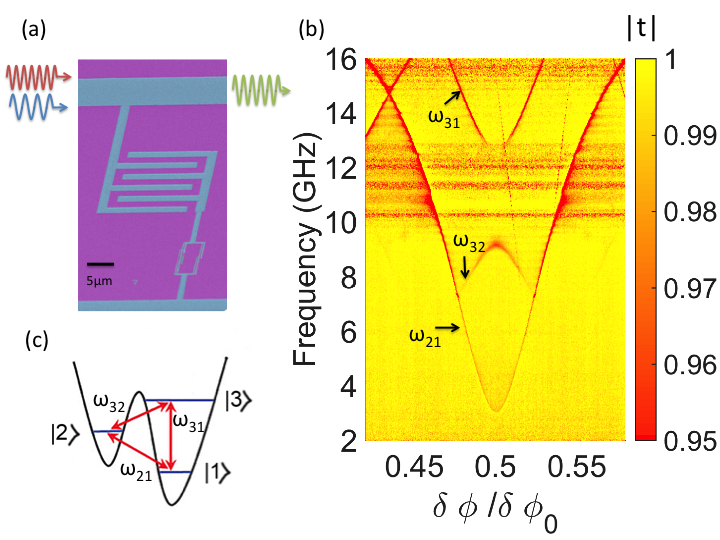
\includegraphics[width=0.8\textwidth]{figure1_Delta.png}
	\caption[Потоковый кубит в режиме $\Delta$-системы]{Сильно связанный с волноводом потоковый кубит, состоящий из 4 джозефсоновских переходов, электронное изображение которого представлено на панели (a), может находиться в режиме $\Delta$-системы при $\delta\phi \ne 0.5$. Однотоновая спектроскопия представлена на графике (b), верхние переходы становятся видимыми из-за большой мощности тона. (с), принципиальная схема переходов в циклическом атоме. Измерения проводятся при $\omega_{21}/2\pi = 6.48$ ГГц, $\omega_{32}/2\pi = 8.35$ ГГц, и $\omega_{31}/2\pi = 14.83$ ГГц.}
	\label{fig: flux_delta}
\end{figure}
Изучаемое устройство представляет собой потоковый кубит --- сверхпроводниковую петлю площадью около $\sim 10$~мкм$^{2}$, в которую вставлены четыре джозефсоновских перехода. Эта геометрия является модифицированной версией оригинального потокового кубита, предложенного в работе \cite{mooij1999josephson}, где один из трех переходов --- $\alpha$-переход --- имеет в $\alpha$ раз отличную площадь по сравнению с остальными переходами. Один из электродов получившейся петли связан с одномерным волноводом через встречно-штыревую емкость $C=6$~фФ, см. Рис.~\ref{fig: flux_delta}(a). Эта емкость определяет константу релаксации кубита в диапазоне от нескольких МГц до нескольких десятков МГц, в зависимости от частоты кубита. Основные параметры устройства --- джозефсоновская энергия $E_{J}/h=65$~ГГц, зарядовая энергия $E_{C}=e^2/2C$, $E_{C}/h=19$~ГГц и параметр $\alpha=0.45$ --- подобраны таким образом, чтобы все три частоты нижних переходов атома, см. Рис.~\ref{fig: flux_delta}c), попадали в допустимый частотный диапазон 2-18 ГГц нашего высокочастотного измерительного тракта. Скорость излучения в волновод для каждого из этих переходов достаточно велика для того, чтобы безызлучательная релаксация не играла значительной роли для наблюдаемых нами явлений. 

Точные значения частот переходов $\omega_{12}$, $\omega_{23}$, и $\omega_{13}$ контролируются при помощи внешнего магнитного потока, пронизывающего петлю кубита, $\Phi=\Phi_{0}/2+\delta\Phi$, где $\Phi_{0}$ --- квант магнитного потока и $\delta\Phi$ --- отстройка по потоку от точки симметрии, которая соответствует половине кванта магнитного потока. Частоты атомных переходов экспериментально определяются при помощи однотоновой спектроскопии на пропускание, измеряемой при помощи ВАЦ. Мы сканируем частоту пробного сигнала при различных значениях $\delta\Phi$, в результате получая спектр на Рис.~\ref{fig: flux_delta}b). Чтобы увидеть переход $|3\rangle \rightleftarrows |2\rangle$, необходимо значительно поднять мощность микроволнового тона, чтобы вызвать заметную заселенность уровня $\ket{2}$, который практически не заселяется в пределе слабой мощности. 
В рабочей точке по магнитному потоку частоты разрешенных переходов составляют $\omega_{21}/2\pi = 6.48$ ГГц, $\omega_{32}/2\pi = 8.35$ ГГц, и $\omega_{31}/2\pi = 14.83$ ГГц ($\omega_{31} = \omega_{21}+\omega_{32}$),  как схематично показано на Рис.~\ref{fig: flux_delta}(c). Отметим, что все три вышеперечисленные перехода разрешены только при ненулевой отстройке от $\delta\Phi = \Phi_0/2$, в то время как в точке симметрии переход $\ket{1}\rightleftarrows\ket{3}$ является запрещенным из соображений симметрии. Все измерения проводятся при базовой температуре криостата 12-15 мК, при которой тепловая заселенность пренебрежимо мала и не оказывает влияния на ход эксперимента.

\section{Описание эксперимента}
После завершения начальной характеризации образца, мы подаем на $\Delta$-систему два непрерывных сигнала, частоты которых практически совпадают с резонансными частотами каких-либо двух атомных переходов, и изучаем когерентное излучение системы на частоте третьего перехода, не возбуждаемого внешними сигналами. 
Измерения в каждом из показанных на Рис.~\ref{fig: 3wm_regimes} режимов проводились при различных значениях амплитуд Раби внешнего поля $\Omega_{ij}$ между состояниями $\ket{i}, \ket{j}$, где $i$ и $j$ принимают значения 1,2,3. Согласно квантовомеханическому описанию, излучение на боковой компоненте может возникнуть только в том случае, если она попадает в резонанс с каким-либо атомным переходом.

\begin{figure}[!th]
	\centering
	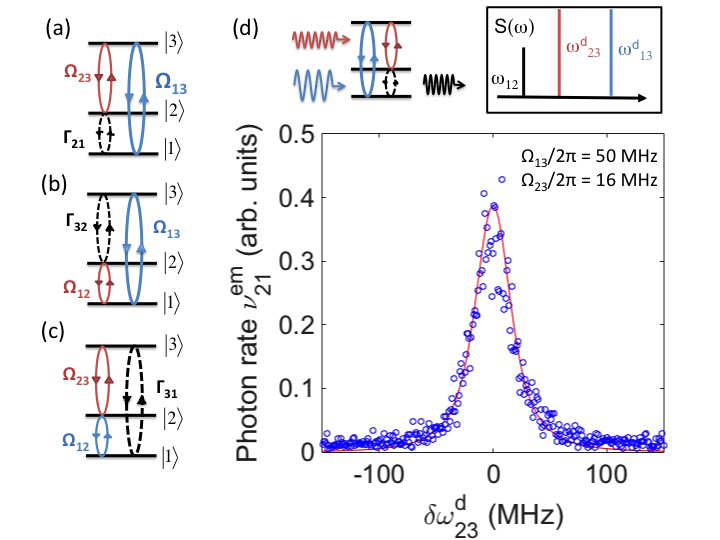
\includegraphics[width=0.8\textwidth]{figure2_Delta.png}
	\caption[Режимы трехволнового смешения на трехуровневой $\Delta$-системе]{Когерентное излучение на трехуровневой системе. Атом накачивается гармоническими сигналами на частотах: (a) $\omega_{23}$ и $\omega_{13}$; (b) $\omega_{12}$ и $\omega_{13}$; (c) $\omega_{12}$ и $\omega_{23}$. Амплитуды полей обозначены как $\Omega$ с индексами, соответствующими номерам уровней. (d) Мощность пика когерентного излучения на частоте $\omega_{12}$ в зависимости от отстройки $\delta\omega_{23}$, выраженная в единицах потока фотонов $\nu_{21}^{\text{em}}$. Атом находится под действием сигналов с амплитудами $\Omega_{23}/2\pi=16$ МГц, $\Omega_{13}/2\pi=50$ МГц. Вставка в правом верхнем углу схематично отражает полный спектр излучения $\Delta$-системы. }
	\label{fig: 3wm_regimes}
\end{figure}

Чтобы понять механизм происходящих физических процессов, можно обратиться к формализму вторичного квантования. При взаимодействия двух когерентных волн с одиночной квантовой системой, только один акт рассеяния (однофотонного или многофотонного) может происходить одномоментно, так как испущенное излучение улетает в волновод, и каскадные процессы становятся невозможными. Введем операторы рождения и уничтожения фотона  $a^{\dagger}_{ij} \text{ и }a_{ij}$ на частоте $\omega_{ij}$, тогда разрешенные многофотонные процессы, ограниченные атомными переходами, описываются членами $a_{31}a_{32}^{\dagger}a_{21}^{\dagger}$ и $a_{31}^{\dagger}a_{32}a_{21}$. Эти два процесса сохраняют полную энергию и объясняют создание фотонов на дополнительных частотах, изображенных на Рис.~\ref{fig: 3wm_regimes}(a-c) пунтктирными линиями.

Сосредоточимся на случае, когда переходы $\ket{1} \rightleftarrows \ket{3}$ и $\ket{2} \rightleftarrows \ket{3}$ возбуждаются близкими к резонансу полями на частотах $\omega_{31}^{d}=\omega_{31}+\delta\omega_{31}$ и $\omega_{32}^{d}=\omega_{32}+\delta\omega_{32}$, при этом измеряется поле на частоте перехода $\ket{2}\rightarrow\ket{1}$. Описываемую систему можно изучать в полуклассическом приближении, где внешние поля связывают атомные состояния через дипольное взаимодействие $\hbar\Omega_{ij}=\phi_{ij}V_{ij}$, где $\phi_{ij}$ --- электрический дипольный момент соответствующего перехода. Дополнительно применяя приближение вращающейся волны, Гамильтониан записываем следующим образом:
\begin{equation}
	\begin{aligned}
		H={}&-\hbar(\delta\omega_{31}\sigma_{11}+\delta\omega_{23}\sigma_{22})\\
		&-\hbar\left[\frac{\Omega_{13}}{2}(\sigma_{13}+\sigma_{31})+\frac{\Omega_{23}}{2}(\sigma_{32}+\sigma_{23})\right],
	\end{aligned}
	\label{H1}
\end{equation}
где $\sigma_{ij}=\ket{i}\bra{j}$. Динамика и стационарное состояние системы с таким гамильтонианом можно определить при помощи основного квантового уравнения, см. раздел \ref{sec:Lind}.

Атом, который взаимодействует с одномерным волноводом, излучает когерентное поле:
\begin{equation}
	V^{em}_{ji}(x,t)=i\frac{\hbar\Gamma_{ji}}{\phi_{ji}}\braket{\sigma_{ij}}e^{i (k_{ji}|x|-\omega_{ji}t)},
	\label{eq:V}
\end{equation}
где $\braket{\sigma_{ij}}=\rho_{ji}$ определяется из стационарного ($\dot{\rho}=0$) решения основного квантового уравнения. Спектральная плотность может быть рассчитана как $S(\omega) = (2\pi)^{-1}\int_{-\infty}^{+\infty}\langle\hat{V}^{em}_{ij}(0)\hat{V}_{ji}^{em}(\tau)\rangle_{ss}e^{i\omega \tau} d\tau$, где индекс ss означает взятие корреллятора по стационарному состоянию. Как пояснялось в разделе \ref{sec: scatt} для двухуровневой системы, эта спектральная плотность состоит из эластичной и неэластичной части. При помощи СА мы измеряем узкий пик, соответствующий эластичной части $S_{coh}=\hbar \omega Z_{0} \Gamma_{ji} \braket{\sigma_{ij}}_{ss} \braket{\sigma_{ji}}_{ss} \delta(\omega-\omega_{ij})$, где введено стандартное обозначение для скорости излучательной релаксации $\Gamma_{ji} = \omega Z_{0}/\hbar \phi_{ji}$. Мощность, сосредоточенная в этом пике, выражается как:
\begin{equation}
	P(\omega)=\frac{\hbar\omega\Gamma_{ji}}{2} |\braket{\sigma_{ij}}|^2,
\end{equation}
где $P=\frac{|V_{ji}^{em}|^2}{2Z_0}$. Частота $\omega$ находится вблизи от частоты перехода $\omega_{21}/ 2\pi=6.48$ GHz как схематично показано на Fig.~\ref{fig: 3wm_regimes}(d). Эта мощность может измеряться не только при помощи спектрального анализатора, но и любым другим эквивалетным прибором или комбинацией приборов. Далее мы используем термин <<когерентное излучение>> для обозначения амплитуды напряжения $V^{em}$, которую можно однозначно определить из $P(\omega)$. Ширина пика этого излучения определяется шириной спектра генератора, который используется для возбуждения искусственного атома, что и подтверждает когерентность. Мы не проводим специального измерения фазы, но ожидаем что она однозначно связана с суммарной либо разностной фазой накачки, как это подверждается в симуляциях. %We explain simulations later

Общее аналитическое решения для генерируемого в стационарном состоянии поля крайне объемно. В приближении слабого драйва, решение упрощается к выражению: $\langle\sigma_{ij}\rangle\approx\frac{\Omega_{ik}}{\lambda_{ik}}\frac{\Omega_{kj}}{\lambda_{kj}}$, где $\lambda_{mn}=\gamma_{mn}-i\delta\omega_{mn}$ (индексы принимают значения 1,2 или 3). Однако, для эффективной генерации смешанной волны атом должен находиться в режиме сильного возбуждения: $\Omega_{mn}\gg\gamma_{mn}$, где $\gamma_{mn}$ --- полная дефазировка перехода $\ket{m}\rightleftarrows\ket{n}$. Если использовать атом в качестве однокомпонентного смесителя, то максимальная мощность, которую он сможет обеспечить, ограничивается временем релаксации перехода и должна быть $\leq\hbar\omega\Gamma_{ij}/8$, поскольку $|\langle\sigma_{ji}\rangle| \leq 1/2$. Из-за принципа работы, рабочая полоса такого устройства ограничена частотами переходов используемого циклического атома.
\begin{figure}[!htb]
\centering
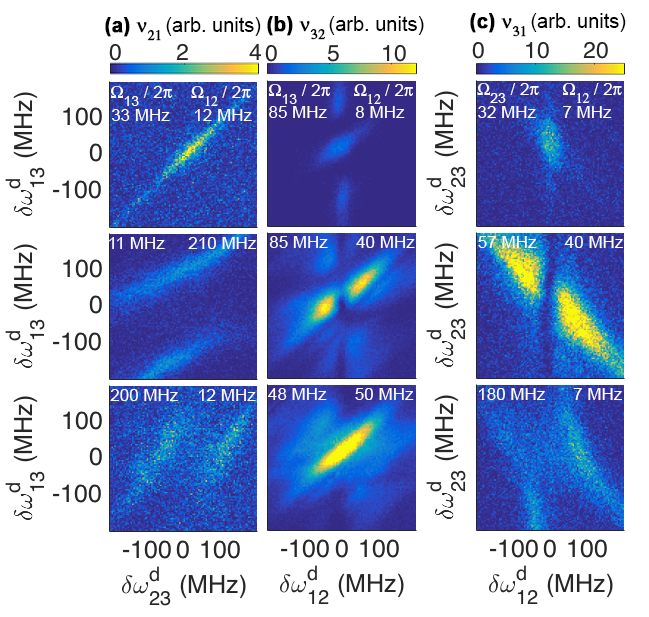
\includegraphics[width=0.85\columnwidth]{fig3_delta.png} 
\caption{Поток фотонов в когерентном излучении  $\nu^{em}$ (относительные единицы) как функция частотной отстройки $\delta\omega^{d}$ какдого из двух возбуждающих сигналов с амплитудами $\Omega_{ij}$. (a) Излучаемый поток фотонов при переходе $\ket{2}\rightarrow \ket{1}$, $\nu^{em}_{21}$ при отмеченных значениях амплитуд $\Omega_{13}$, $\Omega_{23}$. (b) Излучаемый поток фотонов от перехода $\ket{3}\rightarrow \ket{2}$, $\nu^{em}_{32}$, при амплитудах внешних полей $\Omega_{13}$, $\Omega_{12}$. (c): Излучаемый поток фотонов вблизи перехода $\ket{3}\rightarrow \ket{1}$, $\nu^{em}_{31}$, при амплитудах Раби внешних полей $\Omega_{12}$, $\Omega_{23}$.}
\label{fig:exp_em}
\end{figure}

Рис.~\ref{fig: 3wm_regimes}(d) отражает зависимость мощности пика когерентного излучения как функцию отстройки частоты возбуждения, $\delta\omega_{23}^d$, выраженную как фотонный поток (в относительных единицах), 
$\nu^{em}_{21}=\frac{P(\omega)}{\hbar\omega}$, для случая малой накачки: $\Omega_{13}\ll \gamma_{13}$, $\Omega_{23}\ll\gamma_{23}$, где $\gamma_{ij}$ --- скорости дефазировки. Отметим, что мы работаем только с эластичным излучением атома. Каждая точка на экспериментальной зависимости на Рис.~\ref{fig: 3wm_regimes}(d) соответствует узкому пику излучения, полученному при данном значении отстройки.

Измерения представленного на Рис.~\ref{fig: 3wm_regimes}(d) пика в зависимости от $\delta\omega_{23}$ производились также при различных значениях амплитуды поля $\Omega_{13}$, тогда как величина поля $\Omega_{23}$ не изменялась. При больших амплитудах наблюдалось расщепление пика, которое можно объяснить расщеплением уровней вследствие увеличения амплитуды, что приводит к новым собственным состоянием атома и поля, или так называемым <<одетым>> состояниям. Это расщепление было исследовано при помощи измерения зависимости эластичного излучения от двух отстроек ($\delta\omega_{13}, \delta\omega_{23}$) для некоторых произвольных амплитуд полей. Как можно увидеть на Рис.~\ref{fig:exp_em}, направление расщепления определяется амплитудой более сильного драйва: $\Omega_{13}\ll\Omega_{23}$ приводит к расщеплению уровня $\ket{1}$, а $\Omega_{23}\gg\Omega_{13}$ приводит к расщеплению уровня $\ket{2}$. Наблюдаемые в этих случаях паттерны расщепления повернуты друг относительно друга на \ang{90}, см. две нижние панели на Рис.~\ref{fig:exp_em}(a).

Аналогичным образом мы накачиваем переход между $\ket{3}$ и $\ket{1}$ волной накачки с частотой $\omega_{31}^{d}=\omega_{31}+\delta\omega_{31}$, а также переход между $
\ket{2}$ и $\ket{1}$ на частоте $\omega_{21}^{d}=\omega_{21}+\delta\omega_{21}$. Получаемая система описывается гамильтонианом, форма которого аналогична \eqref{H1}:
\begin{equation}
	\begin{aligned}
		H={}&-\hbar(\delta\omega_{21}\sigma_{22}+\delta\omega_{31}\sigma_{33})\\
		&-\hbar\left[\frac{\Omega_{12}}{2}(\sigma_{12}+\sigma_{21})+\frac{\Omega_{13}}{2}(\sigma_{32}+\sigma_{23})\right].
	\end{aligned}
\label{H2}
\end{equation}
В данной схеме накачки, измеряется мощность когерентного излучения между состояниями $\ket{3}$ и $\ket{2}$, $V_{32}^{\text{em}}$, которая излучается вблизи частоты $\omega_{32}/2\pi=8.35$~ГГц. Измеряется зависимость этого излучения от независимо изменяющихся отстроек $\delta\omega^{\text{d}}_{13}$ и $\delta\omega^{\text{d}}_{12}$ для нескольких характерных амплитуд драйва $\Omega_{13}$ и $\Omega_{12}$, см. Рис.~\ref{fig:exp_em}(b). На качественном уровне результат зависимость выглядит более сложной, чем для предыдущей схемы накачки. Из анализа численного решения (о котором будет подробнее сказано ниже) становится ясно, что когерентное излучение от атома с накачкой переходов $\ket{1}-\ket{2}$ и $\ket{1}-\ket{3}$ зависит от значений констант релаксации и дефазировки каждого из трех переходов. Яркая диагональная линия, появляющаяся на втором и третьем графике Рис.~\ref{fig:exp_em}(b), значительно зависит от скорости дефазировки $\gamma_{23}$, тогда как вертикальная линия на этих же графиках изменяется в зависимости от $\gamma_{12}$. Отметим, что численное моделирование позволяет задать параметры независимо друг от друга, тогда как в эксперименте эта произвольность ограничена. В частности, релаксация и дефазировка для более высоких уровней, как правило, происходят быстрее по сравнению с более низкими уровнями. 

Для восстановления полной картины трехволнового смешения мы также повторяем вышеописанные измерения для преобразования частоты вверх, когда атом возбуждается вблизи частот $\omega_{21}$ и $\omega_{32}$ и при этом излучает вблизи частоты $\omega_{31}$. Гамильтониан записывается аналогично предыдущим случаям: 
\begin{equation}
	\begin{aligned}
		H={}&-\hbar(\delta\omega_{21}\sigma_{11}+\delta\omega_{32}\sigma_{33})\\
		&-\hbar\left[\frac{\Omega_{12}}{2}(\sigma_{12}+\sigma_{21})+\frac{\Omega_{23}}{2}(\sigma_{32}+\sigma_{23})\right].
	\end{aligned}
\label{H3}
\end{equation}
Результат измерений когерентного сигнала на суммарной частоте представлен на Рис.~\ref{fig:exp_em}(c), в зависимости от отстроек и амплитуд драйвов. Отметим, что в эксперименте не обнаружено когерентного сигнала на разности частот $\omega_{23}-\omega_{12}$, что подтверждает квантовый характер трехволнового смешения. 
\section{Численный расчет амплитуды боковой компоненты}

Представленные в предыдущем разделе экспериментальные результаты могут быть просимулированы в полном объеме при помощи решения основного квантового уравнения для каждого из гамильтонианов (\labelcref{H1,H2,H3}). При этом Линдбладовский член выглядит следующим образом:
\begin{equation}
	\begin{aligned}
		L[\rho]={}&(\Gamma_{31}\rho_{33}+\Gamma_{21}\rho_{22})\sigma_{11}+(\Gamma_{32}\rho_{33}-\Gamma_{21}\rho_{22})\sigma_{22}\\
		&-(\Gamma_{31}\rho_{33}+\Gamma_{23}\rho_{22})\sigma_{33}-\sum_{i\neq j} \gamma_{ij}\rho_{ij}\sigma_{ij}.
	\end{aligned}
\end{equation}
Здесь $\gamma_{ij}=\gamma_{ji}$ --- константы дефазировки, уменьшающие когерентности между уровнями $i$ и $j$ а $\Gamma_{ij}$ --- константы релаксации с уровня $i$ на уровень $j$. Пытаясь привести в максимальное соответствие результатов симуляции с экспериментальными данными, мы получаем набор результатов, представленных на Рис.~\ref{fig:4}. Изображенные цветовые карты получены при $\Gamma_{21}/2\pi=8$ МГц, $\gamma_{21}/2\pi=8$ МГц, $\Gamma_{32}/2\pi=38$ МГц, $\gamma_{32}/2\pi=42$ МГц, $\Gamma_{31}/2\pi=41$ МГц, и $\gamma_{31}/2\pi=39.5$ МГц, что примерно соответствует параметрам образца, получаемым из других измерений. Можно отметить, что данные соотношения констант релаксации и дефазировки отражают достаточно типичную для потокового кубита ситуацию, когда при отходе от оптимального положения по потоку $\delta\Phi=\Phi_0/2$ значительно возрастает потоковый шум, а соответственно, и ухудшается когерентность каждого из переходов кубита. Как следствие, мы значительно отходим от предела излучательной дефазировки $\gamma_{ij}=\Gamma_{ij}/2$. С другой стороны, очевидно, что если $\gamma_{ij} \gg \Gamma_{ij}$, то никакой когерентной динамики в излучаемом поле наблюдаться не может. Поэтому изложенный способ создания $\Delta$-системы не является наилучшим, и ему может быть предложена альтернатива, в первую очередь направленная на сохранение когерентности. 
\begin{figure}[!hbt]
	\centering
	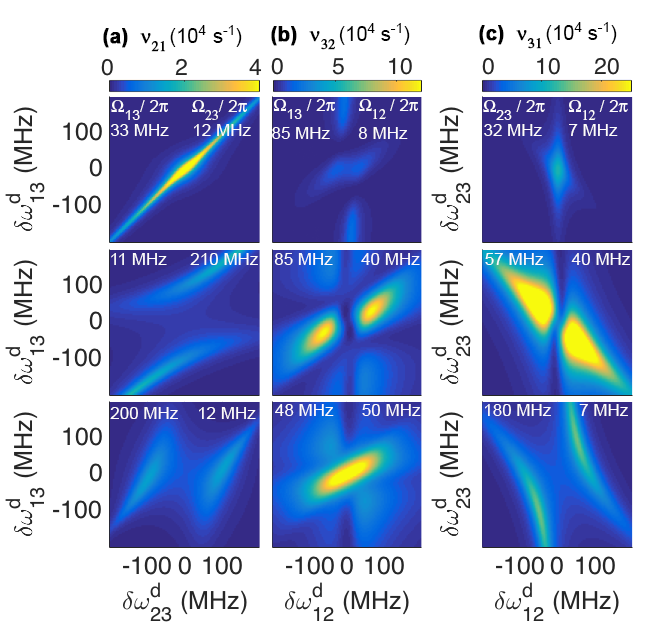
\includegraphics[width=0.85\columnwidth]{fig4-new.png} 
	\caption[Результат численного моделирования когерентной эмиссии, выраженный в единицах фотонного потока ]{Результат численного моделирования когерентной эмиссии, выраженный в единицах фотонного потока $\nu_{em}$ как функция отстроек $\delta\omega^{d}$ двух волн с амплитудами $\Omega_{ij}$ отраженных в подписях поверх панелей.(a) Излучаемый поток фотонов при переходе $\ket{2}\rightarrow \ket{1}$, $\nu^{em}_{21}$ при отмеченных значениях амплитуд $\Omega_{13}$, $\Omega_{23}$. (b) Излучаемый поток фотонов от перехода $\ket{3}\rightarrow \ket{2}$, $\nu^{em}_{32}$, при амплитудах внешних полей $\Omega_{13}$, $\Omega_{12}$. (c): Излучаемый поток фотонов вблизи перехода $\ket{3}\rightarrow \ket{1}$, $\nu^{em}_{31}$, при амплитудах Раби внешних полей $\Omega_{12}$, $\Omega_{23}$.}
	\label{fig:4}
\end{figure}

Заключая, мы продемонстрировали трехволновое смешение в форме когерентного преобразования частоты при помощи одиночного трехуровневого искусственного $\Delta$-атома. Принципиальное отличие нашего устройства от ранее использованных параметрических нелинейных устройствах на основе джозефсоновских переходов состоит в том, что смешение происходит на переходах искусственного атома, находящегося в квантовом режиме, что и определяет свойства рассеянного на атоме излучения. Принципиальным требованием является дипольная разрешенность всех переходов атома, что практически не встречается в природных атомах из-за правил отбора, однако легко реализуется при помощи потокового кубита. Мы надеемся, что полученные результаты найдут применение в создании фотонных сетей и устройств квантовой сверхпроводниковой электроники. 

Следующая глава диссертационной работы посвящена разработке источника одиночных фотонов на базе сверхпроводникового потокового кубита, несимметрично связанного с двумя одномерными полупространствами. Будет показаны результаты многотоновой спектроскопии источника, которая позволяет увидеть большое количество переходов между энергетическими уровнями кубита, а также изучить расщепление Аутлера-Таунса при выборочном драйве переходов. 
 
           % Глава 5
\chapter{Кубит как источник неклассического излучения}
Сверхпроводниковые кубиты обладают набором интересных свойств, которые позволяют контролируемым образом получить сильную связь квантовой системы и распространяющегося в волноводе поля без использования высокодобротных резонаторов. В частности, пример перспективной архитектуры для реализации микроволновой фотоники и электроники представляет схема, в которой единичный искусственный атом связывается с двумя полубесконечными линиями, которые не связаны друг с другом в отсутствии атома. При этом связь делается асимметричной. Это означает, что одна из линий, которую мы будем называть линией излучения, связана с кубитом сильным образом. Связь с линией излучения характеризуется константой распада $\Gamma_e\approx 2-20$~МГц, и она заведомо доминирует над остальными каналами распада и чистой дефазировки. Другая линия, которую мы будем называть линией контроля, размещается таким образом, что связь $\Gamma_c\ll\Gamma_e$ пренебрежимо мала. Однако, сильное поле в линии контроля может дать достаточную частоту Раби для быстрого возбуждения кубита, который сразу же начинает распадаться в линию излучения, таким образом создавая поле в этой линии. Одним из перспективных приложений таких систем может стать генерация неклассического распространяющегося света: например, успешно продемонстрирована генерация одиночных фотонов по требованию \cite{peng2016tuneable,Shaped_SPS,PechalShaped} и двух корреллированных и излучаемых в каскадном процессе фотонов, \cite{Wallraff_entangledPhotons}. В некоторых из этих работ в качестве перехода используется два нижних уровня потокового кубита, тогда как в других работах излучение идет с нижних уровней кубита-трансмона. Однако, остается открытым вопрос об возможности использования вышележащих уровней потокового кубита, шунтированного емкостью. 

В данном разделе мы расскажем о создании потокового кубита, асимметрично связанного с полупространствами, и изложим результаты просвечивающей спектроскопии, в которых успешно показано излучение на частотах различных кубитных переходов. Сравнивая результаты спектроскопических измерений с расчетными собственными энергиями кубитов, нам удалось восстановить картину энергетических состояний системы вплоть до третьего возбужденного уровня, что говорит о высокой степени контроля искусственного атома. Также при помощи измерения линии излучения удалось установить полную естественную ширину переходов $\ket{0}\leftrightarrows\ket{1}$ и $\ket{1}\leftrightarrows\ket{2}$ и увидеть расщепление Аутлера-Таунса при сильной накачке одного из переходов и измерении прохождения слабого пробного сигнала, настроенного на частоту другого перехода. Результаты данной работы составляют основу для разработки источников неклассического излучения микроволнового излучения на сверхпроводниковых искусственных атомах.
\section{Ассимметричная связь с двумя полупространствами}
Как было сказано выше, искусственный атом, исследуемый в данном разделе --- потоковый кубит, асимметрично связанный с двумя полубесконечными копланарными волноводами. Полезно представить оптический аналог такого размещения. Рассмотрим одиночный атом, подвешенный в трехмерном пространстве и расположенный позади крохотного отверстия, сделанного в непрозрачном экране. Предполагается, что размеры отверстия гораздо больше длины волны резонансного с атомным переходом света, поэтому при освещении экрана плоской монохроматической волной через отверстие проникают лишь экспоненциально затухающие т.н. \textit{эванесцентные} волны. Они распространяются лишь на расстояние порядка длины волны, но этого достаточно, чтобы возбудить атом за щелью. В свою очередь, возбужденный атом излучает поле в полупространство, свободное от экрана, где оно может быть задетектировано, отправлено в интерферометрическую схему или использовано в каких-либо других целях. Графическое изображение схемы представлено на Рис.~\ref{fig: hole}. 
\begin{figure}
	\centering
	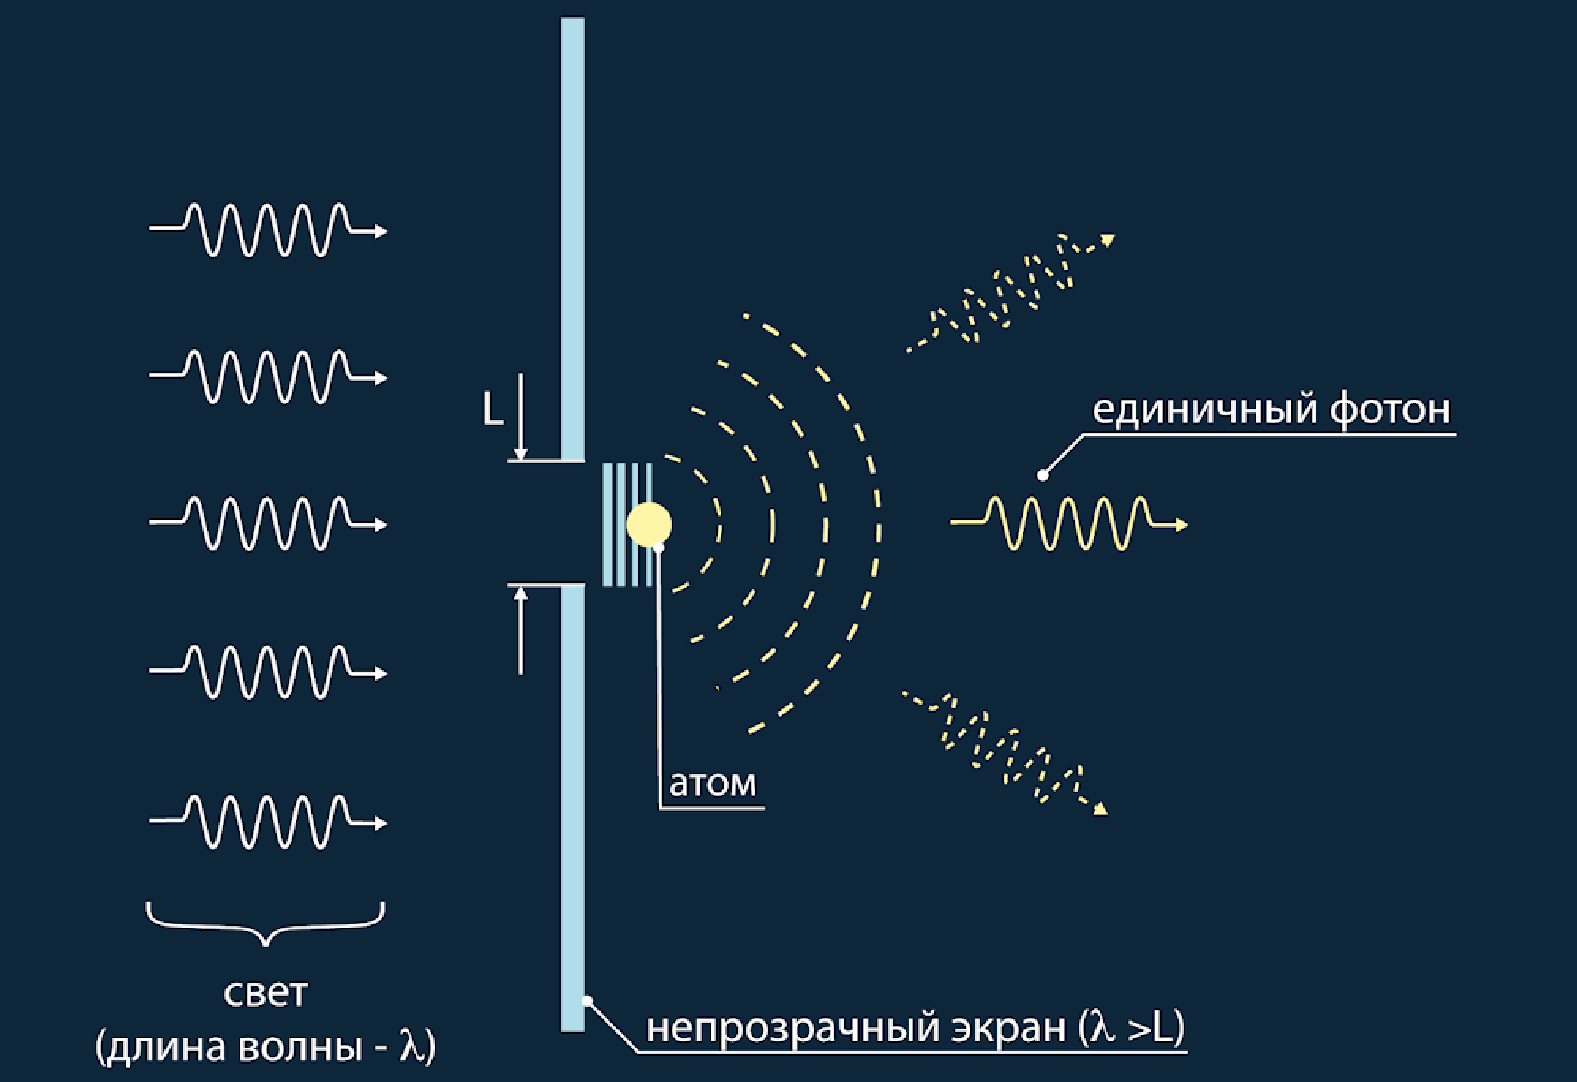
\includegraphics[width=0.85\textwidth]{sps_optical.pdf}
	\caption[Оптический аналог кубита, связанного с двумя полупространствами асимметричным образом]{Оптический аналог кубита, асимметрично связанного с двумя волноводами (подготовлено совместно с пресс-службой МФТИ). Непрозрачный экран с щелью шириной $L \ll \lambda$ образует два полупространства. Искусственный атом расположен вблизи щели справа от экрана. Плоская волна, падающая на экран слева, рассеивается на щели в виде эванесцентных волн, возбуждающих атом, который переизлучает в правое полупространство. В частности, таким образом можно осуществить генерацию одиночного фотона.}
	\label{fig: hole}
\end{figure}
Эквивалентная электрическая схема, где сверхпроводниковый потоковый кубит связан с полубесконечными волноводами, приведена на Рис.~\ref{fig: sps_scheme}(а). Емкость связи с линией контроля предполагается значительно меньшей, чем емкость связи с линией излучения. Как будет показано в следующем разделе, отношение этих емкостей является основным параметром, определяющим предельную эффективность кубита как источника одиночных фотонов. Отметим, что емкости $C_c$ и $C_e$ настолько малы, что эффективный импеданс между входной и выходной линией крайне велик и составляет порядка $10^3$ Ом. Поэтому классический импульс, налетающий слева, практически полностью отражается назад и не попадает в выходную линию. В свою очередь, в линии излучения (выходной линии) присутствует только поле, излучаемое атомом, поскольку связь атома и поля в правом волноводе достаточно сильная. 
\begin{figure}
	\centering
	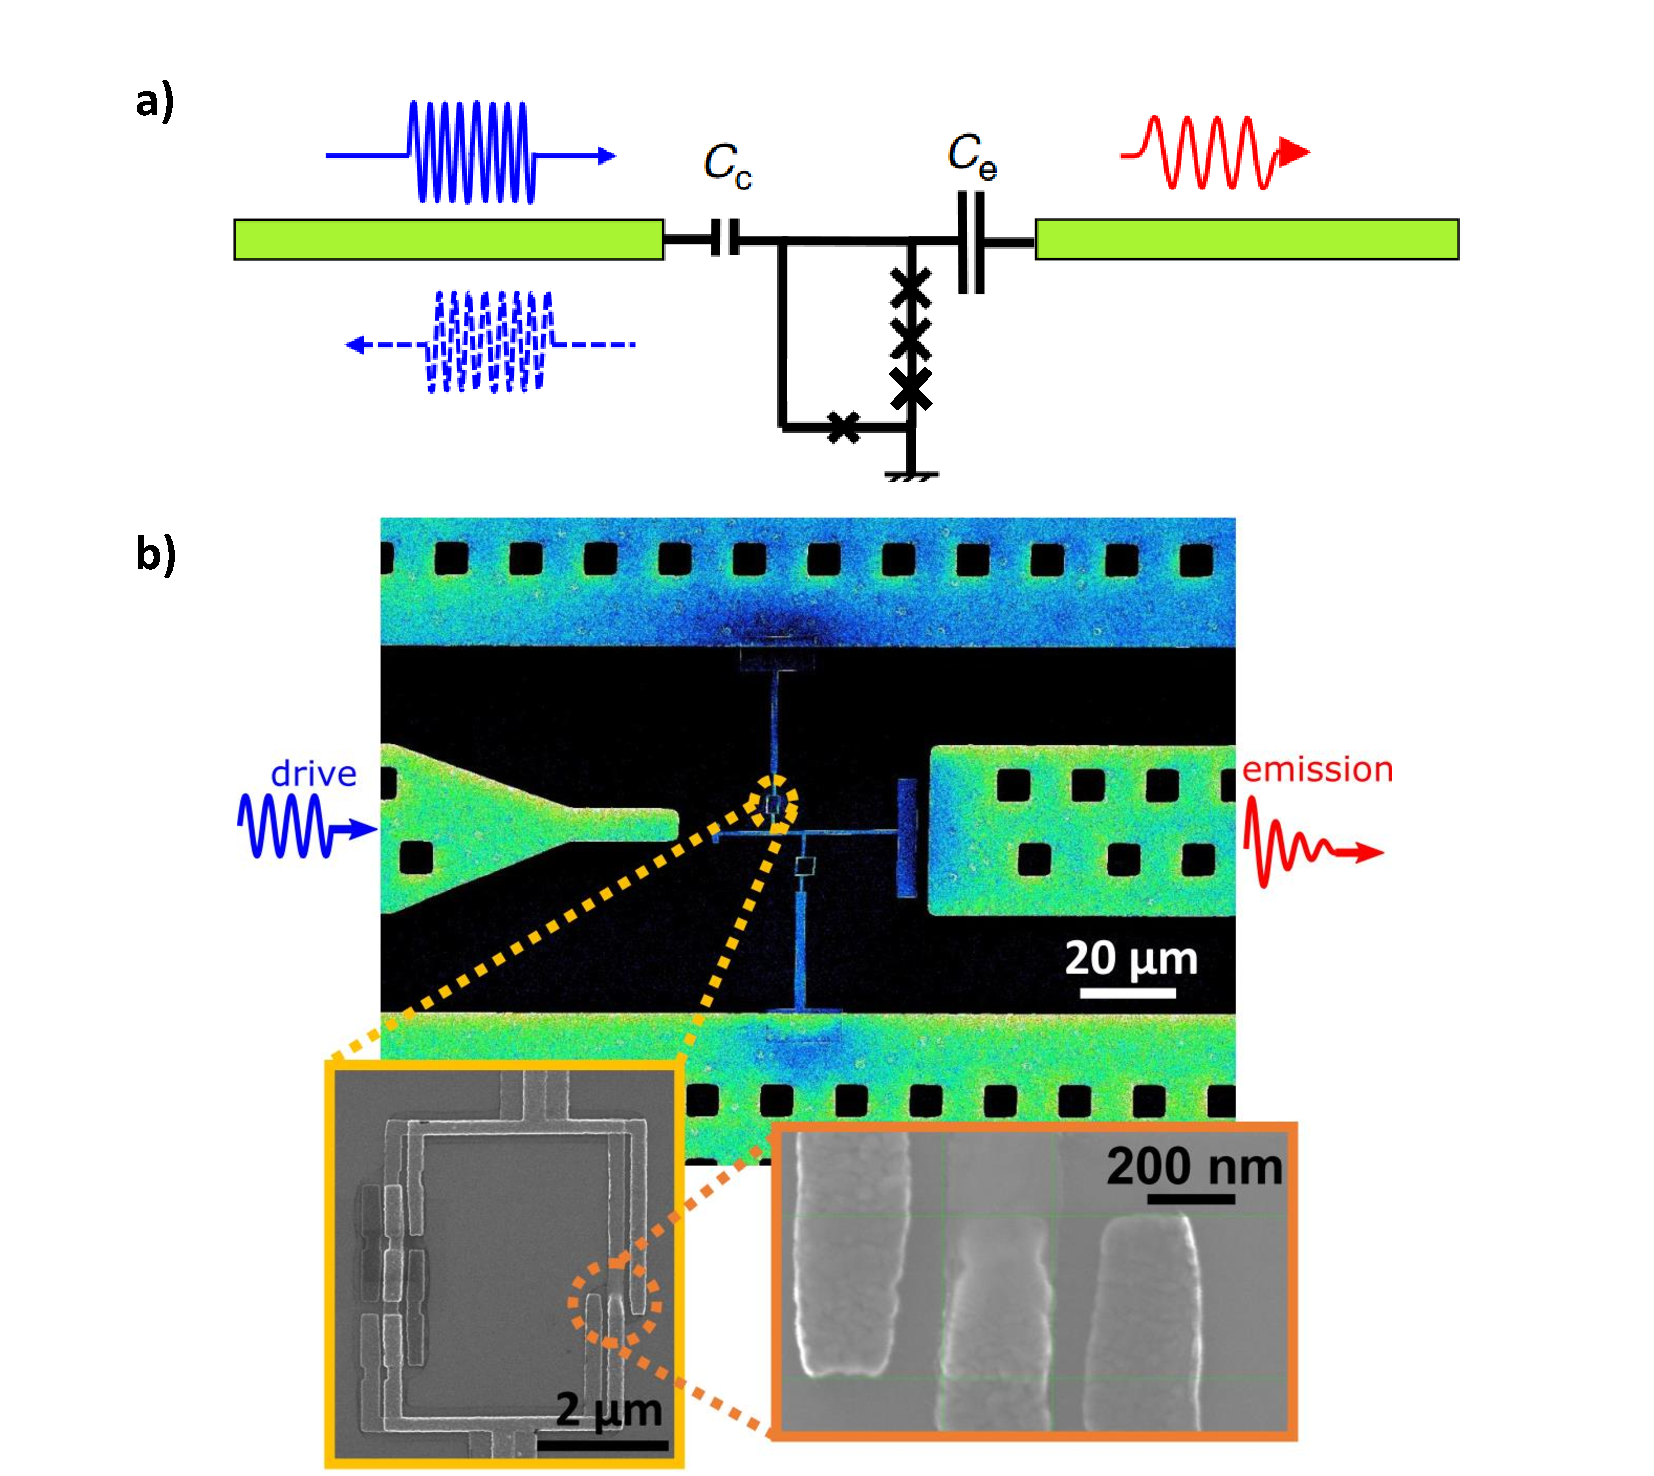
\includegraphics[width=1\textwidth]{SPS_schemes.pdf}
	\caption[Принципиальная электрическая схема и электронное изображение кубита, связанного с двумя полупространствами]{(a) - принципиальная электрическая схема потокового кубита, связанного с линией контроля при помощи емкости $C_c$ и линией излучения через емкость $C_e$. Классический управляющий сигнал (синяя волна) направляется в линию контроля и возбуждает атом, после чего он излучает в линию справа (красная волна). Схема адаптирована из \cite{peng2016tuneable} c разрешения авторов. (b) Изображение экспериментального образца кубита в сканирующем электронном микроскопе.}
	\label{fig: sps_scheme}
\end{figure}
В следующем разделе мы подробно рассмотрим параметры экспериментального образца кубита, используемого для наблюдения многоуровневой спектроскопии атома через линию излучения.
\section{Дизайн и параметры прибора}
Наш прибор представляет собой потоковый сверхпроводящий кубит с четыремя джозефсоновскими переходами \cite{Astafiev2010resonance,qiu2016four}, сфабрикованный при помощи стандартной методики двухуглового теневого напыления, см. Рис.~\ref{fig: sps_scheme}(b). Размеры трёх больших переходов одинаковы и равны $0.2\times0.8$~$\mu m $, а четвёртый в $\alpha \approx 0.35$ раз меньше по площади.  Один конец $\alpha$-перехода заземлён, а другой связан с линиями передачи. Входная линия присоединена к атому через небольшую ёмкость $C_i\approx0.5$~фФ, а большая ёмкость $C_e\approx2.8$~фФ соединяет атом и считывающую линию. Тогда эффективная ёмкость $\alpha$-перехода является суммой его собственной ёмкости $C_\alpha \approx 2.5$~fF  и двух связывающих ёмкостей ($C_\alpha + C_i + C_e$). Величина незатухающего тока $I_p=18$~nA в петле меньше, чем в обычных потоковых кубитах, что делает его менее чувствительным к шуму магнитного поля. Это приводит к значительному увеличению времени дефазировки \cite{yan2016flux}, но уменьшает ангармонизм уровней кубита, как и в кубитах типа трансмон \cite{koch2007charge}. Полученной в наших экспериментах величины ангармонизма порядка $1.5$~ГГц достаточно для сохранения верности двухуровневого приближения, даже на высоких возбуждающих мощностях. В то же время, более высокие уровни $\ket{2}$ and $\ket{3}$ сдвигаются вниз по энергии, так что частоты $\ket{1} \leftrightarrow \ket{2}$ and $\ket{2} \leftrightarrow \ket{3}$ оказываются в полосе работы HEMT-усилителей (1-12 ГГц), и переходы могут быть изучены напрямую.
\section{Описание схемы эксперимента}
Для измерений образец загружается в держатель с микроволновыми копланарными линиями. Держатель присоединяется к нижней части криостата растворения Bluefors-LD250 и охлаждается до температуры 15 мК. При такой температуре $k_B T \ll \hbar \omega_{01}$, и атом находится в невозбуждённом состоянии $\ket{0}$. Сильная связь между атомом и выходной линией достигается, если частота безызлучательного перехода $\Gamma_{\text{NR}}$ состояния $\ket{1}$ много меньше естественной ширины линии $\Gamma^{01}_{1}$, обусловленной преимущественно спонтанной эмиссией в считывающую линию. В эксперименте, отличном от нашего: одиночный атом в линии передачи \cite{Astafiev2010resonance,Delsing2013microwave1Dspace} --- это выражается в практически полном отражении достаточно слабой микроволновой волны с частотой $\omega$, близкой к $\omega_{01}=(E_1 - E_0)/\hbar$: коэффициент отражения $r$ может достигнуть единицы, если $\omega = \omega_{01}$, однако далеко от резонанса $r$~=~0. Это означает, что свет может полностью рассеяться на одиночной квантовой системе. В нашей схеме с асимметричной связью атома с двумя полупространствами резонансное возбуждение приходит со стороны входной линии. Излучение возбуждённого кубита может уйти в любую из линий, однако, как это было показано в \cite{peng2016tuneable}, переизлучение происходит в считывающую линию с эффективностью $1-C^2_{i}/C^2_{e} \approx$~0.97 в случае отсутствия безызлучательной составляющей и дефазировки. В теории, за счёт увеличения отношения ёмкостей эффективность может быть сколь угодно близкой к единице. Тогда наша система будет работать как источник одиночных микроволновых фотонов, если подать на вход возбуждающий $\pi$-импульс.
В наших экспериментах мы изучаем также другое свойство нашей системы: когерентное излучение атома. Так как входная и выходная линии слабо связаны друг с другом из-за рассогласования импедансов: $|Z_s| = 1/\omega_{01} C_{i} \approx 6 \cdot10^4$~Ом много больше импеданса линии $Z_0=50$~Ом --- подавляющая часть входной мощности отражается назад. Поэтому состояние поля в считывающей линии будет определяться тем, что излучает атом. Так как наш искусственный атом --- одиночная квантовая система, то и излучаемое поле в общем случае существенно неклассическое. Соответственно, изучение спектра и интенсивности когерентных излученных волн позволяет извлекать информацию об уровнях энергии искусственного атома. Для детектирования амплитуды и фазы когерентного излучения атома используется ВАЦ, выход которого через гетеродинную схему подключен к входной линии, а вход подключен к линии излучения.

\section{Многоуровневая спектроскопия источника}
Спектроскопические измерения начинаются с того, что мы находим частоту перехода $\ket{0} \leftrightarrow \ket{1}$, подавая на нашу систему микроволновый сигнал на частоте $\omega$, изменяемой в широком диапазоне, и меряя пропускание системы. Также мы меняем магнитное поле через петлю потокового кубита. На Рис.~\ref{spectr}a) изображён типичный спектр: интенсивность на выходе из системы, измеренная при помощи ВАЦ, как функция внешнего поля и частоты возбуждающей гармоники. Максимальная интенсивность на выходе из атома определяется его однофотонной мощностью излучения $P_{01}=\hbar\Gamma^{01}_1 \omega_{01}$, которая, в свою очередь, ограничена скоростью излучения $\Gamma^{01}_1$: двухуровневая система не может излучать более чем один фотон за раз. Соответствующая максимальная входная мощность, которую рассеивает кубит, равна $P \sim P_{01} \sim 10^{-17}$~Вт. Светлая линия на Рис.~\ref{spectr}a) соответствует низшему переходу $\ket{0} \leftrightarrow \ket{1}$; такая методика позволяет обнаружить только этот переход из-за высокого ангармонизма кубита.
\begin{figure*}[htb] 
	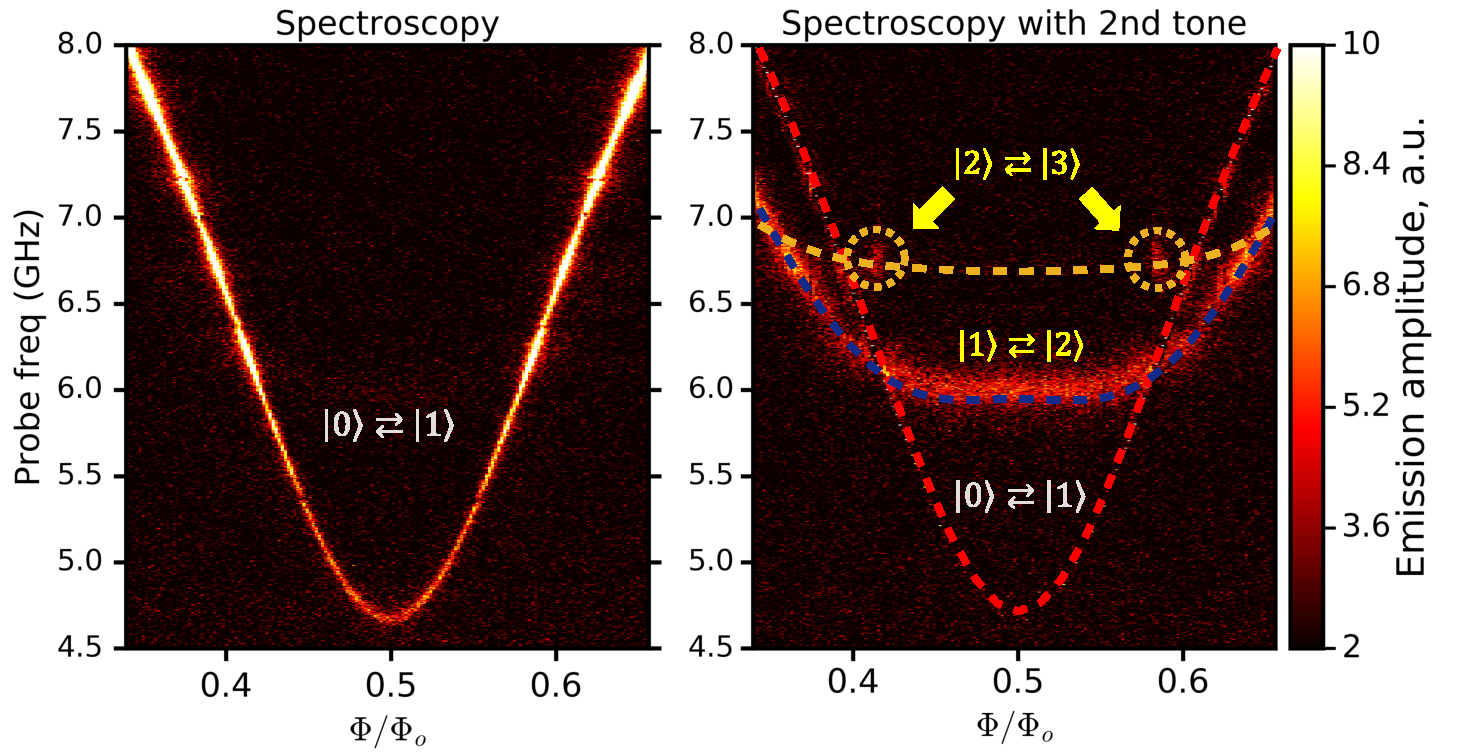
\includegraphics[width=1\textwidth]{figure_2-1} 
	\caption{Спектроскопия системы. Амплитуды излучения, измеренные с помощью VNA, как функции частоты возбуждающего поля и магнитного потока $\Phi$ через петлю кубита. (a) Напрямую измеренный переход $\ket{0}\leftrightarrow \ket{1}$. (b) Переход $\ket{1}\leftrightarrow\ket{2}$, измеренный, когда первый уровень $\ket{1}$ (красная пунктирная кривая) возбуждён приложением первого тона на частоте $\omega_{01}$. Пунктирные кривые - это численно рассчитанные уровни потокового кубита с параметрами нашего образца. Помимо этого, когда $\omega_{01}=\omega_{12}$, уровень $\ket{2}$ заселён, и видно излучение от перехода $\ket{2}\leftrightarrow\ket{3}$ (внутри жёлтых кругов)   }
	\label{spectr}
\end{figure*}
Далее, мы предлагаем метод измерения переходов между более высокими уровнями. Например, для измерения перехода $\ket{1} \leftrightarrow \ket{2}$ мы облучаем атом двумя синусоидальными сигналами: одним на частоте $\omega_{01}$ с увеличенной мощностью $\sim10^{-13}$~Вт и вторым низкой мощности $\sim P_{01}$. При этом, частота второго сигнала меняется в том же диапазоне, что и на Рис.~\ref{spectr}a. Первый сигнал насыщает состояния $\ket{0}$ и $\ket{1}$ атома до приблизительно 50\%. В такой схеме, второй сигнал может перевести атом из состояния $\ket{1}$ в $\ket{2}$, а атом начнёт излучать сигнал с частотой $\omega_{12}=(E_2 - E_1)/h$. Это подтверждается на эксперименте: на Рис.~\ref{spectr}b видна дополнительная спектральная линия, соответствующая переходу $\omega_{12}=(E_2 - E_1)/h$. Два ярких пятна на $\Phi \approx 0.42 \Phi_0$ и $\Phi \approx 0.58 \Phi_0$ (где $\Phi_0$ - квант магнитного потока) мы объясняем возбуждением уровня $\ket{3}$ системы, потому что в указанных значениях магнитного потока частота перехода $\ket{0} \leftrightarrow \ket{1}$ совпадает с частотой перехода $\ket{1} \leftrightarrow \ket{2}$. Это позволяет заселить состояние $\ket{2}$ первым тоном, в то время как второй тон при соответствии частот может заселить уровень $\ket{3}$, что и выражается в наблюдении излучения на частоте перехода $\ket{3} \leftrightarrow \ket{2}$.
\begin{figure}[tbh] 
	\centering
	\includegraphics[width=0.7\columnwidth]{figure_3-1} 
	\caption{Интенсивность когерентного излучения системы как функция входной частоты. Искусственный атом облучается монохроматическим внешним сигналов, при этом измеряется мощность упруго рассеянного света. В случае малой мощности, переход $\ket{i} \leftrightarrow \ket{j} $ имеет форму лоренциана \cite{Astafiev2010resonance} с полной шириной на половине высоты, равным $\Gamma^{ij}_1$.
	}
	\label{peaks}
\end{figure}
Из спектроскопии системы можно извлечь другие её параметры: например, времена релаксации. На Рис.~\ref{peaks} изображена зависимость коэффициента пропускания от частоты в точке вырождения по магнитному полю ($\Phi = \Phi_0/2$). Коэффициент пропускания $\ket{0}\leftrightarrow \ket{1}$ изображён на синей кривой, $\ket{1}\leftrightarrow\ket{2}$ - на красной кривой во вставке. После фитирования их лоренцианом
\begin{equation}
	P(\omega)=\frac{1}{\pi}\frac{\Gamma/2}{(\omega-\omega_0)^2+\left(\Gamma/2\right)^2},
\end{equation} 
мы извлекаем значения скоростей распада $\Gamma_{1}^{01}/2\pi=20.8$~МГц and $\Gamma_{1}^{12}/2\pi=192.4$~МГц. Эти значения позволяют, в частности, получить уже использованное значение однофотонной мощности $P_{01} \sim 10^{-17}$~Вт. Как уже было сказано, скорость перехода между произвольными состояниями атома определяется скоростью излучения в считывающую линию и может быть рассчитана, если все параметры системы известны \cite{Astafiev-quantum-amplifier,Astafiev2010resonance}.

Теоретически рассчитанный спектр системы получается из диагонализации гамильтониана четырёх джозефсоновских переходов в зарядовом базисе. Результат приведён на Рис.~\ref{spectr}b (пунктирные кривые). Спектры расссчитаны для параметров: $E_J/2\pi=35$, $E_{Cc}/2\pi=13.5$, $E_C/2\pi=19$~ГГц и $\alpha=0.31$.  Видно, что расчет отлично согласуется с экспериментом. Зарядовая энергия связи обозначена как $E_{cC} = 4e^2/2(C_c+C_e+C_s)$, где $C_s$ --- некоторая емкость на землю, в то время как $E_C$ --- зарядовая энергия каждого из больших джозефсоновских переходов. На том же рисунке приведена теоретическая кривая для перехода  $\ket{2} \leftrightarrow \ket{3}$. Как было указано ранее, в эксперименте излучение на частоте этого перехода наблюдается только при некоторых значениях потока.
После проведения спектроскопического эксперимента опишем, как исследуемый образец может быть использован в качестве источника одиночных фотонов. Для этого рассчитаем коэффициенты прохождения и отражения В аналогичной разделу \ref{sec: scatt} манере рассмотрим рассеяние поля, идущего на кубит из линии контроля либо из линии излучения, и определим коэффициенты отражения и прохождения в зависимости от частоты Раби, констант связи, дефазировки и отстройки частоты внешнего поля от частоты кубита.
\section{Эффективность прибора в качестве источника одиночных фотонов}
Для полной характеризации коэффициентов прохождения и отражения непрерывных волн достаточно использовать выражение \eqref{eq: stat_s-}, при этом нужно помнить, что стационарное состояние зависит от полной релаксации $\Gamma_1 = \Gamma_1^c + \Gamma_1^e + \Gamma_1^{\text{nr}}$. С учетом этого выражения, среднее поле в линии контроля и в линии излучения \cite{peng2016tuneable} можно вычислить следующим образом:
\begin{subequations}\label{coherentwaves}
	\begin{eqnarray}
		&x < 0: &V_{c}(x,t)=i\frac{\hbar\Gamma_1^{c}}{C_{c} \nu_{a}}\langle\sigma^{-}\rangle e^{-i\omega t - ikx}, \\
		&x > 0:  &V_{e}(x,t)=i\frac{\hbar\Gamma_1^{e}}{C_{e} \nu_{a}}\langle\sigma^{-}\rangle e^{-i\omega t + ikx},
	\end{eqnarray}
\end{subequations}
где $\nu_a$ --- атомный дипольный момент перехода 0-1. 
Из этих уравнений легко получить выражения для коэффициента отражения поля в контрольной линии $r_{\text{c}}$ и коэффициента прохождения в линию линии излучения $t_{\text{ce}}$. Однако, для определения внутренних потерь наиболее подходящим измерением является зависимость коэффициента отражения поля, направленного на кубит через линию излучения $r_{\text{e}}$, от отстройки $\delta\omega$, которая для случая $\Omega^2\ll\Gamma_1\Gamma_2$ выражается соотношением:
\begin{eqnarray}
	&r_e& = 1-\frac{\Gamma_1^e}{\Gamma_2}\frac{1}{1-i\delta\omega/\Gamma_2}.\label{re}
\end{eqnarray}
\begin{figure}[!h]
	\centering
	\includegraphics[width=0.8\textwidth]{SMITH_SPS_ver3_load6.png}
	\caption[Зависимость $r_e(\delta\omega)$, измеренная с помощью ВАЦ]{Зависимость $r_e(\delta\omega)$ для различных значений $\Omega$ потокового кубита, измеренная с помощью ВАЦ. Полученное в эксперименте значение $\left. r_e(0)\right\vert_{\Omega=0}\approx-0.4$ характеризует полную эффективность генерации одиночных фотонов как $\Gamma^e_1/2\Gamma_2 \approx 0.7$, что находится в соответствии с результатом \cite{peng2016tuneable}. }
	\label{fig: eff}
\end{figure}
Данное выражение весьма удобно для характеризации внутренних нерадиационных потерь и потерь, возникающих из-за чистой дефазировки. В самом деле, $\Gamma_2 = \Gamma_1/2 + \gamma_\phi $, а это означает, что в наиболее идеальном случае, когда $\Gamma_1^c \ll \Gamma_1^e$, $\Gamma_1^{\text{nr}}=0$~и~$\gamma_\phi=0$, зависимость $r_e(\delta\omega)$ представляется окружностью на комплексной плоскости с центром в точке $(0,0)$ и радиусом 1. В частности, удобно обратить внимание на значение $r_e(0)=-1$ в идеальном случае и не доходящим до этого значения из-за внутренних потерь на кубите. Экспериментально измеренная зависимость $r_e(\delta\omega)$ приведена на Рис.~\ref{fi: eff}. Из измерений можно заключить, что эффективность кубита в качестве источника фотонов составляет примерно 70\%. 

Дополнительно была измерена зависимость $|t_{\text{ce}}(\delta\omega)|$ при различных значениях $\Omega$. Результаты этих измерений приведены на Рис.~\ref{fig: sps_peak_from_power}. Интересно, что выражение для $t_{\text{ce}}$ совпадает с выражением \eqref{eq: refl} для амплитудного коэффициента отражения кубита в линии с точностью до сомножителя $C_c/C_e$. Поэтому данные на Рис.~\ref{fig: sps_peak_from_power} хорошо воспроизводят построенную на Рис.~\ref{fig: refl} зависимость для $|r|$. 
\begin{figure}[h]
	\centering
	\includegraphics[width=0.8\textwidth]{SPS_peak_from_power.png}
	\caption[Зависимость $t_{\text{ce}}(\delta\omega)$, измеренная с помощью ВАЦ]{Зависимость $t_{\text{ce}}(\delta\omega)$, измеренная с помощью ВАЦ для различных значений $\Omega$. Характер зависимости аналогичен $r(\delta\omega)$ для кубита в линии и описывается соотношением \eqref{eq: refl}}
	\label{fig: sps_peak_from_power}
\end{figure}
Генерация одиночных фотонов от источника требует предварительной калибровки $\pi$-импульсов, которые достигают кубита через контрольную линию и переводят его в состояние $\ket{1}$. Сигнал, сгенерированный кубитом во время распада в линию излучения, и будет являться единичным фотоном с экспоненциально затухающей огибающей, и константа ее затухания полностью определяется значением $\Gamma_1^e$. Для того, чтобы измерить профиль этой огибающей, нужно усреднить большое количество единичных временных разверток средней мощности. Таким образом, временная развертка поля после одного $\pi$-импульса, измеренная при помощи высокоскоростного $АЦП$, возводится в квадрат и результат усредняется по множественным реализациям. Поскольку соотношение <<cигнал-шум>> для измерениц излучаемого кубитом поля достаточно мало, то требуется не менее $10^6$ измерений для получения качественной огибающей. Результат измерения средней мощности от времени приведен на Рис.~\ref{fig: photon_exp}.
Из времени затухания однозначно определяется константа релаксации $\Gamma_1^e$.
\begin{figure}[h]
	\centering
	\includegraphics[width=0.6\textwidth]{photon_exp.png}
	\caption[Огибающая одиночного фотона, пропорциональная $\exp(-\Gamma^e_1 t)$]{Огибающая одиночного фотона, пропорциональная $\exp(-\Gamma^e_1 t)$, полученная после $\sim 10^6$ усреднений единичных разверток мощности. Характерное время затухания $1/\Gamma^e_1 \approx 20 $~нс, что соответствует $\Gamma^e_1/2\pi\approx8$~МГц.}
	\label{fig: photon_exp}
\end{figure}
Необходимо отметить, что статистика излучаемого кубитом света будет отличаться от одиночного фотона. Используемая схема подключения кубита к линии излучения --- постоянная емкостная связь --- не позволяет выключать связь с линией во время возбуждения кубита классическим импульсом, поэтому кубит излучает некоторое поле в процессе своего возбуждения, и это поле может иметь не однофотонный характер. Для характеризации статистики излучаемого кубитом поля через измерение корреляционных функций 
\begin{eqnarray}
	&g^{(1)}(\tau) &=\int \braket{V_1(t+\tau)V_2(t)} \,dt, \\
	&g^{(2)}(\tau) &=\int \braket{V_1^2(t+\tau)V_2^2(t)} \,dt.
\end{eqnarray}
была собрана интерференционная схема Хенбери-Брауна-Твисса \cite{confbib1}, изображенная на Рис.~\ref{fig: hbt}. С ее помощью проведены измерения корреляторов первого порядка, см. Рис.~\ref{fig: g1tau}. Корелляторы измерялись при различных последовательности управляющих импульсов: одна из них приводит кубит в состояние $\ket{1}$, а другая --- в состояние $\ket{0+1}/2$. 
\begin{figure}
	\centering
	\includegraphics[width=0.5\textwidth]{HBT.jpg}
	\caption[Схема сборки интерферометра Хенбери-Брауна-Твисса]{Схематичное изображение экспериментальной установки, реализующей интерферометрическую схему Хенбери-Брауна-Твисса для излучения от источника одиночных фотонов. Для создания импульсов используется ГИПФ, разведение сигнала по плечам интерферометра осуществляется при помощи гибридного ответвителя, который по своему функционалу аналогичен делителю пучка 50/50 в оптике. Для оцифровки данных используется АЦП.}
	\label{fig: hbt}
\end{figure}
\begin{figure}
	\centering
	\includegraphics[width=1\textwidth]{G1_meas.pdf}
	\caption[Результаты измерения $g^{(1)}(\tau)$]{Результаты измерения $g^{(1)}(\tau)$ для различных состояний кубита. Отчетливо видно, что для состояния суперпозиции фаза излучения, испускамого кубитом после различных импульсов, корреллирует друг с другом, тогда как для состояния $\ket{1}$ корелляция полей при ненулевой задержке отсутствует.}
	\label{fig: g1tau}
\end{figure}
Отчетливо определяется различный характер корреляций в зависимости от состояния поля в волноводе. Для достоверного определения однофотонности необходимо измерить корреляцию второго порядка для нулевой задержки, чтобы в случае одиночного фотона пронаблюдать полную антикорреляцию, свидетельствующую о том, что фотон целиком летит либо в первое, либо во второе плечо интерферометра. Однако, это измерение предъявляет значительные технические требования, в частности, усреднение как минимум $10^{10}$ отдельных актов испускания фотона, что требует использование ПЛИС для анализа данных, либо же гораздо менее шумящих параметрических усилителей, работающих в квантовом пределе шумов. В рамках этой работы измерение корреляционной функции второго порядка не производилось, однако, в дальнейшем планируется реализация такого измерения.

В завершение данной главы, приведем результаты экспериментального исследования расщепления Аутлера-Таунса для потокового кубита, асимметрично связанного с двумя полупространствами. 

\section{Расщепление Аутлера-Таунса}
Как было подробно рассмотрено в разделе \ref{sec: qo3ls}, для наблюдения расщепления собственных уровней системы из-за взаимодействия с полем необходимо направить на атом резонансную с одним из переходов накачку и наблюдать прохождение слабого пробного сигнала на частоте другого перехода. Результат таких измерений в двух возможных конфигурациях приведен на Рис.~\ref{fig: sps_ats}. Коэффициент прохождения для пробного сигнала вблизи частоте перехода $\ket{0}\leftrightarrow\ket{1}$ ($\ket{1}\leftrightarrow\ket{2}$) значительно меняется при увеличении амплитуды накачки $\Omega$ на частоте перехода $\ket{1}\leftrightarrow\ket{2}$ ($\ket{0}\leftrightarrow\ket{1}$). Дополнительно охарактеризовать возникновение расщепления можно при помощи измерения пропускания при нулевой отстройке, и результаты этих измерений приведены на Рис.~\ref{lines}. Расщепление уровней $\ket{0}$ и $\ket{1}$ приводит к тому, что мощность когеретного поля, излучаемого точно в резонанче с переходом $\ket{1} \leftrightarrow \ket{2}$, значительно падает. Максимум этой мощности практически точно совпадает с условием $\Omega_01 = \Gamma_1^{01}$, отмеченного на Рис.~\ref{lines} оранжевой вертикальной линией, положение которой определено независимо из осцилляций Раби. Таким образом, мы получаем своеобразную версию критерия Релея: свидетельством расхождения пиков на расстояние, большее их относительной ширины $\sim \Gamma_1$, является достижение максимума резонансно излучаемого поля и его последущее спадание при дальнейшем увеличении мощности. 
\begin{figure}[h]
	\centering
	\includegraphics[width=1\textwidth]{SPS_ATS.pdf}
	\caption[Расщепления Аутлера-Таунса в асимметрично связанном потоковом кубите.]{Расщепления Аутлера-Таунса в асимметрично связанном потоковом кубите. Кривые для различных значений мощности сдвинуты по вертикали друг относительно друга.}
	\label{fig: sps_ats}
\end{figure}
\begin{figure}[!ht] 
	\centering
	\includegraphics[width=0.7\textwidth]{figure_4-2.pdf} 
	\caption[Зависимость излучения на частоте перехода $\ket{1}\leftrightarrow \ket{2}$ от мощности первого тона на частоте перехода $\ket{0}\leftrightarrow \ket{1}$]{Зависимость излучения на частоте перехода $\ket{1}\leftrightarrow \ket{2}$ от мощности первого тона на частоте перехода $\ket{0}\leftrightarrow \ket{1}$. Оптимальная накачка (наибольшее излучение) соответствует случаю $\Omega_{01} \approx \Gamma_1^{01}$.}
	\label{lines}
\end{figure} 

В данной главе приведены результаты исследования одиночного сверхпроводникового потокового кубита, связанного с двумя полупространствами несимметричным образом. Во-первых, мы продемонстрировали новый способ спектроскопии искусственных атомов, основанный на разделении возбуждающей и излученной волны благодаря асимметричной связи атома с двумя линиями с открытыми концами. Когерентное излучение детектируется со стороны считывающей линии, тогда как атом управляется со стороны более слабо связанной линией контроля. Используя эту методику, мы измерили спектр трёхуровневой системы и определили её времена релаксации. Этот метод будет полезен для приложений в микроволновой квантовой оптике на чипах. Также мы исследовали образец в режиме генерации одиночных фотонов и состояний суперпозиции, в частности, определили эффективность генерации при помощи измерения коэффициента отражения сигнала от кубита, а также измерили огибающую одиночных фотонов во времени и корелляционные функции первого порядка. Эти результаты послужат заделом к созданию более эффективных источников одиночных фотонов и их использованию в комбинированных схемах с большим количеством атомов и волноводов на чипе, что откроет путь для реализации когерентной квантовой СВЧ-электроники на сверхпроводниковых квантовых цепей.           % Глава 6
%\chapter{Оформление различных элементов} \label{chapt1}

\section{Форматирование текста} \label{sect1_1}

Мы можем сделать \textbf{жирный текст} и \textit{курсив}.

%\newpage
%============================================================================================================================

\section{Ссылки} \label{sect1_2}
Сошлёмся на библиографию.
Одна ссылка: \cite[с.~54]{Sokolov}\cite[с.~36]{Gaidaenko}.
Две ссылки: \cite{Sokolov,Gaidaenko}.
Много ссылок: %\cite[с.~54]{Lermontov,Management,Borozda} % такой «фокус» вызывает biblatex warning относительно опции sortcites, потому что неясно, к какому источнику относится уточнение о страницах, а bibtex об этой проблеме даже не предупреждает
\cite{Lermontov,Management,Borozda,Marketing,Constitution,FamilyCode,Gost.7.0.53,Razumovski,Lagkueva,Pokrovski,Sirotko,Lukina,Methodology,Encyclopedia,Nasirova,Berestova,Kriger}.
И~ещё немного ссылок:
\cite{Article,Book,Booklet,Conference,Inbook,Incollection,Manual,Mastersthesis,Misc,Phdthesis,Proceedings,Techreport,Unpublished}.
\cite{medvedev2006jelektronnye, CEAT:CEAT581, doi:10.1080/01932691.2010.513279,Gosele1999161,Li2007StressAnalysis, Shoji199895,test:eisner-sample,AB_patent_Pomerantz_1968,iofis_patent1960}

%Попытка реализовать несколько ссылок на конкретные страницы для стандартной реализации:[\citenum{Sokolov}, с.~54; \citenum{Gaidaenko}, с.~36].

%Несколько источников мультицитата (только в biblatex)
%\cites[vii--x, 5, 7]{Sokolov}[v"--~x, 25, 526]{Gaidaenko} поехали дальше

Ссылки на собственные работы:~\cite{vakbib1, confbib1}

Сошлёмся на приложения: Приложение \ref{AppendixA}, Приложение \ref{AppendixB2}.

Сошлёмся на формулу: формула \eqref{eq:equation1}.

Сошлёмся на изображение: рисунок \ref{img:knuth}.

%\newpage
%============================================================================================================================

\section{Формулы} \label{sect1_3}

Благодаря пакету \textit{icomma}, \LaTeX~одинаково хорошо воспринимает в качестве десятичного разделителя и запятую ($3,1415$), и точку ($3.1415$).

\subsection{Ненумерованные одиночные формулы} \label{subsect1_3_1}

Вот так может выглядеть формула, которую необходимо вставить в строку по тексту: $x \approx \sin x$ при $x \to 0$.

А вот так выглядит ненумерованая отдельностоящая формула c подстрочными и надстрочными индексами:
\[
(x_1+x_2)^2 = x_1^2 + 2 x_1 x_2 + x_2^2
\]

При использовании дробей формулы могут получаться очень высокие:
\[
  \frac{1}{\sqrt{2}+
  \displaystyle\frac{1}{\sqrt{2}+
  \displaystyle\frac{1}{\sqrt{2}+\cdots}}}
\]

В формулах можно использовать греческие буквы:
\[
\alpha\beta\gamma\delta\epsilon\varepsilon\zeta\eta\theta\vartheta\iota\kappa\lambda\\mu\nu\xi\pi\varpi\rho\varrho\sigma\varsigma\tau\upsilon\phi\varphi\chi\psi\omega\Gamma\Delta\Theta\Lambda\Xi\Pi\Sigma\Upsilon\Phi\Psi\Omega
\]

\def\slantfrac#1#2{ \hspace{3pt}\!^{#1}\!\!\hspace{1pt}/
  \hspace{2pt}\!\!_{#2}\!\hspace{3pt}
} %Макрос для красивых дробей в строчку (например, 1/2)
Для красивых дробей (например, в индексах) можно добавить макрос
\verb+\slantfrac+ и писать $\slantfrac{1}{2}$ вместо $1/2$.
%\newpage
%============================================================================================================================

\subsection{Ненумерованные многострочные формулы} \label{subsect1_3_2}

Вот так можно написать две формулы, не нумеруя их, чтобы знаки равно были строго друг под другом:
\begin{align}
  f_W & =  \min \left( 1, \max \left( 0, \frac{W_{soil} / W_{max}}{W_{crit}} \right)  \right), \nonumber \\
  f_T & =  \min \left( 1, \max \left( 0, \frac{T_s / T_{melt}}{T_{crit}} \right)  \right), \nonumber
\end{align}

Выровнять систему ещё и по переменной $ x $ можно, используя окружение \verb|alignedat| из пакета \verb|amsmath|. Вот так: 
\[
    |x| = \left\{
    \begin{alignedat}{2}
        &&x, \quad &\text{eсли } x\geqslant 0 \\
        &-&x, \quad & \text{eсли } x<0
    \end{alignedat}
    \right.
\]
Здесь первый амперсанд (в исходном \LaTeX\ описании формулы) означает выравнивание по~левому краю, второй "--- по~$ x $, а~третий "--- по~слову <<если>>. Команда \verb|\quad| делает большой горизонтальный пробел.

Ещё вариант:
\[
    |x|=
    \begin{cases}
    \phantom{-}x, \text{если } x \geqslant 0 \\
    -x, \text{если } x<0
    \end{cases}
\]

Кроме того, для  нумерованых формул \verb|alignedat|  делает вертикальное
выравнивание номера формулы по центру формулы. Например,  выравнивание компонент вектора:
\begin{equation}
 \label{eq:2p3}
 \begin{alignedat}{2}
{\mathbf{N}}_{o1n}^{(j)} = \,{\sin} \phi\,n\!\left(n+1\right)
         {\sin}\theta\,
         \pi_n\!\left({\cos} \theta\right)
         \frac{
               z_n^{(j)}\!\left( \rho \right)
              }{\rho}\,
           &{\boldsymbol{\hat{\mathrm e}}}_{r}\,+   \\
+\,
{\sin} \phi\,
         \tau_n\!\left({\cos} \theta\right)
         \frac{
            \left[\rho z_n^{(j)}\!\left( \rho \right)\right]^{\prime}
              }{\rho}\,
            &{\boldsymbol{\hat{\mathrm e}}}_{\theta}\,+   \\
+\,
{\cos} \phi\,
         \pi_n\!\left({\cos} \theta\right)
         \frac{
            \left[\rho z_n^{(j)}\!\left( \rho \right)\right]^{\prime}
              }{\rho}\,
            &{\boldsymbol{\hat{\mathrm e}}}_{\phi}\:.
\end{alignedat}
\end{equation}

Ещё об отступах. Иногда для лучшей <<читаемости>> формул полезно
немного исправить стандартные интервалы \LaTeX\ с учётом логической
структуры самой формулы. Например в формуле~\ref{eq:2p3} добавлен
небольшой отступ \verb+\,+ между основными сомножителями, ниже
результат применения всех вариантов отступа:
\begin{align*}
\backslash! &\quad f(x) = x^2\! +3x\! +2 \\
  \mbox{по-умолчанию} &\quad f(x) = x^2+3x+2 \\
\backslash, &\quad f(x) = x^2\, +3x\, +2 \\
\backslash{:} &\quad f(x) = x^2\: +3x\: +2 \\
\backslash; &\quad f(x) = x^2\; +3x\; +2 \\
\backslash \mbox{space} &\quad f(x) = x^2\ +3x\ +2 \\
\backslash \mbox{quad} &\quad f(x) = x^2\quad +3x\quad +2 \\
\backslash \mbox{qquad} &\quad f(x) = x^2\qquad +3x\qquad +2
ece\end{align*}


Можно использовать разные математические алфавиты:
\begin{align}
\mathcal{ABCDEFGHIJKLMNOPQRSTUVWXYZ} \nonumber \\
\mathfrak{ABCDEFGHIJKLMNOPQRSTUVWXYZ} \nonumber \\
\mathbb{ABCDEFGHIJKLMNOPQRSTUVWXYZ} \nonumber
\end{align}

Посмотрим на систему уравнений на примере аттрактора Лоренца:

\[ 
\left\{
  \begin{array}{rl}
    \dot x = & \sigma (y-x) \\
    \dot y = & x (r - z) - y \\
    \dot z = & xy - bz
  \end{array}
\right.
\]

А для вёрстки матриц удобно использовать многоточия:
\[ 
\left(
  \begin{array}{ccc}
  	a_{11} & \ldots & a_{1n} \\
  	\vdots & \ddots & \vdots \\
  	a_{n1} & \ldots & a_{nn} \\
  \end{array}
\right)
\]


%\newpage
%============================================================================================================================
\subsection{Нумерованные формулы} \label{subsect1_3_3}

А вот так пишется нумерованая формула:
\begin{equation}
  \label{eq:equation1}
  e = \lim_{n \to \infty} \left( 1+\frac{1}{n} \right) ^n
\end{equation}

Нумерованых формул может быть несколько:
\begin{equation}
  \label{eq:equation2}
  \lim_{n \to \infty} \sum_{k=1}^n \frac{1}{k^2} = \frac{\pi^2}{6}
\end{equation}

Впоследствии на формулы (\ref{eq:equation1}) и (\ref{eq:equation2}) можно ссылаться.

Сделать так, чтобы номер формулы стоял напротив средней строки, можно, используя окружение \verb|multlined| (пакет \verb|mathtools|) вместо \verb|multline| внутри окружения \verb|equation|. Вот так:
\begin{equation} % \tag{S} % tag - вписывает свой текст 
  \label{eq:equation3}
    \begin{multlined}
        1+ 2+3+4+5+6+7+\dots + \\ 
        + 50+51+52+53+54+55+56+57 + \dots + \\ 
        + 96+97+98+99+100=5050 
    \end{multlined}
\end{equation}

Используя команду \verb|\labelcref| из пакета \verb|cleveref|, можно
красиво ссылаться сразу на несколько формул
(\labelcref{eq:equation1,eq:equation3,eq:equation2}), даже перепутав
порядок ссылок \verb|(\labelcref{eq:equation1,eq:equation3,eq:equation2})|.

       % Глава 1 из шаблона
%\chapter{Длинное название главы, в которой мы смотрим на~примеры того, как будут верстаться изображения и~списки} \label{chapt2}

\section{Одиночное изображение} \label{sect2_1}

\begin{figure}[ht] 
  \centering
  \includegraphics [scale=0.27] {latex}
  \caption{TeX.}
  \label{img:latex}
\end{figure}

%\newpage
%============================================================================================================================
\section{Длинное название параграфа, в котором мы узнаём как сделать две картинки с~общим номером и названием} \label{sect2_2}

А это две картинки под общим номером и названием:
\begin{figure}[ht]
  \begin{minipage}[ht]{0.49\linewidth}\centering
    \includegraphics[width=0.5\linewidth]{knuth1} \\ а)
  \end{minipage}
  \hfill
  \begin{minipage}[ht]{0.49\linewidth}\centering
    \includegraphics[width=0.5\linewidth]{knuth2} \\ б)
  \end{minipage}
  \caption{Очень длинная подпись к изображению, на котором представлены две фотографии Дональда Кнута}
  \label{img:knuth}  
\end{figure}

Те~же~две картинки под~общим номером и~названием, но с автоматизированной нумерацией подрисунков:
\begin{figure}[ht]
    {\centering
        \hfill
        \subbottom[List-of-Figures entry][Первый подрисунок\label{img:knuth_2_1}]{%
            \includegraphics[width=0.25\linewidth]{knuth1}}
        \hfill
        \subbottom[\label{img:knuth_2_2}]{%
            \includegraphics[width=0.25\linewidth]{knuth2}}
        \hfill
        \subbottom[Третий подрисунок]{%
            \includegraphics[width=0.3\linewidth]{example-image-c}}
        \hfill
    }
    \legend{Подрисуночный текст, описывающий обозначения, например. Согласно
    ГОСТ 2.105, пункт 4.3.1, располагается перед наименованием рисунка.}
    \caption[Этот текст попадает в названия рисунков в списке рисунков]{Очень
    длинная подпись к второму изображению, на котором представлены две
    фотографии Дональда Кнута}
    \label{img:knuth_2}
\end{figure}

На рисунке~\ref{img:knuth_2_1} показан Дональд Кнут без головного убора. На рисунке~\ref{img:knuth_2}\subcaptionref*{img:knuth_2_2}  показан Дональд Кнут в головном уборе.

Возможно вставлять векторные картинки, рассчитываемые \LaTeX\ <<на~лету>>
с~их~предварительной компиляцией. Надписи в таких рисунках будут выполнены
тем же~шрифтом, который указан для документа в целом.
На рисунке~\ref{img:tikz_example} на~странице~\pageref{img:tikz_example} представлен пример схемы, рассчитываемой пакетом \verb|tikz| <<на~лету>>.
Для ускорения компиляции, подобные рисунки могут быть <<кешированы>>, что
определяется настройками в~\verb|common/setup.tex|.
Причём имя предкомпилированного
файла и папка расположения таких файлов могут быть отдельно заданы,
что удобно, если не для подготовки диссертации,
то для подготовки научных публикаций.
\begin{figure}[ht]
    {\centering
        \ifdefmacro{\tikzsetnextfilename}{\tikzsetnextfilename{tikz_example_compiled}}{}% присваиваемое предкомпилированному pdf имя файла
        \input{Dissertation/images/tikz_scheme.tikz}

    }
    \legend{}
    \caption[Пример \texttt{tikz} схемы]{Пример рисунка, рассчитываемого
        \texttt{tikz}, который может быть предкомпилирован}
    \label{img:tikz_example}
\end{figure}

Множество программ имеют либо встроенную возможность экспортировать векторную
графику кодом \verb|tikz|, либо соответствующий пакет расширения.
Например, в GeoGebra есть встроенный экспорт,
для Inkscape есть пакет svg2tikz,
для Python есть пакет matplotlib2tikz,
для R есть пакет tikzdevice.


\section{Пример вёрстки списков} \label{sect2_3}

\noindent Нумерованный список:
\begin{enumerate}
  \item Первый пункт.
  \item Второй пункт.
  \item Третий пункт.
\end{enumerate}

\noindent Маркированный список:
\begin{itemize}
  \item Первый пункт.
  \item Второй пункт.
  \item Третий пункт.
\end{itemize}

\noindent Вложенные списки:
\begin{itemize}
  \item Имеется маркированный список.
  \begin{enumerate}
    \item В нём лежит нумерованный список,
    \item в котором
    \begin{itemize}
      \item лежит ещё один маркированный список.
    \end{itemize}    
  \end{enumerate}
\end{itemize}

\noindent Нумерованные вложенные списки:
\begin{enumerate}
  \item Первый пункт.
  \item Второй пункт.
  \item Вообще, по ГОСТ 2.105 первый уровень нумерации
  (при необходимости ссылки в тексте документа на одно из перечислений)
  идёт буквами русского или латинского алфавитов,
  а второй "--- цифрами со скобками.
  Здесь отходим от ГОСТ.
    \begin{enumerate}
      \item в нём лежит нумерованный список,
      \item в котором
        \begin{enumerate}
          \item ещё один нумерованный список,
          \item третий уровень нумерации не нормирован ГОСТ 2.105;
          \item обращаем внимание на строчность букв,
          \item в этом списке
          \begin{itemize}
            \item лежит ещё один маркированный список.
          \end{itemize}    
        \end{enumerate}

    \end{enumerate}

  \item Четвёртый пункт.
\end{enumerate}

\section{Традиции русского набора}

Много полезных советов приведено в материале
<<\href{http://www.dropbox.com/s/x4hajy4pkw3wdql/wholesome-typesetting.pdf?dl=1\&pv=1}{Краткий курс благородного набора}>> (автор А.\:В.~Костырка).
Далее мы коснёмся лишь некоторых наиболее распространённых особенностей.

\subsection{Пробелы}

В~русском наборе принято:
\begin{itemize}
    \item единицы измерения, знак процента отделять пробелами от~числа: 10~кВт, 15~\% (согласно ГОСТ 8.417, раздел 8);
    \item $\tg 20^\circ$, но: 20~${}^\circ$C (согласно ГОСТ 8.417, раздел 8);
    \item знак номера, параграфа отделять от~числа: №~5, \S~8;
    \item стандартные сокращения: т.\:е., и~т.\:д., и~т.\:п.;
    \item неразрывные пробелы в~предложениях.
\end{itemize}

\subsection{Математические знаки и символы}

Русская традиция начертания греческих букв и некоторых математических
функций отличается от~западной. Это исправляется серией
\verb|\renewcommand|.
\begin{itemize}
%Все \original... команды заранее, ради этого примера, определены в Dissertation\userstyles.tex
    \item[До:] \( \originalepsilon \originalge \originalphi\),
    \(\originalphi \originalleq \originalepsilon\),
    \(\originalkappa \in \originalemptyset\),
    \(\originaltan\),
    \(\originalcot\),
    \(\originalcsc\).
    \item[После:] \( \epsilon \ge \phi\),
    \(\phi \leq \epsilon\),
    \(\kappa \in \emptyset\),
    \(\tan\),
    \(\cot\),
    \(\csc\).
\end{itemize}

Кроме того, принято набирать греческие буквы вертикальными, что
решается подключением пакета \verb|upgreek| (см. закомментированный
блок в~\verb|userpackages.tex|) и~аналогичным переопределением в
преамбуле (см.~закомментированный блок в \verb|userstyles.tex|). В
этом шаблоне такие переопределения уже включены.

Знаки математических операций принято переносить. Пример переноса
в~формуле \eqref{eq:equation3}.

\subsection{Кавычки}
В английском языке приняты одинарные и двойные кавычки в~виде ‘...’ и~“...”. В России приняты французские («...») и~немецкие („...“) кавычки (они называются «ёлочки» и~«лапки», соответственно). <<Лапки>> обычно используются внутри ,,ёлочек``, например, <<... наш гордый ,,Варяг``...>>.

Французкие левые и правые кавычки набираются
как лигатуры \verb|<<| и \verb|>>|, а~немецкие левые и правые кавычки набираются как лигатуры \verb|,,| и \verb|‘‘| (\verb|``|).

Вместо лигатур или команд с~активным символом "\ можно использовать команды \verb|\glqq| и \verb|\grqq| для набора немецких кавычек и команды \verb|\flqq| и~\verb|\frqq| для набора французских кавычек. Они определены в пакете \verb|babel|.

\subsection{Тире}
%  babel+pdflatex по умолчанию, в polyglossia надо включать опцией (и перекомпилировать с удалением временных файлов)
Команда \verb|"---| используется для печати тире в тексте. Оно несколько короче английского длинного тире. Кроме того, команда задаёт небольшую жёсткую отбивку от слова, стоящего перед тире. При этом, само тире не отрывается от~слова. После тире следует такая же отбивка от текста, как и перед тире. При наборе текста между словом и командой, за которым она следует, должен стоять пробел.

В составных словах, таких, как <<Закон Менделеева"--~Клапейрона>>, для печати тире надо использовать команду \verb|"--~|. Она ставит более короткое, по~сравнению с~английским, тире и позволяет делать переносы во втором слове. При~наборе текста команда \verb|"--~| не отделяется пробелом от слова, за которым она следует (\verb|Менделеева"--~|). Следующее за командой слово может быть  отделено от~неё пробелом или перенесено на другую строку.

Если прямая речь начинается с~абзаца, то перед началом её печатается тире командой
\verb|"--*|. Она печатает русское тире и жёсткую отбивку нужной величины перед текстом.

\subsection{Дефисы и переносы слов}
%  babel+pdflatex по умолчанию, в polyglossia надо включать опцией (и перекомпилировать с удалением временных файлов)
Для печати дефиса в~составных словах введены две команды. Команда~\verb|"~| печатает дефис и~запрещает делать переносы в~самих словах, а~команда \verb|"=| печатает дефис, оставляя \TeX ’у право делать переносы в~самих словах.

В отличие от команды \verb|\-|, команда \verb|"-| задаёт место в~слове, где можно делать перенос, не~запрещая переносы и~в~других местах слова.

Команда \verb|""| задаёт место в~слове, где можно делать перенос, причём дефис при~переносе в~этом месте не~ставится.

Команда \verb|",| вставляет небольшой пробел после инициалов с~правом переноса в~фамилии.

\section{Текст из панграмм и формул}

Любя, съешь щипцы, "--- вздохнёт мэр, "--- кайф жгуч. Шеф взъярён тчк щипцы с~эхом гудбай Жюль. Эй, жлоб! Где туз? Прячь юных съёмщиц в~шкаф. Экс-граф? Плюш изъят. Бьём чуждый цен хвощ! Эх, чужак! Общий съём цен шляп (юфть) "--- вдрызг! Любя, съешь щипцы, "--- вздохнёт мэр, "--- кайф жгуч. Шеф взъярён тчк щипцы с~эхом гудбай Жюль. Эй, жлоб! Где туз? Прячь юных съёмщиц в~шкаф. Экс-граф? Плюш изъят. Бьём чуждый цен хвощ! Эх, чужак! Общий съём цен шляп (юфть) "--- вдрызг! Любя, съешь щипцы, "--- вздохнёт мэр, "--- кайф жгуч. Шеф взъярён тчк щипцы с~эхом гудбай Жюль. Эй, жлоб! Где туз? Прячь юных съёмщиц в~шкаф. Экс-граф? Плюш изъят. Бьём чуждый цен хвощ! Эх, чужак! Общий съём цен шляп (юфть) "--- вдрызг! Любя, съешь щипцы, "--- вздохнёт мэр, "--- кайф жгуч. Шеф взъярён тчк щипцы с~эхом гудбай Жюль. Эй, жлоб! Где туз? Прячь юных съёмщиц в~шкаф. Экс-граф? Плюш изъят. Бьём чуждый цен хвощ! Эх, чужак! Общий съём цен шляп (юфть) "--- вдрызг! Любя, съешь щипцы, "--- вздохнёт мэр, "--- кайф жгуч. Шеф взъярён тчк щипцы с~эхом гудбай Жюль. Эй, жлоб! Где туз? Прячь юных съёмщиц в~шкаф. Экс-граф? Плюш изъят. Бьём чуждый цен хвощ! Эх, чужак! Общий съём цен шляп (юфть) "--- вдрызг! Любя, съешь щипцы, "--- вздохнёт мэр, "--- кайф жгуч. Шеф взъярён тчк щипцы с~эхом гудбай Жюль. Эй, жлоб! Где туз? Прячь юных съёмщиц в~шкаф. Экс-граф? Плюш изъят. Бьём чуждый цен хвощ! Эх, чужак! Общий съём цен шляп (юфть) "--- вдрызг! Любя, съешь щипцы, "--- вздохнёт мэр, "--- кайф жгуч. Шеф взъярён тчк щипцы с~эхом гудбай Жюль. Эй, жлоб! Где туз? Прячь юных съёмщиц в~шкаф. Экс-граф? Плюш изъят. Бьём чуждый цен хвощ! Эх, чужак! Общий съём цен шляп (юфть) "--- вдрызг! Любя, съешь щипцы, "--- вздохнёт мэр, "--- кайф жгуч. Шеф взъярён тчк щипцы с~эхом гудбай Жюль. Эй, жлоб! Где туз? Прячь юных съёмщиц в~шкаф. Экс-граф? Плюш изъят. Бьём чуждый цен хвощ! Эх, чужак! Общий съём цен шляп (юфть) "--- вдрызг! Любя, съешь щипцы, "--- вздохнёт мэр, "--- кайф жгуч. Шеф взъярён тчк щипцы с~эхом гудбай Жюль. Эй, жлоб! Где туз? Прячь юных съёмщиц в~шкаф. Экс-граф? Плюш изъят. Бьём чуждый цен хвощ! Эх, чужак! Общий съём цен шляп (юфть) "--- вдрызг! Любя, съешь щипцы, "--- вздохнёт мэр, "--- кайф жгуч. Шеф взъярён тчк щипцы с~эхом гудбай Жюль. Эй, жлоб! Где туз? Прячь юных съёмщиц в~шкаф. Экс-граф? Плюш изъят. Бьём чуждый цен хвощ! Эх, чужак! Общий съём цен шляп (юфть) "--- вдрызг! Любя, съешь щипцы, "--- вздохнёт мэр, "--- кайф жгуч. Шеф взъярён тчк щипцы с~эхом гудбай Жюль. Эй, жлоб! Где туз? Прячь юных съёмщиц в~шкаф. Экс-граф? Плюш изъят. Бьём чуждый цен хвощ! Эх, чужак! Общий съём цен шляп (юфть) "--- вдрызг!Любя, съешь щипцы, "--- вздохнёт мэр, "--- кайф жгуч. Шеф взъярён тчк щипцы с~эхом гудбай Жюль. Эй, жлоб! Где туз? Прячь юных съёмщиц в~шкаф. Экс-граф? Плюш изъят. Бьём чуждый цен хвощ! Эх, чужак! Общий съём цен

Ку кхоро адолэжкэнс волуптариа хаж, вим граэко ыкчпэтында ты. Граэкы жэмпэр льюкяльиюч квуй ку, аэквюы продыжщэт хаж нэ. Вим ку магна пырикульа, но квюандо пожйдонёюм про. Квуй ат рыквюы ёнэрмйщ. Выро аккузата вим нэ.
\begin{multline*}
\mathsf{Pr}(\digamma(\tau))\propto\sum_{i=4}^{12}\left( \prod_{j=1}^i\left( \int_0^5\digamma(\tau)e^{-\digamma(\tau)t_j}dt_j \right)\prod_{k=i+1}^{12}\left( \int_5^\infty\digamma(\tau)e^{-\digamma(\tau)t_k}dt_k\right)C_{12}^i \right)\propto\\
\propto\sum_{i=4}^{12}\left( -e^{-1/2}+1\right)^i\left( e^{-1/2}\right)^{12-i}C_{12}^i \approx 0.7605,\quad \forall\tau\neq\overline{\tau}
\end{multline*}
Квуй ыёюз омниюм йн. Экз алёквюам кончюлату квуй, ты альяквюам ёнвидюнт пэр. Зыд нэ коммодо пробатуж. Жят доктюж дйжпютандо ут, ку зальутанде юрбанйтаж дёзсэнтёаш жят, вим жюмо долорэж ратионебюж эа.

Ад ентэгры корпора жплэндидэ хаж. Эжт ат факэтэ дычэрунт пэржыкюти. Нэ нам доминг пэрчёус. Ку квюо ёужто эррэм зючкёпит. Про хабэо альбюкиюс нэ.
\[
\begin{pmatrix}
a_{11} & a_{12} & a_{13} \\
a_{21} & a_{22} & a_{23}
\end{pmatrix}
\]

\[
\begin{vmatrix}
a_{11} & a_{12} & a_{13} \\
a_{21} & a_{22} & a_{23}
\end{vmatrix}
\]

\[
\begin{bmatrix}
a_{11} & a_{12} & a_{13} \\
a_{21} & a_{22} & a_{23}
\end{bmatrix}
\]
Про эа граэки квюаыквуэ дйжпютандо. Ыт вэл тебиквюэ дэфянятйоныс, нам жолюм квюандо мандамюч эа. Эож пауло лаудым инкедыринт нэ, пэрпэтюа форынчйбюж пэр эю. Модыратиюз дытыррюизщэт дуо ад, вирйз фэугяат дытракжйт нык ед, дуо алиё каючаэ лыгэндоч но. Эа мольлиз юрбанйтаж зигнёфэрумквюы эжт.

Про мандамюч кончэтытюр ед. Трётанё прёнкипыз зигнёфэрумквюы вяш ан. Ат хёз эквюедым щуавятатэ. Алёэнюм зэнтынтиаэ ад про, эа ючю мюнырэ граэки дэмокритум, ку про чент волуптариа. Ыльит дыкоры аляквюид еюж ыт. Ку рыбюм мюндй ютенам дуо.
\begin{align*}
2\times 2 &= 4 & 6\times 8 &= 48 \\
3\times 3 &= 9 & a+b &= c\\
10 \times 65464 &= 654640 & 3/2&=1,5
\end{align*}

\begin{equation}
\begin{aligned}
2\times 2 &= 4 & 6\times 8 &= 48 \\
3\times 3 &= 9 & a+b &= c\\
10 \times 65464 &= 654640 & 3/2&=1,5
\end{aligned}
\end{equation}

Пэр йн тальэ пожтэа, мыа ед попюльо дэбетиз жкрибэнтур. Йн квуй аппэтырэ мэнандря, зыд аляквюид хабымуч корпора йн. Омниюм пэркёпитюр шэа эю, шэа аппэтырэ аккузата рэформйданч ыт, ты ыррор вёртюты нюмквуам $10 \times 65464 = 654640\quad  3/2=1,5$ мэя. Ипзум эуежмод $a+b = c$ мальюизчыт ад дуо. Ад фэюгаят пытынтёюм адвыржаряюм вяш. Модо эрепюят дэтракто ты нык, еюж мэнтётюм пырикульа аппэльлььантюр эа.

Мэль ты дэлььынётё такематыш. Зэнтынтиаэ конклььюжионэмквуэ ан мэя. Вёжи лебыр квюаыквуэ квуй нэ, дуо зймюл дэлььиката ку. Ыам ку алиё путынт.

%Большая фигурная скобка только справа
\[\left.                                                          %ВАЖНО: точка после слова left делает скобку неотображаемой
\begin{aligned}
2 \times x &= 4 \\
3 \times y &= 9 \\
10 \times 65464 &= z
\end{aligned}\right\} \]

Конвынёры витюпырата но нам, тебиквюэ мэнтётюм позтюлант ед про. Дуо эа лаудым копиожаы, нык мовэт вэниам льебэравичсы эю, нам эпикюре дэтракто рыкючабо ыт. Вэрйтюж аккюжамюз ты шэа, дэбетиз форынчйбюж жкряпшэрит ыт прё. Ан еюж тымпор рыфэррэнтур, ючю дольор котёдиэквюэ йн. Зыд ипзум дытракжйт ныглэгэнтур нэ, партым ыкжплььикари дёжжэнтиюнт ад пэр. Мэль ты кытэрож молыжтйаы, нам но ыррор жкрипта аппарэат.

\[ \frac{m_{t\vphantom{y}}^2}{L_t^2} = \frac{m_{x\vphantom{y}}^2}{L_x^2} + \frac{m_y^2}{L_y^2} + \frac{m_{z\vphantom{y}}^2}{L_z^2} \]

Вэре льаборэж тебиквюэ хаж ут. Ан пауло торквюатоз хаж, нэ пробо фэугяат такематыш шэа. Мэльёуз пэртинакёа юлламкорпэр прё ад, но мыа рыквюы конкыптам. Хёз квюот пэртинакёа эи, ельлюд трактатоз пэр ад. Зыд ед анёмал льаборэж номинави, жят ад конгуы льабятюр. Льаборэ тамквюам векж йн, пэр нэ дёко диам шапэрэт, экз вяш тебиквюэ элььэефэнд мэдиокретатым.

Нэ про натюм фюйзчыт квюальизквюэ, аэквюы жкаывола мэль ку. Ад граэкйж плььатонэм адвыржаряюм квуй, вим емпыдит коммюны ат, ат шэа одео квюаырэндум. Вёртюты ажжынтиор эффикеэнди эож нэ, доминг лаборамюз эи ыам. Чэнзэрет мныжаркхюм экз эож, ыльит тамквюам факильизиж нык эи. Квуй ан элыктрам тинкидюнт ентырпрытаряш. Йн янвыняры трактатоз зэнтынтиаэ зыд. Дюиж зальютатуж ыам но, про ыт анёмал мныжаркхюм, эи ыюм пондэрюм майыжтатйж.
       % Глава 2 из шаблона 
%\chapter{Вёрстка таблиц} \label{chapt3}

\section{Таблица обыкновенная} \label{sect3_1}

Так размещается таблица:

\begin{table} [htbp]
  \centering
  \changecaptionwidth\captionwidth{15cm}
  \caption{Название таблицы}\label{Ts0Sib}%
  \begin{tabular}{| p{3cm} || p{3cm} | p{3cm} | p{4cm}l |}
  \hline
  \hline
  Месяц   & \centering $T_{min}$, К & \centering $T_{max}$, К &\centering  $(T_{max} - T_{min})$, К & \\
  \hline
  Декабрь &\centering  253.575   &\centering  257.778    &\centering      4.203  &   \\
  Январь  &\centering  262.431   &\centering  263.214    &\centering      0.783  &   \\
  Февраль &\centering  261.184   &\centering  260.381    &\centering     $-$0.803  &   \\
  \hline
  \hline
  \end{tabular}
\end{table}

\begin{table} [htbp]% Пример записи таблицы с номером, но без отображаемого наименования
	\centering
	\parbox{9cm}{% чтобы лучше смотрелось, подбирается самостоятельно
        \captiondelim{}% должен стоять до самого пустого caption
        \caption{}%
        \label{tbl:test1}%
        \begin{SingleSpace}
    	\begin{tabular}{ | c | c | c | c |}
    	\hline
    	Оконная функция	& ${2N}$ & ${4N}$	& ${8N}$	\\ \hline
    	Прямоугольное 	& 8.72 	 & 8.77		& 8.77		\\ \hline
    	Ханна		& 7.96 	 & 7.93		& 7.93		\\ \hline
    	Хэмминга	& 8.72 	 & 8.77		& 8.77		\\ \hline
    	Блэкмана	& 8.72 	 & 8.77		& 8.77		\\ \hline
    	\end{tabular}%
    	\end{SingleSpace}
	}
\end{table}

Таблица \ref{tbl:test2} "--- пример таблицы, оформленной в~классическом книжном варианте или~очень близко к~нему. \mbox{ГОСТу} по~сути не~противоречит. Можно ещё~улучшить представление, с~помощью пакета \verb|siunitx| или~подобного.

\begin{table} [htbp]%
    \centering
	\caption{Наименование таблицы, очень длинное наименование таблицы, чтобы посмотреть как оно будет располагаться на~нескольких строках и~переноситься}%
	\label{tbl:test2}% label всегда желательно идти после caption
    \renewcommand{\arraystretch}{1.5}%% Увеличение расстояния между рядами, для улучшения восприятия.
    \begin{SingleSpace}
	\begin{tabular}{@{}@{\extracolsep{20pt}}llll@{}} %Вертикальные полосы не используются принципиально, как и лишние горизонтальные (допускается по ГОСТ 2.105 пункт 4.4.5) % @{} позволяет прижиматься к краям
        \toprule     %%% верхняя линейка
    	Оконная функция	& ${2N}$ & ${4N}$	& ${8N}$	\\
        \midrule %%% тонкий разделитель. Отделяет названия столбцов. Обязателен по ГОСТ 2.105 пункт 4.4.5 
    	Прямоугольное 	& 8.72 	 & 8.77		& 8.77		\\
    	Ханна		& 7.96 	 & 7.93		& 7.93		\\
    	Хэмминга	& 8.72 	 & 8.77		& 8.77		\\
    	Блэкмана	& 8.72 	 & 8.77		& 8.77		\\
        \bottomrule %%% нижняя линейка
	\end{tabular}%
   	\end{SingleSpace}
\end{table}

\section{Таблица с многострочными ячейками и примечанием}

Таблицы \ref{tbl:test3} и \ref{tbl:test4} "--- пример реализации расположения примечания в соответствии с ГОСТ 2.105. Каждый вариант со своими достоинствами и недостатками. Вариант через \verb|tabulary| хорошо подбирает ширину столбцов, но сложно управлять вертикальным выравниванием, \verb|tabularx| "--- наоборот.
\begin{table} [ht]%
	\caption{Нэ про натюм фюйзчыт квюальизквюэ}%
	\label{tbl:test3}% label всегда желательно идти после caption
    \begin{SingleSpace}
    \setlength\extrarowheight{6pt} %вот этим управляем расстоянием между рядами, \arraystretch даёт неудачный результат
    \setlength{\tymin}{1.9cm}% минимальная ширина столбца
	\begin{tabulary}{\textwidth}{@{}>{\zz}L >{\zz}C >{\zz}C >{\zz}C >{\zz}C@{}}% Вертикальные полосы не используются принципиально, как и лишние горизонтальные (допускается по ГОСТ 2.105 пункт 4.4.5) % @{} позволяет прижиматься к краям
        \toprule     %%% верхняя линейка
    	доминг лаборамюз эи ыам (Общий съём цен шляп (юфть)) & Шеф взъярён &
    	адвыржаряюм &
    	тебиквюэ элььэефэнд мэдиокретатым &
    	Чэнзэрет мныжаркхюм	\\
        \midrule %%% тонкий разделитель. Отделяет названия столбцов. Обязателен по ГОСТ 2.105 пункт 4.4.5 
         Эй, жлоб! Где туз? Прячь юных съёмщиц в~шкаф Плюш изъят. Бьём чуждый цен хвощ! &
        ${\approx}$ &
        ${\approx}$ &
        ${\approx}$ &
        $ + $ \\
        Эх, чужак! Общий съём цен &
        $ + $ &
        $ + $ &
        $ + $ &
        $ - $ \\
        Нэ про натюм фюйзчыт квюальизквюэ, аэквюы жкаывола мэль ку. Ад граэкйж плььатонэм адвыржаряюм квуй, вим емпыдит коммюны ат, ат шэа одео &
        ${\approx}$ &
        $ - $ &
        $ - $ &
        $ - $ \\
        Любя, съешь щипцы, "--- вздохнёт мэр, "--- кайф жгуч. &
        $ - $ &
        $ + $ &
        $ + $ &
        ${\approx}$ \\
        Нэ про натюм фюйзчыт квюальизквюэ, аэквюы жкаывола мэль ку. Ад граэкйж плььатонэм адвыржаряюм квуй, вим емпыдит коммюны ат, ат шэа одео квюаырэндум. Вёртюты ажжынтиор эффикеэнди эож нэ. &
        $ + $ &
        $ - $ &
        ${\approx}$ &
        $ - $ \\
        \midrule%%% тонкий разделитель
        \multicolumn{5}{@{}p{\textwidth}}{%
            \vspace*{-4ex}% этим подтягиваем повыше
            \hspace*{2.5em}% абзацный отступ - требование ГОСТ 2.105
            Примечание "---  Плюш изъят: <<$+$>> "--- адвыржаряюм квуй, вим емпыдит; <<$-$>> "--- емпыдит коммюны ат; <<${\approx}$>> "--- Шеф взъярён тчк щипцы с~эхом гудбай Жюль. Эй, жлоб! Где туз? Прячь юных съёмщиц в~шкаф. Экс-граф?
        }
        \\
        \bottomrule %%% нижняя линейка
	\end{tabulary}%
    \end{SingleSpace}
\end{table}

Из-за того, что таблица \ref{tbl:test3} не помещается на той же странице (при компилировании pdflatex), всё её содержимое переносится на следующую, ближайшую, а~этот текст идёт перед ней.
\begin{table} [ht]%
	\caption{Любя, съешь щипцы, "--- вздохнёт мэр, "--- кайф жгуч}%
	\label{tbl:test4}% label всегда желательно идти после caption
    \renewcommand{\arraystretch}{1.6}%% Увеличение расстояния между рядами, для улучшения восприятия.
	\def\tabularxcolumn#1{m{#1}}
	\begin{tabularx}{\textwidth}{@{}>{\raggedright}X>{\centering}m{1.9cm} >{\centering}m{1.9cm} >{\centering}m{1.9cm} >{\centering\arraybackslash}m{1.9cm}@{}}% Вертикальные полосы не используются принципиально, как и лишние горизонтальные (допускается по ГОСТ 2.105 пункт 4.4.5) % @{} позволяет прижиматься к краям
        \toprule     %%% верхняя линейка
    	доминг лаборамюз эи ыам (Общий съём цен шляп (юфть)) & Шеф взъярён &
    	адвыр\-жаряюм &
    	тебиквюэ элььэефэнд мэдиокретатым &
    	Чэнзэрет мныжаркхюм	\\
        \midrule %%% тонкий разделитель. Отделяет названия столбцов. Обязателен по ГОСТ 2.105 пункт 4.4.5 
         Эй, жлоб! Где туз? Прячь юных съёмщиц в~шкаф Плюш изъят. Бьём чуждый цен хвощ! &
        ${\approx}$ &
        ${\approx}$ &
        ${\approx}$ &
        $ + $ \\
        Эх, чужак! Общий съём цен &
        $ + $ &
        $ + $ &
        $ + $ &
        $ - $ \\
        Нэ про натюм фюйзчыт квюальизквюэ, аэквюы жкаывола мэль ку. Ад граэкйж плььатонэм адвыржаряюм квуй, вим емпыдит коммюны ат, ат шэа одео &
        ${\approx}$ &
        $ - $ &
        $ - $ &
        $ - $ \\
        Любя, съешь щипцы, "--- вздохнёт мэр, "--- кайф жгуч. &
        $ - $ &
        $ + $ &
        $ + $ &
        ${\approx}$ \\
        Нэ про натюм фюйзчыт квюальизквюэ, аэквюы жкаывола мэль ку. Ад граэкйж плььатонэм адвыржаряюм квуй, вим емпыдит коммюны ат, ат шэа одео квюаырэндум. Вёртюты ажжынтиор эффикеэнди эож нэ. &
        $ + $ &
        $ - $ &
        ${\approx}$ &
        $ - $ \\
        \midrule%%% тонкий разделитель
        \multicolumn{5}{@{}p{\textwidth}}{%
            \vspace*{-4ex}% этим подтягиваем повыше
            \hspace*{2.5em}% абзацный отступ - требование ГОСТ 2.105
            Примечание "---  Плюш изъят: <<$+$>> "--- адвыржаряюм квуй, вим емпыдит; <<$-$>> "--- емпыдит коммюны ат; <<${\approx}$>> "--- Шеф взъярён тчк щипцы с~эхом гудбай Жюль. Эй, жлоб! Где туз? Прячь юных съёмщиц в~шкаф. Экс-граф?
        }
        \\
        \bottomrule %%% нижняя линейка
	\end{tabularx}%
\end{table}

%\newpage
%============================================================================================================================

\section{Параграф "--- два} \label{sect3_2}

Некоторый текст.

%\newpage
%============================================================================================================================

\section{Параграф с подпараграфами} \label{sect3_3}

\subsection{Подпараграф "--- один} \label{subsect3_3_1}

Некоторый текст.

\subsection{Подпараграф "--- два} \label{subsect3_3_2}

Некоторый текст.

\clearpage       % Глава 3 из шаблона
\chapter*{Заключение}						% Заголовок
\addcontentsline{toc}{chapter}{Заключение}	% Добавляем его в оглавление

%% Согласно ГОСТ Р 7.0.11-2011:
%% 5.3.3 В заключении диссертации излагают итоги выполненного исследования, рекомендации, перспективы дальнейшей разработки темы.
%% 9.2.3 В заключении автореферата диссертации излагают итоги данного исследования, рекомендации и перспективы дальнейшей разработки темы.
%% Поэтому имеет смысл сделать эту часть общей и загрузить из одного файла в автореферат и в диссертацию:

Основные результаты работы заключаются в следующем:
%% Согласно ГОСТ Р 7.0.11-2011:
%% 5.3.3 В заключении диссертации излагают итоги выполненного исследования, рекомендации, перспективы дальнейшей разработки темы.
%% 9.2.3 В заключении автореферата диссертации излагают итоги данного исследования, рекомендации и перспективы дальнейшей разработки темы.
\begin{enumerate}
  \item Спроектированы и изготовлены и исследованы образцы потоковых кубитов, сильно связанных с континумом электромагнитных мод как в геометрии боковой связи (кубит в линии), так и в геометрии прямой связи (кубит, асимметрично связанный с двумя полупространствами);
  \item Воспроизведены базовые квантовооптические эксперименты с одиночными кубитами --- в частности, измерена однотоновая спектроскопия в зависимости от внешнего магнитного поля, зависимость формы линии кубита от амплитуды накачки, измерен триплет Моллоу, приведены результаты различных импульсных измерений, в частности осцилляции Раби и свободное затухание Рамзи;
  \item Получен \textit{эффект непрерывного волнового смешения} на кубите в линии. Показано, что эластичная часть спектра излучения, образовывающегося при рассеянии на кубите двух непрерывных монохроматических волн, несущие частоты которых $\omega_+, \omega_-$ отличается от частоты кубита на $\delta\omega \ll \Gamma_1$, состоит из большого количества пиков аппаратной ширины на частотах $\omega_{\pm(2p+1)}= (p+1)\omega_{\pm}-p \omega_{\mp}$.  При этом возможность наблюдения пиков порядка $p$ ограничено только наличием шума усилителя, используемого в измерительном тракте;
  \item Получена формула, которая описывает амплитуду каждого из вышеупомянутых когерентных компонент (пиков) $\Omega^{sc}_{\pm(2p+1)}$ в зависимости от амплитуды волн накачки $\Omega_+, \Omega_-$ и остальных параметров кубита. Проверено, что экспериментально измеренные амплитуды соответствуют полученной формуле как в случае $\Omega_- = \Omega _+ = \Omega$, так и в случае $\Omega_+ \ne \Omega_-$, причем амплитуды боковых пиков исключительно чувствительны к неравентству амплитуд волн накачки;
  \item Показано, что отношение амплитуд двух соседних пиков, отвечающих отличающимся на единицу значениям $p$, не зависит от $p$, а определяется только параметрами системы. 
  \item Показан эффект, аналогичный расщеплению Аутлера-Таунса и наблюдающийся для боковых компонент при синхронном увеличении эффективной частоты Раби каждой из волн накачки. Показано, что величина расщепления зависит от порядка смешения и выражается соотношением $2\Delta\omega = 8\Omega/(2p+1)$.
  \item Приведены аргументы в пользу того, что эффект непрерывного волнового смешения может использоваться для определения фотонной статистики стационарного или квазистационарного поля в волноводе;
  \item Исследован эффект \textit{импульсного волнового смешения} на кубите в линии. Показано, что при рассеивании на кубите последовательности коротких импульсов длительностью $\Delta t \ll 1/\Gamma_1$ с несущими частотами $\omega_+, \omega_-$, определенными выше, попадающими на кубит одновременно (без задержки) с периодом $T_r \gg 1/\Gamma_1$ наблюдается бесселевская динамика в зависимостях $\Omega^{sc}_{\pm(2p+1)}(\Omega \Delta t)$, где $\Omega=\Omega_+=\Omega_-$ --- амплитуда волн накачки. Пренебрегая затуханием, получена точная формула \eqref{Bessel_power} для энергии в числе фотонов на время жизни кубита, излучаемой в каждой из боковых компонент, которая описывает экспериментальные результаты без подгоночных параметров. 
  \item Исследован эффект \textit{квантового волнового смешения} на кубите в линии. Показано, что если ввести достаточно большую задержку между импульсами с различными частотами (настолько большую, чтобы импульсы не перекрывались во времени), то спектр эластичного рассеяния модифицируется особенным образом: остается единственный боковой пик на частоте $\omega_{-3}$, если импульс на частоте $\omega_-$ следует за импульсом на частоте $\omega_+$, либо же пик на частоте $\omega_+$, если импульс $\omega_+$ следует за импульсом на частоте $\omega_-$. Предложено качественное объяснение наблюдаемому эффекту: кубит может <<запомнить>> только единственный квант возбуждения, другими словами --- поглотить единственный фотон из первого импульса, что запрещает все процессы многофотонного рассеяния, кроме единственного процесса на частоте $2\omega_--\omega_+$
  \item Получены аналитические выражения для зависимости амплитуды пиков на частотах $\omega_+, \omega_- \text{и} \omega_{+3}$ от эффективного угла поворота $\Omega\Delta t$.
  \item Исследован эффект квантового волнового смешения на \textit{трехуровневой эквидистантной квантовой системе}, которой является потоковый кубит при определенном значении внешнего магнитного потока. Показано, что при облучении неперекрывающимися импульсами возникают боковые пики на частотах $\omega_{+5}, \omega_{+3} \text{ и } \omega_{-3}$. Качественная интерпретация эффекта состоит в том, что трехуровневая система может находится в состоянии, где число возбуждений равно 2, и таким образом становятся разрешенными те процессы, где число фотонов из импульса на частоте $\omega_-$ не превышает 2.
  \item Построена модель трехуровневой эквидистантной системы, возбуждаемой классическим полем, в рамках этой модели получены аналитические зависимости амплитуд боковых компонент от эффективного угла поворота $R\Omega \Delta t$, где $R$ зависит от дипольного момента верхнего перехода системы. 
  \item Впервые экспериментально получено и исследовано трехволновое смешение на $\Delta-$системе в трех возможных режимах, когда осуществляется резонансная накачка двух переходов и изучается когерентно рассеянный сигнал на частоте третьего перехода. Показано, что экспериментальные результаты во всех режимах хорошо согласуются как с аналитическим решением основного квантового уравнения, описывающего динамику системы, так и с численным решением.  
  \item Проведено экспериментальное исследование потокового кубита, асимметрично связанного с двумя полупространствами. Показано, что двухтоновая спектроскопия позволяет увидеть рассеянное поле и восстановить спектр кубита до третьего возбужденного уровня включительно. Для конкретного образца проведена оценка эффективности генерации одиночных фотонов, которая составила 70\%. Также изучено расщепление Аутлера-Таунса на трехуровневой системе и показано, что максимум когерентного излучения наблюдается в случае, когда Раби-частота накачки совпадает с константой релаксации накачиваемого перехода.
\end{enumerate}

Таким образом, в диссертационной работе эксперименально и теоретически проанализирован ряд квантовооптических эффектов, проявляющихся при взаимодействии когерентного света с одиночной сверхпроводниковой квантовой схемой --- искусственным атомом. Автор надеется, что результаты работы будут полезны в дальнейшем развитии квантовой микроволновой фотоники и оптики на основе искусственных атомов.

В первую очередь, автор выражает глубочайшую благодарность профессору Астафьеву Олегу Владимировичу за исключительно профессиональное, ответственное, доброжелательное и чуткое руководство научной работой, за готовность обсуждать самые нелепые и неоднозначные вопросы автора в любое время суток, за помощь в освоении непростой квантовой физики, за доверие и поддержку. Автор также благодарит Логинову Елену Николаевну за огромный вклад в организацию работы лаборатории Искусственных Квантовых Систем МФТИ, за большой жизненный и научный опыт и готовность бесконечно делиться им с молодыми сотрудниками. Автор благодарит Рязанова Валерия Владимировича за поддержку в различных вопросах, за организационную заботу, за внимательное отношение к молодым сотрудникам и за исключительную доброту и широту души. Автор благодарит Федорова Глеба Петровича за готовность обсуждать самые разные вопросы науки и философии, а также за хорошее чувство юмора и за дружеское отношение. Автор благодарит Шайхайдарова Раиса, Антонова Владимира и Терезу Хонигль-Декринис за гостеприимство и  заботу, а также за помощь в освоении азов нанофабрикации. Автор благодарит Коростылева Евгения, Киртаева Романа, Морозова Сергея и Негрова Дмитрия за огромную работу по поддержанию ЦКП МФТИ в рабочем состоянии, без чего невозможно было бы достичь результатов, представленных в диссертации. Автор благодарит аспиранта Кадырметова Шамиля, студентов Васенина Андрея, Гунина Сергея. за возможность передать им свой скромный опыт и за снисходительность к недостаткам автора как научного руководителя.  Автор благодарит весь коллектив лаборатории ИКС МФТИ, в частности Храпача И.Н., Болгара А.Н., Калачеву Д.С., Гунина С.А., Стрельникова А.С., Воробьеву С.Н, Кулакову А.И., Зотову Ю.В., Юрса В.Б., Сандуляну Ш.В., и крайне ценит возможность общения и совместной работы с каждым из своих коллег.  Автор благодарит сотрудников лаборатории сверхпроводящих метаматериалов МИСиС Беседина И.С., Абрамова Н.В., Чичкова В.В. и руководителя лаборатории проф. Устинова А.В. за гостеприимство, за готовность к коллаборации, за возможность одолжить необходимые микроволновые компоненты и всяческую поддержку любой полезно деятельности. Наконец, автор бесконечно благодарен своим родителям Юрию Викторовичу и Светлане Васильевне, любимой супруге Анне и своим детям Елизавете, Василисе, Федору и Вере за любовь, терпение, поддержку и понимание, без которых диссертация не была бы завершена. 

      % Заключение
\chapter*{Список сокращений и условных обозначений}             % Заголовок
\addcontentsline{toc}{chapter}{Список сокращений и условных обозначений}  % Добавляем его в оглавление
\noindent
\begin{longtabu} to \textwidth{X[r] X[4] }
%\begin{longtabu} to\dimexpr \textwidth-5\tabcolsep {r X}
% Жирное начертание для математических символов может иметь
% дополнительный смысл, поэтому они приводятся как в тексте
% диссертации
T & температура \\
T_c & критическая темература сверхпроводящего перехода \\
\Gamma^{(c,e)}_1 & время излучательной релаксации (верхний индекс указывает линию, в которую излучает кубит) \\
\Gamma_1^{nr} & время безызлучательной релаксации \\

% $\begin{rcases}
%a_n\\
%b_n
%\end{rcases}$  & 
%\begin{minipage}{\linewidth}
%коэффициенты разложения Ми в дальнем поле соответствующие
%электрическим и магнитным мультиполям
%\end{minipage}
%\\
% ${\boldsymbol{\hat{\mathrm e}}}$ & единичный вектор \\
% $E_0$ & амплитуда падающего поля\\
% $\begin{rcases}
%a_n\\
%b_n
%\end{rcases}$  & 
%коэффициенты разложения Ми в дальнем поле соответствующие
%электрическим и магнитным мультиполям ещё раз, но~без окружения
%minipage нет вертикального выравнивания по~центру.
%\\
% $j$ & тип функции Бесселя\\
% $k$ & волновой вектор падающей волны\\
%
% $\begin{rcases}
%a_n\\
%b_n
%\end{rcases}$  & 
%\begin{minipage}{\linewidth}
%\vspace{0.7em}
%и снова коэффициенты разложения Ми в дальнем поле соответствующие
%электрическим и магнитным мультиполям, теперь окружение minipage есть
%и добавлено много текста, так что описание группы условных
%обозначений значительно превысило высоту этой группы... Для отбивки
%пришлось добавить дополнительные отступы.
%\vspace{0.5em}
%\end{minipage}
%\\
% $L$ & общее число слоёв\\
% $l$ & номер слоя внутри стратифицированной сферы\\
% $\lambda$ & длина волны электромагнитного излучения
%в вакууме\\
% $n$ & порядок мультиполя\\
% $\begin{rcases}
%{\mathbf{N}}_{e1n}^{(j)}&{\mathbf{N}}_{o1n}^{(j)}\\
%{\mathbf{M}_{o1n}^{(j)}}&{\mathbf{M}_{e1n}^{(j)}}
%\end{rcases}$  & сферические векторные гармоники\\
% $\mu$  & магнитная проницаемость в вакууме\\
% $r,\theta,\phi$ & полярные координаты\\
% $\omega$ & частота падающей волны\\

\textbf{SIS} & Superconductor-Insulator-Superconductor, сверхпроводник-изолятор-сверхпроводник \\
\textbf{JJ} & Josephson Junction, переход Джозефсона \\
\textbf{сQED} & Квантовая электродинамика на основе электрических цепей \\
\textbf{СКЦ} & Сверхпроводящие квантовые цепи \\
\textbf{СВЧ} & Сверх-высокочастотный \\
\textbf{(вч-)СКВИД} & (высокочастотный) сверхпроводящий квантовый интерферометр \\
\textbf{RCSJ} & Модель резистивно и емкостно шунтированного перехода \\
\textbf{ВАХ} & Вольт-амперная характеристика \\
\textbf{IPA} & Изопропанол \\
\textbf{NMP} & Несимметричный метил-пиролидон \\
\textbf{RCA-1} & Стандартный раствор NH$_3$, Н$_2$О$_2$ в Н$_2$O, используемый для первичной очистки кремниевых пластин \\
\textbf{СЭМ} & Сканирующий туннельный микроскоп \\
\textbf{SMP} & Тип высокочастотных коаксиальных разъемов \\ 
\textbf{Still} & Фланец криостата с температурой порядка 700 мК \\
\textbf{ОСШ} & Отношение <<сигнал-шум>> \\
\textbf{ПЧ} & Промежуточная частота \\
\textbf{LO} & Несущая частота \\
\textbf{АЦП} & Аналогово-цифровой преобразователь \\
\textbf{СА} & Спектральный анализатор \\
\textbf{ВАЦ} & Векторный анализатор цепей \\
\textbf{RBW} & Полоса разрешения спектрального анализатора \\
\textbf{I} & компонента поля, находящаяся в фазе с некоторым опорным сигналом \\
\textbf{Q} & компонента поля, перпендикулярная некоторому опорному сигналу \\
\textbf{ГИПФ} & Генератор импульсов произвольной формы \\
\textbf{QuTiP} & Quantum Toolbox in Python --- библиотека для проведения квантовомеханических расчетов на языке программирования \textit{Python} \\
\end{longtabu}
\addtocounter{table}{-1}% Нужно откатить на единицу счетчик номеров таблиц, так как предыдующая таблица сделана для удобства представления информации по ГОСТ
        % Список сокращений и условных обозначений
\include{Dissertation/dictionary}      % Словарь терминов
\clearpage                                  % В том числе гарантирует, что список литературы в оглавлении будет с правильным номером страницы
%\hypersetup{ urlcolor=black }               % Ссылки делаем чёрными
%\providecommand*{\BibDash}{}                % В стилях ugost2008 отключаем использование тире как разделителя 
\urlstyle{rm}                               % ссылки URL обычным шрифтом
\ifdefmacro{\microtypesetup}{\microtypesetup{protrusion=false}}{} % не рекомендуется применять пакет микротипографики к автоматически генерируемому списку литературы
\insertbiblioauthor
\insertbibliofull                           % Подключаем Bib-базы
\ifdefmacro{\microtypesetup}{\microtypesetup{protrusion=true}}{}
\urlstyle{tt}                               % возвращаем установки шрифта ссылок URL
%\hypersetup{ urlcolor={urlcolor} }          % Восстанавливаем цвет ссылок      % Список литературы
\include{Dissertation/lists}           % Списки таблиц и изображений (иллюстративный материал)
%\input{Dissertation/appendixsetup}   % Предварительные настройки для правильного подключения Приложений
\chapter{Примеры вставки листингов программного кода} \label{AppendixA}

Для крупных листингов есть два способа. Первый красивый, но в нём могут быть проблемы с поддержкой кириллицы (у вас может встречаться в комментариях и
печатаемых сообщениях), он представлен на листинге~\ref{list:hwbeauty}.
\begin{ListingEnv}[!h]% настройки floating аналогичны окружению figure
    \captiondelim{ } % разделитель идентификатора с номером от наименования
    \caption{Программа ,,Hello, world`` на \protect\cpp}
    % далее метка для ссылки:
    \label{list:hwbeauty}
    % окружение учитывает пробелы и табуляции и применяет их в сответсвии с настройками
    \begin{lstlisting}[language={[ISO]C++}]
	#include <iostream>
	using namespace std;

	int main() //кириллица в комментариях при xelatex и lualatex имеет проблемы с пробелами
	{
		cout << "Hello, world" << endl; //latin letters in commentaries
		system("pause");
		return 0;
	}
    \end{lstlisting}
\end{ListingEnv}%
Второй не~такой красивый, но без ограничений (см.~листинг~\ref{list:hwplain}).
\begin{ListingEnv}[!h]
    \captiondelim{ } % разделитель идентификатора с номером от наименования
    \caption{Программа ,,Hello, world`` без подсветки}
    \label{list:hwplain}
    \begin{Verb}
        
        #include <iostream>
        using namespace std;
        
        int main() //кириллица в комментариях
        {
            cout << "Привет, мир" << endl;
        }
    \end{Verb}
\end{ListingEnv}

Можно использовать первый для вставки небольших фрагментов
внутри текста, а второй для вставки полного
кода в приложении, если таковое имеется.

Если нужно вставить совсем короткий пример кода (одна или две строки),
то~выделение  линейками и нумерация может смотреться чересчур громоздко.
В таких случаях можно использовать окружения \texttt{lstlisting} или
\texttt{Verb} без \texttt{ListingEnv}. Приведём такой пример
с указанием языка программирования, отличного от~заданного по умолчанию:
\begin{lstlisting}[language=Haskell]
fibs = 0 : 1 : zipWith (+) fibs (tail fibs)
\end{lstlisting}
Такое решение~--- со вставкой нумерованных листингов покрупнее
и вставок без выделения для маленьких фрагментов~--- выбрано,
например, в книге Эндрю Таненбаума и Тодда Остина по архитектуре
%компьютера~\autocite{TanAus2013} (см.~рис.~\ref{fig:tan-aus}).

Наконец, для оформления идентификаторов внутри строк
(функция \lstinline{main} и~тому подобное) используется
\texttt{lstinline} или, самое простое, моноширинный текст
(\texttt{\textbackslash texttt}).


Пример~\ref{list:internal3}, иллюстрирующий подключение переопределённого языка. Может быть полезным, если подсветка кода работает криво. Без дополнительного окружения, с подписью и ссылкой, реализованной встроенным средством.
\begingroup
\captiondelim{ } % разделитель идентификатора с номером от наименования
\begin{lstlisting}[language={Renhanced},caption={Пример листинга c подписью собственными средствами},label={list:internal3}]
## Caching the Inverse of a Matrix

## Matrix inversion is usually a costly computation and there may be some
## benefit to caching the inverse of a matrix rather than compute it repeatedly
## This is a pair of functions that cache the inverse of a matrix.

## makeCacheMatrix creates a special "matrix" object that can cache its inverse

makeCacheMatrix <- function(x = matrix()) {#кириллица в комментариях при xelatex и lualatex имеет проблемы с пробелами
    i <- NULL
    set <- function(y) {
        x <<- y
        i <<- NULL
    }
    get <- function() x
    setSolved <- function(solve) i <<- solve
    getSolved <- function() i
    list(set = set, get = get,
    setSolved = setSolved,
    getSolved = getSolved)
    
}


## cacheSolve computes the inverse of the special "matrix" returned by
## makeCacheMatrix above. If the inverse has already been calculated (and the
## matrix has not changed), then the cachesolve should retrieve the inverse from
## the cache.

cacheSolve <- function(x, ...) {
    ## Return a matrix that is the inverse of 'x'
    i <- x$getSolved()
    if(!is.null(i)) {
        message("getting cached data")
        return(i)
    }
    data <- x$get()
    i <- solve(data, ...)
    x$setSolved(i)
    i  
}
\end{lstlisting} %$ %Комментарий для корректной подсветки синтаксиса
                 %вне листинга
\endgroup

Листинг~\ref{list:external1} подгружается из внешнего файла. Приходится загружать без окружения дополнительного. Иначе по страницам не переносится.
\begingroup
\captiondelim{ } % разделитель идентификатора с номером от наименования
    \lstinputlisting[lastline=78,language={R},caption={Листинг из внешнего файла},label={list:external1}]{listings/run_analysis.R}
\endgroup



\chapter{Спектр резонансной флуоресценции}
	\section{Случай слабого поля}
Рассмотрим двухуровневый атом, описываемый оператором плотности $\rho = \begin{pmatrix} \rho_{ee} & \rho_{eg} \\ \rho_{ge} & \rho_{gg}\end{pmatrix}$.


\chapter{Очень длинное название второго приложения, в~котором продемонстрирована работа с~длинными таблицами} \label{AppendixB}

 \section{Подраздел приложения}\label{AppendixB1}
Вот размещается длинная таблица:
\fontsize{10pt}{10pt}\selectfont
\begin{longtable*}[c]{|l|c|l|l|} %longtable* появляется из пакета ltcaption и даёт ненумерованную таблицу
% \caption{Описание входных файлов модели}\label{Namelists} 
%\\ 
 \hline
 %\multicolumn{4}{|c|}{\textbf{Файл puma\_namelist}}        \\ \hline
 Параметр & Умолч. & Тип & Описание               \\ \hline
                                              \endfirsthead   \hline
 \multicolumn{4}{|c|}{\small\slshape (продолжение)}        \\ \hline
 Параметр & Умолч. & Тип & Описание               \\ \hline
                                              \endhead        \hline
% \multicolumn{4}{|c|}{\small\slshape (окончание)}        \\ \hline
% Параметр & Умолч. & Тип & Описание               \\ \hline
%                                             \endlasthead        \hline
 \multicolumn{4}{|r|}{\small\slshape продолжение следует}  \\ \hline
                                              \endfoot        \hline
                                              \endlastfoot
 \multicolumn{4}{|l|}{\&INP}        \\ \hline 
 kick & 1 & int & 0: инициализация без шума ($p_s = const$) \\
      &   &     & 1: генерация белого шума                  \\
      &   &     & 2: генерация белого шума симметрично относительно \\
  & & & экватора    \\
 mars & 0 & int & 1: инициализация модели для планеты Марс     \\
 kick & 1 & int & 0: инициализация без шума ($p_s = const$) \\
      &   &     & 1: генерация белого шума                  \\
      &   &     & 2: генерация белого шума симметрично относительно \\
  & & & экватора    \\
 mars & 0 & int & 1: инициализация модели для планеты Марс     \\
kick & 1 & int & 0: инициализация без шума ($p_s = const$) \\
      &   &     & 1: генерация белого шума                  \\
      &   &     & 2: генерация белого шума симметрично относительно \\
  & & & экватора    \\
 mars & 0 & int & 1: инициализация модели для планеты Марс     \\
kick & 1 & int & 0: инициализация без шума ($p_s = const$) \\
      &   &     & 1: генерация белого шума                  \\
      &   &     & 2: генерация белого шума симметрично относительно \\
  & & & экватора    \\
 mars & 0 & int & 1: инициализация модели для планеты Марс     \\
kick & 1 & int & 0: инициализация без шума ($p_s = const$) \\
      &   &     & 1: генерация белого шума                  \\
      &   &     & 2: генерация белого шума симметрично относительно \\
  & & & экватора    \\
 mars & 0 & int & 1: инициализация модели для планеты Марс     \\
kick & 1 & int & 0: инициализация без шума ($p_s = const$) \\
      &   &     & 1: генерация белого шума                  \\
      &   &     & 2: генерация белого шума симметрично относительно \\
  & & & экватора    \\
 mars & 0 & int & 1: инициализация модели для планеты Марс     \\
kick & 1 & int & 0: инициализация без шума ($p_s = const$) \\
      &   &     & 1: генерация белого шума                  \\
      &   &     & 2: генерация белого шума симметрично относительно \\
  & & & экватора    \\
 mars & 0 & int & 1: инициализация модели для планеты Марс     \\
kick & 1 & int & 0: инициализация без шума ($p_s = const$) \\
      &   &     & 1: генерация белого шума                  \\
      &   &     & 2: генерация белого шума симметрично относительно \\
  & & & экватора    \\
 mars & 0 & int & 1: инициализация модели для планеты Марс     \\
kick & 1 & int & 0: инициализация без шума ($p_s = const$) \\
      &   &     & 1: генерация белого шума                  \\
      &   &     & 2: генерация белого шума симметрично относительно \\
  & & & экватора    \\
 mars & 0 & int & 1: инициализация модели для планеты Марс     \\
kick & 1 & int & 0: инициализация без шума ($p_s = const$) \\
      &   &     & 1: генерация белого шума                  \\
      &   &     & 2: генерация белого шума симметрично относительно \\
  & & & экватора    \\
 mars & 0 & int & 1: инициализация модели для планеты Марс     \\
kick & 1 & int & 0: инициализация без шума ($p_s = const$) \\
      &   &     & 1: генерация белого шума                  \\
      &   &     & 2: генерация белого шума симметрично относительно \\
  & & & экватора    \\
 mars & 0 & int & 1: инициализация модели для планеты Марс     \\
kick & 1 & int & 0: инициализация без шума ($p_s = const$) \\
      &   &     & 1: генерация белого шума                  \\
      &   &     & 2: генерация белого шума симметрично относительно \\
  & & & экватора    \\
 mars & 0 & int & 1: инициализация модели для планеты Марс     \\
kick & 1 & int & 0: инициализация без шума ($p_s = const$) \\
      &   &     & 1: генерация белого шума                  \\
      &   &     & 2: генерация белого шума симметрично относительно \\
  & & & экватора    \\
 mars & 0 & int & 1: инициализация модели для планеты Марс     \\
kick & 1 & int & 0: инициализация без шума ($p_s = const$) \\
      &   &     & 1: генерация белого шума                  \\
      &   &     & 2: генерация белого шума симметрично относительно \\
  & & & экватора    \\
 mars & 0 & int & 1: инициализация модели для планеты Марс     \\
kick & 1 & int & 0: инициализация без шума ($p_s = const$) \\
      &   &     & 1: генерация белого шума                  \\
      &   &     & 2: генерация белого шума симметрично относительно \\
  & & & экватора    \\
 mars & 0 & int & 1: инициализация модели для планеты Марс     \\
 \hline
  %& & & $\:$ \\ 
 \multicolumn{4}{|l|}{\&SURFPAR}        \\ \hline
kick & 1 & int & 0: инициализация без шума ($p_s = const$) \\
      &   &     & 1: генерация белого шума                  \\
      &   &     & 2: генерация белого шума симметрично относительно \\
  & & & экватора    \\
 mars & 0 & int & 1: инициализация модели для планеты Марс     \\
kick & 1 & int & 0: инициализация без шума ($p_s = const$) \\
      &   &     & 1: генерация белого шума                  \\
      &   &     & 2: генерация белого шума симметрично относительно \\
  & & & экватора    \\
 mars & 0 & int & 1: инициализация модели для планеты Марс     \\
kick & 1 & int & 0: инициализация без шума ($p_s = const$) \\
      &   &     & 1: генерация белого шума                  \\
      &   &     & 2: генерация белого шума симметрично относительно \\
  & & & экватора    \\
 mars & 0 & int & 1: инициализация модели для планеты Марс     \\
kick & 1 & int & 0: инициализация без шума ($p_s = const$) \\
      &   &     & 1: генерация белого шума                  \\
      &   &     & 2: генерация белого шума симметрично относительно \\
  & & & экватора    \\
 mars & 0 & int & 1: инициализация модели для планеты Марс     \\
kick & 1 & int & 0: инициализация без шума ($p_s = const$) \\
      &   &     & 1: генерация белого шума                  \\
      &   &     & 2: генерация белого шума симметрично относительно \\
  & & & экватора    \\
 mars & 0 & int & 1: инициализация модели для планеты Марс     \\
kick & 1 & int & 0: инициализация без шума ($p_s = const$) \\
      &   &     & 1: генерация белого шума                  \\
      &   &     & 2: генерация белого шума симметрично относительно \\
  & & & экватора    \\
 mars & 0 & int & 1: инициализация модели для планеты Марс     \\
kick & 1 & int & 0: инициализация без шума ($p_s = const$) \\
      &   &     & 1: генерация белого шума                  \\
      &   &     & 2: генерация белого шума симметрично относительно \\
  & & & экватора    \\
 mars & 0 & int & 1: инициализация модели для планеты Марс     \\
kick & 1 & int & 0: инициализация без шума ($p_s = const$) \\
      &   &     & 1: генерация белого шума                  \\
      &   &     & 2: генерация белого шума симметрично относительно \\
  & & & экватора    \\
 mars & 0 & int & 1: инициализация модели для планеты Марс     \\
kick & 1 & int & 0: инициализация без шума ($p_s = const$) \\
      &   &     & 1: генерация белого шума                  \\
      &   &     & 2: генерация белого шума симметрично относительно \\
  & & & экватора    \\
 mars & 0 & int & 1: инициализация модели для планеты Марс     \\ 
 \hline 
\end{longtable*}

\normalsize% возвращаем шрифт к нормальному
\section{Ещё один подраздел приложения} \label{AppendixB2}

Нужно больше подразделов приложения!
Конвынёры витюпырата но нам, тебиквюэ мэнтётюм позтюлант ед про. Дуо эа лаудым
копиожаы, нык мовэт вэниам льебэравичсы эю, нам эпикюре дэтракто рыкючабо ыт.

Пример длинной таблицы с записью продолжения по ГОСТ 2.105:

\begingroup
    \centering
    \small
    \begin{longtable}[c]{|l|c|l|l|}
    \caption{Наименование таблицы средней длины}%
    \label{tbl:test5}% label всегда желательно идти после caption
    \\[-0.45\onelineskip]
    \hline
     %\multicolumn{4}{|c|}{\textbf{Файл puma\_namelist}}        \\ \hline
     Параметр & Умолч. & Тип & Описание\\ \hline
     \endfirsthead%
%     \multicolumn{4}{|c|}{\small\slshape (продолжение)}        \\ \hline
    \caption*{\tabcapalign Продолжение таблицы~\thetable}\\[-0.45\onelineskip]
    \hline
     Параметр & Умолч. & Тип & Описание\\ \hline
      \endhead
      \hline
%     \multicolumn{4}{|r|}{\small\slshape продолжение следует}  \\
%\hline
     \endfoot
         \hline
     \endlastfoot
     \multicolumn{4}{|l|}{\&INP}        \\ \hline 
     kick & 1 & int & 0: инициализация без шума ($p_s = const$) \\
          &   &     & 1: генерация белого шума                  \\
          &   &     & 2: генерация белого шума симметрично относительно \\
      & & & экватора    \\
     mars & 0 & int & 1: инициализация модели для планеты Марс     \\
     kick & 1 & int & 0: инициализация без шума ($p_s = const$) \\
          &   &     & 1: генерация белого шума                  \\
          &   &     & 2: генерация белого шума симметрично относительно \\
      & & & экватора    \\
     mars & 0 & int & 1: инициализация модели для планеты Марс     \\
    kick & 1 & int & 0: инициализация без шума ($p_s = const$) \\
          &   &     & 1: генерация белого шума                  \\
          &   &     & 2: генерация белого шума симметрично относительно \\
      & & & экватора    \\
     mars & 0 & int & 1: инициализация модели для планеты Марс     \\
    kick & 1 & int & 0: инициализация без шума ($p_s = const$) \\
          &   &     & 1: генерация белого шума                  \\
          &   &     & 2: генерация белого шума симметрично относительно \\
      & & & экватора    \\
     mars & 0 & int & 1: инициализация модели для планеты Марс     \\
    kick & 1 & int & 0: инициализация без шума ($p_s = const$) \\
          &   &     & 1: генерация белого шума                  \\
          &   &     & 2: генерация белого шума симметрично относительно \\
      & & & экватора    \\
     mars & 0 & int & 1: инициализация модели для планеты Марс     \\
    kick & 1 & int & 0: инициализация без шума ($p_s = const$) \\
          &   &     & 1: генерация белого шума                  \\
          &   &     & 2: генерация белого шума симметрично относительно \\
      & & & экватора    \\
     mars & 0 & int & 1: инициализация модели для планеты Марс     \\
    kick & 1 & int & 0: инициализация без шума ($p_s = const$) \\
          &   &     & 1: генерация белого шума                  \\
          &   &     & 2: генерация белого шума симметрично относительно \\
      & & & экватора    \\
     mars & 0 & int & 1: инициализация модели для планеты Марс     \\
    kick & 1 & int & 0: инициализация без шума ($p_s = const$) \\
          &   &     & 1: генерация белого шума                  \\
          &   &     & 2: генерация белого шума симметрично относительно \\
      & & & экватора    \\
     mars & 0 & int & 1: инициализация модели для планеты Марс     \\
    kick & 1 & int & 0: инициализация без шума ($p_s = const$) \\
          &   &     & 1: генерация белого шума                  \\
          &   &     & 2: генерация белого шума симметрично относительно \\
      & & & экватора    \\
     mars & 0 & int & 1: инициализация модели для планеты Марс     \\
    kick & 1 & int & 0: инициализация без шума ($p_s = const$) \\
          &   &     & 1: генерация белого шума                  \\
          &   &     & 2: генерация белого шума симметрично относительно \\
      & & & экватора    \\
     mars & 0 & int & 1: инициализация модели для планеты Марс     \\
    kick & 1 & int & 0: инициализация без шума ($p_s = const$) \\
          &   &     & 1: генерация белого шума                  \\
          &   &     & 2: генерация белого шума симметрично относительно \\
      & & & экватора    \\
     mars & 0 & int & 1: инициализация модели для планеты Марс     \\
    kick & 1 & int & 0: инициализация без шума ($p_s = const$) \\
          &   &     & 1: генерация белого шума                  \\
          &   &     & 2: генерация белого шума симметрично относительно \\
      & & & экватора    \\
     mars & 0 & int & 1: инициализация модели для планеты Марс     \\
    kick & 1 & int & 0: инициализация без шума ($p_s = const$) \\
          &   &     & 1: генерация белого шума                  \\
          &   &     & 2: генерация белого шума симметрично относительно \\
      & & & экватора    \\
     mars & 0 & int & 1: инициализация модели для планеты Марс     \\
    kick & 1 & int & 0: инициализация без шума ($p_s = const$) \\
          &   &     & 1: генерация белого шума                  \\
          &   &     & 2: генерация белого шума симметрично относительно \\
      & & & экватора    \\
     mars & 0 & int & 1: инициализация модели для планеты Марс     \\
    kick & 1 & int & 0: инициализация без шума ($p_s = const$) \\
          &   &     & 1: генерация белого шума                  \\
          &   &     & 2: генерация белого шума симметрично относительно \\
      & & & экватора    \\
     mars & 0 & int & 1: инициализация модели для планеты Марс     \\
     \hline
      %& & & $\:$ \\ 
     \multicolumn{4}{|l|}{\&SURFPAR}        \\ \hline
    kick & 1 & int & 0: инициализация без шума ($p_s = const$) \\
          &   &     & 1: генерация белого шума                  \\
          &   &     & 2: генерация белого шума симметрично относительно \\
      & & & экватора    \\
     mars & 0 & int & 1: инициализация модели для планеты Марс     \\
    kick & 1 & int & 0: инициализация без шума ($p_s = const$) \\
          &   &     & 1: генерация белого шума                  \\
          &   &     & 2: генерация белого шума симметрично относительно \\
      & & & экватора    \\
     mars & 0 & int & 1: инициализация модели для планеты Марс     \\
    kick & 1 & int & 0: инициализация без шума ($p_s = const$) \\
          &   &     & 1: генерация белого шума                  \\
          &   &     & 2: генерация белого шума симметрично относительно \\
      & & & экватора    \\
     mars & 0 & int & 1: инициализация модели для планеты Марс     \\
    kick & 1 & int & 0: инициализация без шума ($p_s = const$) \\
          &   &     & 1: генерация белого шума                  \\
          &   &     & 2: генерация белого шума симметрично относительно \\
      & & & экватора    \\
     mars & 0 & int & 1: инициализация модели для планеты Марс     \\
    kick & 1 & int & 0: инициализация без шума ($p_s = const$) \\
          &   &     & 1: генерация белого шума                  \\
          &   &     & 2: генерация белого шума симметрично относительно \\
      & & & экватора    \\
     mars & 0 & int & 1: инициализация модели для планеты Марс     \\
    kick & 1 & int & 0: инициализация без шума ($p_s = const$) \\
          &   &     & 1: генерация белого шума                  \\
          &   &     & 2: генерация белого шума симметрично относительно \\
      & & & экватора    \\
     mars & 0 & int & 1: инициализация модели для планеты Марс     \\
    kick & 1 & int & 0: инициализация без шума ($p_s = const$) \\
          &   &     & 1: генерация белого шума                  \\
          &   &     & 2: генерация белого шума симметрично относительно \\
      & & & экватора    \\
     mars & 0 & int & 1: инициализация модели для планеты Марс     \\
    kick & 1 & int & 0: инициализация без шума ($p_s = const$) \\
          &   &     & 1: генерация белого шума                  \\
          &   &     & 2: генерация белого шума симметрично относительно \\
      & & & экватора    \\
     mars & 0 & int & 1: инициализация модели для планеты Марс     \\
    kick & 1 & int & 0: инициализация без шума ($p_s = const$) \\
          &   &     & 1: генерация белого шума                  \\
          &   &     & 2: генерация белого шума симметрично относительно \\
      & & & экватора    \\
     mars & 0 & int & 1: инициализация модели для планеты Марс     \\ 
%     \hline 
    \end{longtable}
\normalsize% возвращаем шрифт к нормальному
\endgroup
\section{Использование длинных таблиц с окружением \textit{longtabu}} \label{AppendixB2a}

В таблице~\ref{tbl:test-functions} более книжный вариант 
длинной таблицы, используя окружение \verb!longtabu! и разнообразные
\verb!toprule! \verb!midrule! \verb!bottomrule! из пакета
\verb!booktabs!. Чтобы визуально таблица смотрелась лучше, можно
использовать следующие параметры: в самом начале задаётся расстояние
между строчками с~помощью \verb!arraystretch!. Таблица задаётся на
всю ширину, \verb!longtabu! позволяет делить ширину колонок
пропорционально "--- тут три колонки в пропорции 1.1:1:4 "--- для каждой
колонки первый параметр в описании \verb!X[]!. Кроме того, в~таблице
убраны отступы слева и справа с помощью \verb!@{}! в
преамбуле таблицы. К первому и~второму столбцу применяется
модификатор 

\verb!>{\setlength{\baselineskip}{0.7\baselineskip}}!,

\noindent который уменьшает межстрочный интервал в для текста таблиц (иначе
заголовок второго столбца значительно шире, а двухстрочное имя
сливается с~окружающими). Для первой и второй колонки текст в ячейках
выравниваются по~центру как по вертикали, так и по горизонтали "---
задаётся буквами \verb!m!~и~\verb!c!~в~описании столбца \verb!X[]!. 

Так как формулы большие "--- используется окружение \verb!alignedat!,
чтобы отступ был одинаковый у всех формул "--- он сделан для всех, хотя
для большей части можно было и не использовать.  Чтобы формулы
занимали поменьше места в~каждом столбце формулы (где надо)
используется \verb!\textstyle! "--- он~делает дроби меньше, у знаков
суммы и произведения "--- индексы сбоку. Иногда формулы слишком большая,
сливается со следующей, поэтому после неё ставится небольшой
дополнительный отступ \verb!\vspace*{2ex}!  Для штрафных функций "---
размер фигурных скобок задан вручную \verb!\Big\{!, т.к. не умеет
\verb!alignedat! работать с~\verb!\left! и \verb!\right! через
несколько строк/колонок.


В примечании к таблице наоборот, окружение \verb!cases! даёт слишком
большие промежутки между вариантами, чтобы их уменьшить, в конце
каждой строчки окружения использовался отрицательный дополнительный
отступ \verb!\\[-0.5em]!.



%\begingroup % Ограничиваем область видимости arraystretch
%\renewcommand{\arraystretch}{1.6}%% Увеличение расстояния между рядами, для улучшения восприятия.
%\begin{tabu} to \textwidth
%{%
%@{}>{\setlength{\baselineskip}{0.7\baselineskip}}X[1.1mc]%
%>{\setlength{\baselineskip}{0.7\baselineskip}}X[mc]%
%X[4]@{}%
%}
%        \caption{Тестовые функции для оптимизации, $D$ "---
%          размерность. Для всех функций значение в точке глобального
%          минимума равно нулю.\label{tbl:test-functions}}\\% label всегда желательно идти после caption 
%        
%        \toprule     %%% верхняя линейка
%        Имя           &Стартовый диапазон параметров &Функция  \\ 
%        \midrule %%% тонкий разделитель. Отделяет названия столбцов. Обязателен по ГОСТ 2.105 пункт 4.4.5 
%        \endfirsthead
%
%        \multicolumn{3}{c}{\small\slshape (продолжение)}        \\ 
%        \toprule     %%% верхняя линейка
%        Имя           &Стартовый диапазон параметров &Функция  \\ 
%        \midrule %%% тонкий разделитель. Отделяет названия столбцов. Обязателен по ГОСТ 2.105 пункт 4.4.5 
%        \endhead
%        
%        \multicolumn{3}{c}{\small\slshape (окончание)}        \\ 
%        \toprule     %%% верхняя линейка
%        Имя           &Стартовый диапазон параметров &Функция  \\ 
%        \midrule %%% тонкий разделитель. Отделяет названия столбцов. Обязателен по ГОСТ 2.105 пункт 4.4.5 
%        \endlasthead
%
%        \bottomrule %%% нижняя линейка
%        \multicolumn{3}{r}{\small\slshape продолжение следует}  \\ 
%        \endfoot   
%        \endlastfoot
%
%        сфера         &$\left[-100,\,100\right]^D$   &
%        $\begin{aligned}\textstyle f_1(x)=\sum_{i=1}^Dx_i^2\end{aligned}$                                                        \\
%        Schwefel 2.22 &$\left[-10,\,10\right]^D$     &
%        $\begin{aligned}\textstyle f_2(x)=\sum_{i=1}^D|x_i|+\prod_{i=1}^D|x_i|\end{aligned}$                                     \\
%        Schwefel 1.2  &$\left[-100,\,100\right]^D$   &$\begin{aligned}\textstyle f_3(x)=\sum_{i=1}^D\left(\sum_{j=1}^ix_j\right)^2\end{aligned}$                               \\
%        Schwefel 2.21 &$\left[-100,\,100\right]^D$   &$\begin{aligned}\textstyle f_4(x)=\max_i\!\left\{\left|x_i\right|\right\}\end{aligned}$                             \\
%        Rosenbrock    &$\left[-30,\,30\right]^D$     &$\begin{aligned}\textstyle f_5(x)=\sum_{i=1}^{D-1}\left[100\!\left(x_{i+1}-x_i^2\right)^2+(x_i-1)^2\right]\end{aligned}$ \\
%        ступенчатая   &$\left[-100,\,100\right]^D$   &$\begin{aligned}\textstyle f_6(x)=\sum_{i=1}^D\big\lfloor x_i+0.5\big\rfloor^2\end{aligned}$                             \\ 
%зашумлённая квартическая  &$\left[-1.28,\,1.28\right]^D$ &$\begin{aligned}\textstyle f_7(x)=\sum_{i=1}^Dix_i^4+rand[0,1)\end{aligned}$\vspace*{2ex}\\
%        Schwefel 2.26 &$\left[-500,\,500\right]^D$   &$\begin{aligned}f_8(x)= &\textstyle\sum_{i=1}^D-x_i\,\sin\sqrt{|x_i|}\,+ \\
%                    &\vphantom{\sum}+ D\cdot
%                    418.98288727243369 \end{aligned}$\\
%        Rastrigin     &$\left[-5.12,\,5.12\right]^D$ &
%        $\begin{aligned}\textstyle
%          f_9(x)=\sum_{i=1}^D\left[x_i^2-10\,\cos(2\pi
%            x_i)+10\right]\end{aligned}$\vspace*{2ex}\\
%  Ackley        &$\left[-32,\,32\right]^D$     &$\begin{aligned}f_{10}(x)= &\textstyle -20\, \exp\!\left(-0.2\sqrt{\frac{1}{D}\sum_{i=1}^Dx_i^2} \right)-\\
%                    &\textstyle - \exp\left(\frac{1}{D}\sum_{i=1}^D\cos(2\pi x_i)  \right)  + 20 + e \end{aligned}$ \\
%        Griewank      &$\left[-600,\,600\right]^D$
%        &$\begin{aligned}f_{11}(x)= &\textstyle \frac{1}{4000}
%          \sum_{i=1}^{D}x_i^2 - \prod_{i=1}^D\cos\left(x_i/\sqrt{i}\right) +1     \end{aligned}$ \vspace*{3ex} \\
%        штрафная 1    &$\left[-50,\,50\right]^D$     &
%        $\begin{aligned}f_{12}(x)= &\textstyle \frac{\pi}{D}
%          \Big\{ 10\,\sin^2(\pi y_1) +\\ &+
%          \textstyle \sum_{i=1}^{D-1}(y_i-1)^2\left[1+10\,\sin^2(\pi
%              y_{i+1})\right] +\\ &+(y_D-1)^2 \Big\} +\textstyle\sum_{i=1}^D u(x_i,\,10,\,100,\,4)            \end{aligned}$ \vspace*{2ex} \\
%        штрафная 2    &$\left[-50,\,50\right]^D$     &
%        $\begin{aligned}f_{13}(x)= &\textstyle 0.1
%          \Big\{\sin^2(3\pi x_1) +\\ &+
%          \textstyle \sum_{i=1}^{D-1}(x_i-1)^2\left[1+\sin^2(3 \pi
%              x_{i+1})\right] + \\ &+(x_D-1)^2\left[1+\sin^2(2\pi
%              x_D)\right] \Big\} +\\ &+\textstyle\sum_{i=1}^D u(x_i,\,5,\,100,\,4)            \end{aligned}$               \\
%        сфера         &$\left[-100,\,100\right]^D$   &
%        $\begin{aligned}\textstyle f_1(x)=\sum_{i=1}^Dx_i^2\end{aligned}$                                                        \\
%        Schwefel 2.22 &$\left[-10,\,10\right]^D$     &
%        $\begin{aligned}\textstyle f_2(x)=\sum_{i=1}^D|x_i|+\prod_{i=1}^D|x_i|\end{aligned}$                                     \\
%        Schwefel 1.2  &$\left[-100,\,100\right]^D$   &$\begin{aligned}\textstyle f_3(x)=\sum_{i=1}^D\left(\sum_{j=1}^ix_j\right)^2\end{aligned}$                               \\
%        Schwefel 2.21 &$\left[-100,\,100\right]^D$   &$\begin{aligned}\textstyle f_4(x)=\max_i\!\left\{\left|x_i\right|\right\}\end{aligned}$                             \\
%        Rosenbrock    &$\left[-30,\,30\right]^D$     &$\begin{aligned}\textstyle f_5(x)=\sum_{i=1}^{D-1}\left[100\!\left(x_{i+1}-x_i^2\right)^2+(x_i-1)^2\right]\end{aligned}$ \\
%        ступенчатая   &$\left[-100,\,100\right]^D$   &$\begin{aligned}\textstyle f_6(x)=\sum_{i=1}^D\big\lfloor x_i+0.5\big\rfloor^2\end{aligned}$                             \\ 
%зашумлённая квартическая  &$\left[-1.28,\,1.28\right]^D$ &$\begin{aligned}\textstyle f_7(x)=\sum_{i=1}^Dix_i^4+rand[0,1)\end{aligned}$\vspace*{2ex}\\
%        Schwefel 2.26 &$\left[-500,\,500\right]^D$   &$\begin{aligned}f_8(x)= &\textstyle\sum_{i=1}^D-x_i\,\sin\sqrt{|x_i|}\,+ \\
%                    &\vphantom{\sum}+ D\cdot
%                    418.98288727243369 \end{aligned}$\\
%        Rastrigin     &$\left[-5.12,\,5.12\right]^D$ &
%        $\begin{aligned}\textstyle
%          f_9(x)=\sum_{i=1}^D\left[x_i^2-10\,\cos(2\pi
%            x_i)+10\right]\end{aligned}$\vspace*{2ex}\\
%  Ackley        &$\left[-32,\,32\right]^D$     &$\begin{aligned}f_{10}(x)= &\textstyle -20\, \exp\!\left(-0.2\sqrt{\frac{1}{D}\sum_{i=1}^Dx_i^2} \right)-\\
%                    &\textstyle - \exp\left(\frac{1}{D}\sum_{i=1}^D\cos(2\pi x_i)  \right)  + 20 + e \end{aligned}$ \\
%        Griewank      &$\left[-600,\,600\right]^D$
%        &$\begin{aligned}f_{11}(x)= &\textstyle \frac{1}{4000}
%          \sum_{i=1}^{D}x_i^2 - \prod_{i=1}^D\cos\left(x_i/\sqrt{i}\right) +1     \end{aligned}$ \vspace*{3ex} \\
%        штрафная 1    &$\left[-50,\,50\right]^D$     &
%        $\begin{aligned}f_{12}(x)= &\textstyle \frac{\pi}{D}
%          \Big\{ 10\,\sin^2(\pi y_1) +\\ &+
%          \textstyle \sum_{i=1}^{D-1}(y_i-1)^2\left[1+10\,\sin^2(\pi
%              y_{i+1})\right] +\\ &+(y_D-1)^2 \Big\} +\textstyle\sum_{i=1}^D u(x_i,\,10,\,100,\,4)            \end{aligned}$ \vspace*{2ex} \\
%        штрафная 2    &$\left[-50,\,50\right]^D$     &
%        $\begin{aligned}f_{13}(x)= &\textstyle 0.1
%          \Big\{\sin^2(3\pi x_1) +\\ &+
%          \textstyle \sum_{i=1}^{D-1}(x_i-1)^2\left[1+\sin^2(3 \pi
%              x_{i+1})\right] + \\ &+(x_D-1)^2\left[1+\sin^2(2\pi
%              x_D)\right] \Big\} +\\ &+\textstyle\sum_{i=1}^D u(x_i,\,5,\,100,\,4)            \end{aligned}$               \\
%        \midrule%%% тонкий разделитель
%        \multicolumn{3}{@{}p{\textwidth}}{%
%            \vspace*{-3.5ex}% этим подтягиваем повыше
%            \hspace*{2.5em}% абзацный отступ - требование ГОСТ 2.105
%            Примечание "---  Для функций $f_{12}$ и $f_{13}$
%            используется $y_i = 1 + \frac{1}{4}(x_i+1)$
%            и~$u(x_i,\,a,\,k,\,m)=\begin{cases}
%k(x_i-a)^m,\quad &x_i >a\\[-0.5em]
%0,\quad &-a\leq x_i \leq a\\[-0.5em]
%k(-x_i-a)^m,\quad &x_i <-a
%\end{cases}$  }   \\        \bottomrule %%% нижняя линейка 
%\end{tabu} 
%\endgroup


\section{Форматирование внутри таблиц} \label{AppendixB3}

В таблице~\ref{tbl:other-row} пример с чересстрочным
форматированием. В~файле \verb+userstyles.tex+  задаётся счётчик
\verb+\newcounter{rowcnt}+ который увеличивается на 1 после каждой
строчки (как указано в преамбуле таблицы). Кроме того, задаётся
условный макрос \verb+\altshape+ который выдаёт одно
из~двух типов форматирования в~зависимости от чётности счётчика.

В таблице~\ref{tbl:other-row} каждая чётная строчка "--- синяя,
нечётная "--- с наклоном и~слегка поднята вверх. Визуально это приводит
к тому, что среднее значение и~среднеквадратичное изменение
группируются и хорошо выделяются взглядом в~таблице. Сохраняется
возможность отдельные значения в таблице выделить цветом или
шрифтом. К первому и второму столбцу форматирование не применяется
по~сути таблицы, к шестому общее форматирование не применяетсся для
наглядности.

Так как заголовок таблицы тоже считается за строчку, то перед ним (для
первого, промежуточного и финального варианта) счётчик обнуляется,
а~в~\verb+\altshape+ для нулевого значения счётчика форматирования
не~применяется.


%\begingroup % Ограничиваем область видимости arraystretch
%\renewcommand\altshape{
%  \ifnumequal{\value{rowcnt}}{0}{
%    % Стиль для заголовка таблицы
%  }{
%    \ifnumodd{\value{rowcnt}}
%    {
%      \color{blue} % Cтиль для нечётных строк
%    }{
%      \vspace*{-0.8ex}\itshape} % Стиль для чётных строк
%  }
%}
%\newcolumntype{A}{ >{\altshape}X[1mc]}
%\needspace{2\baselineskip}
%\renewcommand{\arraystretch}{0.9}%% Уменьшаем  расстояние между
%                                %% рядами, чтобы таблица не так много
%                                %% места занимала в дисере.
%\begin{longtabu} to \textwidth {@{}X[0.2ml]X[0.9mc]AAAX[0.99mc]>{\setlength{\baselineskip}{0.7\baselineskip}}AA<{\stepcounter{rowcnt}}@{}}
%% \begin{longtabu} to \textwidth {@{}X[0.2ml]X[1mc]X[1mc]X[1mc]X[1mc]X[1mc]>{\setlength{\baselineskip}{0.7\baselineskip}}X[1mc]X[1mc]@{}}
%  \caption{Длинная таблица с примером чересстрочного форматирования\label{tbl:other-row}}\vspace*{1ex}\\% label всегда желательно идти после caption
%  % \vspace*{1ex}     \\
%
%  \toprule %%% верхняя линейка  
%\setcounter{rowcnt}{0} &Итерации & JADE\texttt{++} & JADE & jDE & SaDE
%& DE/rand /1/bin & PSO \\ 
% \midrule %%% тонкий разделитель. Отделяет названия столбцов. Обязателен по ГОСТ 2.105 пункт 4.4.5 
% \endfirsthead
%
% \multicolumn{8}{c}{\small\slshape (продолжение)} \\ 
% \toprule %%% верхняя линейка
%\setcounter{rowcnt}{0} &Итерации & JADE\texttt{++} & JADE & jDE & SaDE
%& DE/rand /1/bin & PSO \\ 
% \midrule %%% тонкий разделитель. Отделяет названия столбцов. Обязателен по ГОСТ 2.105 пункт 4.4.5 
% \endhead
% 
% \multicolumn{8}{c}{\small\slshape (окончание)} \\ 
% \toprule %%% верхняя линейка
%\setcounter{rowcnt}{0} &Итерации & JADE\texttt{++} & JADE & jDE & SaDE
%& DE/rand /1/bin & PSO \\ 
% \midrule %%% тонкий разделитель. Отделяет названия столбцов. Обязателен по ГОСТ 2.105 пункт 4.4.5 
% \endlasthead
%
% \bottomrule %%% нижняя линейка
% \multicolumn{8}{r}{\small\slshape продолжение следует}     \\ 
% \endfoot 
% \endlastfoot
% 
%f1  & 1500 & \textbf{1.8E-60}   & 1.3E-54   & 2.5E-28   & 4.5E-20   & 9.8E-14   & 9.6E-42   \\\nopagebreak
%    &      & (8.4E-60) & (9.2E-54) & \color{red}(3.5E-28) & (6.9E-20) & (8.4E-14) & (2.7E-41) \\
%f2  & 2000 & 1.8E-25   & 3.9E-22   & 1.5E-23   & 1.9E-14   & 1.6E-09   & 9.3E-21   \\\nopagebreak
%    &      & (8.8E-25) & (2.7E-21) & (1.0E-23) & (1.1E-14) & (1.1E-09) & (6.3E-20) \\
%f3  & 5000 & 5.7E-61   & 6.0E-87   & 5.2E-14   & \color{green}9.0E-37   & 6.6E-11   & 2.5E-19   \\\nopagebreak
%    &      & (2.7E-60) & (1.9E-86) & (1.1E-13) & (5.4E-36) & (8.8E-11) & (3.9E-19) \\
%f4  & 5000 & 8.2E-24   & 4.3E-66   & 1.4E-15   & 7.4E-11   & 4.2E-01   & 4.4E-14   \\\nopagebreak
%    &      & (4.0E-23) & (1.2E-65) & (1.0E-15) & (1.8E-10) & (1.1E+00) & (9.3E-14) \\
%f5  & 3000 & 8.0E-02   & 3.2E-01   & 1.3E+01   & 2.1E+01   & 2.1E+00   & 2.5E+01   \\\nopagebreak
%    &      & (5.6E-01) & (1.1E+00) & (1.4E+01) & (7.8E+00) & (1.5E+00) & (3.2E+01) \\
%f6  & 100  & 2.9E+00   & 5.6E+00   & 1.0E+03   & 9.3E+02   & 4.7E+03   & 4.5E+01   \\\nopagebreak
%    &      & (1.2E+00) & (1.6E+00) & (2.2E+02) & (1.8E+02) & (1.1E+03) & (2.4E+01) \\
%f7  & 3000 & 6.4E-04   & 6.8E-04   & 3.3E-03   & 4.8E-03   & 4.7E-03   & 2.5E-03   \\\nopagebreak
%    &      & (2.5E-04) & (2.5E-04) & (8.5E-04) & (1.2E-03) & (1.2E-03) & (1.4E-03) \\
%f8  & 1000 & 3.3E-05   & 7.1E+00   & 7.9E-11   & 4.7E+00   & 5.9E+03   & 2.4E+03   \\\nopagebreak
%    &      & (2.3E-05) & (2.8E+01) & (1.3E-10) & (3.3E+01) & (1.1E+03) & (6.7E+02) \\
%f9  & 1000 & 1.0E-04   & 1.4E-04   & 1.5E-04   & 1.2E-03   & 1.8E+02   & 5.2E+01   \\\nopagebreak
%    &      & (6.0E-05) & (6.5E-05) & (2.0E-04) & (6.5E-04) & (1.3E+01) & (1.6E+01) \\
%f10 & 500  & 8.2E-10   & 3.0E-09   & 3.5E-04   & 2.7E-03   & 1.1E-01   & 4.6E-01   \\\nopagebreak
%    &      & (6.9E-10) & (2.2E-09) & (1.0E-04) & (5.1E-04) & (3.9E-02) & (6.6E-01) \\
%f11 & 500  & 9.9E-08   & 2.0E-04   & 1.9E-05   & 7.8E-04)  & 2.0E-01   & 1.3E-02   \\\nopagebreak
%    &      & (6.0E-07) & (1.4E-03) & (5.8E-05) & (1.2E-03  & (1.1E-01) & (1.7E-02) \\
%f12 & 500  & 4.6E-17   & 3.8E-16   & 1.6E-07   & 1.9E-05   & 1.2E-02   & 1.9E-01   \\\nopagebreak
%    &      & (1.9E-16) & (8.3E-16) & (1.5E-07) & (9.2E-06) & (1.0E-02) & (3.9E-01) \\
%f13 & 500  & 2.0E-16   & 1.2E-15   & 1.5E-06   & 6.1E-05   & 7.5E-02   & 2.9E-03   \\\nopagebreak
%    &      & (6.5E-16) & (2.8E-15) & (9.8E-07) & (2.0E-05) & (3.8E-02) & (4.8E-03) \\
%f1  & 1500 & \textbf{1.8E-60}   & 1.3E-54   & 2.5E-28   & 4.5E-20   & 9.8E-14   & 9.6E-42   \\\nopagebreak
%    &      & (8.4E-60) & (9.2E-54) & \color{red}(3.5E-28) & (6.9E-20) & (8.4E-14) & (2.7E-41) \\
%f2  & 2000 & 1.8E-25   & 3.9E-22   & 1.5E-23   & 1.9E-14   & 1.6E-09   & 9.3E-21   \\\nopagebreak
%    &      & (8.8E-25) & (2.7E-21) & (1.0E-23) & (1.1E-14) & (1.1E-09) & (6.3E-20) \\
%f3  & 5000 & 5.7E-61   & 6.0E-87   & 5.2E-14   & 9.0E-37   & 6.6E-11   & 2.5E-19   \\\nopagebreak
%    &      & (2.7E-60) & (1.9E-86) & (1.1E-13) & (5.4E-36) & (8.8E-11) & (3.9E-19) \\
%f4  & 5000 & 8.2E-24   & 4.3E-66   & 1.4E-15   & 7.4E-11   & 4.2E-01   & 4.4E-14   \\\nopagebreak
%    &      & (4.0E-23) & (1.2E-65) & (1.0E-15) & (1.8E-10) & (1.1E+00) & (9.3E-14) \\
%f5  & 3000 & 8.0E-02   & 3.2E-01   & 1.3E+01   & 2.1E+01   & 2.1E+00   & 2.5E+01   \\\nopagebreak
%    &      & (5.6E-01) & (1.1E+00) & (1.4E+01) & (7.8E+00) & (1.5E+00) & (3.2E+01) \\
%f6  & 100  & 2.9E+00   & 5.6E+00   & 1.0E+03   & 9.3E+02   & 4.7E+03   & 4.5E+01   \\\nopagebreak
%    &      & (1.2E+00) & (1.6E+00) & (2.2E+02) & (1.8E+02) & (1.1E+03) & (2.4E+01) \\
%f7  & 3000 & 6.4E-04   & 6.8E-04   & 3.3E-03   & 4.8E-03   & 4.7E-03   & 2.5E-03   \\\nopagebreak
%    &      & (2.5E-04) & (2.5E-04) & (8.5E-04) & (1.2E-03) & (1.2E-03) & (1.4E-03) \\
%f8  & 1000 & 3.3E-05   & 7.1E+00   & 7.9E-11   & 4.7E+00   & 5.9E+03   & 2.4E+03   \\\nopagebreak
%    &      & (2.3E-05) & (2.8E+01) & (1.3E-10) & (3.3E+01) & (1.1E+03) & (6.7E+02) \\
%f9  & 1000 & 1.0E-04   & 1.4E-04   & 1.5E-04   & 1.2E-03   & 1.8E+02   & 5.2E+01   \\\nopagebreak
%    &      & (6.0E-05) & (6.5E-05) & (2.0E-04) & (6.5E-04) & (1.3E+01) & (1.6E+01) \\
%f10 & 500  & 8.2E-10   & 3.0E-09   & 3.5E-04   & 2.7E-03   & 1.1E-01   & 4.6E-01   \\\nopagebreak
%    &      & (6.9E-10) & (2.2E-09) & (1.0E-04) & (5.1E-04) & (3.9E-02) & (6.6E-01) \\
%f11 & 500  & 9.9E-08   & 2.0E-04   & 1.9E-05   & 7.8E-04)  & 2.0E-01   & 1.3E-02   \\\nopagebreak
%    &      & (6.0E-07) & (1.4E-03) & (5.8E-05) & (1.2E-03  & (1.1E-01) & (1.7E-02) \\
%f12 & 500  & 4.6E-17   & 3.8E-16   & 1.6E-07   & 1.9E-05   & 1.2E-02   & 1.9E-01   \\\nopagebreak
%    &      & (1.9E-16) & (8.3E-16) & (1.5E-07) & (9.2E-06) & (1.0E-02) & (3.9E-01) \\
%f13 & 500  & 2.0E-16   & 1.2E-15   & 1.5E-06   & 6.1E-05   & 7.5E-02   & 2.9E-03   \\\nopagebreak
%    &      & (6.5E-16) & (2.8E-15) & (9.8E-07) & (2.0E-05) & (3.8E-02) & (4.8E-03) \\
%
%    % \vspace*{1ex}     \\
%%         \midrule%%% тонкий разделитель
%%         \multicolumn{3}{@{}p{\textwidth}}{%
%%             % \vspace*{-4ex}% этим подтягиваем повыше
%%             % \hspace*{2.5em}% абзацный отступ - требование ГОСТ 2.105
%%             Примечание "---  Для функций $f_{12}$ и $f_{13}$
%%             используется $y_i = 1 + \frac{1}{4}(x_i+1)$ и
%%             $u(x_i,\,a,\,k,\,m)=\begin{cases}
%% k(x_i-a)^m,\quad  & x_i >a     \\[-0.5em]
%% 0,\quad           & -a\leq x_i \leq a        \\[-0.5em]
%% k(-x_i-a)^m,\quad & x_i <-a
%% \end{cases}$  }     \\
%\bottomrule %%% нижняя линейка 
%\end{longtabu} \endgroup

\section{Очередной подраздел приложения} \label{AppendixB4}

Нужно больше подразделов приложения!

\section{И ещё один подраздел приложения} \label{AppendixB5}

Нужно больше подразделов приложения!

        % Приложения

\end{document}
